\documentclass[a4paper]{report}
\usepackage{tocloft}
\renewcommand{\cftchapleader}{\cftdotfill{\cftdotsep}} 

\usepackage{enumitem}
\usepackage{titling}
\usepackage{listings}
\usepackage{url}
\usepackage{hyperref}
\usepackage{setspace}
\usepackage{subfig}
\usepackage{sectsty}
\usepackage{pdfpages}
\usepackage{colortbl}
\usepackage{multirow}
\usepackage{multicol}
\usepackage{relsize}
\usepackage{amsmath}
\usepackage{wasysym}
\usepackage{fancyvrb}
\usepackage[yyyymmdd]{datetime}
\usepackage{amsmath,amssymb,amsthm,graphicx,xspace}
\usepackage[titlenotnumbered,noend,noline]{algorithm2e}
\usepackage[compact]{titlesec}
\usepackage{XCharter}
\usepackage[T1]{fontenc}
\usepackage[scaled]{beramono}
\usepackage[normalem]{ulem}
\usepackage{booktabs}
\usepackage{tikz}
\usetikzlibrary{arrows,automata,shapes,trees,matrix,chains,scopes,positioning,calc}
\tikzstyle{block} = [rectangle, draw, fill=blue!20,
text width=2.5em, text centered, rounded corners, minimum height=2em]
\tikzstyle{bw} = [rectangle, draw, fill=blue!20,
text width=4em, text centered, rounded corners, minimum height=2em]

\definecolor{namerow}{cmyk}{.40,.40,.40,.40}
\definecolor{namecol}{cmyk}{.40,.40,.40,.40}
\renewcommand{\dateseparator}{-}

\let\LaTeXtitle\title
\renewcommand{\title}[1]{\LaTeXtitle{\textsf{#1}}}

\lstset{basicstyle=\footnotesize\ttfamily,breaklines=true}

\newcommand{\handout}[5]{
	\noindent
	\begin{center}
		\framebox{
			\vbox{
				\hbox to 5.78in { {\bf ECE 252: Systems Programming and Concurrency } \hfill #2 }
				\vspace{4mm}
				\hbox to 5.78in { {\Large \hfill #4  \hfill} }
				\vspace{2mm}
				\hbox to 5.78in { {\em #3 \hfill \today} }
			}
		}
	\end{center}
	\vspace*{4mm}
}

\newcommand{\lecture}[3]{\handout{#1}{#2}{#3}{Lecture#1}}
\newcommand{\tuple}[1]{\ensuremath{\left\langle #1 \right\rangle}\xspace}

\newcommand{\Rplus}{\protect\hspace{-.1em}\protect\raisebox{.35ex}{\smaller{\smaller\textbf{+}}}}
\newcommand{\Cpp}{\mbox{C\Rplus\Rplus}\xspace}


\addtolength{\oddsidemargin}{-1.000in}
\addtolength{\evensidemargin}{-0.500in}
\addtolength{\textwidth}{2.0in}
\addtolength{\topmargin}{-1.000in}
\addtolength{\textheight}{1.75in}
\addtolength{\parskip}{\baselineskip}
\setlength{\parindent}{0in}
\renewcommand{\baselinestretch}{1.5}
\newcommand{\term}{Spring 2019}
\newcommand{\termnumeric}{1195}

\singlespace



\begin{document}

\tableofcontents


\chapter*{1 --- Introduction and Our C Toolkit}

\addcontentsline{toc}{chapter}{1 --- Introduction and Our C Toolkit}

\section*{About the Course}
We'll start by reviewing the highlights of the class syllabus. Please read it carefully (it is available in Learn under Content $\rightarrow$ Overview). It contains a lot of important information about the class including: the lecture topics, the grading scheme, contact information for the course staff, and university policies.

\section*{Some Background on Operating Systems}

An operating system (often abbreviated OS) is a piece of software that sits between the hardware of a computer and the applications (programs) that run on that computer. The OS does many different things and often has many (occasionally-conflicting) goals.

To use an analogy, you may wish to think of the operating system as the ``secretary'' of the computer.  It is a resource manager, and it allocates resources as necessary.  The most significant difference between a secretary and an operating system is that while a secretary can work in parallel with you, operating systems often work when programs are sleeping, and operating systems must put themselves to sleep to allow programs to execute. It is responsible for seeing to it that other programs can operate efficiently, providing an environment for other programs, and collecting and reporting data about what is and has been happening.

An operating system is also responsible for resource allocation. In the real world, the resources we have to work with, such as CPU time or memory space, are limited. The OS decides how to allocate these resources, keeps track of who currently owns what, and, in the event of conflicting requests, determines who gets the resource.

The OS usually enables useful programs like Photoshop or Microsoft Word to run. Any computer has various pieces of hardware, such as the CPU, memory, input/output devices (such as monitors, keyboards, modems). The OS is responsible for abstracting away the details of this, so that the authors of programs do not have to worry about the specifics of the hardware. Imagine how painful it would be to write even a simple program, like the Hello World example, if we had to write our program differently for every combination of hardware.

In most cases there will be multiple programs running on the computer. This implies the sharing of various resources. When this is the case, there is the potential for conflicts to arise. An operating system creates and enforces rules to make sure all the programs get along and play fairly. Of course, not all interaction between programs is competitive; sometimes they want to co-operate, and the OS helps them do that, too.


\subsection*{Systems Programming}
The operating system is, however, just the backdrop to what we are going to do in this course. We will often be doing \textit{Systems Programming}. This is the next layer above the operating system itself. System programs ship with the operating system and they are useful tools, but they are not part of the kernel.

Some examples of things that might fall under systems programming (from~\cite{osc}):

\begin{itemize}
	\item \textbf{File Manipulation} - Programs to create, delete, copy, rename, print, and manipulate files and directories.
	\item \textbf{Communication} - Remote login capability, file transfer, download utilities, and messaging.
	\item \textbf{Processes and Thread Management} - Creating processes and threads, working with them, interacting with others, and cleaning them up.
\end{itemize}

Programming at this level is more difficult than writing regular programs. It may require knowledge of the hardware, or perhaps programming facilities like debugging are limited. Furthermore, systems programs must take concurrency into account; multiple (regular) programs may try to use the systems program at the same time. An e-mail client may choose to refuse to allow two instances of the program to be open at the same time, but users would not accept a system that did not permit more than one file operation at a time.

A key thing that distinguishes systems programming is that we want to do certain operations that involve the operating system. In short, there are some things that the operating system does not allow programs to do, and what they have to do is ask the operating system to do it instead. Learning how to use the functionality provided by the OS is a key part of writing any complex program (i.e., one that is non-trivial).

\subsection*{Concurrency}

The previous section mentioned concurrency, but didn't really introduce what it is. A program is said to be concurrent if it can support two or more actions in progress at the same time; it is parallel if it can have two or more actions executing simultaneously~\cite{artofc}. Soon enough we will spend a great deal of time examining the differences between parallelism and concurrency in the program.

It is already the case that many programs you use are to a greater or smaller degree concurrent. Depending on your level of programming experience, you may have already written a concurrent program, intentionally or without knowing it. We will learn about how to take a program and make it concurrent, as well as how to write it with concurrency in mind from the ground up.

Concurrency comes with a number of advantages, chief amongst them the ability to speed up your program and get more work done in the same amount of time. It does, however, come with a number of drawbacks. On top of being somewhat more difficult to write, it is more difficult to be sure that the program is correct. We have tools to find and deal with the problems that arise, but we will need to use them carefully.

To give you a taste of the sort of problem that we may encounter, consider a program that performs a simple calculation given some input. If the program has a concurrency problem,  then the answer could be (1) consistently the wrong answer every single time, (2) different on consecutive runs with the same input, or (3) correct some of the time but incorrect some of the time. As you can imagine, none of these options are acceptable. If you bought a simple four operation calculator that only gave the correct answer 99\% of the time, would you be satisfied with your purchase?

Without going too much into the statistics of this, if your company's payroll system got it right 98\% of the time, and the company paid you every 2 weeks (ie 26 pay periods a year), then statistically they would likely fail to pay you  within your first two years working there. Ouch. Correctness matters.

\section*{Our C Toolkit}

This is a programming course, after all, and we will be programming in C. There's a baseline assumption that you have experience with a C-like language (if not C itself), such as \Cpp, Java, C\#. While the purpose of this class it not to teach you how to program in C, past experience (from ECE 254) suggests that it is helpful to cover a number of key concepts and conventions in C programming to make sure that everyone is on the same page, and to streamline explanation of future code examples. It is also probably desirable to put all of these things together in the same place for quick reference.

C is a procedural language: that is to say it has functions (but that doesn't make it a functional programming language). It is not Object-Oriented or anything like it. We will write functions and functions work as they do in all C-like languages. They have a return type, function name, and then a list of arguments (or parameters) in parenthesis.

\begin{lstlisting}[language=C]
int function_name( double arg1, int arg2, char arg3 ) { ... }
\end{lstlisting}

Header files, whether our own or for provided libraries are imported into the program using a precompiler directive such as below, where two of the standard headers are imported.

\begin{lstlisting}[language=C]
#include <stdio.h>
#include <stdlib.h>
\end{lstlisting}

Many of the functions we wish to call are included in these header files, but there are many many more. If you are attempting to use a library function and the compiler says it doesn't know what you mean, then first check your spelling, as well as the number of parameters... and then check to be sure you have included the correct header file(s). If you get a compiler warning about ``implicit declaration'' of a function it means that a header is missing but the compiler can guess about what you want. You should still fix this by including the right header, which you might have to google.

C has no \texttt{bool} type by default. In many contexts an \texttt{int} is used where 0 represents false and 1 represents true. Or you can include the header \texttt{stdbool.h}  which provides you the type as well as the explicit values of true and false.

But speaking of the compiler not knowing how to find a function you might have the compiler tell you that it can't find the definition for \texttt{bar} when compiling \texttt{foo}.

\begin{lstlisting}[language=C]
int foo() {
  return bar( 7, 11 );
}

int bar( int v1, int v2 ) {
  return v1 * v2;
} 
\end{lstlisting}

What gives?! It's RIGHT THERE!

Some of the rules of the C compiler date back to the original design of the language and in these ancient and primitive times the compiler was unwilling to take two passes compiling source code because it would take too long. This can be solved in one of two ways. Either move \texttt{bar()} in the source so it appears before \texttt{foo}, or, instead, provide a function prototype for \texttt{bar()}.

\begin{lstlisting}[language=C]
int bar( int v1, int v2 );

int foo() {
  return bar( 7, 11 );
}

int bar( int v1, int v2 ) {
  return v1 * v2;
} 
\end{lstlisting}

The function prototype appears earlier in the file and promises the compiler that at some point there will be an implementation of this function, but be aware that it exists. This will now allow compilation to succeed. Function prototypes are frequently declared all at the top of the file.

In another ancient rule based on no second passes, versions of C before the C99 standard do not allow declaring of variables in a function anywhere but at the very start of the function. This means that in the example below, \texttt{loop1} will not compile but \texttt{loop2} will.  Fortunately we will always assume (at least) C99 standard so this problem is avoided.

\begin{lstlisting}[language=C]
void loop1() {
  for ( int i = 0; i < 10; i++ ) { ... }
}
void loop2() {
  int i;
  for ( i = 0; i < 10; i++ ) { ... }
}
\end{lstlisting}

\paragraph{Comments.} In C comments always begin with \texttt{/*} and end with \texttt{*/}. The style of comment like \texttt{// This is a comment} may be permitted by your compiler but this is not supported everywhere. Please use C-style comments.

\paragraph{Structures.} Perhaps the most striking difference in C for those coming from an Object-Oriented Programming language is that C has no such concept. There are no classes, and no class hierarchy, no interfaces or abstract classes, none of that. There are no access control modifiers (\texttt{public, private}, etc).

What we have instead for programmer-defined types is the \textit{structure}, the \texttt{struct}. A structure is the forerunner of the class but is much simpler: it is a grouping of variables, and nothing more. A structure is composed of a group of variables as one might expect. A simple structure representing a 3-dimensional cartesian coordinate:

\begin{lstlisting}[language=C]
struct point {
  double x;
  double y;
  double z;
};
\end{lstlisting}

In the example, all three elements are defined as \texttt{double} but there's no reason why they have to be the same (they can be anything). The following short example shows creating a \texttt{struct point} and assigning some values. As you would expect, the attributes of the structure are accessed with the dot operator (\texttt{.}):

\begin{lstlisting}[language=C]
struct point p1;
p1.x = 1.9;
p1.y = 2.5;
p1.z = -1.0;
\end{lstlisting}

\paragraph{Type Names.}
In the previous example when we want to use the \texttt{point} structure as defined, we have to write \texttt{struct point} as the full name of the type. This can result in a lot of typing of the keyword \texttt{struct} such as in a function like this:

\begin{lstlisting}[language=C]
struct point add( struct point p1, struct point p2 ) { ... }
\end{lstlisting}

Fortunately, we are provided another keyword that will reduce the amount of typing that we have to do. This is the \texttt{typedef} keyword. The keyword precedes a structure definition, and after the definition there is the new name you'd like to use.

\begin{lstlisting}[language=C]
typedef struct point {
  double x;
  double y;
  double z;
} point_t;
\end{lstlisting}

This would allow you to rewrite the previous function call as a more compact form:

\begin{lstlisting}[language=C]
point_t add( point_t p1, point_t p2 ) { ... }
\end{lstlisting}

You can (if you want) use \texttt{typedef} on other things, such as \texttt{typedef int pid\_t} which allows you to use your own names for certain things if you have a reason (as we'll see later).

A small note on the naming convention: it is now discouraged to use the \texttt{\_t} ending on the name of a programmer-defined type. Hopefully the UNIX police will not arrest me based on the previous example. Nevertheless, when we do some future examples, we will see that there are types (like \texttt{pid\_t}) where this convention holds. But regardless, it's just convention, not law, and using it (or not using it) isn't wrong.

You may also notice that in the definition there is the \texttt{point} name after the \texttt{struct} keyword and this is not used anywhere once we have finished the \texttt{typedef} definition. It can be omitted and the definition would just be:

\begin{lstlisting}[language=C]
typedef struct {
  double x;
  double y;
  double z;
} point_t;
\end{lstlisting}

And this would be exactly equivalent to the previous definition.

\paragraph{Memory Allocation, Deallocation, and Pointers}

Your program has three kinds of memory: global variables, stack, and heap. Memory that is allocated on the stack is local to the function currently running and will automatically be thrown away when the function returns. Memory that is allocated on the heap is explicitly asked for and must also be explicitly returned as well. Stack memory is somewhat limited; heap is very large (although not infinite). In some programming languages one may get away without knowing the difference, but this is C...

Stack allocated memory is fairly simple. In the example below, \texttt{bar} is a variable allocated on the stack. The lifetime of this variable is just as long as \texttt{foo} runs.

\begin{lstlisting}[language=C]
void foo() {
 int bar;
 ...
}
\end{lstlisting}

It's important to remember that the variable \texttt{bar} has no initial value. It has to be initialized to some value, otherwise it simply contains garbage. This is a key step and a frequent source of error in programs. Even students in 4th year with a great deal of programming experience sometimes forget to initialize variables and spend many hours debugging their programs.

Global variables are variables declared outside of any function. Although they can be used for good, excessive use of them is a warning sign of poor program design. Global variable space is also not infinite. While we might use global variables in the class for simple examples or to make an exam question simpler, in real life it is usually better to avoid them. Global variables may be initialized for you to zero or something like it, but it is best not to count on this and to initialize the variables.

In C, heap memory is allocated in a very simple way: you ask for the amount of memory that you want. The function for this is \texttt{malloc()} and it takes one parameter -- the number of bytes of memory that you want. So if we want to allocate an integer on the heap, we need to call \texttt{malloc()} and request the number of bytes that correspond to an \texttt{int}. But how many bytes is that?

You may think the answer is 4 bytes, but a quick look at the C standard says that while there are are exact sizes for some types, other types have only a minimum size. The rest is implementation specific. That is, it can vary from one system to another. Yikes! Fortunately we have \texttt{sizeof}, which ask the compiler to help us out here and substitute in the correct size where it is needed. So we would call \texttt{malloc()} with the argument \texttt{sizeof( int )}. At run time, the correct amount of memory will be requested.

This is also very helpful for when you want to allocate a structure. Instead of needing to work out the size yourself (well, this is three \texttt{double}s, and a \texttt{double} is 8 bytes...), \texttt{sizeof( point\_t )} will allocate the correct size... as a nice bonus, if ever the definition of the structure is changed the amount of memory requested is updated automatically.

The return value of \texttt{malloc()} is a pointer to the memory that is allocated. Unlike \Cpp, the value does not need to be cast (and probably shouldn't be).
Consider the following allocation:

\begin{lstlisting}[language=C]
void example( ) {
  int * x = malloc( sizeof( int ) );
  ...
}
\end{lstlisting}

The variable \texttt{x} is a pointer to an integer, and it is allocated on the stack. The value contained in \texttt{x} is the address of the memory that was allocated by \texttt{malloc()}. That memory currently contains garbage because it has not been initialized. To initialize it, of course, we just assign it a value as below:

\begin{lstlisting}[language=C]
void example( ) {
  int * x = malloc( sizeof( int ) );
  *x = 0;
}
\end{lstlisting}

When we are finished with memory, it is proper to deallocate it using \texttt{free()}. This function takes a pointer to the memory that is to be deallocated and lets the operating system know that we are finished with this memory. We don't have to specify the number of bytes being returned, because it will be the same as was originally allocated and this is tracked by the system's memory allocator. So the complete example:

\begin{lstlisting}[language=C]
void example( ) {
  int * x = malloc( sizeof( int ) );
  *x = 0;
  ...
  free( x );
}
\end{lstlisting}

If we forget to deallocate some memory that is allocated, this is a \textit{memory leak} and this is a bad thing. It may not have immediate bad effects, but it is wrong and in the long term (such as a program that runs 24/7) memory leaks will slow down the program and can eventually lead to a crash. When memory is being allocated, you should always take a moment to consider where it is to be deallocated. The call to \texttt{free()} should be when the memory is no longer needed (ideally as soon as possible after this is known), but it may be in a different function altogether.

A provided function \texttt{a()} might, for example, allocate the memory and return a pointer to it for your use and it is then your responsibility to deallocate this memory when you no longer need it. Reading the documentation (or source code) of a function will tell you if this is the case. Or, you may pass memory between two (or more) functions you have written in your program; just be sure to check the ``flow'' of the data to be sure that anything that was allocated gets deallocated.

It is worth noting that \texttt{free()} just marks the memory as being available; it doesn't actually erase what is there. So you might be able to use memory after marking it as free. Murphy's Law suggests that this will work just fine when you test your code but will crash the program every time when it is in production (or the TA is marking it). To reduce the likelihood of this, some coding conventions ask you to assign a pointer to 0 after it has been freed. This guarantees that a future attempt to use that same pointer will crash.

Also noteworthy: if you try to call \texttt{free()} on the same pointer twice, this will very likely crash your program immediately. Similarly, if you try to free memory that was allocated on the stack rather than on the heap, this also leads swiftly to a crash.

\paragraph{Dereferencing, Address-Of, and The Arrow.}
You will recall from some basics about how pointers work that the \texttt{*} symbol is used to declare something a pointer, and to \textit{dereference} the pointer (follow the directions to the memory on the heap). This is also used when we are expecting a value. If we have a function defined like this:

\begin{lstlisting}[language=C]
int work( int x, int y ) {
  return x + y;
}
\end{lstlisting}

And our variables are allocated on the heap then we know how to use them in a function call as below.

\begin{lstlisting}[language=C]
void baz() {
  int* a = malloc( sizeof( int ) );
  *a = 2;
  int* b = malloc( sizeof( int ) );
  *b = 4;
  
  int z = work( *a, *b );
  free( a );
  free( b );
}
\end{lstlisting}

But suppose the situation is reversed; the function \texttt{work()} is now defined like this:

\begin{lstlisting}[language=C]
int work( int * x, int * y ) {
  return *x + *y;
}
\end{lstlisting}

And our variables \texttt{a} and \texttt{b} are stack allocated? To invoke this function we use \texttt{\&}, the address-of operator.

\begin{lstlisting}[language=C]
void baz() {
  int a = 2;
  int b = 4;

  int z = work( &a, &b );
}
\end{lstlisting}

In short, the function is expecting a pointer to an integer but we have a regular integer allocated on the stack. We can feed the function \texttt{work()} a pointer to that stack-allocated memory using the address-of operator. It needs to be used with caution, however, because of the fact that stack allocated memory does not outlive the function it is allocated in... and sometimes does not outlive a particular iteration of a loop. We will use this in a number of examples, but if your program is not behaving as expected you should check places where this is used as it can be a source of issues.

The ``Arrow'' operator is a nice notational shorthand. If we allocate a structure on the heap, and want to assign one of the members of that structure, we write something like this: \texttt{ (*p1).x = 99.9; }. An equivalent statement that results in the same outcome but looks a little neater: \texttt{p1->x = 99.9;}. These two statements are perfectly interchangeable. If you really prefer one style, use that style. If the Arrow makes no sense to you\footnote{Then you have failed this city...} you don't have to use it.

\paragraph{Arrays.}

Arrays can be either stack or heap allocated, as you would expect. A stack allocated array is fairly simple, where you use the square brackets to specify the size that you want, as below:

\begin{lstlisting}[language=C]
int array[10];
\end{lstlisting}

Now the stack has an array named \texttt{array} of capacity 10 integers, all of which, remember, contains garbage because it has not been initialized. For a small array, or one that doesn't need to last very long, this suffices. But it is much more likely that we need to allocate arrays on the heap:

\begin{lstlisting}[language=C]
int* array = malloc( 10 * sizeof( int ) );
\end{lstlisting}

This looks weird, but this is how we do it we asked for enough memory to hold 10 integers and this will be our array. But yes, an integer pointer could point to only one integer or to an array of integers. When deallocating this memory, the call is still \texttt{free( array ) } (unlike \Cpp there's no difference when deallocating an array).

Either way, to assign elements of the array we use the square brackets operators, like \texttt{array[0] = 5;}. There's no difference in whether or not it is stack or heap allocated when we do this.

As said, the array needs to be initialized, regardless of whether it is stack or heap allocated. The simple way would be a for loop:

\begin{lstlisting}[language=C]
int * array = malloc( 10 * sizeof( int ) );
for ( int i = 0; i < 10; i++ ) {
  a[i] = 0;
}
\end{lstlisting}

This is nice but as you might realize this could take a long time for a sufficiently large array. There is a nice shortcut you can use (if you include the \texttt{string.h} header). It is called \texttt{memset}. It takes three arguments: a pointer to the memory you want to set, the value you want to initialize it to (the function does unsigned char conversion here, so pretty much this is only good for initializing to 0), and then how many bytes should be set:

\begin{lstlisting}[language=C]
int * array = malloc( 10 * sizeof( int ) );
memset( array, 0, 10 * sizeof( int ) );
\end{lstlisting}

There are no automatic bounds checking for arrays, and C will gladly let you try to read the 12th element of a capacity-10 array. You will either read garbage or perhaps crash your program. When iterating over an array, you will need to know in advance how long the array is so you know when to terminate the loop. For that reason, when an array is passed as an argument to a function, another variable is used to specify the length.

\paragraph{Strings.}

As far as C is concerned, a string is just a character array (and is generally just \texttt{char*}. In C, a string is of arbitrary length and terminates with a byte of zero (or if you prefer, \texttt{NULL}). This is distinct from the character ``0'' which has a nonzero value. If you put a string literal in some code like \texttt{"Hello World"} then the compiler will graciously add the null-terminator for you. If you are composing a string, however, then you need to remember to add it (and the char for it is \texttt{'\textbackslash0'}). And either way you should also remember to make room for the null terminator when allocating memory or calculating the length of a string.

\paragraph{Function Convention.}

Because there are no member functions for data objects the convention is generally that the first parameter to a function is modified. Thus, an initialization routine will take several arguments: the first being whatever it is we wish to initialize, then further arguments that are used to initialize this structure. Or, if a function modifies a struct, it is typically the first one that is changed:

\begin{lstlisting}[language=C]
int initialize_header( struct header * h, int v1, double v2, struct blah * v3 );
void addToPoint( point p1, point p2 );
\end{lstlisting}

This is not a firm rule and there are examples that contradict this. But it is convention and will be seen frequently.

In this same vein, many functions have integer return types. Because the first parameter structure is being modified, the return value is an integer that is the ``result code''. If everything went well this is usually zero. If there was a problem, then it's a nonzero number and the number can help you figure out what's wrong. For example, a return value of 36 might be something you can look up in the documentation and find out that the value used for the third argument is too large.

Also noteworthy: there is a header \texttt{errno.h} that defines a variable \texttt{errno}. Many functions and library calls set the value of this variable if something goes wrong during their execution. Knowing what precisely went wrong can be very valuable when debugging your program.

If you want to read \texttt{errno} (or print it) then you include the header and declare \texttt{extern int errno;}  in your program. Then, when a function call that uses it has a problem, you can use \texttt{errno} by, for example, printing an error message. The header file contains definitions of numerous standard error values such as \texttt{EIO} for ``Error in Input/Output''. Check the documentation to get the full picture -- there are a lot of them. But learning that your network call is code 111, \texttt{ECONNREFUSED} (connection refused) is a lot more helpful than just getting back \texttt{-1} as a return code.


\paragraph{Printing.}

Writing to the console is done using the \texttt{printf()} function. This function formats a string and writes it to the console. In a simple example, the Hello World program would contain the following print statement:

\begin{lstlisting}[language=C]
printf("Hello World\n");
\end{lstlisting}

Note that the \texttt{"\textbackslash n"} in there is a newline character, which should probably not be forgotten if you want your printout to look right.

In addition to this, \texttt{printf()} does \textit{formatted} printing. When we have values that need to appear in the output, we use a \textit{format specifier}. The format specifier tells the printf how to format the value. The value is then given as an argument after the string. Order matters: the first format specifier encountered will match to the first argument after the string.

\begin{lstlisting}[language=C]
int x = -25;
...
printf("The value of x is %d\n", x);
\end{lstlisting}

Results in printing to the console \texttt{The value of x is -25} (and a newline character after it). In this example the format specifier \texttt{\%d} is used for a signed integer (or \texttt{\%i} would do the same). There are different format specifiers for different types: unsigned integers, floating point numbers, scientific notation, even a string. There are many options but we do not wish to belabour the point by putting them all here. But be sure you chose the right one: if you have a \texttt{double} and you try to print it with an \texttt{int} format specifier, it will look like the data contains garbage (yes, I have helped someone debug this).

Or another example:
\begin{lstlisting}[language=C]
point p1 = malloc( sizeof( point ) );
p1->x = 9.5;
p1->y = -5.4;
p1->z = 0.1;
printf("(%f, %f, %f)\n", p1->x, p1->y, p1->z);
\end{lstlisting}

Results in printing \texttt{(9.5, -5.4, 0.1)}. As you see, the \texttt{printf()} routine takes an arbitrary number of parameters. If the string contains 5 format specifiers, then the string is followed by five arguments. If the string contains 10 format specifiers, then there are 10 arguments after the string. If you have 3 format specifiers but only 2 arguments after the string, \texttt{printf()} will take whatever value is next on the stack which may be garbage.

\paragraph{Define Directives.}

It is possible to use a precompiler directive for fixed values in your program. This is the \texttt{\#define} directive. Placing them at the top of the program is common. They are then used throughout the program to avoid ``magic numbers'' (i.e., numeric values that have no obvious meaning). Creation is like this:

\begin{lstlisting}[language=C]
#define BUFFER_SIZE 1000
\end{lstlisting}

And then later in the program it will be used:

\begin{lstlisting}[language=C]
char* buffer = malloc( BUFFER_SIZE );
\end{lstlisting}

When the program is compiled, the compiler replaces \texttt{BUFFER\_SIZE} everywhere with its definition. If used in many places, changing the definition in the central location saves you from having to change it everywhere.

There is a small potential pitfall in this though; the compiler is VERY literal about how it makes the replacement. So if the directive is \texttt{\#define VALUE 2 * 25 + 4}, then you will get the wrong answer if that's later used in something like \texttt{int size = VALUE * 2;}, because the compiler will make it \texttt{int size = 2 * 25 + 4 * 2;} for a total size of 58 rather than 108. This can be avoided by putting parenthesis \texttt{\#define VALUE (2 * 25 + 4)}. Because BEDMAS.

\paragraph{Main and Arguments.}
A program begins at the start of \texttt{main} and the signature is as follows:

\begin{lstlisting}[language=C]
int main( int argc, char** argv ) {
  ...
  return 0;
}
\end{lstlisting}

The variable \texttt{argc} returns the count of the number of arguments to the program. The variable \texttt{argv} has two stars... because it is a pointer to an array of \texttt{char*} (if it helps you, imagine \texttt{char**} as \texttt{(char*)*}). This second variable is a pointer to an array of the actual text arguments. Let's imagine we invoke a program like this:

\begin{lstlisting}[language=C]
jz@Tyr:~$ ./a.out Hello 17
\end{lstlisting}

In this case, the value of \texttt{argc} is 3. The first argument is always the name of the executable, and thus \texttt{argv[0]} is \texttt{"./a.out"} (as a ``string''). Then \texttt{argv[1]} is \texttt{"Hello"}, and \texttt{argv[2]} is \texttt{"17"}.  The use of quotation marks is not a coincidence or oversight: it is a string and not the number 17. If we actually want to convert it, we need to parse it to an integer with a function like \texttt{atoi()}, such as \texttt{int value = atoi( argv[2] );}.

It is convention that the \texttt{main} method returns 0 if everything went well in the program and a different value if something went wrong. So if the wrong number of parameters is provided, you might end the program with \texttt{return -1;}.



\paragraph{Void Pointers.}

A construct we will use frequently is \texttt{void *}. It's not a pointer to nothing; it is a pointer with no type. This is the way of saying there is a pointer with no specific type. We've already seen an example of how to use it. The function \texttt{memset} takes as its first argument a void pointer. That is to say, this function does not care what the type of the pointer that it is provided is. So we can initialize an array of \texttt{int, char, double, point\_t}, anything we like. This is but one example where untyped pointers will be used; we will see many more.










\chapter*{2 --- Interrupts \& System Calls}

\addcontentsline{toc}{chapter}{2 --- Interrupts \& System Calls}

\section*{Computer Organization}
Although a regular program like a word processor need not be concerned with the underlying hardware of the computer, this abstraction does not come for free: the operating system must be aware of these details and manage them for everyone. What is a program, anyway? You will know from your programming experience that a program is just a sequence of instructions and some data. Thus, to execute a program, we will need a few things:

\begin{enumerate}
	\item \textbf{Main Memory} -- a place where the instructions and data are stored;
	\item \textbf{System Bus} -- a way for instructions and data to travel between memory and the processor; and
	\item \textbf{Processor} -- that critical element of the system that actually executes the instructions.
\end{enumerate}

For our purposes we are really only interested in talking about the processor, because it matters in the context of interrupts, which is our real goal.

\subsection*{The Processor}

The Processor (or \textit{CPU}, central processing unit) is the brain of the computer. It fetches instructions from memory, via the bus, decodes the instruction, then executes it. This fetch-decode-execute cycle will be repeated until the program finishes (... if the program finishes). The different steps may be executed in parallel: while one instruction is being executed, the next is being decoded, and the one after that is being fetched. We call this a \textit{pipeline}, and the length and complexity of the pipeline is something we will not examine here, but is an interesting subject all its own. A processor's largest unit on which it operates is called a \textit{word}. A 32-bit processor has a word size of 32 bits and a 64-bit processor has a word size of 64 bits.

CPU instructions are, obviously, specific to the processor. If you have any experience in writing assembly code, you have probably used some books that tell you all the instructions that can be issued and what operands, if any, those instructions take. In some CPU architectures, some operations are available only in ``supervisor mode'' and not in ``user mode''. An instruction that disables interrupts is an example of an instruction that would be available only in supervisor mode. Attempting to run it in user mode will be an error.

In addition to the hardware to decode and execute the different instructions, the CPU has some storage locations called \textit{registers}. They may store data or instructions (they are both, after all, just a bunch of bits). Registers are a key concept in CPUs and management of those registers is partly the responsibility of the operating system. Registers are used to hold key variables and temporary results. Registers are often, but not always, word-sized.


\subsection*{Interrupts}

The CPU frequently needs data to continue its operations, but it can take a variable amount of time to get it, depending on where it's coming from. An analogy to put it in perspective: imagine I am the CPU and a particular book is the piece of data needed. If the data is in the cache, it is as if the book is on a bookshelf in my office. Thus, I can retrieve the book very quickly. If the data for the CPU on a magnetic hard disk, it is as if I would have to get the book from Library and Archives Canada in Ottawa (about 550 km away, according to Google Maps). And I would have to walk. Of course, the analogy is slightly tortured because the CPU doesn't go get the data; instead it must wait for it to arrive. If I ordered a book from Library and Archives Canada and someone had to walk it over, I would spend a lot of time waiting. What might I do in the meantime...?

It seems logical that I should do something else. There are two options for dealing with this situation. One is polling: that I can check periodically if the book has arrived. This approach is fairly wasteful (how often do I check? How much time will I spend checking?). The other solution is that I can receive a notification when the poor fellow who has walked the 550 km to my office has arrived. If he knocks on my office door, it will cause me to suspend what I am doing and collect the book. Or, to put it in one word: interrupts.

In that analogy I played the part of the CPU, and was interrupted and had to deal with that interruption. We have the same in computer systems. When an interrupt happens, the normal sequencing of the processor does not continue. Interrupts can come from many sources~\cite{osi}:

\begin{enumerate}
	\item \textbf{Program:} Something happens in the program (e.g., a division by zero).
	\item \textbf{Timer:} A configured timer within the processor's time expires (e.g., to update the system clock).
	\item \textbf{Input/Output:} An I/O controller signals (un)successful completion of an operation (e.g., read from disk).
	\item \textbf{Hardware Failure:} Something happens in hardware (e.g., power failure).
\end{enumerate}

Interrupts are primarily a way to improve processor utilization (i.e., the fraction of the time the CPU is doing useful work). CPU time is valuable and the CPU can and should do something else while it is awaiting the results of some other operation. Thus, the CPU might issue a read from memory instruction, work on something else, and then be interrupted when the data has arrived from memory.

When an interrupt takes place, the processor might choose to ignore it, but this is rare. Interruptions usually contain important information. Almost always, we will want to \textit{handle} (deal with) the interrupt in some way.

Consider an analogy with which you are surely familiar: a professor is at the front of the lecture hall droning on about some subject. A student raises her hand to ask a question. The professor can ignore this, but that is generally a bad idea. The professor should pause what he is doing (pause execution), remembering where he was (save state), take the question and answer it (handle the interrupt), and then resume from where he left off (restore the saved state and continue execution).

The operating system is responsible for storing the state of the program being interrupted, handling the interrupt, and then restoring the state of the program that was interrupted.

Sometimes the CPU is in the middle of something where an interruption would be bad. Thus, interrupts can be disabled. This is like the professor saying that all questions should be saved until the end of the lecture. Once interrupts are enabled again, the interruptions can be handled. So all the questions that students have saved can be answered. Interrupts tend to have a priority, so if multiple interrupts are pending, the highest priority one will be dealt with first.

There can also be multiple interrupts happening in a short period of time: suppose interrupt 1 occurs and then interrupt 2 occurs while interrupt 1 is still being handled. Often, but not always, interrupt handlers themselves disable interrupts so a subsequent interrupt will be handled after the current one is dealt with. Or, interrupt 2 may itself interrupt the first. Consider the diagrams below:

\begin{center}
	\includegraphics[width=0.45\textwidth]{images/interrupts.png}\\
	Top: Sequential interrupt handling. Bottom: Nested interrupt handling.~\cite{osi}
\end{center}

A combination of these different techniques may be used. A low priority interrupt handler may be suspended to deal with a high priority interrupt. Suppose while the high priority interrupt is being handled, a medium priority interrupt occurs. The high priority interrupt handler will be allowed to complete its work before the medium priority interrupt is dealt with.

\paragraph{Storing and Restoring State.} We mentioned already that the operating system is responsible for storing the state of the program (or interrupt handler) being interrupted when an interrupt occurs. To do so, the state of the CPU is what must be stored. The values of the various registers (e.g., program counter, instruction register, etc.) are stored by pushing them onto the stack. When the interrupt is finished, those values are popped off the stack and loaded into the registers again. After that, program execution continues (almost) as if the interruption never took place.

\paragraph{Multiprogramming.} Thus far we have assumed that there is a program running and that same program is the one that resumes at the end of the interrupt handling. This is, however, not always the case. Given that we have stored the state of the interrupted program, the OS can resume it any time we like, and run a different program now instead. But which program should run next? This is a matter of scheduling and from our view in application programming, out of our control (mostly but not entirely).


\section*{It's a Trap!}
Operating systems run, as previously discussed, on interrupts. In addition to the interrupts that will be generated by hardware and devices (e.g., a keyboard signalling that the F1 key has been pressed), there are also interrupts generated in software. These are often referred to as a \textit{trap} (or, sometimes, an exception). The trap is usually generated either by an error like an invalid instruction or from a user program request.

If it is simply an error the operating system will decide how to deal with it, and in desktop/laptop OSes, the usual strategy is sending the exception to the program that caused it, and this is usually fatal to the offending program. Your programming experience will tell you that you can sometimes deal with an exception (perhaps through the language equivalent of the Java/C\# \texttt{try-catch-finally} syntax), but often an exception is unhandled and terminates the program.

The more interesting case is the intentional use of the trap: this is how a user program gets the operating system's attention. When a user program is running, the operating system is not; we might even say it is ``sleeping''. If the program running needs the operating system to do something, it needs to wake up the OS: interrupt its sleep. When the trap occurs, the interrupt handler (part of the OS) is going to run to deal with the request.

Already we saw the concept of user mode vs. supervisor mode instructions: some instructions are not available in user mode. Supervisor mode, also called kernel mode, allows all instructions and operations. Even something seemingly simple like reading from disk or writing to console output requires privileged instructions. These are common operations, but they involve the operating system every time.

Modern processors keep track of what mode they are in with the mode bit. This was not the case for some older processors and some current processors have more than two modes, but we will restrict ourselves to dual-mode operation with a mode bit. Thus we can see at a glance which mode the system is in. At boot up, the computer starts up in kernel mode as the operating system is started and loaded. User programs are always started in user mode. When a trap or interrupt occurs, and the operating system takes over, the mode bit is set to kernel mode; when it is finished the system goes back to user mode before the user program resumes~\cite{osc}.

Suppose a text editor wants to output data to a printer. Management of I/O devices like printers is the job of the OS, so to send the data, the text editor must ask the OS to step in, as in the diagram below:

\begin{center}
	\includegraphics[width=0.75\textwidth]{images/trap.png}\\
	Transition from user to supervisor (kernel) mode~\cite{osc}.
\end{center}


So to print out the data, the program will prepare the data for printing. Then it calls the system call. You may think of this as being just like a normal function call, except it involves the operating system. This triggers the operating system (with a trap). The operating system responds and executes the system call and dispatches that data to the printer. When this job is done, operation goes back to user mode and the program returns from the system call.

\subsection*{Motivation for Dual Mode Operation}

Why do we have user and supervisor modes, anyway? As Uncle Ben told Spiderman, ``with great power comes great responsibility''. Many of the reasons are the same as why we have user accounts and administrator accounts: we want to protect the system and its integrity against errant and malicious users.

An example: multiple programs might be trying to use the same I/O device at once. If Program~1 tries to read from disk, it will take time for that request to be serviced. During that time, if Program~2 wants to read from the same disk, the operating system will force Program~2 to wait its turn. Without the OS to enforce this, it would be up to the author(s) of Program~2 to check if the disk is currently in use and to wait patiently for it to become available. That may work if everybody plays nicely, but without someone to enforce the rules, sooner or later there will be a program that does something nasty, like cancel another program's read request and perform its read first.

This doesn't come for free, of course: there is a definite performance trade-off. Switching from user mode to kernel mode requires some instructions and some time. It would be faster if everything ran in kernel mode because we would spend no time switching. Despite this, the performance hit for the mode switch is judged worthwhile for the security and integrity benefits it provides.

\subsection*{Example: Reading from Disk}
Let us examine in some more detail what is actually happening in a
system call. This example is from~\cite{mos} and will use C code to
perform a read on a UNIX system. The specification says the function
\texttt{read} takes three parameters: (1) the file (a file
descriptor, from a previous call to \texttt{open}); (2) where to read
the data to; and (3) how many bytes to read. Here is an example:

\begin{lstlisting}[language=C]
int bytesRead = read( file, buffer, numBytes );
\end{lstlisting}

(The \texttt{read} function returns the number of bytes successfully read; it is normally equal to \texttt{numBytes} but might be smaller if the end of the file is reached. Here we are storing it in a variable \texttt{bytesRead}.)

In preparation for invocation of \texttt{read} the parameters are pushed on the stack. This is the normal way in which a procedure is called in C(++). Then the \texttt{read} procedure is called and this is just the normal instruction to enter another function. The \texttt{read} function will put its identifier (the system call number) in a predefined location (typically a register). Then it executes the \texttt{trap} instruction, activating the OS.

When the \texttt{trap} occurs, the OS takes over and control switches from user mode to kernel mode. Control transfers to a predefined memory location within the kernel (the trap handler). The trap handler then runs and examines the request: it checks the identifier that was put in the register earlier. Based on that, it knows what system call request handler should execute: the one to read from a file. That routine executes. When it is finished, control will be returned to the \texttt{read} function; we exit the kernel and return to user mode.

Back in user mode, the \texttt{read} call finishes and returns, and control goes back to the user program.

Let's consider a more complex example. This uses some Linux specific items, but is a quick example of a program that reads a file and prints it out:

\begin{lstlisting}[language=C]
#include <stdio.h>
#include <stdlib.h>
#include <unistd.h>
#include <string.h>
#include <fcntl.h>

void readfile( int fd );

int main( int argc, char** argv ) {
    if ( argc != 2 ) {
        printf("Usage: %s <filename>\n", argv[0]);
        return -1;
    }
    int fd = open( argv[1], O_RDONLY );
    if ( fd == -1 ) {
        printf("Unable to open file! %s is invalid name?\n", argv[1] );
        return -1;
    }
    readfile( fd );
    close( fd );
    return 0;
}

void readfile( int fd ) {
    int buf_size = 256;
    char* buffer = malloc( buf_size );
    while ( 1 ) {
        memset( buffer, 0, buf_size );
        int bytes_read = read( fd, buffer, buf_size  - 1);  
        if ( bytes_read == 0 ) {
            break; 
        }     
        printf("%s", buffer);
    }
    printf("\nEnd of File.\n");
    free( buffer );
}
\end{lstlisting}


\subsection*{Summary: Invoking a System Call}

To summarize, the steps, arranged chronologically, when invoking a system call are:
\begin{enumerate}
	\item The user program pushes arguments onto the stack.
	\item The user program invokes the system call.
	\item The system call puts its identifier in the designated location.
	\item The system call issues the \texttt{trap} instruction.
	\item The OS responds to the interrupt and examines the identifier in the designated location.
	\item The OS runs the system call handler that matches the identifier.
	\item When the handler is finished, control exits the kernel and goes back to the system call (in user mode).
	\item The system call returns control to the user program.

\end{enumerate}











\chapter*{3 --- The File System}

\addcontentsline{toc}{chapter}{3 --- The File System}

\section*{File Systems}

The file system is important and very useful to programs. It is more than just the way of storing data and programs persistently; it also provides organization for the files through a directory structure and maintains metadata related to files.

But what is a file? The snarky UNIX answer is, ``Everything is a file!'', but using the word in the definition is rather bad form. As far as the computer is concerned, any data is just 1s and 0s (bytes). The file is just a logical unit to organize these. So an area of disk is designated as belonging to a file.

Files can contain programs (e.g., \texttt{word.exe}) and/or data (e.g., \texttt{technical-report.docx}). The content of a file is defined by its creator. The creator could be a user if he or she is using notepad or something, or it could be a program, like a compiler creating an output binary file.

The UNIX approach is treating everything like a file, whether it is a device, regular file, or anything else (we'll see some examples later). This means that the functions that we use to interact with a file can be applied in several other contexts as well.

Files typically have attributes, which, although they can vary, tend generally to include the following things~\cite{osc}:

\begin{enumerate}
	\item \textbf{Name}: The symbolic file name, in human-readable form.
	\item \textbf{Identifier}: The unique identifier, usually a number, that identifies the file inside the file system.
	\item \textbf{Type}: Information about what kind of file it is.
	\item \textbf{Location}: The physical location of the file, including what device (e.g., hard drive) it is on.
	\item \textbf{Size}: The current, and possibly maximum, size of the file.
	\item \textbf{Protection}: Access-control information, including who owns the file, who may read, write, and execute it...
	\item \textbf{Time, Date, User ID}: The owner of the file, time of creation, last access, last change... any sort of data that is useful for protection, security, usage monitoring...
\end{enumerate}

Files are maintained in a directory structure. The directory structure is generally quite familiar to us as the folders on the system. Directories, really, are just like files; they are information about what files are in what locations, and they too will be stored on disk.

\subsection*{File Operations}
It makes some sense to consider a file to be a structure; a file has some data (fields, metadata) and some operations (methods). The OS provides these operations to allow users to work with and on files. Six basic operations are required for a file system to be useful, though other things like renaming and so on are nice to have~\cite{osc}:

\begin{enumerate}
	\item Creating a file.
	\item Writing a file.
	\item Reading a file.
	\item Repositioning within a file.
	\item Deleting a file.
	\item Truncating a file.
\end{enumerate}

Let's examine each of these briefly. As you will see, there is a certain similarity between file operations and memory operations, with which we should already be familiar. In all cases, we can look at some equivalent system calls (in the context of a trivial program) with thanks to~\cite{cfiles} as the source of some examples.

We already saw in an earlier example how to open and close a file:
\begin{lstlisting}[language=C]
    FILE* f = fopen( argv[1], "r");
    if ( f == NULL ) {
        printf("Unable to open file! %s is invalid name?\n", argv[1] );
        return -1;
    }
    readfile( f );
    fclose( f );
\end{lstlisting}

\paragraph{Creating a File.} Like allocating memory, creating a new file has multiple essential steps: first, find a place to put the file, allocate that space and mark that file as being allocated, and finally put the file in its appropriate directory.

\paragraph{Writing a File.} Writing a file requires the name or identifier of the file and the data to be written to the file. Using the name or identifier, the system finds that file and can then start putting data in the file. A write operation may replace the existing contents or append (write at the end) to the existing contents. A pointer will be needed to keep track of where the next write will take place, and will be updated after each write (but we don't have to manage this ourselves if we don't want to).

\paragraph{Reading a File.} This requires the name or identifier of the file and where in memory the next block of the file should be put. A pointer will also be required to indicate where the next read will take place (and like the write pointer, we don't have to manage this ourselves usually).

\paragraph{Truncating a File.} If a file should be erased but its attributes maintained (e.g., all the metadata), we can truncate it: cut off all the contents. The file length is reset to zero and its data area is marked as free, but the rest of the attributes remain the same.


It turns out that creating, reading, writing, and truncating are all done with the open call. The call is \texttt{FILE * fopen( const char* filename, const char* mode )}. In addition to the filename as the first parameter, the function is called with the mode as the second parameter. In the last example, the mode we provided was a string literal of \texttt{r}. The modes are:

\begin{itemize}
	\item \texttt{r} -- Open the file for reading only.
	\item \texttt{w} -- Open the file for writing. If a file with the name exists, it's overwritten.
	\item \texttt{a} -- Open the file, writing data at the end of the file.
	\item \texttt{r+} -- Open for read and update (the file must exist).
	\item \texttt{w+} -- Create a file and open it for update; if the file exists it's overwritten.
	\item \texttt{a+} -- Open a file for update, with new output operations at the end of the file.
\end{itemize}

If we combine this with a \texttt{b}, such as \texttt{rb} then we are opening the file as a binary file. Also, as of the C 2011 standard, there is a new add-on \texttt{x} which can be used to make any write operation fail if the file exists.

\paragraph{Repositioning within a File.} Since a file may be read or written, but usually only one at a time, the pointer for the write location may in fact be the same pointer for the memory location. If so, we might call it a current position pointer, and this operation is just repositioning it within the file. Repositioning is also sometimes called a seek operation.

In C this is done with the \texttt{fseek()} call. This adjusts the pointer for reading or writing. This should be done with caution though, because you can go to an arbitrary location, even the middle of a two (or more) byte character. And we can't seek when a file is opened for append.

\paragraph{Deleting a File.} Deletion works pretty much as we would expect: find the file, mark its space as free, and remove it from the directory listing. This is a ``simple'' deletion and it does not actually get rid of any of the data, it just makes the file system forget the existence of the file. However, it might be possible to recover the data if the space it previously occupied has not been overwritten. This is a bit like a freed pointer in C possibly still being accessible. Some systems offer a more secure deletion routine that overwrites the space the file used to occupy with zeros.

In C a file is deleted with the \texttt{remove()} function. This simple program deletes whatever file is provided as the second argument. In reality, we would more likely delete a temporary file that the program has used for some purpose, at the end of execution.

\begin{lstlisting}[language=C]
int main( int argc, char** argv ) {
  if (argc != 2) {
    return -1;
  }
  
  remove( argv[1] );

  return 0;
}    
\end{lstlisting}


These six operations can be combined for most of the other things we may want to do. To copy a file, for example, create a new file, read from the old file, and write it into the new file. We may also have operations to allow a user to access or set various attributes such as the owner, security descriptors, size on disk, et cetera~\cite{osc}.

Aside from creation and deletion, all the other operations are restricted to files that are open. When a file is opened, a program gets a reference to it, and the operating system keeps track of which files are currently open in which process. It is good behaviour for a process to close a file when it is no longer using it, but eventually when the process terminates, that will automatically close any open files (hopefully).

Some operating systems support file locks. Locks may be exclusive, or non-exclusive. When a file is locked by one process, other processes will be advised that opening failed due to someone having a lock on that file. Similarly, files in use cannot be deleted while that file is in use.

Windows, for example, uses locking and any file that is open in some program cannot be deleted. UNIX, however, does not, so UNIX-compatible programs can, if they need, lock a file, but by default this does not happen. In UNIX if a file is open in a program, another user can still delete the file and it will be removed from the directory. As long as that program remains open and retains that reference to the file, it can still operate on that file. However, once the file is no longer open in a program, its storage space will be marked as free.

To lock a file in Linux, the call for this is \texttt{flock()}. Think ``File-Lock'', not ``flock of seagulls''. It takes two parameters, the file descriptor and the type of lock we wish to have. But we have opened a file with \texttt{fopen()} and it returns a \texttt{FILE} pointer. To convert that to a file descriptor, there is a function \texttt{fileno()}.

\begin{lstlisting}[language=C]
FILE* f = fopen("myfile.txt", "r");
int file_desc = fileno( f );
int result = flock( file_desc, LOCK_EX );
\end{lstlisting}

This example locks the file exclusively. A shared lock would be \texttt{LOCK\_SH}, and to unlock the parameter is \texttt{LOCK\_UN}.

\subsection*{Reading and Writing}

Writing to a file is easy enough because it works like \texttt{printf}. In fact, the function call for it is \texttt{fprintf} and the only real difference between that and \texttt{printf} is that the first argument to this is the file pointer where you'd like the data to be written to:

\begin{lstlisting}[language=C]
void write_points_to_file( point* p, FILE f ) {
  while( p != NULL ) {
    fprintf(f, "(%d, %d, %d)\n", p->x, p->y, p->z);
    p = p->next;
  }
}
\end{lstlisting}

Reading from a file involves the use of \texttt{fscanf} which is a mirror image of \texttt{fprintf}. The format specifiers are the same. Let's look at an example from~\cite{cfiles}:

\begin{lstlisting}[language=C]
int main( int argc, char** argv ){
  FILE *fp;
  int i, isquared;
   
  fp = fopen("results.dat", "r");
  if (fp == NULL) {
    return -1;
  }
   
  while (fscanf(fp, "%d,%d\n", &i, &isquared) == 2) {
    printf("i: %d,  isquared: %d\n", i, isquared);
  }
  
  fclose(fp);
  return 0;
}
\end{lstlisting}

The return value of this function call is the number of elements successfully read, which in this case is supposed to be two. But it's worth noting that there's no space in the read from the file, because the \texttt{\%d} skips leading whitespaces (occasionally leading to hard-to-find bugs).

If reading user input, there is of course, regular \texttt{scanf}. We can, of course, read a file with \texttt{getline} as in the earlier examples.

\subsection*{File Types}

Files we are familiar with often have extensions separated from the file name by a period, like \texttt{fork.txt}. The \texttt{txt} extension tells us some information about the file, i.e. that it is a text file. These things are mostly hints to the OS or user about what sort of file it is. In most operating systems, any program can open arbitrary files... that it has a \texttt{.docx} extension is only a suggestion that it should be opened by a word processing program, but nothing stops people from opening it in any other program. OSes typically allow setting a default program for the extension: e.g., always open \texttt{.docx} files with LibreOffice.

\subsection*{Directories}

A directory is really just a symbol table that translates file names (user-readable representations) to their directory entries. A directory should support several common operations~\cite{osc}:

\begin{enumerate}
	\item \textbf{Search}. We want to be able to find a file, and searching is typically not just on the file name but may include the contents of files as well, if their content is human-readable data.
	\item \textbf{Add a File}. Add a file to the directory.
	\item \textbf{Remove a File}. Remove a file from the directory.
	\item \textbf{List a Directory}. List the files of the directory and the contents of the directory entry.
	\item \textbf{Rename a File}. Change the user-friendly file name, possibly changing the file's position in the directory if it is sorted by name.
	\item \textbf{Navigate the File System}. It should be possible to open subdirectories, go to parent directories, and so on.
\end{enumerate}

There are some simple file systems where there are no such things as subdirectories, but they don't really require any examination. Textbooks may also bring up a structure where each user has his or her own directory but cannot have subdirectories either. Also rather uninteresting. The kind of directory we are most familiar with is tree-structured: there is a root directory, and every file in the system has a unique name when the name and path to it (from the root) are combined.

In UNIX the root directory is just called \texttt{/} (forward slash) and from there we can navigate to any file. If we would like to run the \texttt{ls} command, we will find it in the \texttt{bin} directory as \texttt{/bin/ls}. This is an example of an absolute path. Most of the time we do not have to use the absolute path (the full file name); a relative path (the path from the current directory) will suffice. As an example, if you want to compile something with a command like \texttt{gcc code/example.c}, the file \texttt{example.c} is in a subdirectory of the current directory called \texttt{code} and the system will work out that we need to start from the current directory (e.g., \texttt{/home/jz/ece252/}) and prepend that to the given file name, to produce the absolute path of \texttt{/home/jz/ece252/code/example.c}.

OS designers have to make a choice about deletion of directories, if a directory is not empty. If it is empty, just removing the directory is enough. If it contains some files, either the system can refuse to delete the directory until it is empty, or automatically delete the files and subdirectories in their entirety. Also, what does it mean to delete a file or folder? In modern operating systems, the delete command sometimes does not necessarily actually delete the file or folder, but instead moves it to some deleted files directory (recycle bin, trash can, whatever you want to call it). If it is deleted from there then it is really gone, but while it is in that deleted file directory it can be restored.

File systems may also support the sharing of files: there is one copy of the file but it has more than one name. In UNIX this concept is called a \textit{link} and this is effectively a pointer to another file. Links are either ``hardlinks'' or ``symlinks''.

Symlinks, or symbolic links, are just references by file name. So if a symbolic link is created to a file like \texttt{/Users/jz/file.txt}, the symbolic link will just be a ``shortcut'' to that file. If the file is later deleted, the symbolic link is left pointing to nothing. A future attempt to use this pointer will result in an error, so it is something to check on. It would be expensive, though possible, to search through the file system to find all links and remove them.

Creating a hardlink means creating a second pointer to the underlying file in the file system. If a hardlink exists and the user deletes that file, the file still remains on disk until the last hardlink is removed. We will see later on, when we examine the file system implementation, how this actually works, but the short answer is: reference counting. The file structure maintains a count of how many hardlinks reference a file, and it is only really deleted if the count falls to zero.

\subsection*{File Permissions}
To protect users from one another and to maintain the confidentiality and integrity of data, files usually have some permissions associated with them, which may control access to the following operations~\cite{osc}:

\begin{enumerate}
	\item Read
	\item Write
	\item Execute
	\item Append (write at the end of the file)
	\item Delete
	\item List (view the attributes of the file)
\end{enumerate}

\paragraph{UNIX-Style Permissions.}
UNIX-Style permissions are commonly used still today in a lot of UNIX and UNIX-like systems. Each file has an owner and a group, and a set of permissions that can be assigned for the owner, the group, and for everyone. There are three basic permissions: read, write, and execute (run as a program). The permissions are represented using 10 bits, where a 1 indicates true and a 0 indicates false. The first bit is the directory bit and indicates if the file being examined is actually a directory. The next three bits are the read, write, and execute bits for the owner, followed by the read, write, and execute bits for the group, and finally the read, write, and execute bits for everyone.

Effective permissions are determined by the user: the owner of the file gets the owner permissions even if different permissions are assigned to the group or everyone. Precedence goes from left to right: owner takes precedence over the group; group takes precedence over the permissions for everyone.

The permissions can be shown to the screen in a human-readable format which is ten characters long. The order is always the same, and so a dash (\texttt{-}) appears if a bit is zero (permission does not exist). The character \texttt{d} is used to indicate a directory, \texttt{r} to indicate read access, \texttt{w} to indicate write access, and \texttt{x} to indicate execute access.

Example: permissions of \texttt{-rwxr{-}{-}{-}{-}{-}} indicate that a file is not a directory; the owner can read, write, and execute; other members of the group can read it only, and everyone else has no access to the file (cannot read, write, or execute).

Permissions can also be written in octal (base 8) where r = 4, w = 2, and x = 1. To get the octal representation, start with 0, and then add the value of the  permissions that are present, using zero where permissions are absent. You might then have a permission that reads \texttt{750} - meaning that the owner has read, write and execute access (0 + 4 + 2 + 1 = 7); group members have read and execute access (0 + 4 + 0 + 1 = 5); everyone else has no access to it at all.

There are some more details like what the permissions mean on directories, and some advanced topics like \texttt{setuid}, \texttt{setgid}, and ``sticky bit'', but we will not cover them in this course.

The obvious shortcoming of this approach is that it is very coarse-grained: there are only three groups for whom we can specify permissions. Within Linux and other similar systems there is a trend now towards using SELinux (Security Enhanced Linux) which is an Access Control List system. For the moment we'll leave off the discussion of access control lists and just proceed forward.








\chapter*{4 --- Processes}

\addcontentsline{toc}{chapter}{4 --- Processes}

\section*{Processes}

Early computers, as well as many modern embedded systems, did exactly one thing, or at least, exactly one thing at a time. At that time, the program had access to all the resources available in the system. Now, we expect that the OS supports multiple programs running concurrently. For that to work reliably, the operating system needs a way to manage the complexity and this has resulted in the notion of a \textit{process}. We've already worked with processes, but most likely we didn't know it at the time.

A process is a program in execution. It is composed of three things:

\begin{enumerate}
	\item The instructions and data of the program (the compiled executable).
	\item The current state of the program.
	\item Any resources that are needed to execute the program.
\end{enumerate}

Having two instances of the same program running counts as two separate processes. Thus, you may have two windows open for Microsoft Word, and even though they are the same program, they are separate processes. Similarly, two users who both use Firefox at the same time on a terminal server are interacting with two different processes.

\subsection*{The Process Control Block}
We will take a slight detour to the behind-the-scenes view of how the operating system manages a process, so that we can have a mental model of what may happen when a program is executing. The operating system's data structure for managing processes is the \textit{Process Control Block} (PCB). This is a data structure containing what the OS needs to know about the program. It is created and updated by the OS for each running process and can be thrown away when the program has finished executing and cleaned everything up. The blocks are held in memory and maintained in some container (e.g., a list) by the kernel.

The process control block will (usually) have~\cite{osi}:
\begin{itemize}
	\item \textbf{Identifier.} A unique ID associated with the process; usually a simple integer that increments when a new process is created and reset when the system is rebooted.
	\item \textbf{State.} The current state of the process.
	\item \textbf{Priority.} How important this process is (compared to the others).
	\item \textbf{Program Counter.} A place to store the address of the next instruction to be executed (*when needed).
	\item \textbf{Register Data.} A place to store the current values of the registers (*when needed); also called context data.
	\item \textbf{Memory Pointers.} Pointers to the code as well as data associated with this process, and any memory that the OS has allocated by request.
	\item \textbf{I/O Status Information.} Any outstanding requests, files, or I/O devices currently assigned to this process.
	\item \textbf{Accounting Information.} Some data about this process's use of resources. This is optional (but common).
\end{itemize}

To represent this visually:

\begin{center}
	\includegraphics[width=0.24\textwidth]{images/pcb.png}\\
	A simplified Process Control Block~\cite{osi}.
\end{center}

Almost all of the above will be kept up to date constantly as the process executes.  Two of the items, notably the program counter and the register data are asterisked with the words ``when needed''. When the program is running, these values do not need to be updated. However, when a system call (trap) or process switch occurs, and the execution of that process is suspended, the OS will save the state of the process into the PCB. This includes the Program Counter variable (so the program can resume from exactly where it left off) and the Register variables (so the state of the CPU goes back to how it was). The diagram below shows the sequence as the OS switches between the execution of process $P_{0}$ and process $P_{1}$.

\begin{center}
	\includegraphics[width=0.65\textwidth]{images/process-switch.png}\\
	A process switch from $P_{0}$ to $P_{1}$ and back again~\cite{osc}.
\end{center}

\subsection*{The Circle of Life}

Unlike energy, processes may be created and destroyed. Upon creation, the OS will create a new PCB for the process and initialize the data in that block. This means setting the variables to their initial values: setting the initial program state, setting the instruction pointer to the first instruction in \texttt{main}, and so on.  The PCB will then be added to the set of PCBs the OS maintains. After the program is terminated and cleaned up, the OS may collect some data (like a summary of accounting information) and then it can remove the PCB from its list of active processes and carry on.

\subsubsection*{Process Creation}
There are, generally speaking, three main events that may lead to the creation of a process~\cite{mos}:

\begin{enumerate}
	\item System boot up.
	\item User request to start a new process.
	\item One process spawns another.
\end{enumerate}

When the computer boots up, the OS is started and begins creating processes. An embedded system might have all the processes it will ever run created by this initialization process, but general-purpose operating systems will allow at least one of the other routes (if not both of them).

At boot time the OS starts up various processes, some of which will be in the foreground (visible to the user) and some in the background. A user-visible process might be the log in screen; a background process might be the server that shares media on the local network. The UNIX term for a background process is \textit{Daemon}. You have already worked with one of these if you have ever used the \texttt{ssh} (Secure Shell) command to log into a Linux system; when you attempt to connect it is the \texttt{sshd} (Secure Shell Daemon) that responds to your connection attempt.

Users are well known for starting up processes whenever they feel like it, much to the chagrin of system designers everywhere. Every time you double-click an icon or enter a command line command (like \texttt{ssh} above) that will result in the creation of a process.

An already-executing process may spawn another. If you receive an e-mail with a link in it and click on that link\footnote{Security advice: don't click on links you receive by e-mail.}, the e-mail program will start up the web browser (another process) to open the web page. Or a program may break its work up into different logical parts to be parcelled out to subprograms that run as their own process (to promote parallelism or fault tolerance). When an already-executing program spawns another process, we say the spawning process is the \textit{parent} and the one spawned is the \textit{child}. Later on, we will return to the subject of relations between processes in UNIX.

\subsubsection*{Process Destruction}

Eventually, most processes die. This is sad, but it can happen in one of four ways~\cite{mos}:
\begin{enumerate}
	\item Normal exit (voluntary)
	\item Error exit (voluntary)
	\item Fatal Error (involuntary)
	\item Killed by another process (involuntary)
\end{enumerate}

Most of the time, the process finishes because they are finished or the user asks them to. If the command is to compile some piece of code, when the compiler process is finished, it terminates normally. When you are finished writing a document in a text editor, you may click the close button on the window and this will terminate the program normally.

Sometimes there is voluntary exit, but with an error. If the user attempts to run a program that requires write access to the temporary directory, and it checks for the permission on startup and does not find it, it may exit voluntarily with an error code. Similarly, the compiler will exit with an error if you ask it to compile a non-existent file~\cite{mos}. In either case, the program has chosen to terminate (not continue) because of the error and it is a voluntary termination.

The third reason for termination is a fatal error occurring in the program, like a stack overflow error or division by zero. The OS will detect this error and send it to the program. Very often, this results in the involuntary termination of the offending program. A process may tell the OS it wishes to handle some kinds of errors (like in Java/C\# with the \texttt{try-catch-finally} syntax) in which case the OS will send the error to the program which can hopefully deal with it. If so, the process may continue, otherwise, the unhandled exception will result in the involuntary termination.

The last reason for termination is that one process might be killed by another (yes, processes can murder one another. Is no-one safe?!). Typically this is a user request: a program is stuck or consuming too much CPU and the user opens task manager in Windows or uses the \texttt{ps} command (in UNIX) to find the offender and then terminates it with the ``End Process'' button (in Windows) or the \texttt{kill} command (in UNIX). However, programs can, without user intervention, theoretically kill other processes, such as a parent process killing a child it believes to be stuck (or timed out).

Obviously, there are restrictions on killing process: a user or process must have the rights to execute the victim. Typically a user may only kill a process he or she has created, unless that user is a system administrator. While killing processes may be fun, it is something that should be reserved for when it is needed.

Sometimes when a process is killed, all the processes it has spawned are killed as well (this is really cruel). Neither UNIX nor Windows works this way, however: a parent can outlive the death of its child and vice-versa.

\subsection*{Process Family Tree}
In UNIX, but not in Windows, the relationship between the parent process and child process(es), if any, is maintained, forming a hierarchy. A process, unlike most plants and animals, reproduces asexually: a process has one parent, but may have zero or more children. A process and all its descendants form a \textit{process group} and certain operations like sending a signal (e.g., the terminate signal \texttt{Ctrl-C}) can be sent to the whole group, letting each process decide what to do with it.~\cite{mos}.

In UNIX the first process created is called \texttt{init} and it is the parent of all processes (eventually), much like the \texttt{Object} class in Java is the superclass of all classes in the system. Thus in UNIX we may represent all processes as a tree structure, where each node is a process, each node may have zero or more children, and moving up the hierarchy will eventually take us to \texttt{init}.

In Windows, a process that spawns another process gets a reference to its child, allowing it to exercise some measure of control over the child. However, this reference may be given to another process (so, the concept of adoption exists) meaning there is no real hierarchy. A process in UNIX cannot disinherit a child~\cite{mos}.

When a process terminates, voluntarily or otherwise, it does so with a return code, just as a function often returns a value. If the command is issued on the command line (e.g., \texttt{cat /var/log/syslog}) or from double clicking an icon, the return value is generally ignored (or at least, not presented to the user). In UNIX, when a parent process spawns a child, it can get the code that process returns. Usually, a return value of zero indicates success and other values indicate an error of some sort. Normally there is some sort of understanding between the parent and child processes about what a particular code means.

When a child process finishes execution, until such time as the parent comes by to collect the return value, the child continues in a state of ``undeath'' we call a \textit{zombie}. This does not mean that the process then shuffles around the system attempting to eat the brains of other processes; it just means that the process is dead but not gone. The program has finished executing, there is still an entry in the PCB list, and the process holds on to its allocated resources until such time as the return value is collected. Only after the return value is collected can it be cleaned up. Usually, a child process's result is eagerly awaited by its parent and the \texttt{wait} call collects the value right away, allowing the child to be cleaned up (or, more grimly, ``reaped''). If there is some delay for some reason, the process is considered a zombie until that value is collected.

If a child process's parent should die before the child does, the process is called an \textit{orphan}. In UNIX any orphan process is automatically adopted by the \texttt{init} process, making sure all processes have a good home. By default, \texttt{init} will just \texttt{wait} on all its child processes (and do nothing with the return values), ensuring that when they are finished, they do not become zombies. Sometimes a program is intentionally orphaned: it is spawned to run in the background (e.g., when starting up a service or daemon on the system). This would be cruel, except that processes, as far as anyone knows, do not have feelings.

\subsection*{The Five-State Model}

As you might imagine, at any given time, a process is running or not running. The first two states of the model are therefore ``Running'' and ``Ready''.

A program that requests a resource like I/O or memory may not get it right away. This is not to say the program will never get it, just that it does not have it right now. Sometimes the program needs user input, and as far as the computer is concerned, the user moves at glacial speed. In any case, the program wants to continue but cannot until it gets what it is waiting for.  If the scheduler picks a process that is waiting for user input, nothing will be happening while the program is waiting for input, so the CPU's time would be wasted. Thus, we should be able to mark a process as ``not ready to proceed'', which gives us our ``Blocked'' state.

Earlier we discussed that a UNIX process may be finished but a zombie, because its parent has not (yet) come by to collect its return value. The process is not ready to run (it has finished running) and it is not waiting for a resource, so it does not qualify for Ready or Blocked. Thus, we need a state to represent that it is finished but not yet cleaned up: Terminated.

The fifth and final state will be the ``New'' state: a process that has just been defined. Suppose a user wants to run a new process. The OS will first perform the necessary administrative tasks: define an identifier for the process, instantiate the PCB object, and put the process in the New state. The OS has created the process but has not committed itself to execution thereof. This may be because the system limits the number of concurrent processes for performance reasons. When the process is in the New state is is typically not in memory, but on disk instead~\cite{osi}.

Thus, with the two new states added, the five states of a process in the system are:

\begin{enumerate}
	\item \textbf{Running:} Actively executing right now.
	\item \textbf{Ready:} Not running, but ready to execute if selected by the scheduler.
	\item \textbf{Blocked:} Not running, and not able to run until some event happens.
	\item \textbf{New:} Just created but not yet added to the list of processes ready to run.
	\item \textbf{Terminated:} Finished executing, but not yet cleaned up (reaped).
\end{enumerate}

With five states, we will have significantly more transitions between the states. The diagram below shows the five-state model:

\begin{center}
	\includegraphics[width=0.85\textwidth]{images/5-state-model.png}\\
	State diagram for the five-state model.
\end{center}

There are now eight transitions, most of which are similar to what we have seen before:

\begin{itemize}
	\item \textbf{Create:} The process is created and enters the New state.
	\item \textbf{Admit:} A process in the New state is added to the list of processes ready to start, in the Ready state.
	\item \textbf{Dispatch:} A process that is not currently running begins executing and moves to the Running state.
	\item \textbf{Suspend:} A running program pauses execution, but can still run if allowed, and moves to the Ready state.
	\item \textbf{Exit:} A running program finishes and moves to the Terminated state; its return value is available.
	\item \textbf{Block:} A running program requests a resource, does not get it right away, and cannot proceed.
	\item \textbf{Unblock:} A program, currently blocked, receives the resource it was waiting for; it moves to the Ready state.
	\item \textbf{Reap:} A terminated program's return value is collected by a \texttt{wait} and its resources can be released.
\end{itemize}

There are two additional ``Exit'' transitions that may happen but are not shown. In theory, a process that is in the Ready or Blocked state might transition directly to the Terminated state. This can happen if a process is killed, by the user or by its parent (recall that parent processes can generally kill their children at any time, something the law thankfully does not permit). It may also happen that the system has a policy of killing all the children of a parent process when the parent process dies.

\subsection*{Swapping Processes to Disk}
We can expand on the five state model with something else: the idea that a process might be swapped out to disk rather than in memory. Memory can have multiple processes in it and if the executing process gets blocked, another can be swapped into memory. Unfortunately, however, it is quite possible that the user wants to have more processes running than can currently be accommodated in main memory. The problem is not the PCBs, which are relatively small (a few thousand bytes), but the stack and heap space allocated to the running program can be very large (on the order of gigabytes).

With no other place to put them, we have to put some processes on disk, and this is what we know as swapping. Thus, when the demands for memory exceed the available memory, some of the processes will be moved to disk storage to make room for other processes. This is a notably expensive operation: swapping a process to disk might mean transferring several hundred megabytes of data, or even a few gigabytes, which, from the perspective of the CPU, takes about seven eternities. Then, when that process is going to run again, the OS will need to load it back in to memory, which, again, will take just as much time as it took to flush it out. So this is something to be done only when necessary.

Because the OS does not want to spend any more time swapping the process in and out of memory than is necessary, (and we need to know if a particular process is in memory or on disk) we need a new state: swapped.  Ideally, it will only swap a process to disk if it is blocked. It cannot run anyway, so if it has to choose a process to put on disk, a blocked one is better than a ready one. A process swapped to disk then enters that sixth state, swapped, which means it is blocked and not in main memory.

There are two scenarios that may have occurred to you that tell us the swapped state on its own is not sufficient. The first is: what if all processes are ready but there is not enough memory space? Or, in other words, what if we need to swap out a process that is ready? The second is: what if the event the blocked process was awaiting has taken place (e.g., the user presses a key) and the process could proceed? How can we tell which processes currently swapped out have had their desired events occur and which have not? We would not like to guess in the second scenario, because swapping a process into memory is time consuming.

The solution to both problem scenarios is to split the swapped state in two: Ready/Swapped (ready to run, and currently not in memory) and Blocked/Swapped (not ready to run, and currently not in memory). That gives us, finally, the seven-state model, a minor variation of the five-state model:

\begin{center}
	\includegraphics[width=0.85\textwidth]{images/7-state-model.png}\\
	State diagram for the seven-state model.
\end{center}

The Admit transition is modified to show that by default the new process does not start in main memory. Two new transitions, Swap In and Swap Out, are added to show a process being loaded into main memory and written out to disk respectively. Finally, there is a second Unblock transition, where a Blocked/Swapped process gets whatever it was waiting for and moves to the Ready/Swapped state, because it can now run (but is still on disk).

As in the five-state model, there are additional ``Exit'' transitions that may happen but are not shown. If a process is killed, for example, regardless of whether it is in memory or on disk, it will move to the Terminated state.










\chapter*{5 --- Processes in UNIX}

\addcontentsline{toc}{chapter}{5 --- Processes in UNIX}

\section*{The Process in UNIX}

Earlier on, we mentioned  that in UNIX, a process may create other processes. The creating process is the parent and the newly-created process(es) is (are) its child(ren). Every process has a parent, stretching back to the \texttt{init} process (or \texttt{launchd}) at the root of the tree.

Each process has a unique identifier in its process control block, and in UNIX we call this the \texttt{pid} (process ID). For the most part, users will not need to know or think about the ID of a process except when trying to terminate one that's gotten stuck (\texttt{kill -9 24601}). The \texttt{init} process always gets a pid of 1. I don't recommend trying to kill \texttt{init}. In most cases, \texttt{init} will just laugh off your attempt (``'tis but a scratch!'') but you might end up rebooting the system or causing a crash.

\begin{center}
	\includegraphics[width=0.5\textwidth]{images/linux-process-tree.pdf}\\
	A tree of processes in a Linux system.
\end{center}

In a UNIX system, we can obtain a list of processes at any time with the \texttt{ps} command. The diagram illustrates that each user, when logging in, spawns a \texttt{login} process (and an administrator can log people out by killing their \texttt{login} process... not that this is necessarily a good way to do it). The user's shell (these days, almost always \texttt{bash}, the Bourne Again Shell) is then spawned from \texttt{login}. That shell provides the command line interface where the user can enter a command.

When you issue a command, like \texttt{ls} or \texttt{top} (table of processes), the new process is created and the shell will \texttt{wait} on that process to finish (in the case of \texttt{ls}) or for the user to tell it to exit (\texttt{top}); when it does, control goes back to the shell and you get presented with the prompt again (e.g., \texttt{jz@Loki:\~{}/\$}). This would, on its face, seem kind of limiting -- do I have to log in to the system in a second terminal window to run two things at a time? The answer is no, and there are two ways to get around it.

The first thing we can do is tell the shell we want the task to run in the background. To do that, add to the command the \texttt{\&} symbol, like so:

\texttt{gcc fork.c \&}

This will return control almost immediately to the shell (as it will not be waiting for the \texttt{gcc} command to finish). You may see some output like \texttt{[1] 34429} which is the shell saying the child has been created and it has process ID 34429. When the process is finished, there is another update, looking something like:

\texttt{[1]+  Done                    gcc fork.c}

Notably, any console output that the \texttt{gcc} command would generate will still appear on the console where the background task was created. Maybe you want that but maybe you want to put the output in a log file, with a command like \texttt{cat fork.c > logfile.txt \&}. (Telling \texttt{gcc} to be silent is a somewhat more complex operation.)

A common example of a command I use involving the \texttt{\&}:\\
\texttt{ sudo service xyz start \& }\\
This will (with super user permissions - that's the purpose of \texttt{sudo}) start up the service \texttt{xyz} but return control to the console so I don't have to wait for the \texttt{xyz} service to be started to enter my next command. This is good, because the next thing I'd like to do is \texttt{tail -f /var/log/xyz/console.log} which will allow me to watch the console log of the \texttt{xyz} service as it starts up to see if there are any errors.

The other alternative to get something to run in the background is with the \texttt{screen} command. While having something run in the background is nice, it does not work for interactive processes. Suppose you are working on some code in \texttt{vi} and you would like to pause that for a minute and write an e-mail (with \texttt{pine} or whatever the cool kids use for command line e-mail these days). One approach is to save and exit \texttt{vi} and open up \texttt{pine}. The other would be to start up each of these in \texttt{screen} and switch between them.

Thus instead of just opening \texttt{vi fork.c} I can issue the command \texttt{screen vi fork.c} and this spawns \texttt{screen} and takes me right to editing the file. The key difference is that I can ``detach'' from this screen and go back to the command line that spawned it. And if I log out, \texttt{screen} keeps running with the \texttt{vi} inside it. If I have multiple screens running, I can just ``reattach'' to the one I want to use next. To get a full understanding of \texttt{screen}, try the command \texttt{man screen} and the user manual will appear to give you some information and instructions about how to use this. Or you can use Google.


\subsection*{Show Me The Code!}

The workflow in UNIX is as follows. First, the parent spawns the child process with the \texttt{fork} system call. If it is interested in waiting for the child process to finish, it will use the system call \texttt{wait}, in which case the parent will be awaiting the completion of the child process. When the child process is finished, it returns a value with the \texttt{exit} system call. The parent process will then get this as the return value of the \texttt{wait} call and may proceed.

What does \texttt{fork} do? It creates a new process; it makes a copy of itself. The parent and child continue execution after the \texttt{fork} statement. If \texttt{fork} returns a negative number, the \texttt{fork} system call failed. If it returns 0, the process that got the 0 back is the child. If it returns a positive value, that is the process ID of the child.

After the \texttt{fork}, one of the processes may use the \texttt{exec} system call, or one of its variants, to replace its memory space with a new program. There's no rule that says this must happen; a child can continue to be a clone of its parent if it wishes. The \texttt{exec} invocation loads the binary file into memory and starts execution~\cite{osc}. At this point, the programs can go their separate ways, or the parent might want to wait for the child to finish. The parent is then blocked, waiting for the child process to execute.

Let's put this all together in an actual C-code example adapted from~\cite{osc}:

\begin{lstlisting}[language=C]
#include <sys/types.h>
#include <stdio.h> 
#include <unistd.h>

int main( int argc, char** argv ) {
  pid_t pid;
  int childStatus;

  /* fork a child process */
  pid = fork();
  
  if (pid < 0) { 
    /* error occurred */ 
    fprintf(stderr, "Fork Failed"); 
    return 1;
  
 } else if (pid == 0) {    
    /* child process */
    execlp("/bin/ls","ls",NULL);
    
  } else {    
    /* parent process */
    /* parent will wait for the child to complete */
    wait(&childStatus);
    printf("Child Complete with status: %i \n", childStatus);
    
  }
    
  return 0;
}
\end{lstlisting}

When executed, this code starts up and attempts to spawn a child process. Let us assume that the \texttt{fork} command succeeds and we do not enter the error-occurred block.  After the fork there are now two processes at the statement \texttt{ if ( pid < 0 ) } . The child process calls \texttt{execlp}, replacing itself with the \texttt{ls} (list directory contents) command. The parent process will go to the \texttt{wait} statement and wait for the child process to complete. The child process runs \texttt{ls}, listing the contents of the directory. Then it finishes. The parent process, finally, prints ``Child Complete'' to the console.

Thus, the output is:
\begin{verbatim}
jz@Freyja:~/fork$ ./fork 
fork   fork.c
Child Complete with status: 0
jz@Freyja:~/fork$ 
\end{verbatim}

Or, to represent this visually:

\begin{center}
	\includegraphics[width=0.85\textwidth]{images/fork-syscall.png}\\
	Process creation with the \texttt{fork} system call~\cite{osc}.
\end{center}

What about termination? On the assumption that the process is terminating normally and not being killed, the system call for that is \texttt{exit}. If the program itself has no explicit call to \texttt{exit}, the \texttt{return} statement at the end of \texttt{main} will have the same effect.

\paragraph{Use of Fork Design Problem. }
It's not necessary for a child to replace itself with another one. Let us do an example of how we might write a program where both parts are in the same source file.

There is a task that can be split into parts 'A' and 'B'. You may assume there are implementations for the functions \texttt{int execute\_A()} and \texttt{int execute\_B()} that work correctly (and are not shown). If either of the execution functions returns a non-zero value, this indicates an error.

Use \texttt{fork()} to create a child process. The child process should call function \texttt{execute\_B()} and return the result to the parent. The parent process should call \texttt{execute\_A()} and collect its result. The parent should then collect the result of the child using \texttt{wait()} and then produce the console output described in the next paragraph. If no errors occurred, \texttt{main} should return 0; otherwise it should return -1.

If an error occurs, it should be reported to the console including the error number (e.g., ``Error 7 Occurred.''). If more than one error occurs, report both errors. If both functions return zero, it means all is well and the program should print ``Completed.'' to the console.

\paragraph{Use of Fork Design Solution} The solution:

\begin{lstlisting}[language=C]
int main( int argc, char** argv ) {

  pid_t pid;
  int child_result;
  int parent_result;

  pid = fork();
  
  if ( pid < 0 ) { /* Fork Failed */
    return -1;
  } else if ( pid == 0 ) { /* Child */
    return execute_B();
  } else { /* Parent */ 
    parent_result = execute_A();
    wait( &child_result );
  }
  
  if ( child_result == 0 && parent_result == 0 ) {
    printf( "Completed.\n" );
    return 0;
  }
  
  if ( child_result != 0 ) {
    printf( "Error %d Occurred.\n", child_result);
  }
  if ( parent_result != 0 ) {
    printf( "Error %d Occurred.\n", parent_result);
  }
  
  return -1;
}
\end{lstlisting}


\section*{The Fork Bomb}

We will take a slight digression from the general topic of processes to discuss a denial-of-service attack against UNIX systems that is called the ``Fork Bomb''. The idea behind the attack is to call \texttt{fork} repeatedly until the number of processes spawned is too high for the system to manage and it either crashes or is so slow that no useful work can get done. As you can imagine, this is caused by repeatedly calling \texttt{fork}. Each time a program does so, there are now two processes running, each of which calls \texttt{fork}. There are then $2^{n}$ processes after each of $n$ invocations and this exponential growth will soon crash up against the limits of the system.

A system configured to defend against this may impose limits on (1) the total number of processes a user may create; and (2) the rate at which a user may spawn a new process.

Note: do not attempt this on anything other than your personal computer at home. It is a denial of service attack and would certainly count as misuse of resources on any system. Accordingly, trying to do it will very likely result in a ban. Getting banned from using university computer resources is not conducive to completing your degree.


\section*{Signals}

UNIX systems use signals to indicate events (e.g., the \texttt{Ctrl-C} on the console). Signals also are things like exceptions (division by zero, segmentation fault), etc. A signal may be \textit{synchronous} if the signal occurs as a result of the program execution (e.g., dividing by zero); it is \textit{asynchronous} if it comes from outside the process (e.g., the user pressing \texttt{Ctrl-C} or one process or thread sending a signal to another). Signals are, in the end, interrupts with a certain integer ID.

By default, the kernel will handle any signal that is sent to a process with the default handler. The behaviour of the default handler may be to ignore the signal, but some signals (segmentation fault) will result in termination of the process.


Here are some of the many signals described in the POSIX.1-1990 standard:

\begin{center}
	\begin{tabular}{l|l|l|l}
		\textbf{Signal}  & \textbf{Comment}                              & \textbf{Value} & \textbf{Default Action}            \\ \hline
		\texttt{SIGHUP}  & Hangup detected                               & 1              & Terminate process                  \\
		\texttt{SIGINT}  & Keyboard interrupt (\texttt{Ctrl-C})          & 2              & Terminate process                  \\
		\texttt{SIGQUIT} & Quit from keyboard                            & 3              & Terminate process, dump debug info \\
		\texttt{SIGILL}  & Illegal instruction                           & 4              & Terminate process, dump debug info \\
		\texttt{SIGKILL} & Kill signal                                   & 9              & Terminate process                  \\
		\texttt{SIGSEGV} & Segmentation fault (invalid memory reference) & 11             & Terminate process, dump debug info \\
		\texttt{SIGTERM} & Termination signal                            & 15             & Terminate process                  \\
		\texttt{SIGCHLD} & Child stopped or terminated                   & 20,17,18       & Ignore                             \\
		\texttt{SIGCONT} & Continue if stopped                           & 19,18,25       & Continue the process if stopped    \\
		\texttt{SIGSTOP} & Stop process                                  & 18,20,24       & Stop process                       \\
	\end{tabular}
\end{center}


Alternatively, a process may inform the operating system it is prepared to handle the signal itself (such as doing some cleanup when the \texttt{Ctrl-C} is received instead of just dying). In any event, a signal needs to be handled, even if the handling is to ignore it. Note that the signals \texttt{SIGKILL} and \texttt{SIGSTOP} cannot be caught, blocked, or ignored.

On the command line, the command to send a signal is also\texttt{kill} followed by a process ID. Normally a command like \texttt{kill 24601} will send \texttt{SIGHUP} to a process, which will, by default, kill the process. The process has an opportunity to clean things up if it wants to. If the process is still stuck, you can ``force'' kill the process by sending \texttt{SIGKILL} with the command \texttt{kill -9 24601}. The \texttt{-9} parameter says to send signal 9 (\texttt{SIGKILL}) rather than the default 1 (\texttt{SIGHUP}). Some users are eager to jump to \texttt{kill -9} whenever a process is stuck, but it's usually worthwhile to attempt a less severe killing (\texttt{SIGHUP} or \texttt{Ctrl-C}) so that the process can at least try to clean up.


A signal is, interestingly, a form of inter-process communication: you are sending a signal from one process to another, even if it's your terminal doing the sending. When we have more than one process, we might want them to communicate, so we should look into how to make that happen.









\chapter*{6 --- Inter-Process Communication}

\addcontentsline{toc}{chapter}{6 --- Inter-Process Communication}

\section*{Inter-Process Communication (IPC)}
When two or more processes would like to co-ordinate or exchange data the mechanism for doing so is called \textit{inter-process communication}, usually abbreviated as IPC. If a process shares data with another process in the system, the operating system will provide some facilities to make this possible.

The motivations for inter-process communication are fairly obvious and we do not need to waste time with long descriptions of scenarios where IPC is desirable. Every time you send an e-mail, for example, there's IPC going on. In the context of your own program, you could consider breaking a large task into smaller subtasks, allowing multiple users to edit the same data, and system modularity.

Before proceeding, we need to define some idea about what communication is: transfer of data from one process to another. The data being transferred is typically referred to as the \textit{message}. The process sending that message is the \textit{sender} and the process receiving it will be the \textit{receiver}. This terminology is brutally, painfully obvious, but completeness is key.

The processes involved must have some agreement on what data a message should contain, and the way the data is formatted. Though there may be defined standards, e.g., transferring data formatted in XML, for the message content, the processes themselves would have to be aware of the fact that the message is in XML format. How this agreement is reached tends to fall outside the purview of the operating system; perhaps the authors agree in a meeting or the sender publishes its format online and the author of the receiver program writes her code to accommodate that.

Sending and receiving of messages may be either synchronous or asynchronous. If sending is synchronous, the sender sends the message and then is blocked from proceeding until the message is received. If sending is asynchronous, the sender can post the message and then carry on execution. If receiving is synchronous, the receiver is blocked until it receives the message. If receiving is asynchronous, the receiver is notified there is no message available and continues execution. Thus there are four combinations to consider, three of which are common~\cite{mte241}:

\begin{enumerate}
	\item \textbf{Synchronous send, synchronous receive:} the sender is blocked until the receiver collects the message; the receiver waits for a message and is blocked until it arrives.
	\item \textbf{Synchronous send, asynchronous receive:} the sender is blocked when the message is sent, but the receiver will continue whether or not a message is available. This is a very uncommon configuration.
	\item \textbf{Asynchronous send, synchronous receive:} the sender continues execution when the message is sent, but the receiver will wait until the message is received before it can continue. This is the most common configuration; usually the receiver needs a message to continue.
	\item \textbf{Asynchronous send, asynchronous receive:} the sender can continue as soon as it sends the message, and the receiver will check for a message but will continue whether or not the message is available.
\end{enumerate}

It is also common in the case of asynchronous receive for the receiver to send back another message confirming receipt of the message. When that happens, just reverse the labels: the receiver of the initial message is the sender of the acknowledgement.

A general paradigm for understanding IPC is known as the \textit{producer-consumer} problem. The \textit{producer} creates some information which is later used by the \textit{consumer}. For example, the database may produce the data (some records from the database) to be consumed by the shell to be displayed to the user. This is a general problem and applicable to client-server situations (e.g., web servers sending out web pages to web browsers).

There are three approaches we will consider on how we can accomplish IPC:
\begin{enumerate}
	\item The file system.
	\item Message passing.
	\item Shared memory.
\end{enumerate}

All of these methods are quite common and a system can easily implement them all. There is no single option that is optimal in every situation, but each method has some areas of strength and weakness.

\subsection*{File System}

One way for two processes to communicate is through the file system. Messages stored in the file system will be persistent and survive a reboot. It can also be used when the sender and receiver know nothing about one another (and the programmer knows nothing about any other IPC mechanisms).

The producer may write to a file in an agreed upon location and the consumer may read from that same location. The operating system is still involved because of its role in file creation and manipulation (as well as permissions for who may read and write a file).

If one file is being used then we have the problem of co-ordination: making sure one process does not overwrite the changes of another. We can get around this, however, by using multiple files with unique IDs. Consider an example from a co-op work term: if the producer is generating XML data, it can write in a file in a designated \texttt{import/} directory. The consumer program scans the directory, and when it finds files, reads the file and imports the data contained therein. The imported data is then shown in the program. In this case, since one process writes files and another reads them, there is no possibility that one process overwrites the data of another. As long as the sender chooses distinct file names, it will not overwrite a message if a second message is created before the receiver picks up the first.

\subsection*{Message Passing}

Message passing is a service provided by the operating system where the sender will give the message to the OS and ask that it be delivered to a recipient. There are two basic operations: sending and receiving. Messages can be of fixed or variable size.

Our experience with postal mail, or e-mail, suggests that to send a message successfully, the sender needs to indicate where the message should go. Under \textit{direct communication}, each process that wants to communicate needs to explicitly name the recipient or sender of the communication, making the send and receive functions~\cite{osc}:\\
\texttt{send(A, message)} -- Send a message to process $A$.\\
\texttt{receive(B, message)} -- Receive a message from process $B$.

This requires \textit{symmetric} addressing: the sender and receiver have to know one another to communicate. This deviates from our experience in sending postal mail: receiving an item does not require foreknowledge of the sender. We would more typically expect \textit{asymmetric} addressing: the sender names the recipient, but the receiver can pick up items from anyone. The system calls for that scheme are~\cite{osc}:\\
\texttt{send($A$, message)} -- Send a message to Process $A$ (unchanged).\\
\texttt{receive(id, message)} -- Receive a message from any process; the variable \texttt{id} is set to the sender.

In either case, we have to know some identifier for the other processes. This is not very flexible; if we want to replace process $B$ with some alternative software, do we have to change the identifier in $A$, recompile it, and reinstall it? Do we ``fake'' the identifier of the new software so it calls itself $B$ even though it's not the same software? Furthermore, oftentimes  the sender will produce the data but is not interested in who receives it.

What we would like is \textit{indirect communication} where the messages are sent to mailboxes. That makes our send and receive functions~\cite{osc}:\\
\texttt{send(M, message)} -- Send a message to mailbox $M$.\\
\texttt{receive(M, message)} -- Receive a message from mailbox $M$.

A mailbox may belong specifically to one process or may be set up by the operating system. If the mailbox belongs to the process, then anyone can send to this mailbox, but only the owning process may receive messages from that mailbox. If the owner process has not started or has terminated, attempting to send to that mailbox will be an error for the sender.

If the mailbox is owned by the operating system, it is persistent and independent of any particular process. When we used direct communication, e.g., sending to process $A$, the communication relationship is 1:1 - one sender and one receiver. When there was a mailbox owned by $A$, we could be certain that only process $A$ could retrieve items from that mailbox. There is no conceptual reason, however, preventing an operating system mailbox from belonging to more than one process. If mailbox $M$ belongs to the operating system and processes $P_{1}$ and $P_{2}$ have access to it, which process will receive a message sent to that mailbox?

There are two ways we can deal with this problem. The first is that the OS should allow only one process at a time to pick up items from the mailbox, thus preventing the problem altogether. The other solution is that the OS may have some scheme: whichever process gets there first, alternation (taking turns), or any other system of deciding whose turn it is.

The diagram below shows a message queue for communication between processes $A$ and $B$:
\begin{center}
	\includegraphics[width=0.2\textwidth]{images/message-passing.png}\\
	A view of memory in a message-passing system~\cite{osc}.
\end{center}

In this diagram we see something new for the receiver process: a message queue.

\subsection*{Message Queues}

Thus far we have dealt with messages one at a time: the sender wants to send one message and the receiver wants to receive one message. If the sender wants to send a second message before the first message is received, the sender will have three choices, regardless of whether the communication is synchronous:

\begin{enumerate}
	\item Wait for the last message to be picked up (block).
	\item Overwrite the last message (sometimes this is what you want).
	\item Discard the current message (let the old one remain).
\end{enumerate}

A message queue may alleviate the problem or just ``kick the can down the road''. If a queue exists, when sending a message, that message is placed in the queue and when receiving a message, the first message is taken. If the queue is of (effectively) unlimited size, then the problem may generally be ignored. If the queue has a fixed size then the problem is put off but not solved: the sender can keep adding messages to the queue until the queue is full. If the queue is full, the sender has to face the same choices of what to do: block, overwrite, or discard.

\paragraph{Using Signals.} We got onto the topic of inter-process communication by talking about signals, so it makes sense to start with then. Signals are, as previously introduced, an interrupt with a specified ID. They don't contain any ``message'' within them, so they are somewhat limited. It's a little bit like how pagers work (strange as those are to think about, doctors still use them!). When someone is paged their pager vibrates and they can see only the number who paged them. So it's like a text message, but the body is blank. Nevertheless, the poor sleep-deprived overworked medical resident is alerted and will react appropriately, dealing with the situation before going back to whatever else they were doing before being paged.

As you can imagine, the fact that a signal contains no message is a limitation that means signals can't be used for every single interprocess communication scenario. That is true, but it is sufficient for some of them. When the fire alarm sounds in a building, you don't need an accompanying voice announcement to say ``this indicates a fire alarm; please calmly exit the building'' -- you will figure this out just fine on your own (one hopes!). Some of the reason it works out, though, is that you have previously been informed that when the fire alarm sounds it means you need to exit the building, and the same is true for signals: you need to know what to listen for and what's supposed to happen if you want to react accordingly.

The appropriate header for including signals is \texttt{signal.h} and it contains the definitions that let you write \texttt{SIGKILL} instead of having to put an explicit int \texttt{9} in your program.  Earlier, we introduced a small table of some of the common UNIX signals. They are by no means exhaustive, but unfortunately there is not always 100\% agreement between different implementations about what the higher signal numbers are. For this reason it's helpful to use the names, so if you use \texttt{SIGABC} then it abstracts away the fact that on one system that's implemented as being \texttt{X} and on another it's \texttt{Y}.

We already learned how to send a signal from the command line. But there are two functions for sending a signal programmatically:

\begin{lstlisting}[language=C]
int kill( int pid, int signo );
int raise( int signo );
\end{lstlisting}

Both functions return 0 if they were successful and -1 if they were unsuccessful (for whatever reason, such as no such process existing). The \texttt{raise} function sends the signal to the current process, so a nice little shortcut when you need it.

We need to know the process ID of the recipient. This is fine, but may require a little bit of negotiation for how processes find out about each other. A common convention is for services to register themselves in some way, which might be as simple as putting a file on disk in a specific location that contains the process ID. For example, mysql (a database) server will put its process ID in the file \texttt{/var/run/mysqld/mysqld.pid} and in that file is just the number of its process ID (e.g., \texttt{1494}). So if you know where to look, you can find the recipient's address. But this could also be communicated in any other way.

You can use \texttt{kill} to do some interesting things, like signal all your processes. It depends on the value chosen for your \texttt{pid} argument~\cite{apunix}:
\begin{itemize}
	\item \texttt{pid > 0} -- send the signal to the process with process ID \texttt{pid}.
	\item \texttt{pid == 0} -- send the signal to all processes in the same process group as the caller.
	\item \texttt{pid == -1} -- send the signal to all processes for which the calling process has permission to send a signal, except \texttt{init} and the calling process. Broadcast, basically.
	\item \texttt{pid < -1} -- send the signal to all processes whose process group ID is equal to the absolute value of \texttt{pid}.
\end{itemize}

In addition to the signals we know, you can also invoke the \texttt{kill} function with a 0 argument for the signal. This is called the ``null signal''. It does not actually send any signal, but can be used to check if the recipient process exists. If not, the \texttt{errno} return value of \texttt{ESRCH} tells you that it no longer exists~\cite{apunix}. This is of limited utility, however, because (1) the process might exit between the time you check for its existence and the time you do something with that information; and (2) process IDs are only relatively unique so a given ID could be reused for a different process, and the recipient is no longer whom you expect it to be...

A signal can be sent to a given process, but that process can only actually deal with it when that process is running. A signal is generated by something, and it is later delivered to the recipient. But during the time between generation and delivery, we say the signal is \textit{pending}. The pending signal is typically delivered at the first opportunity, which might be immediately if the recipient is currently executing~\cite{lpi}.

Interestingly, for most (but not all) signals, your process can choose to refuse to listen.  This is called blocking signals, and can be done to any with with the exception of \texttt{SIGKILL} and \texttt{SIGSTOP}. When a signal is blocked, it just remains in the pending state until signals of that type are unblocked. Blocking signals is supposed to be temporary, although a badly-behaved program could ignore them indefinitely.

If the same signal is sent more than once when that signal is blocked by the recipient, it might be delivered only once, depending on your particular operating system implementation~\cite{apunix}.

As introduced earlier, signals have a default action. The action that is taken when the signal is delivered is called the \textit{disposition} of the signal. If you don't explicitly change what happens when the signal arrives, the default (see the table) happens. But we can change it. There are three options (1) ignore it, (2) run a signal handler, and (3) run the default action. The third option is used to undo an earlier change (such as if we said we wanted to ignore the signal but now no longer do). We'll restrict our to the ``run a signal handler'' option in this lecture.

If we decide to register a signal handler, the function is:
\begin{lstlisting}[language=C]
void (*signal( int signo, void (*handler)(int))) (int);
\end{lstlisting}

Yikes! That is difficult to read. The good news is that using this in practice is a lot easier. What we actually do is call a function to say ``for signal \texttt{X}, run function \texttt{foo}''. There are restrictions on the function signature. It must have a \texttt{void} return type and take one parameter of an \texttt{int}. It returns a pointer to the old handler (if there was one). You could use that to set it back if you wanted.

So a sample signal handler would be:
\begin{lstlisting}[language=C]
void sig_handler( int signal_num ) {
  /* Handle the signal in some way */
}
\end{lstlisting}

The integer parameter is set to the number of the signal received. This allows us to have one signal handler that handles many signals, if we wish, but differentiate between them at the time of invocation. To register the signal handler, the simplest way is to ignore the return value of \texttt{signal}:

\begin{lstlisting}[language=C]
signal( SIGINT, sig_handler );
\end{lstlisting}

Alright, with your signal handler set up, then the workflow looks like the diagram below:

\begin{center}
	\includegraphics[width=0.5\textwidth]{images/sighandler.png}\\
	Signal delivery, signal handler execution and return~\cite{lpi}.
\end{center}

The content of your signal handler, however, is restricted. Because the handler deals with an interrupt and runs between two instructions it is important to make sure that the signal handler doesn't mess anything up. If the signal handler runs in the middle of \texttt{malloc} and the signal handler itself calls \texttt{malloc} it could put the memory management in an invalid state~\cite{apunix}.

We can only use functions that are \textit{reentrant}. That is to say, a function that can be interrupted during execution, have another complete to that same function execute, and then resume (and have everything be okay). In particular the big ones to avoid are: \texttt{printf}, \texttt{malloc}, \texttt{free}, and anything that could possibly block the process (e.g., a read of a file!). The subject of reentrancy is a little bit more complicated than can be covered in a few sentences, and future courses should cover reentrancy in much more detail.

There are tables of what functions are safe to invoke from within a signal handler. In general what you are looking for is a designation of \textit{async-signal safe}.

To block a signal, unblock one, or just find out what the current state is, the function is:
\begin{lstlisting}[language=C]
int sigprocmask( int how, const sigset_t * set, sigset_t * old_set );
\end{lstlisting}

The first argument is what we would like to do here: if \texttt{SIG\_BLOCK}, the signals pointed to by \texttt{set} are added to the block list; if \texttt{SIG\_UNBLOCK} then the ones in \texttt{set} are removed from the block list; if \texttt{SIG\_SETMASK} then \texttt{set} is assigned to the signal mask (overwrite all current values)\cite{lpi}.

The third argument is optional, and if a pointer is provided then upon a change to the signal mask, \texttt{old\_set} is updated to contain the values from before the change.

There is also the ability to manage signal disposition in a more advanced way using the function \texttt{sigaction}, but we will consider this beyond the scope of the course.

There are some helper functions to fill in the mask:
\begin{lstlisting}[language=C]
int sigemptyset( sigset_t *set ); /* Initialize an empty sigset_t */
int sigaddset( sigset_t *set, int signal ); /* Add specified signal to set */
int sigfillset( sigset_t *set ); /* Add ALL signals to set */
int sigdelset( sigset_t *set, int signal ); /* Remove specified signal from set */
int sigismember( sigset_t *set, int signal ); /* Returns 1 if true, 0 if false */
\end{lstlisting}

A quick example based on~\cite{lpi}:
\begin{lstlisting}[language=C]
sigset_t set;
sigset_t previous;

sigemptyset( &set ); /* Initialize set */
sigaddset( &set, SIGINT ); /* Add SIGINT to it */

sigprocmask( SIG_BLOCK, &set, &previous ); /* Add SIGINT to the mask */
/* SIGINT is blocked in this section */
sigprocmask( SIG_SETMASK, &previous, NULL ); /* Restore previous mask */

\end{lstlisting}

Finally, if you want to pause your program for a bit until the call is interrupted by a signal, there is the function \texttt{int pause( )}. This function always returns -1 and it suspends your program until the signal handler runs. This can be useful if we really do need to wait for something...








\chapter*{7 --- Sockets}

\addcontentsline{toc}{chapter}{7 --- Sockets}

\section*{Network Communication}

Another form of inter-process communication is of course the idea of network communication. If two processes are not running on the same machine in the same environment, then to get them to communicate we can't use pipes or shared memory... instead, we must communicate over the network. But not only that: we can actually use the network as a method of communication if the two processes are on the same machine (as we will see).

A diagram describing network communication frequently represents the network as just a mysterious cloud or blob, and for the moment we will just pretend that is how it is. There is a whole course on how computer networks function and behave and what the various layers are. For the sake of simplicity we will focus just on how we use the network, and not how the network is implemented.

\subsection*{Sockets}

The \textit{socket} API is a standard dating back many years, describing how to communicate over the network in a standard way. The socket is the concept for how to establish a communication channel between two processes. There are really two ways that we can communicate: datagrams and connection streams.

A datagram is a lot like sending a letter in the mail (you know, snail mail): you can mail out letters but they can be delivered in any order, might get lost along the way, and are unidirectional~\cite{apunix}. The recipient of a letter can write one back if desired but it may not be. There's no ``connection'' to be established, it's just message delivery.

The stream is like making a telephone call. When you dial a number, the other side has to be available (i.e., not on the phone or away from their phone) and if they answer then a line of communication is established to allow exchange of data (talking). Then at some point one party or the other will hang up and that's the end of the call. The telephone network has to do quite a bit to get your data from one end to the other in a timely manner, but that's not really your concern at the time that you want to make the phone call.

Much like everything else in UNIX, a socket is handled like a file. It just so happens that when you open a socket, the data to be read or written from the ``file'' is being routed over the network somehow. To create a socket, we need the \texttt{sys/socket.h} header included and the call is~\cite{apunix}:

\begin{lstlisting}[language=C]
int socket( int domain, int type, int protocol )
\end{lstlisting}

The arguments require some explanation. The \texttt{domain} value defines the address format (amongst other things) and is how we would choose between, for example, IPv4 and IPv6 (or other more things...). For the purposes of this course, we'll use IPv4 and the constant for that is defined as \texttt{AF\_INET} (address family: internet!).

The \texttt{type} argument gives what kind of information we are going to be sending. \texttt{SOCK\_DGRAM} is for datagrams and \texttt{SOCK\_STREAM} is for a bidirectional byte stream~\cite{apunix}.

The \texttt{protocol} argument is about how the data is to be transported over the connection, and we will just use 0 for the default. If we chose a stream, the default is TCP/IP. Without going into too much detail, TCP/IP is the way a lot of data is transported over the internet. This is a (generally) reliable method of transport that makes sure your data gets to where it needs to go, with all the pieces in the correct order. If we chose a datagram, the default is UDP, which is not a reliable method of communication: data packets might get there or they might not.

Notice that the return type is an integer. Why is that? Well, a file descriptor is really just an integer, as we already saw with the pipe examples. So as long as we remember that's what the integer represents, we will not have any problems.

And just like a file that is opened, a socket that is opened needs to be closed when we are finished with it. For that we can just use \texttt{close}. You have probably noticed some asymmetry: there are different calls to open things (\texttt{open}, \texttt{pipe}, \texttt{socket}). That's because when we want to open something we have to say what kind of thing we want to open. When we want to close something, we already know what type it is.

\paragraph{Check the Boot of the Car for your Jumper!}
When we are going to communicate over the network we have to make sure that we speak the same language. More than that, we have to speak the same dialect (British English, for example, contains phrases and terms that you might not know if you only know Canadian or American English).

Normally this is not something that we need to think about, but when communicating over the network, the system on the other side might have a different idea of how data is organized. Consider, if you will, a four byte (32 bit) integer. There are two possible (reasonable) orders for how its bytes can be stored: smallest to largest or largest to smallest. These are shown below as big-endian and little-endian respectively:

\begin{center}
	\includegraphics[width=0.25\textwidth]{images/endian}\\
	Byte order for a 4-byte (32 bit) integer~\cite{apunix}.
\end{center}

You might think that little-endian makes no sense. This is because you are a human reading a language left to right in a case where we put lower memory addresses on the left and higher ones on the right. The computer does not care about the convention. But anyway, x86 architecture is little-endian, but others (PowerPC) are not, so we can make no assumptions about what the architecture of the other side is. For this reason, network protocols specify a particular byte ordering so that everyone agrees on the meaning of the material. And this means that we need to translate the values to the big-endian format.

Included in the \texttt{arpa/inet.h} header are some functions to help us out. They translate from whatever system byte order you have to the network byte order, and vice versa. Their use is advisable even if you're sure the system you are using is big-endian, because of portability of your code. They come in 32-bit and 16-bit variants depending on what you need.

\begin{lstlisting}[language=C]
uint32_t htonl( uint32_t hostint32 ) /* Translate 4 byte int to network format */
uint16_t htons( uint16_t hostint16 ) /* Translate 2 byte int to network format */
uint32_t ntohl( uint32_t netint32 )  /* Translate 4 byte int to host format */
uint16_t ntohs( uint16_t netint16 ) /* Translate 2 byte int to host format */
\end{lstlisting}

Wait, these don't look like integers, or unsigned integers, do they? Well, sometimes we want to be very specific about the size of the integer. As you can imagine, this routine doesn't work if you don't know how big of an integer you're dealing with. And sometimes we will need to be specific about sizes.

\paragraph{Addresses.} Right, so keeping this in mind, when we want to call someone, we have to put in their phone number. And if we want someone to call us, we need a phone number and we need to be ready to receive calls. This number has to be translated to the right format, sure, but we're able to do this using those functions above. The structure for a socket address is \texttt{struct sockaddr\_in}. The structure has three fields, and below is a sample initialization~\cite{apunix}:

\begin{lstlisting}[language=C]
struct sockaddr_in {
  sa_family_t sin_family; /* Address family */
  in_port_t sin_port; /* Port number */
  struct in_addr sin_addr; /* IPv4 Address */
};

struct sockaddr_in addr;
addr.sin_family = AF_INET;
addr.sin_port = htons( 2520 );
addr.sin_addr.s_addr = htonl( INADDR_ANY );
\end{lstlisting}

As expected, if we want an IPv4 address then we use the matching family type of \texttt{AF\_INET}. Then there are the IP address and port fields.

You're almost certainly familiar with IPv4 addresses... they take the format of \texttt{XXX.XXX.XXX.XXX} where each grouping of \texttt{XXX} is a number between 0 and 255. If you want to connect to your router, for example, you might type in \texttt{192.168.0.1} in the address bar of your browser. When you type in a name, like \texttt{uwaterloo.ca} there is a translation process that occurs that transforms this into an IP address, like \texttt{129.97.208.23}. The computer uses the number; names are nice for humans, though. But here we chose a constant value, \texttt{INADDR\_ANY}. This says, choose the current IP address of the current computer (and it could have several if it has more than one network connection). We aren't trying to use any specific address; we just want one the computer has.

And what about ports? If you want to think about your computer's address as being like a street address, imagine that it's then an apartment building and the port number is which apartment the connection is made with. Different services (processes) are communicating over different ports. No two processes can be using the same port at the same time. By convention, ports with numbers below 1024 considered to be reserved for system services (and requiring superuser access to make use of). For our purposes, we will always choose ports above 1024.

When you log in to a server with \texttt{ssh}, for example, the default port for that is 22. This is a ``well known'' port, in that everyone agrees up front this port is the one for this service. Thus when a server starts up the daemon, it knows to listen for connections on port 22 and when you're ready to connect to that server, the \texttt{ssh} client chooses that port by default.

\paragraph{Looking Up the Address.}
In real life, we probably only rarely use IP addresses directly when trying to connect to services. If you already know it, that's fine, but more likely you use a human-friendly name. For example, you use \texttt{ssh username@ecelinux.uwaterloo.ca} and don't need to manually look up the IP address for the server. You can, of course (the command line tool is \texttt{nslookup}), but why should you have to? The computer can do this for you.

Looking up hostnames and the like is somewhat complex (and not the focus), so we will just learn one method for doing this. Many examples and older texts use the function \texttt{gethostbyname()}, but this is now deprecated and has been replaced with the \texttt{getaddrinfo()} function instead. You might still see it in the wild but we should learn the new way.

The function is prototyped in in \texttt{netdb.h} and looks like this~\cite{getaddrinfo}:
\begin{lstlisting}[language=C]
int getaddrinfo(const char *node,     // e.g. "www.example.com" or IP
                const char *service,  // e.g. "http" or port number
                const struct addrinfo *hints,
                struct addrinfo **res);
\end{lstlisting}

The \texttt{node} parameter is the hostname to connect to but can also be an IP address. The \texttt{service} parameter can be things like ``http'' to get the defined port for that protocol, but I really recommend you use explicit port number such as ``80'' for HTTP. The \texttt{hints} parameter is used (optionally) to restrict what kind of connection you want, such as saying you want IPv4, TCP Stream sockets, and letting the function fill in the IP address (see example below). And then there is a pointer to a \texttt{struct addrinfo *} (pointer to a pointer); that structure will be updated when the function is done. And the function does have a return value of an int, whereby 0 indicates success.

Okay, so let's try it out~\cite{getaddrinfo}:

\begin{lstlisting}[language=C]
struct addrinfo hints;
struct addrinfo *serverinfo;  // will point to the results

memset(&hints, 0, sizeof hints); // make sure the struct is empty
hints.ai_family = AF_INET;     // Choose IPv4
hints.ai_socktype = SOCK_STREAM; // TCP stream sockets
hints.ai_flags = AI_PASSIVE;     // fill in my IP for me

int result = getaddrinfo("www.example.com", "2520", &hints, &serverinfo);
if (result != 0) {
  return -1;
}
struct sockaddr_in * sain = (struct sockaddr_in*) serverinfo->ai_addr;
/* Do things with this */

freeaddrinfo( serverinfo );
\end{lstlisting}

Assuming that all went well, the \texttt{serverinfo} pointer is now pointing to a linked list of \texttt{struct sockaddr} (the generic form of \texttt{sockaddr\_in}) which gives us the information we need: the IP address for the server we want to communicate with. The actual info struct is in the linked list node's \texttt{ai\_addr} attribute and the pointer to the next one is \texttt{ai\_next}. Most of the time we just need the first result, though. The \texttt{struct sockaddr} structure we got out of this can be used in future calls (although we might need to cast the result to the type we need).

If we are interested in getting the structure for the local computer, we can manually initialize the \texttt{struct sockaddr\_in} as we did before learning about how \texttt{getaddrinfo()} works. Or we can call \texttt{getaddrinfo()} with \texttt{NULL} as the \texttt{node} parameter.

As some further notes, it's possible to use \texttt{NULL} for the hints if you are willing to accept the defaults (we usually are if we're sure about the type of result we will get). To deallocate the information that has been allocated, the call is \texttt{freeaddrinfo()} as shown above.

\paragraph{Client: Connect.}
Up until now, the tools we've learned about, \texttt{socket} and creating the \texttt{struct sockaddr} (one way or another) apply to both the client and server side in network communication. Now the paths diverge depending on whether the code we are running is the client or the server.

If we are the client, we'd like to connect to a server. This is the easier workflow. We just call \texttt{connect()}. This is done with~\cite{apunix}:

\begin{lstlisting}[language=C]
int connect( int sockfd, struct sockaddr *addr, socklen_t len); 
\end{lstlisting}

The parameters are simple enough: the first argument \texttt{sockfd} is the socket file descriptor (the \texttt{int} we got back from the call to \texttt{socket}). The second parameter is a pointer to the \texttt{struct sockaddr} that we have, whether manually created or a returned value from \texttt{getaddrinfo}). The last parameter is about the size of the second parameter. If we manually created the structure, we just use \texttt{sizeof}; if it was returned from \texttt{getaddrinfo()} then there is also an attribute \texttt{ai\_addrlen} provided. Consider an example using \texttt{getaddrinfo}~\cite{getaddrinfo}:

\begin{lstlisting}[language=C]
struct addrinfo hints;
struct addrinfo *res;
int sockfd;

memset(&hints, 0, sizeof( hints ));
hints.ai_family = AF_INET;
hints.ai_socktype = SOCK_STREAM;

getaddrinfo("www.uwaterloo.ca", "80", &hints, &res);
sockfd = socket(res->ai_family, res->ai_socktype, res->ai_protocol);

int status = connect(sockfd, res->ai_addr, res->ai_addrlen);
\end{lstlisting}

The return value of \texttt{connect} determines whether we successfully connected or not. Zero means we were successful, anything else indicates an error. The man pages (i.e., manual pages) describing this function will tell you about specific error codes. For example, a quick search turns up \url{http://man7.org/linux/man-pages/man2/connect.2.html}. So if you are working with a system call and you get back a nonzero value, it's worth checking the man pages to see what it means. Printing out an error code directly isn't super helpful, but you can compare it against the constants defined in the man page. So if you check and see the status variable equals \texttt{ETIMEDOUT}, then you know the connection attempt timed out -- you know what went wrong. The specifications don't always associate a specific number with a specific error (e.g., -7 means X) so you have to check against the constants in the implementation you have.

Assuming that you connected successfully, you're now ready to start using the connection. But before we do that, let's see what happens on the server side.

\paragraph{Server: Bind, Listen, and Accept.}
The overview of what steps the server is going to do is bind, listen, and accept. The bind step is how we choose what port we are going to connect to. The listen step is the part where we wait for connections from a client. Then the last step is accept, that is, establish the connection so we can start talking.

Step one is \texttt{bind()}: this is how we associate the socket with whatever port we want to use. When the \texttt{ssh} daemon is available for connection, it's because it has bound itself to the port 22 using \texttt{bind}.

So a quick example of using \texttt{bind} then, done without using \texttt{getaddrinfo}:

\begin{lstlisting}[language=C]
int socketfd = socket( AF_INET, SOCK_STREAM, 0 );
struct sockaddr_in addr;
addr.sin_family = AF_INET;
addr.sin_port = htons( 2520 );
addr.sin_addr.s_addr = htonl( INADDR_ANY );

bind( socketfd, (struct sockaddr*) &addr, sizeof( addr ));
\end{lstlisting}

With that done, we've acquired the resource of port 2520 for our use. We haven't done anything with it yet, but we've taken it for ourselves. You'll notice also this did not happen on the client side. This is because we don't care (usually) on the client side what the outgoing port number is. So we can just skip that step, unless we have a reason to care what the outgoing port is.

Step two is \texttt{listen()}: int this step we wait for incoming connections. This is the simplest step and you just call:

\begin{lstlisting}[language=C]
int listen(int sockfd, int backlog); 
\end{lstlisting}

We listen on a socket that has been bound with \texttt{bind} and we'll allow a backlog up to \texttt{backlog} connections (which usually is limited to 20 or so, it depends on your system). If the queue is full the server system will reject additional requests.

So we've chosen a socket (got a phone number), we've said we're ready to listen (our phone is turned on), and then the next step is to \texttt{accept()} incoming \texttt{connect} requests (press the green icon). The \texttt{accept} call looks like this~\cite{apunix}:

\begin{lstlisting}[language=C]
int accept( int sockfd, struct sockaddr *addr, socklen_t *len ); 
\end{lstlisting}

The first parameter is, of course, the socket that we are listening to. The second and third parameters are the information about the client. We allocate these, pass them in, and they are updated by the call to \texttt{accept}. If we don't care at all about who the client is you can give in \texttt{NULL} for the second and third parameters. We don't strictly speaking need those values for communication in both directions, but it might be helpful in many contexts to know who the client is.

The return value is a new file descriptor which describes a new socket. Further communication takes places over that socket (and not the original one). The original socket is still used for accepting connections, and the new one is the socket used for communication with the client.

If \texttt{accept} is called and no requests are in the queue, the server is blocked until a request arrives. We simply wait for the connection.

Let's see a quick example of how to put all the pieces together now, skipping the error checking for compactness~\cite{getaddrinfo}:

\begin{lstlisting}[language=C]
struct sockaddr_in client_addr;
int client_addr_size = sizeof( struct sockaddr_in );
int newsockfd;

int socketfd = socket( AF_INET, SOCK_STREAM, 0 );
struct sockaddr_in server_addr;
server_addr.sin_family = AF_INET;
server_addr.sin_port = htons( 2520 );
server_addr.sin_addr.s_addr = htonl( INADDR_ANY );

bind( socketfd, (struct sockaddr*) &server_addr, sizeof( server_addr ));
listen( socketfd, 5 );
newsockfd = accept( socktfd, (struct sockaddr*) &client_addr, &client_addr_size );

/* Do something useful */

close( newsockfd );

/* Later when all is done */
close( socketfd );
\end{lstlisting}

Unless communication is a one-time thing, we probably call \texttt{accept} in some sort of loop, constantly accepting new connections and doing something useful with each, before going on to the next.

We could save ourselves some trouble by not caring about the client address:

\begin{lstlisting}[language=C]
int newsockfd;

int socketfd = socket( AF_INET, SOCK_STREAM, 0 );
struct sockaddr_in server_addr;
server_addr.sin_family = AF_INET;
server_addr.sin_port = htons( 2520 );
server_addr.sin_addr.s_addr = htonl( INADDR_ANY );

bind( socketfd, (struct sockaddr*) &server_addr, sizeof( server_addr ));
listen( socketfd, 5 );
newsockfd = accept( socktfd, NULL, NULL );
/* Do something useful */

close( newsockfd );

/* Later when all is done */
close( socketfd );
\end{lstlisting}

And then we are finally ready for the client and server to communicate (the client using its original socket file descriptor, and the server using the new file descriptor). As we've seen, there's a lot of setup when we learn about sockets for the first time. It is likely that in a program that does a lot with sockets, some of the lines of boilerplate code will be put into functions which can be invoked with just a few parameters. For example, you might write a client side function like this:

\begin{lstlisting}[language=C]
int connect_to( const char* host, const char* port ); 
\end{lstlisting}

This function does all the initialization, gets the address info, creates the socket, calls \texttt{connect}, checks for errors, and then returns the file descriptor for writing. Convenient! But we had to learn a bit about how the magic works before we could use it...








\chapter*{8 --- Network Communication}

\addcontentsline{toc}{chapter}{8 --- Network Communication}

\section*{Network Communication, Continued}

We now have a good idea about how to establish a connection for communication, but have thus far not actually sent or received any data! Let's assume that all the setup from before is done and we have established a connection. If we want to send datagrams, the workflow is different and we'll come back to that afterwards.

Either side can send or receive data. Figuring out whose turn it is to talk and whose turn it is to listen is the job of client and server themselves. Also what the content is, and how to interpret it is the province of the client and server.

\paragraph{Send.} The function for sending data is~\cite{apunix}:
\begin{lstlisting}[language=C]
int send( int sockfd, const void* msg, int length, int flags );
\end{lstlisting}

The first parameter is the socket file descriptor and this is either the one returned by the call to \texttt{socket()} (client-side) or \texttt{accept()} (server-side). Then there is the data to send (some arbitrary bytes). The third parameter is the length of whatever we are sending. The last parameter is the flags and for a simple use case we can just give \texttt{0} to the function for this.

The return value of the function is the number of bytes sent. If something went wrong, this will be -1 and the \texttt{errno} variable will tell you more about what exactly went wrong. Under ideal circumstances, the number of bytes sent equals the length parameter.

Let's consider a modified example from~\cite{getaddrinfo}:
\begin{lstlisting}[language=C]
char *msg = "Hello world!"
int len = strnlen( msg, 13 );
int sent = send( sockfd, msg, len, 0 );
\end{lstlisting}

And there you are, the data is sent! Assuming it went well. In real life it might be best to check for -1; unlike something like \texttt{malloc()} where the failure case is rare (is the memory allocator really going to be unable to give you an \texttt{int} often?), networks are tricky and can fail. Checking is worthwhile...

But wait a minute, we said under ideal circumstances the number of bytes is equal to the length. As you might have guessed, there is a limit to the amount of data that you can send in one chunk. The actual amount you can send in one chunk is reasonably-sized (somewhere around 1KB) but you can't just memorize a number and assume that will always be true across all systems. So if you have a significant chunk of data to send, you'll need to check how much was sent and then you are responsible for sending out the rest.

If the data being sent is large enough that this is a concern, or you are doing something that isn't just a test/demo application, you should track the number of bytes sent and keep calling send, updating the pointer as you advance. The code below is modified from~\cite{getaddrinfo} that sends as many times as necessary until we're down to 0 bytes left to send:

\begin{lstlisting}[language=C]
int sendall( int socket, char *buf, int *len ) {
  int total = 0;        // how many bytes we've sent
  int bytesleft = *len; // how many we have left to send
  int n;

  while( total < *len ) {
    n = send( socket, buf + total, bytesleft, 0 );
    if (n == -1) { 
      break; 
    }
    total += n;
    bytesleft -= n;
  }
  *len = total; // return number actually sent here
  return n == -1 ? -1 : 0; // return -1 on failure, 0 on success
}
\end{lstlisting}

\paragraph{Receive.} And if you'd like to receive data, the call for this is \texttt{recv()}; its signature is almost the same but not identical~\cite{apunix}:

\begin{lstlisting}[language=C]
int recv( int sockfd, void * buffer, int length, int flags );
\end{lstlisting}

The socket file descriptor is the place to receive data from. The buffer parameter is the destination where the data goes, and the length is the maximum size of that buffer. Flags can also be 0 here.

The return value is the number of bytes actually read into the buffer. If you got back -1, then an error occurred and check \texttt{errno} for more details. If you got back 0, it means the other side hung up on you: they closed the socket. So no point in waiting anymore!

Knowing that the other side is finished sending data is not necessarily all that easy. That's something to work out with the sender. This is why in movies when characters communicate with walkie-talkies, they say ``over'' when they have finished their transmission... so the recipient will know they are finished talking. In network communication, we might know in advance the size of data we are supposed to get, or we might be told as part of the (negotiated) protocol, or we might need to wait for the other side to close the connection (then we know they are definitely done).

Suppose we are sending more than just a string. Can we do a fancy thing and write directly to a \texttt{struct} by making the buffer location the location of that \texttt{struct} and the length the \texttt{sizeof} that type? Yes, you can but this requires that the representation you receive over the network to be exactly the same as your struct. A more sensible approach is to serialize your data in some way, and then de-serialize it on the other side.

Serialization is the process of converting the data to some sort of byte-representation so that it can be sent across the network (or stored in a database, or anything really) and then later reconstructed via the deserialization process. This means that no particular data format is needed and systems that don't use the same software or architecture, even, can communicate easily.

In a practical scenario there's no need to write your own (de)serialization routine; there exist libraries like \texttt{protobuf-c} that are designed explicitly for this purpose. Pick a good one and use it.

But anyway, this is it! That's how we send and receive data. When we're done, we just call \texttt{close()} on the socket and that is the end. We now know how to communicate over the network.

%\paragraph{Shutdown.} For completeness we'll cover the \texttt{shutdown} call even though it probably is needed only in corner cases. It allow

\subsection*{Datagrams}
But if you don't want to establish a communication channel and you just want to send a message (that is, calling is for old people and we just want to text people) there are two related functions for that instead~\cite{getaddrinfo}:

\begin{lstlisting}[language=C]
int sendto( int sockfd, const void* msg, int length, unsigned int flags, 
    const struct sockaddr* to, socklen_t tolength )

int recvfrom( int sockfd, void* buffer, int length, unsigned int flags, 
    struct sockaddr* from, int* fromlength )
\end{lstlisting}

Given what we've covered here nothing is really surprising. Because there's no connection  established, each send has parameters for where to send the data to and each receive tells you where the data is being received from. Send still returns the number of bytes sent and may be less than you were expecting if sending a large amount of data.

If you call \texttt{connect()} on a datagram socket, incidentally, you can then skip some of this and just use the regular \texttt{send} and \texttt{recv} operations -- the transport is still UDP, but the source and destination don't need to be added every time.

In our next lecture, we will do an in-class exercise related to using sockets. The in-class exercise will provide an opportunity to use the socket code we've learned in a way that is more engaging than just seeing yet another code example in the lecture notes.


\subsection*{cURL}
In most situations, however, we don't work with sockets directly when dealing with URLs. Instead we are likely to use cURL (or similar), a network communication and transfer request library. There is an associated command-line tool, but the client-side library is the area of interest because we can build on it in our program and save ourselves a lot of hassle. The curl library can do a lot of things and communicate via a lot of different protocols. It is quite flexible in that way. But it is only for the client-side and isn't meant to be used for server-side operations.

Imagine, if you will, that you want to access a webservice. Lots of things run via web service now and you are probably already somewhat familiar with them. In short, servers have ``endpoints'' that clients connect to via HTTP, and then the client can get a response. There are numerous examples of services that use this mechanism and they often adhere to some design principles like REST (REpresentational State Transfer). If we wished to communicate, for example, a GET request (to ``get'' some resource), then we can put together a connection via a socket and write the ``"GET / HTTP/1.0\textbackslash r\textbackslash n"'' into a string and send that message via \texttt{send()}. But there's no need to do it all by hand because we can do this very easily with libcurl.

As you might imagine, the information in this section is based on the official libcurl documentation. We don't cover every option or every detail, so it might be worth it to read some of the official documentation if you get stuck: \url{https://curl.haxx.se/libcurl/c/}.

This example, modified from \url{https://curl.haxx.se/libcurl/c/https.html} outlines all the key parts we need to use the curl library. We'll go through it and see what each of the parts do:

\begin{lstlisting}[language=C]
#include <stdio.h>
#include <curl/curl.h>
 
int main( int argc, char** argv ) {
  CURL *curl;
  CURLcode res;
 
  curl_global_init(CURL_GLOBAL_DEFAULT);
 
  curl = curl_easy_init();
  if( curl ) {
    curl_easy_setopt(curl, CURLOPT_URL, "https://example.com/" );
    res = curl_easy_perform(curl);
    
  if( res != CURLE_OK) {
      fprintf(stderr, "curl_easy_perform() failed: %s\n", curl_easy_strerror(res));
    }
    curl_easy_cleanup(curl);
  }
 
  curl_global_cleanup();
  return 0;
}
\end{lstlisting}

Starting from the top then: we need to include the header \texttt{curl/curl.h}. If you are trying to compile and run a program on your own system and this header is not found, you need to install \texttt{libcurl-dev} on the system.

At the beginning of \texttt{main} there are two variables declared. The \texttt{CURL} structure is our ``handle''. This needs to be, like many structures, initialized before use and cleaned up when we're done with it. The \texttt{CURLcode} type is also a useful structure for finding out how operations went. Unlike in many other scenarios where success is assumed, remember, in the network we should always check and see what happened.

All the code that uses the network is bracketed in the \texttt{curl\_global\_init()} and \texttt{curl\_global\_cleanup()}. For the initialization, we take the defaults with \texttt{CURL\_GLOBAL\_DEFAULT} which is sufficient. If we forget to call the global initialization function then the later call to \texttt{curl\_easy\_init} will do it for us, but this is dangerous because having it called more than once is an issue. And of course we should not forget to clean up when done.

Each connection is accessed through the handle, and so the handle is initialized with \texttt{curl\_easy\_init()}. If something goes wrong, the handle is set to NULL (hence why it can be used in the if-statement). If everything went well then we can actually get to work. If you are wondering why there is ``easy'' in the function names, it's not because there is a ``hard'' interface, but there is a ``multi'' interface that we will learn about in the future. (Whether you think the multi interface is hard is a separate discussion).

The next thing to do is set options for the connection. The only mandatory option its the URL to use (otherwise we don't know where to connect to, after all). In this case it's a dummy URL but it will do for the purposes of the code example. In the future we will need to set other options to do anything useful with a response, but for now the simple example leaves that out. There are something like 200 options, according to the documentation, so you can configure just about anything you want.

With all setup done, then we can perform the request with \texttt{curl\_easy\_perform}. This is the step that actually sends data over the network and retrieves a response. The result is stored in \texttt{res}.

Then we need to check and see if everything worked: \texttt{CURLE\_OK} is the response code if all went well. Otherwise we get back something else and the function \texttt{curl\_easy\_strerror} interprets an error for us making it a little easier to understand what happened... isn't this a lot better than having to go google what the given value of \texttt{errno} is?

A handle can be used multiple times if you need, although you may need to update the options that are set on it to reflect the new things you'd like to happen

If we wanted to re-use a handle but clear all the settings there is \texttt{curl\_easy\_reset}, but that's not the case in this scenario since the example is a one-time thing. Instead, we clean up. When we're done with a given handle we clean it up with \texttt{curl\_easy\_cleanup}. And then of course when all is finished there's the global cleanup. Excellent!

\paragraph{Setting up Callbacks.} Almost certainly, however, we want to do something useful with the data we got. Or, we might have some data that we need to send. For each direction, what we want to set up is a \textit{callback}.

In case you haven't been introduced to the concept, it's a lot like what happens when you tell someone ``when you're finished, call me back''. They were in the middle of something when you called, and when a certain condition is fulfilled, they call you. In the context of using the cURL library, we tell the curl handle what function we would like it to call when the appropriate time comes.

The read callback is used when you are uploading data to the server (sometimes this is a POST operation). The write callback is used when you are receiving data from the server (this can be a GET operation). You may set up a read or write callback (or both) for an operation. There can be different callbacks for different easy handles, of course.

A write function has to have the following signature (according to the official documentation):
\begin{lstlisting}[language=C]
size_t write_callback( char *ptr, size_t size, size_t nmemb, void *userdata );
\end{lstlisting}

The name of the function can be anything you like. The \texttt{size\_t} type represents a size and can be treated like an integer. The \texttt{ptr} points to whatever data we received and \texttt{nmemb} is the size of that data. \texttt{size} is always 1 (the documentation does not explain why this is the case). And the last parameter is user data: we can pass some data to the processing function directly. This is helpful when we have some data that we would need to provide to make processing easier or possible. If, for example, we want to write the requested data to a file with a specified name, we can pass that name in the \texttt{userdata} pointer, and then our implementation of the write callback should know how to use it. Finally, the return type is also a \texttt{size\_t}; the spec requires that the returned size is the number of bytes of the data successfully processed. If it's not equal to the size of \texttt{nmemb} then the library interprets that as an error in writing.

A read function is very similar:
\begin{lstlisting}[language=C]
size_t read_callback( char *buffer, size_t size, size_t nitems, void *inputdata );
\end{lstlisting}
Again, the function can be called whatever you like. The \texttt{buffer} is the area where you are going to put the data to send (and it can't be any bigger than the next parameters specify). \texttt{size} here is the size of each data element and \texttt{nitems} is the number of items. In practice you will just want to calculate the maximum buffer size by multiplying these two things together. And the return value is the number of bytes successfully put there. We might need to do this in several chunks, though. If you put 0, it signals end-of-file and means no further upload will take place.

And to register the read and write callback respectively, there are two steps. One to register the function, and another to set the data:
\begin{lstlisting}[language=C]
CURLcode curl_easy_setopt( CURL *handle, CURLOPT_READFUNCTION, read_callback );
CURLcode curl_easy_setopt( CURL *handle, CURLOPT_READDATA, void *pointer );

CURLcode curl_easy_setopt( CURL *handle, CURLOPT_WRITEFUNCTION, write_callback );
CURLcode curl_easy_setopt( CURL *handle, CURLOPT_WRITEDATA, void *pointer );
\end{lstlisting}

Alright, on to an example, then, modified from \url{https://curl.haxx.se/libcurl/c/post-callback.html}.

\begin{lstlisting}[language=C]
#include <stdio.h>
#include <string.h>
#include <curl/curl.h>
  
const char data[]="Lorem ipsum dolor sit amet, consectetur adipiscing "
  "elit. Sed vel urna neque. Ut quis leo metus. Quisque eleifend, ex at "
  "laoreet rhoncus, odio ipsum semper metus, at tempus ante urna in mauris. "
  "Suspendisse ornare tempor venenatis. Ut dui neque, pellentesque a varius "
  "eget, mattis vitae ligula. Fusce ut pharetra est. Ut ullamcorper mi ac "
  "sollicitudin semper. Praesent sit amet tellus varius, posuere nulla non, "
  "rhoncus ipsum.";
 
struct data {
  char *readptr;
  size_t sizeleft;
};
 
size_t read_callback( void *dest, size_t size, size_t nmemb, void *userp ) {
  struct data *d = (struct data *) userp;
  size_t buffer_size = size * nmemb;
 
  if( d->sizeleft > 0 ) {
    /* copy as much as possible from the source to the destination */ 
    size_t copy_this_much = d->sizeleft;
    if ( copy_this_much > buffer_size ) {
       copy_this_much = buffer_size;
    }
    memcpy(dest, d->readptr, copy_this_much);
 
    d->readptr += copy_this_much;
    d->sizeleft -= copy_this_much;
    return copy_this_much; 
  }
  return 0; /* no more data left to deliver */ 
}
 
int main( int argc, char** argv ) {
  CURL *curl;
  CURLcode res;
  struct data * d = malloc( sizeof( struct data ) );
 
  d->readptr = data;
  d->sizeleft = strlen( data );
 
  res = curl_global_init( CURL_GLOBAL_DEFAULT );
  if ( res != CURLE_OK ) {
    fprintf( stderr, "curl_global_init() failed: %s\n", curl_easy_strerror( res ) );
    return 1;
  }
 
  curl = curl_easy_init();
  if ( curl ) {
    curl_easy_setopt( curl, CURLOPT_URL, "https://example.com/index.cgi" );
 
    /* Now specify we want to POST data */ 
    curl_easy_setopt( curl, CURLOPT_POST, 1L );
 
    curl_easy_setopt( curl, CURLOPT_READFUNCTION, read_callback );
    curl_easy_setopt (curl, CURLOPT_READDATA, d );
 
    res = curl_easy_perform(curl);
    /* Check for errors */ 
    if(res != CURLE_OK) {
      fprintf( stderr, "curl_easy_perform() failed: %s\n", curl_easy_strerror( res ) );
    }  
    curl_easy_cleanup( curl );
  }
  free( d );
  curl_global_cleanup();
  return 0;
}
\end{lstlisting}

A brief explanation is in order. Up at the top there is \texttt{data}, some amount of sample data and a little structure that is used to reference the data and to keep track of how much data there is to send. This is going to be important in the read callback function. And then there is of course the read callback function itself.

That function conforms, as you would expect, to the function signature as expected. If we are fortunate then it is possible to send the data in one chunk. But in this example we have intentionally made the data large. So we will now figure out how much we can actually fit in there by figuring out the size of the buffer and seeing if the data to be sent is bigger than the available space. Once we've figured out the limit, we can copy the data with \texttt{memcpy} to the buffer. Then we update where we are reading from and how much space is left. Then we return the amount copied. When all data has been copied, we return 0.

A large amount of the code of \texttt{main} is the same as in the previous example. Some new things of note, are obviously the initialization of the structure \texttt{d}. We set the option for the operation to be POST (upload data) since the default is GET (fetch some data), and then we have to register the read callback as well as send the data to be used when the read function runs.

In these examples and our brief overview, we have really only scratched the surface of what the curl library can do. But this is enough to get the flavour of how it works and to begin to do useful work with it.








\chapter*{9 --- Rogue One: A Star Wars Story}

\addcontentsline{toc}{chapter}{9 --- Rogue One: A Star Wars Story}

\section*{In Class Exercise: Scarif Don't Like It}

\paragraph{Background.}
You are Jyn Erso, a traitor to His Majesty the Emperor, a member of the vile rebellion. You are trapped on the planet Scarif, having stolen the plans for the Death Star, and you plan to transmit them to the rebel fleet above. Time is short, because Lord Vader is on his way... and you know how he deals with traitors. You need to upload the plans, in the hopes that the rebellion can analyze them and possibly find a weakness. Upon transmission of the plans you'll receive an answer from the command ship indicating whether or not the transmission was successful. Furthermore, the Death Star has just dropped out of hyperspace -- and Grand Moff Tarkin is keen to open fire on the facility.

\paragraph{Primary Objective.} The primary objective of this exercise is to practice communicating with a remote server using socket communication in C.

\paragraph{Secondary Objective(s).} You will also gain some more experience using the toolchain (gcc mostly) that should have been introduced in the labs for this course. This may also be your first introduction to git and gitlab.

\paragraph{Starter Code.} The starter code can be found at \url{https://git.uwaterloo.ca/ece252-\termnumeric/ece252-e1} -- fork this repository to your own space. See the guide for the in-class exercises for first time setup and guidance!

\paragraph{Submitting Your Code.} When you're done, use the command \texttt{git commit -a} to add all files to your commit and enter a commit message. Make sure the \texttt{output.txt} file is included and has the answer you got back from the server. Then \texttt{git push} to upload your changes to your repository. You can commit and push as many times as you like; we'll look at whatever was last pushed. And check that you gave the course staff permissions!

\paragraph{Grading.} Binary grading: 1 if you have made a meaningful attempt at implementing the code; 0 otherwise.

\paragraph{Description of Behaviour.} The goal is to implement the program so that the following behaviour occurs:

\begin{itemize}
	\item Your program should take in the IP of the rebel command ship (remote server) as the first argument. So if the IP to use is \texttt{127.0.0.1} then the program is invoked like \texttt{./rogue-one 127.0.0.1}.
	\item Establish a TCP/stream connection to the command ship (actual IP will be given in the class because these things can and do change with time!). This is the client-side, so you need to get the address information (\texttt{getaddrinfo()}), create a socket (\texttt{socket()}), and then \texttt{connect()} to the remote server.
	\item Once connected, transmit the plans for the Death Star! The plans are loaded for you in the \texttt{load\_plans} function (which loads the file into memory for you -- remember to deallocate the data when done). The plans are large, so you probably cannot send it all in one call to \texttt{send}; so check the results and send repeatedly as needed.
	\item After you make your transmission, try to receive (using \texttt{recv()}) a response that could be up to 64 characters long. If your upload was unsuccessful you will get an error of some sort, otherwise you will get back a message that indicates success. You should print this message so you can see what it says. If it says ``Success'', it worked!
	\item Close the connection.
	\item Your program should not leak memory; be sure to destroy/deallocate anything initialized/allocated.
\end{itemize}


\paragraph{Hints \& Debugging Guidance.}
All the steps you need to take to set up the communication, and send/receive the answer have been described in the previous lectures on sockets and network communication. If you read through those, it gives you the step by step as well as the syntax. You might also find the textbook(\cite{apunix}) helpful.

Some general guidance is below. If you're having trouble, try checking these things, and it may resolve your problem. If you're still stuck you can ask a neighbour or the course staff.
\begin{itemize}
	\item Check the documentation for how functions work if you are unfamiliar with them (google is your friend!)
	\item Check return values (and possibly \texttt{errno}) for network functions if things are going wrong.
	\item Have you initialized all variables? It is easy to forget; \texttt{malloc} does not initialize the value...
	\item Pay attention to compiler warnings. Warnings can sometimes be ignored, but may be a hint about a semantic error that you will want to resolve. If the compiler is trying to tell you something, listen.
	\item You need a buffer for receiving the data, and the receive function tells you how many bytes the server sent.
	\item Don't forget null terminators for strings! Especially one you received via the socket.
	\item Is there a missing or extra \texttt{*} (dereference) on a pointer somewhere?
	\item Does every memory allocation have a matching deallocation?
	\item It may be helpful to put \texttt{printf()} statements to follow along what the program is doing and it may help you narrow down where the issue is.
	\item Don't be shy about asking for help; the TAs and instructor are here to help you get it done and will help you as much as is reasonable.
\end{itemize}








\chapter*{10 --- Pipes and Shared Memory}

\addcontentsline{toc}{chapter}{10 --- Pipes and Shared Memory}

\section*{IPC: Same System}

In addition to the message-passing mechanisms thus far seen (signals, network), we can also use pipes and shared memory. Pipes share some significant similarity with both message-passing and shared memory, so it makes for a nice way to transition from one to the other.

\subsection*{UNIX Pipes}

In UNIX, we can create a \textit{pipe} to set up communication between a producer and consumer. The producer writes in one end of the pipe and the consumer receives it on the other. This is unidirectional, so if bidirectional communication is desired, two pipes must be used (going in different directions). The UNIX method for creating a pipe is \texttt{pipe} and it is constructed with the call \texttt{pipe( int fileDescriptors[])} where \texttt{fileDescriptors[0]} is the read-end and \texttt{fileDescriptors[1]} is the write-end~\cite{osc}. Yes, \texttt{fileDescriptors} means that UNIX thinks of a pipe as a file (UNIX thinks \textit{everything} is a file...) even though it is in memory.

\begin{center}
	\includegraphics[width=0.5\textwidth]{images/unix-pipe.png}\\
	A UNIX Pipe~\cite{osc}.
\end{center}

The pipe itself is a block of main memory that is interpreted as a circular queue, and each entry in the queue is fixed in size and usually one character. The sender may place the message into the queue in small chunks, but the receiver gets data one character at a time. Thus, the sender and receiver need to know when the message is finished. This may be through the use of a designated termination character (e.g., the line feed or null character), or the message may begin with an explicit value of the number of characters the message will be~\cite{mte241}.

A UNIX pipe may be stored on disk. When this happens, we call it a \textit{named pipe}. Unless we make it a named pipe, a pipe exists only as long as the processes are communicating. Furthermore, regular pipes depend on file descriptors, so a parent-child relationship is required to get the descriptors from one process to another. The named pipe, however, might be used by any process and will persist even after the creating process has terminated. Another nice bonus of named pipes is that they can be bidirectional, so we do not need two pipes for communication to go in both directions. With that said, communication can only go in one direction at a time; if concurrent communication is required, a second pipe is needed after all.

You may have worked with pipes on the UNIX command line. A command like \texttt{ cat fork.c | less } creates a pipe that takes the output of the \texttt{cat} program and delivers it as input to the program \texttt{less} which allows for scrolling and pagination of that data.

\paragraph{UNIX Pipes: Code Example}

Let's consider an example from~\cite{osc} that combines the pipe concept with what we've seen before: using \texttt{fork} to spawn a new child process and then setting up a communication pipe between the parent and child. We will send a message ``Greetings'' from the parent to the child.

\begin{lstlisting}[language=C]
#include <sys/types.h> 
#include <stdio.h> 
#include <string.h> 
#include <unistd.h>

#define BUFFER_SIZE 25
#define READ_END 0 
#define WRITE_END 1

int main( int argc, char** argv ) {
  char write_msg[BUFFER_SIZE] = "Greetings"; 
  char read_msg[BUFFER_SIZE];
  int fd[2];
  pid_t pid;

  if (pipe(fd) == -1) {
    fprintf(stderr,"Pipe failed");
    return 1;
  }
  
  pid = fork();
  if (pid < 0) { /* error occurred */ 
    fprintf(stderr, "Fork Failed"); 
    return 1;
  }

  if (pid > 0) { /* parent process */
    /* close the unused end of the pipe */ 
    close(fd[READ_END]);
    
    /* write to the pipe */
    write(fd[WRITE_END], write_msg, strlen(write_msg)+1);
    
    /* close the write end of the pipe */
    close(fd[WRITE_END]);
    
  } else { /* child process */
    /* close the unused end of the pipe */ 
    close(fd[WRITE_END]);
    
    /* read from the pipe */
    read(fd[READ_END], read_msg, BUFFER_SIZE); 
    printf("read %s",read_msg);
     /* close the write end of the pipe */
     close(fd[READ_END]);
  }
  return 0;
}
\end{lstlisting}

In some of the runs of this program we sometimes get a random character after the ``Greetings'' message. What gives? Remember that in C a string is NULL terminated. So a \texttt{printf} routine with a \texttt{\%s} qualifier will just keep going until it gets to a 0-byte somewhere. We are supposed to put the null terminator where it belongs, but this may not suffice. When we have a buffer (as we do here), it makes sense to initialize the buffer to 0. So, in this code, we should add a call to \texttt{memset} to initialize the \texttt{read\_msg} variable to 0s.

If we wanted to create a named pipe, the system call for that is \texttt{mkfifo} (make first-in-first-out) because sometimes a named pipe is called a FIFO. As it is a file, it can be manipulated with the usual UNIX file system calls: \texttt{open}, \texttt{read}, \texttt{write}, and \texttt{close}~\cite{osc}.


\subsection*{Shared Memory}
Conceptually, the idea of shared memory is very simple. A particular region of memory is designated as being shared between multiple processes, all of whom may read and write to that location. To share an area of memory, the OS must be notified.

Normally, a region of memory is associated with exactly one process (its owner) and that process may read and write that location, but other processes may not. If a second process attempts to do so, the operating system will intervene and that will be an error. If a process wants to designate memory as shared, it needs to tell the operating system it is okay for the other process to have access to that area. Furthermore, the OS needs to know that the memory is referenced by two processes: if the first one terminates and is reaped, the memory may still be in use by the second process, so that previously-shared region should not be considered free as long as the second process is still using it. Once the area of memory is shared, when either process attempts to access it, it is just a normal memory access. The kernel is only involved in the setup and cleanup of that shared area.

This situation is shown in the diagram below.

\begin{center}
	\includegraphics[width=0.2\textwidth]{images/shared-memory.png}\\
	A view of memory when a block is designated as shared~\cite{osc}.
\end{center}

Note that in the diagram the shared memory area appears in between the memory for processes $A$ and $B$; this is not necessarily the case (the shared block could be anywhere). It tends to be in the block for the process that creates the shared memory in the first place. This makes sense, because Process $A$ will request the memory from the operating system and then ask the OS to consider a particular block $A$ already owns to be shared.

When a section of memory is shared, there exists the possibility that one process will overwrite another's changes. To prevent this sort of problem, we will need a mechanism for co-ordination... a subject we will return to later.

Suppose we want to share a section of memory. We need to obtain a \textit{key} that identifies a specific memory segment. Keys are just integer values, so we would like them to be unique (or at least close to it).

One method is to generate the key with the ``file to key'' function found in \texttt{sys/ipc.h}~\cite{lpi}:
\begin{lstlisting}[language=C]
key_t ftok( char *pathname, int proj )
\end{lstlisting}

The key is generated from the given file name (\texttt{pathname}) and the value \texttt{proj}. The file does have to exist, because the function uses a given inode. And the integer argument allows generating multiple IPC objects based off the same file. There is a very small risk of duplicate numbers if we are unlucky, but the risk is small enough that we consider it acceptable.

Another way we can get a key is using the constant \texttt{IPC\_PRIVATE}. If we give the constant in where a \texttt{key\_t} is expected then a guaranteed unique key is returned.

The functions we need are in \texttt{sys/shm.h}. The workflow for using shared memory is as follows (with details obviously after) ~\cite{lpi}:
\begin{itemize}
	\item Create a new shared memory segment -- \texttt{shmget}.
	\item Attach the shared memory segment (add the shared segment to the process calling attach) -- \texttt{shmat}.
	\item Then the process can use the shared memory.
	\item Detach, from the shared memory segment (like deallocation, if forgotten then it will happen automatically when a process ends) -- \texttt{shmdt}.
	\item Delete the shared memory segment (after all currently attached processes have detached), done by one process only -- \texttt{shmctl}.
\end{itemize}

The functions are:

\begin{lstlisting}[language=C]
int shmget( key_t key, size_t size, int shmflg );
void* shmat( int shmid, const void* shmaddr, int shmflg );
int shmdt( const void* shmaddr );
int shmctl( int shmid, int cmd, struct shmid_ds *buf )
\end{lstlisting}

To create a shared memory segment, or get a reference to an existing one, we use \texttt{shmget}. The first argument is the key, which can be either the result of a \texttt{ftok()} call or the constant \texttt{IPC\_PRIVATE}. The second argument is obviously the number of bytes the shared memory should be. The third argument is the access permissions that follow the UNIX permission standards, e.g. \texttt{0600}.

The flags can also add \texttt{IPC\_CREAT} (if no segment with the given key exists, create it) and \texttt{IPC\_EXCL} (if ``create'' was used, fail if a segment with the given key exists). These are be combined with the permissions, and each other, with bitwise OR operator, like opening a file.

The return value of the function is the integer identifier of the shared memory segment. Given this identifier, it's possible to then attach that segment: add the shared memory to the running process.

When calling \texttt{shmat}, the first argument is the ID of the shared memory returned by \texttt{shmget}. The second parameter is where to put the memory, but in this case you should always use NULL and let the kernel decide where to put it. If you don't, your program may not work as expected on different machines (or even at different times!) because that memory might be in use. As for flags, we could use \texttt{SHM\_RDONLY} which would prevent writing (actually an attempt would result in a segmentation fault)~\cite{lpi}.

The return value of the call to \texttt{shmat} is a standard C pointer, containing the address of the shared memory. That's how we know where it is. Now we can read or write (if allowed) the data. At this point we are able to use the shared memory just like any other memory. Nothing special is needed -- no read or write calls -- just read and assign variables like any other memory.

Of course, a process that wants to attach to the memory has to know the key (or ID) to find it. If we created the segment ourselves, we obviously know where it is. But presumably you want some other process to have it as well. If two processes use the same input values for \texttt{ftok()} they will get the same result, so that's one method. Or, if a parent attaches a shared memory segment and then calls \texttt{fork()}, the child inherits the shared memory segments, so it's is already set up.

When we are done with a segment we can detach from it with \texttt{shmdt}, and it takes as an argument the value returned by \texttt{shmat}. It could have been the ID value, in my opinion, but this works as well. If we forget to do this, then it will happen automatically at process termination, but it is good programming practice to deallocate memory when you no longer need it, and similarly to detach from a shared memory segment when we are done.

To delete a shared memory segment, we use \texttt{shmctl}. This function can do a lot more than delete it, such as modify properties of the data structure that is used to control shared memory. But we just need to, at a minimum, delete the segment. To do so, call the function with the shared memory ID, and the command is \texttt{IPC\_RMID} (``remove ID''). We must leave the last argument as \texttt{NULL} for this deletion.

Using the \texttt{shmctl} function with the deletion command doesn't (immediately) the segment. As long as it's still attached somewhere, the memory can't be cleaned up. In this respect, it's like a file in UNIX -- if it's open then it can't be removed until the last process closes it. In Linux it's possible to attach to a still-existing segment if it's been marked for deletion, but this is not consistent behaviour across all UNIX systems and should not be done~\cite{lpi}.


Consider a minimal (working) example where shared memory is employed to deliver a message from a child process to a parent.
\begin{lstlisting}[language=C]
#define _XOPEN_SOURCE
#include <stdio.h>
#include <stdlib.h>
#include <sys/shm.h>
#include <string.h>
#include <unistd.h>
#include <sys/wait.h>

int main( int argc, char** argv ) { 

    int shmid = shmget( IPC_PRIVATE, 32, IPC_CREAT | 0666  );  

    int pid = fork();
    if ( pid > 0 ) { /* Parent */
        waitpid( pid, NULL, 0 );
        void* mem = shmat( shmid, NULL, 0 );
        printf("The message the parent received from the child is %s.\n", (char*) mem );
        shmdt( mem );
        shmctl( shmid, IPC_RMID, NULL );
    } else if ( pid == 0 ) { /* Child */
        void* mem = shmat( shmid, NULL, 0 );
        memset( mem, 0, 32 );
        sprintf( mem, "Hello World" );
        shmdt( mem );
    }   

    return 0;
}
\end{lstlisting}

\paragraph{Alternatively: \texttt{mmap}.} An alternative approach for shared memory involves the use of \texttt{mmap()}, a function nominally used to map a file into memory. This is neat -- it would allow us to map some disk file to a buffer, so when we fetch data from that buffer, the data is read and when we write into the buffer the data is written to the file. It allows us to read and write files as if they were memory accesses. Very convenient. But we can also use this for IPC, hence its introduction here. But first, the functions need to be introduced. As in~\cite{apunix}:

\begin{lstlisting}[language=C]
void* mmap( void* address, size_t length, int protection, int flag, int fd, off_t offset );
int mprotect( void* address, size_t length, int prot );
int msync( void* address, size_t length, int flags );
int munmap( void* address, size_t length );
\end{lstlisting}

The first argument is the address for where you want the mapped region to go in memory; unless you have a very good reason to do otherwise, let the system choose by supplying \texttt{NULL}. The next argument is the number of bytes we want to map. The third argument is the protection rules --- read, write execute, and none -- that apply (details below). The flag argument indicates the mode that the memory will be mapped in. The second-last argument is the file descriptor of the file we wish to map, and the last argument is the offset from the start of the file where the segment begins.

The return value is a pointer to the starting address of the memory area where the file is mapped.

Okay, so about the protection flags: valid values are \texttt{PROT\_NONE}, \texttt{PROT\_READ}, \texttt{PROT\_WRITE}, and \texttt{PROT\_EXECUTE}, which can be combined using the bitwise OR operator (as always). The read, write, and execute ones look as expected, but whatever flags you choose have to be consistent with how the file was opened with \texttt{open}. So you can't use \texttt{open} as readonly and then somehow use \texttt{mmap} with the write flag. And \texttt{PROT\_NONE} forbids all access; any attempt to access that memory results in a segmentation fault.

Digression: why would you ever use \texttt{PROT\_NONE}? What's the point of mapping a segment of the file and then forbidding all access...?  A possible use of this is to put ``guards'' at the start and end of a region of memory. If the process accidentally goes outside the bounds, then a segmentation fault is generated, thus enforcing the ends of the area~\cite{lpi}.

And lastly, you have two flag options. The first is \texttt{MAP\_PRIVATE} -- modifications are not visible to other processes mapping the same file and are not written out to the underlying file. The other is \texttt{MAP\_SHARED} -- modifications are visible to other processes and are written to the underlying file (although perhaps not instantly -- there is a function to make sure we all agree).

As you can imagine, the private option is for when we just want to work with a file ourselves and the shared option is for use in an IPC scenario.

\begin{center}
	\includegraphics[width=0.5\textwidth]{images/memory-mapped-file.png}\\
	Conceptual diagram of a memory mapped file~\cite{apunix}.
\end{center}

If we wish to change the protection rules for a section, we use \texttt{mprotect}, which takes as arguments the address, the size, and the new access rules.

When a piece of the file is loaded in memory in the shared mode, file changes are not necessarily written out to the underlying file immediately. This is (partly) a performance enhancement but can mean that not everybody agrees on the content of the file because a change has not yet been written to disk. For this, the \texttt{msync} function is used: the address and length parameters are self explanatory. For flags we'll just say use \texttt{MS\_SYNC} which makes this a blocking call. There are other more advanced options but we will not discuss that here. Also, this function does nothing if the file is mapped in private.

Finally, when we're done with a segment, we can unmap it with \texttt{munmap}, which takes the same arguments of the address and length. A segment would be unmapped automatically when a process exits, but as always it is polite to unmap it as soon as you know that you are done with it.

Let's do a quick example. Suppose I have a file \texttt{example.txt} that contains the text ``This is sample text.'' We are going to overwrite it with ``It is now overwritten'' in a child process and the parent will see the updated message.

\begin{lstlisting}[language=C]
#define _XOPEN_SOURCE
#include <stdio.h>
#include <stdlib.h>
#include <sys/shm.h>
#include <string.h>
#include <unistd.h>
#include <sys/wait.h>
#include <sys/stat.h>
#include <fcntl.h>
#include <sys/mman.h>

int main( int argc, char** argv ) { 

    int fd = open( "example.txt", O_RDWR );
    
    struct stat st; 
    stat( "example.txt", &st );
    ssize_t size = st.st_size;
    void* mapped = mmap( NULL, size, PROT_READ | PROT_WRITE, MAP_SHARED, fd, 0 );  
    
    int pid = fork();
    if ( pid > 0 ) { /* Parent */
        waitpid( pid, NULL, 0 );
        printf("The new content of the file is: %s.\n", (char*) mapped);
        munmap( mapped, size );
    } else if ( pid == 0 ) { /* Child */
       memset( mapped, 0, size ); /* Erase what's there */
       sprintf( mapped, "It is now Overwritten");
       /* Ensure data is synchronized */
       msync( mapped, size, MS_SYNC );
       munmap( mapped, size );
    }

    return 0;
}
\end{lstlisting}

The example works acceptably in the sense that we successfully overwrite the data with the new data and the parent process sees the change. But things get weird if we tried to write fewer bytes than the original message was. In general, the mapped area size cannot change. So if we want to write more data than is in the file, we can't make the content of the file larger (and things look strange when we write fewer). In Linux there is the \texttt{mremap} call but this is not portable (ie does not work on all systems). But this would be great for something like sorting an array, wouldn't it? The sorted array is the same size as the input and we could share the work...








\chapter*{11 --- Threads}

\addcontentsline{toc}{chapter}{11 --- Threads}

\section*{Threads}

Not very long ago we discussed what makes a process. A process has three major components: an executable program, the data created or needed by the program, and the execution context of the program (files opened, resources allocated, et cetera). A process has at least one \textit{thread}, and can have many.

The term ``thread'' is a short form of \textit{Thread of Execution}. A thread of execution is a sequence of executable commands that can be scheduled to run on the CPU. Threads also have some state (where in the sequence of executable commands the program is) and some local variables. Most programs you have written until now probably had only one thread; that is, your program's code is executed one statement at a time, sequentially in some order.

A multithreaded program is one that uses more than one thread, at least some of the time. When a program is started, it begins with an initial thread (where the \texttt{main} function is) and that main thread can create some additional threads if needed. Note that threads can be created and destroyed within a program dynamically: a thread can be created to handle a specific background task, like writing changes to the database, and will terminate when it is done. Or a created thread might be persistent.

In a process that has multiple threads, each thread has its own~\cite{osi}:
\begin{enumerate}
	\item Thread execution state (like process state: running, ready, blocked...).
	\item Saved thread context when not running.
	\item Execution stack.
	\item Local variables.
	\item Access to the memory and resources of the process (shared with all threads in that process).
\end{enumerate}

Or, to represent this visually:

\begin{center}
	\includegraphics[width=0.625\textwidth]{images/mthread2.png}\\
	A single threaded and a multithreaded process compared side-by-side~\cite{osc}.
\end{center}

All the threads of a process share the state and resources of the process. If one thread opens a file, other threads in that process can also access that file.

The way programs are written now, there are few if any that are not in some way multithreaded. One common way of dividing up the program into threads is to separate the user interface from a time-consuming action. Consider a file-transfer program. If the user interface and upload function share a thread, once a file upload has started, the user will not be able to use the UI anymore (and Windows will put the dreaded ``(Not Responding)'' at the end of its dialog title), even to click the button that cancels the upload. For some reason, users hate that.

We have two options for how to alleviate this problem: when an upload is ready to start, we can call \texttt{fork} and create a new process to do the upload, or we can spawn  new thread. In either case, the newly created entity will handle the upload of the file. The UI remains responsive, because the UI thread is not waiting for the upload function to complete.

\subsection*{Motivation for Threads}

Why choose threads rather than creating a new process? The primary, but not sole, motivation is performance:
\begin{enumerate}
	\item Creating a new thread is much faster than creating a new process. In fact, thread creation is on the order of ten times faster~\cite{machThreads}.
	\item Terminating and cleaning up a thread is faster than terminating and cleaning up a process.
	\item It takes less time to switch between two threads within the same process (because less data needs to be stored/restored). In Solaris, for example, switching between processes is about five times slower than switching between threads~\cite{osc}.
	\item Because threads share the same memory space, for two threads to communicate, they do not have to use any of the IPC mechanisms; they can just communicate directly. This is a bigger item than it might seem like, because inter-task communication can be very expensive.
	\item As in the file transfer program, use of threads allows the program to be responsive even when a part of the program is blocked.
\end{enumerate}

This last advantage, background work, is one of four common examples of the uses of threads in a general purpose operating system~\cite{insideOS2}:
\begin{enumerate}
	\item \textbf{Foreground and Background Work:} as already examined, the ability to run something in the background to keep the program responsive.
	\item \textbf{Asynchronous processing}: for example, to protect against power failure or a crash, a word processor may write the document data in main memory to disk periodically. This can be done as a background task so it does not disrupt the user's workflow. You've probably experienced this in Microsoft Word, for example, if a document is ``recovered''.
	\item \textbf{Speed of Execution:} a multithreaded program can get more done in the same amount of time. Just as the OS can run a different program when the executing program gets blocked (say, on a disk read), if one thread is blocked, another thread may execute. But also, we probably have a computer with many cores, so we can put them all to use.
	\item \textbf{Modular Structure:} a program that does several different things may be given structure through threads. Threads have specific ``jobs'' and they each step in and do their job when it is appropriate for them to do so.
\end{enumerate}

There are some drawbacks, however: there is no protection between threads in the same process: so one thread can easily mess with the memory being used by another thread. This once again brings us to the subject of co-ordination, which will follow the discussion of threads.

Also, if any thread encounters an error (such as a division by zero or Segmentation Fault), the whole process might be terminated by the operating system. If the program has multiple processes for different parts, then the other processes will not be affected; if the program has multiple threads and they all share the same process, then any thread encountering an error might bring all of them to a halt.


\subsection*{Thread States}
Each individual thread will have its own state. We said earlier that a process may have seven states, but the model for thread state will be the somewhat simpler five-state model. If a process is swapped out of memory, all its threads will be swapped out; when that process is swapped in to memory, all the threads will be swapped in. Therefore we do not need to consider whether a thread is in memory or swapped; hence the five-state model, reproduced once again below:

\begin{center}
	\includegraphics[width=0.85\textwidth]{images/5-state-model.png}\\
	State diagram for the five-state model.
\end{center}

The transitions work the same way as the state transitions for a process. As with a process, a thread in any state can transition to terminated even though that is not shown on the diagram. When a process is terminated, all its threads are terminated, regardless of what state it is in. The example we started with, the file transfer upload being cancelled, is an example of termination we should consider: thread cancellation.


\section*{POSIX Threads}

The term \texttt{pthread} refers to the POSIX standard (also known as the IEEE 1003.1c standard) that defines thread behaviour in UNIX and UNIX-like systems (Linux, Mac OS X, Solaris...). This is a specification document that says how threads should behave. This standard lets code for one UNIX-like system (e.g., Solaris) run easily on another (e.g., Linux). The POSIX standard for pthreads defines something like 100 function calls, but we need not examine all of them. Let us focus on a few of the important ones and we can see they have some similarity to what we saw with parent and child processes~\cite{mos}:

\begin{itemize}
	\item \texttt{pthread\_create} -- Create a new thread. This works a lot like \texttt{fork}.
	\item \texttt{pthread\_exit} -- Terminate the calling thread. This is like \texttt{exit} in that it ends execution and returns a value.
	\item \texttt{pthread\_join} -- Wait for a specific thread to exit. This is like \texttt{wait}: the caller cannot proceed until the thread it is waiting for calls \texttt{pthread\_exit}. Note that it is an error to join a thread that has already been joined.
	\item \texttt{pthread\_detach} -- If we want to make it so that a thread cannot be joined, then we can make it a ``detached'' thread with this function.
	\item \texttt{pthread\_yield} -- Release the CPU and let another thread run. As they all belong to the same program, we expect that threads want to co-operate rather then compete for CPU time and threads can make decisions about when it would be ideal to let some other thread run instead.
	\item \texttt{pthread\_attr\_init} -- Create and initialize a thread's attributes. The attributes contain things like the priority of the thread. (``After you, sir.'' ``Oh no, after you.'')
	\item \texttt{pthread\_attr\_destroy} -- Remove a thread's attributes. Free up the memory holding the thread's attributes. This does not terminate the threads.
	\item \texttt{pthread\_cancel} -- Signal cancellation to a thread; this can be asynchronous or deferred, depending on the thread's attributes.
	\item \texttt{pthread\_testcancel} -- A thread can check to see if it has been cancelled. If that is the case, this function terminates the calling thread.
\end{itemize}

This list of functions gives us an overview of the toolkit we have, but we need to elaborate with some examples to fully understand how they work.

\paragraph{Creating a New Thread.}

When we want to start a new thread, we have to say what that new thread is supposed to do. The function signature for \texttt{pthread\_create} looks like:

\begin{lstlisting}[language=C]
pthread_create( pthread_t *thread, const pthread_attr_t * attr, void *(*start_routine)( void * ), void *arg );
\end{lstlisting}

Where: \texttt{thread} is a pointer to a \texttt{pthread} identifier and will be assigned a value when the thread is created. The attributes \texttt{attr} may contain various characteristics (but you may supply \texttt{NULL} if you want the defaults). The third parameter is the function to run, but it requires a little more explanation.The last parameter, \texttt{arguments} is the argument passed to the \texttt{start\_routine}. But that second last one is weird.

The \texttt{start\_routine} parameter is the name of any function that takes a single untyped pointer and returns an untyped pointer. That is, the function signature has to match those two conditions. The name of the function (and the name of the argument) can be anything you like. See the example below:

\begin{lstlisting}[language=C]
void* do_something( void* start_params )
\end{lstlisting}


After the new thread has been created, the process has two threads in it. The OS makes no guarantee about which thread will be executing after the new one is created; this is a matter of scheduling. It could be either of the threads of the process, both of them at the same time, or a different process entirely.

Our experience with C-like languages suggests it is normal to have a single return value from a function, but usually we can have multiple input parameters. It seems limiting to be able to put in just one. There are two ways to get around this: with an array or with structures. In the case of the array, the argument provided to \texttt{pthread\_create} is just a pointer to the array. This is also, incidentally, how you can get multiple return values out of a function in Java or C\# (\texttt{public Object[] foo()}), but I don't recommend it as a good programming practice. The other way to do it is to use the \texttt{struct}, defining a structure for the parameter type and one for the return type.

The function that is to run in the new thread must expect a pointer to the arguments and then it will need to be cast to the appropriate (actual) type:
\begin{lstlisting}[language=C]
void* function( void * void_arg ) {
  parameters_t *arguments = (parameters_t*) args;
  /* continue after this */
}
\end{lstlisting}

This does imply that the caller of the \texttt{pthread\_create} function has to know what kind of argument is expected in the function being called. That is fairly normal; we do have to know what the arguments mean when we pass them in to any function, but in this case we don't have the ``hints'' that the types provide.

What about the thread attributes? They can be used to set whether a thread is detached or joinable, scheduling policy, etc. By default, new threads are usually joinable (that is to say, that some other thread can call \texttt{pthread\_join} on them). As noted before, it is a logical error to attempt multiple joins on the same thread. To prevent a thread from ever being joined, it can be created in the detached state (or the method \texttt{pthread\_detach} can be called on a joinable thread). Trying to join a detached thread is also a logical error~\cite{pthreads}. For virtually all scenarios that we will consider in this course the default values will be fine.

Once we do that, the new thread we created is running. It does whatever its code does, so everything proceeds as expected, until of course the thread gets to the end. Usually, it will terminate with \texttt{pthread\_exit}. The use of \texttt{pthread\_exit} is not the only way that a thread may be terminated. Sometimes we want the thread to persist (hang around), but if we want to get a return value from the thread, then we need it to exit.

\paragraph{Returning Values.} If a thread has no return values, it can just \texttt{return NULL;} which will have the same effect as \texttt{pthread\_exit} and send \texttt{NULL} back to the thread that has joined it. If the function that is called as a task returns normally rather than calling the exit routine, the thread will still be terminated.

Another way a thread might terminate is if the \texttt{pthread\_cancel} function is called with it as the target. As before, if the termination is deferred rather than asynchronous, the thread is responsible for cleaning up after itself before it stops.

A thread may also be terminated indirectly: if the entire process is terminated or if \texttt{main} finishes first (without calling \texttt{pthread\_exit} itself). Indeed, \texttt{main} can use \texttt{pthread\_exit} as the last thing that it does. Without that, \texttt{main} will not wait for other, unjoined threads to finish and they will all get suddenly terminated. If \texttt{main} calls \texttt{pthread\_exit} then it will be blocked until the threads it has spawned have finished~\cite{pthreads}.

\paragraph{Collecting Returned Values.} Like the \texttt{wait} system call, the \texttt{pthread\_join} is how we get a value out of the spawned thread:

\begin{lstlisting}[language=C]
pthread_join( pthread_t thread, void** retval );
\end{lstlisting}

The first parameter specifies the thread that you want to join. The second parameter is... wait... two stars? What we are looking for is a pointer to a void pointer. That is, we are going to supply a pointer that the join function will update to be pointing to the value returned by that function. Typically we supply the address of a pointer. This will be hopefully clearer in the example:

\begin{lstlisting}[language=C]
#include <stdlib.h>
#include <stdio.h>
#include <pthread.h>

void * run( void * argument ) { 
  char* a = (char*) argument;
  printf("Provided argument is %s!\n", a); 
  int * return_val = malloc( sizeof( int )); 
  *return_val = 99; 
  pthread_exit( return_val );
}

int main( int argc, char** argv ) { 
  if (argc != 2) {
      printf("Invalid args.\n");
      return -1; 
  }
  pthread_t t;
  void* vr; 
  
  pthread_create( &t, NULL, run, argv[1] );
  pthread_join( t, &vr );
  int* r = (int*) vr; 
  printf("The other thread returned %d.\n", *r);
  free( vr );
  pthread_exit( 0 );
}
\end{lstlisting}








\chapter*{12 --- Threads and Concurrency}

\addcontentsline{toc}{chapter}{12 --- Threads and Concurrency}

\section*{More on Threads}

We got a brief introduction to working with threads and learned how to create a new thread, how one exits (returning a value or not) and how to collect a value from it. Let's take a moment to consider cancellation.

\paragraph{Thread Cancellation.}
Thread cancellation is exactly what it sounds like: a running thread will be terminated before it has finished its work. Once the user presses the cancel button on the file upload, we want to stop the upload task that was in progress. The thread that we are going to cancel is called the \textit{target} (because we shoot targets, I guess) and there are two ways a thread might get cancelled~\cite{osc}:

\begin{enumerate}
	\item \textbf{Asynchronous Cancellation:} One thread immediately terminates the target.
	\item \textbf{Deferred Cancellation:} The target is informed that it is cancelled; the target is responsible for checking regularly if it is terminated, allowing it to clean itself up properly.
\end{enumerate}

The pthread attributes can be used to set the cancellation type before it is created. A thread can declare its own cancellation type through the use of the function:
\begin{lstlisting}[language=C]
pthread_setcanceltype( int type, int *oldtype )
\end{lstlisting}

The first parameter is the new state we'd like this thread to take on, which would be one of the constants \texttt{PTHREAD\_CANCEL\_DEFERRED} or \texttt{PTHREAD\_CANCEL\_ASYNCHRONOUS}. The second parameter will be updated to point to what the previous state was (although we might not care).

In deferred cancellation, a thread is responsible for checking if it has been cancelled, and if so, and stopping its activity and cleaning up (closing open files, etc.) before it terminates. It's possible, though generally poor programming practice (and very difficult), to never check for cancellation.

Given that a thread can effectively ignore a cancellation if it is the deferred cancellation type, why would we ever choose that over asynchronous cancellation? Suppose the thread we are cancelling has some resources. If the thread is terminated in a disorderly fashion, the operating system may not reclaim all resources from that thread. Thus a resource may appear to be in use even though it is not, denying that resource to other threads and processes that may want to use it~\cite{osc}.

The pthread command to cancel a thread is \texttt{pthread\_cancel} and it takes one parameter (the thread identifier). By default, a pthread is set up for deferred cancellation. In the function that runs as a thread, to check if the thread has been cancelled, the function call is \texttt{pthread\_testcancel} which takes no parameters.

Suppose your background task is to upload a bunch of files, consecutively. It is good programming practice to check \texttt{pthread\_testcancel} at the start or end of each iteration of the loop, and if cancellation has been signalled, clean up open files and network connections, and then \texttt{pthread\_exit}. Thus, if the thread has been told to cancel, it will do as it is told within a fairly short period of time.

It is noteworthy that a large number of functions are \textit{cancellation points}; that is, the POSIX specification requires there is an implicit check for cancellation when calling one of those functions. There is an even larger number of functions that are ``potential cancellation points'', where the specification says that they could be cancellation points (but maybe aren't). You'll have to check the spec to see if that is the case for a specific function if there is a scenario where unexpected cancellation is a problem.

\paragraph{Now's not a good time!} With the presence of cancellation points or asynchronous cancellation, sometimes a thread can be terminated before it has cleaned up some resources. This is undesirable. One way that we can guard against this is to register cleanup handlers for that thread. If, say, our thread allocated some memory, it would be wise to register a cleanup handler that deallocates that memory in case the thread should die unceremoniously. The function signatures are:

\begin{lstlisting}[language=C]
pthread_cleanup_push( void (*routine)(void*), void *argument ); /* Register cleanup handler, with argument */ 
pthread_cleanup_pop( int execute ); /* Run if execute is non-zero */ 
\end{lstlisting}

To add a cleanup handler, the push function is used. Its two arguments are the function that is supposed to run, and a pointer to the argument that cleanup function will need.

The push function always needs to be paired with the pop function at the same level in your program (where level is defined by the curly braces). You should think of them as being like the opening curly brace at the start of a statement and the closing curly brace at the end; they have to be correctly matched up. The pop function takes one argument: whether it should run or not. If the thread is cancelled, the cleanup function will run; if it continues to the pop function, then you get to choose whether it runs or not.

Consider the following code:
\begin{lstlisting}[language=C]
void* do_work( void* argument ) {
  struct job * j = malloc( sizeof( struct job ) );
  /* Do something useful with this structure */
  /* Actual work to do not shown */
  free( j );
  pthread_exit( NULL );
\end{lstlisting}

Suppose that the thread is cancelled during the block operating on \texttt{j} and it is set up for asynchronous cancellation. This means that the code will never get to the \texttt{free()} call, which means that the memory allocated at the beginning is leaked! We can remedy this with application of a cleanup handler:
\begin{lstlisting}[language=C]
void cleanup( void* mem ) {
  free( mem );
}

void* do_work( void* argument ) {
  struct job * j = malloc( sizeof( struct job ) );
  pthread_cleanup_push( cleanup, j );
  /* Do something useful with this structure */
  /* Actual work to do not shown */
  free( j );
  pthread_cleanup_pop( 0 ); /* Don't run */
  pthread_exit( NULL );
\end{lstlisting}

And you may note that you could actually save a line of code by removing the \texttt{free()} call and changing the argument to the pop function to be 1: this means the cleanup function runs and it does free the memory allocated. Nice!


\paragraph{Attributes and Using Memory to Pass Data.}
The earlier example used the return value of a thread. Sometimes, of course, we don't want to do that. One of the advantages of the use of threads is that data can be passed between threads using memory directly. In this case, because there is no return value that we care about, we can use \texttt{NULL} in the call to join. This example also shows how to initialize and the attributes, although it doesn't override any of the defaults.


\begin{lstlisting}[language=C]
#include <pthread.h>
#include <stdio.h>

int sum; /* Shared Data */

void *runner(void *param);

int main( int argc, char **argv ) {

  pthread_t tid; /* the thread identifier */
  pthread_attr_t attr; /* set of thread attributes */

  if ( argc != 2 ) {
    fprintf(stderr,"usage: %s <integer value>\n", argv[0]); 
    return -1;
  }
  if ( atoi( argv[1] ) < 0 ) {
    fprintf(stderr, "%d must be >= 0\n", atoi(argv[1])); 
    return -1;
  }

  /* set the default attributes */
  pthread_attr_init( &attr );
  /* create the thread */
  pthread_create( &tid, &attr, runner, argv[1] );
  pthread_join( tid, NULL ); 
  printf( "sum = %d\n", sum );
  pthread_exit( NULL );
}

void *runner( void *param ) {
  int upper = atoi( param );
  sum = 0;
  for ( int i = 1; i <= upper; i++ ) {
    sum += i;
  }
  pthread_exit( 0 );
}
\end{lstlisting}

In this example, both threads are sharing the global variable \texttt{sum}. We have some form of co-ordination here because the parent thread will join the newly-spawned thread (i.e., wait until it is finished) before it tries to print out the value. If it did not join the spawned thread, the parent thread would print out the sum early.



\paragraph{Count to 10...}

Let's do a different take on that program:

\begin{lstlisting}[language=C]
#include <pthread.h>
#include <stdio.h>
#include <stdlib.h>

int sum = 0;

void* runner( void *param ) {
    int upper = atoi( param );
    for (int i = 1; i <= upper; i++ ) {
        sum += i;
    }
    pthread_exit( 0 );
}

int main( int argc, char** argv ) { 

    pthread_t tid[3];

    if ( argc != 2 ) {
        printf("An integer value is required as an argument.\n");
        return -1; 
    }   
    if ( atoi( argv[1]) < 0 ) {
        printf( "%d must be >= 0.\n", atoi(argv[1]) );
    }   

    for ( int i = 0; i < 3; ++i ) { 
        pthread_create( &tid[i], NULL, runner, argv[1] );
    }   
    for ( int j = 0; j < 3; ++j ) { 
        pthread_join( tid[j], NULL );
    }   
    printf( "sum = %d.\n", sum );
    
    pthread_exit( 0 );
}
\end{lstlisting}

What's going wrong here? For very small values of the argument, nothing, but for a large number we get some strange and inconsistent results. Why? There are three threads that are modifying \texttt{sum}. And, it turns out, that this is a problem -- if threads are trying to write to the same place at the same time, things can go wrong. But what does ``at the same time'' mean in the context of a program? To understand that, we need to think about how the hardware behaves and how the OS schedules the work.

\section*{Concurrency}

Not that long ago, a typical computer had one processor with one core. It could accordingly do exactly one thing at a time. When we say there is one processor, it's one general purpose processor that executes user processes. There may be additional special-purpose processors in the system (e.g., a RAID controller\footnote{The graphics card seems like a more obvious example, but these days there are various programs that can make use of the powerful GPU to do general purpose computation.}) but there is only one general purpose processor so we call it a uniprocessor system.

Now, desktops, laptops, and even cell phones are almost certainly using multi-core processors. A quad-core processor may be executing four different instructions from four different threads at the same time. In theory, multiple processors may mean that we can get more work done in the same amount of (wall clock) time, but this is not a guarantee.

Terminology note: we often refer to a logical processing unit as a \textit{core}. The term CPU may refer to a physical chip that contains one or more logical processing units. As far as the operating system is concerned, it does not much matter if a system has four cores in four physical chips or four cores in one chip; either way, there are four units that can execute instructions.

If there is exactly one process with one thread running in the system, then it does not matter how many cores are available: at most one core will be used to execute this task. If there are multiple processes, each process can execute on a different core. But what do we do if there are more processes and threads than available cores? We can hope that the processes get blocked frequently enough and long enough so that all processes get to run, but this is not something we can count on.

Our solution is that the CPU should switch between the different tasks via a procedure we call \textit{time slicing}. So thread 1 would execute for a designated period, such as 20 ms, then thread 2 for 20 ms, then thread 3 for 20 ms, then back to thread 1 for 20 ms. To the user, it seems like threads 1, 2, and 3 are being executed in parallel, because 20 ms is fast enough that the user does not notice the difference.

\begin{center}
	\includegraphics[width=0.85\textwidth]{images/single-core-execution.png}\\
	Execution of different Threads $T_{1}$ through $T_{4}$ on a single core~\cite{osc}.
\end{center}

Time slicing of execution will still occur, if necessary. Continuing our example, if there are four threads running on a dual-core system, time slicing is necessary to run all those programs.

\begin{center}
	\includegraphics[width=0.7\textwidth]{images/dual-core-execution.png}\\
	Execution of different Threads $T_{1}$ through $T_{4}$ on two cores~\cite{osc}.
\end{center}

\subsection*{Parallelism and Speedup}

No doubt it has occurred to you that if there are multiple threads running at the same time, it means a task will get completed faster, right? Well... maybe. It depends a lot on what the task is. There is some overhead involved in splitting a task up and re-combining the results (if necessary), but in most circumstances the overhead is negligible compared to the amount of time working on the task.

If a task can be fully parallelized, it means the task can be split up in such a way that adding a second executing thread would double the speed of execution. Imagine painting an apartment. It would take one person 12 hours to paint the whole apartment and two people could complete the job in 6 hours. The pattern continues: three people can complete the job in 4 hours, four people in 3 hours, et cetera. This is the ideal, but in the real world there will be a limit to how many additional workers you can add and continue to have this speedup characteristic. At some point, the overhead of adding more threads is no longer negligible. In theory, you could hire 720 painters and finish the job in 1 minute, but at some point you cannot physically fit any more painters into the room.

If a task can be partially parallelized, it means the task can be divided, but doubling the workers doesn't result in completing the job in half the time. Two chefs working together in a kitchen might take 75\% of the time it would take one chef to cook a meal. Adding the extra worker to the kitchen improved the speed at which food was prepared, but it's not doubled. The chefs can work independently some of the time, but at other times one has to wait for the other; the sauce cannot be put on the chicken until the chicken comes out of the oven.

If a task cannot be parallelized at all, then no amount of extra workers will speed it up. Some tasks can only be done sequentially. You can't cook the steak in one minute by putting it in five ovens (this makes the chef very mad).

Let us consider an example from~\cite{mte241}: Suppose we have a task that can be executed in 5~s and this task contains a loop that can be parallelized. Let us also say initialization and recombination code in this routine requires 400~ms. So with one processor executing, it would take about 4.6~s to execute the loop. If we split it up and execute on two processors it will take about 2.3~s to execute the loop. Add to that the setup and cleanup time of 0.4~s and we get a total time of 2.7~s. Completing the task in 2.7~s rather than 5~s represents a speedup of about~46\%.

A smart fellow by the name of Gene Amdahl came up with a formula for the general case of how much faster a task can be completed based on how many processors we have available. Let us define $S$ as the portion of the application that must be performed serially and $N$ as the number of processing cores available. Amdahl's Law:

\begin{center}
	speedup $\leq$ {\huge $\frac{1}{S + \frac{1-S}{N}}$}
\end{center}

This is a math formula, after all, and you can do things like take the limit as $N$ approaches infinity and you will find the speedup converges to $\frac{1}{S}$. So the limiting factor on how much additional processors help is, of course, the size of the $S$ term in the equation. That squares well with our intuition about how this should work. If the task is completely sequential (cannot be parallelized at all), we cannot make it faster and $\frac{1}{1 + 0}$ will produce a maximum speedup of 1; or in other words... no speedup at all.

Applying this formula to the example from earlier, we get the following run times:

\begin{center}
	\begin{tabular}{l|l}
		\textbf{Processors} & \textbf{Run Time (s)} \\ \hline
		1                   & 5                     \\
		2                   & 2.7                   \\
		4                   & 1.55                  \\
		8                   & 0.975                 \\
		16                  & 0.6875                \\
		32                  & 0.54375               \\
		64                  & 0.471875              \\
		128                 & 0.4359375             \\
	\end{tabular}
\end{center}

There are two observations from this data immediately. The first is that we get diminishing returns as we add more processors. Going from 1 to 2 processors reduced the runtime dramatically, but going from 64 to 128 reduced the run time only a very small amount. The second is that as we continue to add more processors we are converging on a run time of 0.4~s, which fits our expectations of what would happen with infinite processors. The serial part will take 0.4~s no matter what, and with infinite processors the parallel part would be (effectively) instant. Again, applying the formula, the most we could speed up this code is by a factor of $\frac{5}{0.4}\approx 12.5$. It is not possible to do better than this. In reality we will never be able to equal the limit either, because nobody has infinite processors available, considering that would take an infinite amount of space and an infinite amount of money...

\paragraph{Merge Sort Example.}
Recall from data structures and algorithms the concept of merge sort. This is a divide-and-conquer algorithm like binary search. Split the array of values up into smaller pieces, sort those, and then merge the smaller pieces together to have sorted data. To get this done, we might have many threads sorting and one thread merging the sorted lists together into a larger, sorted list. Visually, this looks like:

\begin{center}
	\includegraphics[width=0.45\textwidth]{images/multithread-sort.png}\\
	Multithreaded sorting~\cite{osc}.
\end{center}









\chapter*{13 --- Concurrency: Synchronization and Atomicity}

\addcontentsline{toc}{chapter}{13 --- Concurrency: Synchronization and Atomicity}

\section*{Synchronization}
If a computer only ever did exactly one thing at a time (one process, one thread) we would have no concurrency and therefore no concurrency (co-ordination) problems. We have seen already, however, that in a system with multiple processes or multiple threads we have concurrency: more than one thread or process is making progress. And if the system is multicore, we can have parallelism: more than one thread or process actually executing on a CPU in a given instant. Either or both of these can lead to various problems.

The author of an application does not decide when a thread runs and when a thread switch will occur; these are things the operating system will decide. And the operating system does not usually give much thought to whether it is a convenient or inconvenient time to run a given thread.

The common English usage of the word ``synchronization'' refers to making two or more things happen at exactly the same time, but what we mean when we talk about synchronization in the computer sense is more general: it means we want some relationship between events, and the relationship can be before, during, after~\cite{lbs}. There are two definitions that we need to consider at this point.

The first is \textit{serialization}: we want there to be some sort of order of events. What we would like is to be certain that Event $A$ takes place before Event $B$. We have already examined some examples of this, where we have a thread or process that \texttt{wait}s on another. The merge sort algorithm, if implemented with two threads that sort the sublists and one thread that merges the results, necessarily implies that the merge thread has to wait for the sorting threads to finish. Thus the sorting (event $A$) must take place before the merging (event $B$). Or we could phrase it that $B$ must happen after $A$.

The other thing we often want is \textit{mutual exclusion}: events $C$ and $D$ must not happen at the same time. This is something we've referenced a few times before now, often phrased as the fact that we need some sort of co-ordination. In the discussion of inter-process communication, we said we might have an area of memory that is shared between two processes. If two processes can write to this area, there is some possibility that they both try to access the same place at the same time. If we have mutual exclusion, we are certain that $P_{1}$ writing to the shared area (event $C$) does not happen at the same time as $P_{2}$ tries to read it (event $D$).



\subsection*{Serialization through Messages}

Suppose we have two people, Alice and Bob (these are the standard names in computer examples...) who work at the Springfield Nuclear Power Plant in Sector 7G, though they work in separate offices and cannot easily see one another. Alice works the day shift and Bob works the night shift. Suppose also that due to safety regulations, that Alice cannot go home until Bob has arrived and begun working. This is a situation where we would like serialization: the event of Bob's arrival must take place before the event of Alice's departure.

How can we get such behaviour? Well, the simple solution is that Alice stays at her desk and will not leave until she gets a call from Bob. Bob doesn't call until he's arrived at the office. This is a very simple scenario, but message passing is a valid solution for a lot of synchronization problems and it's the sort of thing we do in real life all the time: ``Text me when you get here'' or ``Call me when you've finished''.

If we are certain that Bob arrives before Alice departs, we can say that these events are \textit{sequential}, because we know the order of events. At some point during the workday, Alice ate lunch, and at some point before work, Bob ate lunch. But we have no idea who ate lunch first, so we say they ate lunch \textit{concurrently}. The formal, strict definition of concurrent is: two events are concurrent if we cannot tell by looking at the program which will happen first~\cite{lbs}.

In common parlance, when we say something happened concurrently, it means they happened at the same time (Alice and Bob both had lunch at 12:00). In this context, concurrency is not the same as saying that they happened at the exact same time; it's saying that we do not know (and cannot guarantee) an order of events. It's possible that Alice had lunch at 12:00 and Bob had lunch at 13:00 or they both ate at 12:00 or Alice had lunch at 13:30 and Bob had lunch at 12:15. We do not know. The order of concurrent events may change on two runs of the program; this is what we call nondeterminism.

In a non-deterministic program, we cannot tell just by looking at the program what the execution order would be. If we have two concurrent events, one in which the program prints ``1'' to the console and one in which the program prints ``2'' to the console, these could happen in any order. So we might see the output as ``12'' or ``21''. Which one will happen? Without some form of co-ordination, it could be either. This non-determinism makes it difficult to analyze a program. If ``12'' is the correct output but ``21'' occurs only very rarely, finding the cause and fixing it might be very painful~\cite{lbs}.

This is, incidentally, what is referred to as a ``Heisenbug'' (a portmanteau of Heisenberg and Bug). This has nothing to do with the ``Breaking Bad'' TV show, but with Werner Heisenberg (the physicist) and his scientific principle of uncertainty that says: if we precisely know the position of a particle we know nothing about its momentum and vice versa. The Heisenbug is frustrating because the harder we try to track it down, the less likely it is to occur.


\subsection*{Shared Data and Atomic Operations}
We noted earlier that the need for co-ordination in inter-process communication arises from the fact that some area of memory is shared. We also know that all the threads of a process share the same data: in the merge sort algorithm the sorting and merging routines both operate on the same data array. Let's examine a simpler example (from~\cite{lbs}) where a shared variable \texttt{x} is manipulated by two threads $A$ and $B$, in pseudocode:

\begin{multicols}{2}
	\textbf{Thread A}\vspace{-2em}
	\begin{verbatim}
	A1. x = 5
	A2. print x
	\end{verbatim}
	\columnbreak
	\textbf{Thread B}\vspace{-2em}
	\begin{verbatim}
	B1. x = 7
	
	\end{verbatim}
\end{multicols}

This is non-deterministic code: there is no co-ordination mechanism here so we cannot say what order these statements will occur. Some possible outcomes are: 5 is printed out and is the final value; 7 is printed out and is the final value, or 5 is printed out and 7 is the final value. Note that there is no way we can print out 7 and get a final value of 5, because we can be certain that statement A1 executes before A2; the problem is we do not know where in relation to the two A-statements that statement B1 will execute.

This example uses more than one thread, but we do not even need multiple threads to have a concurrency problem; just having interrupts in the system is sufficient.

Consider an application that is used to count occurrences of some event (whatever it is). We will store the count in a variable \texttt{count} and we will provide some facility for the user to reset the counter (the reset button). Each time we detect the event, we increment \texttt{count} with statement of \texttt{count++;} which seems like one single statement.

Even a seemingly simple operation like \texttt{count++;} is broken down into a series of smaller operations. You've just detected an event. Let's assume the current value of the variable is 4. Thus we want to increment the variable, which will require three steps.

\begin{enumerate}
	\item Read the current value of \texttt{count} (read 4)
	\item Add 1 to the value (now it's 5)
	\item Write the changed value back to memory (write 5)
\end{enumerate}

Now imagine an interrupt comes at the worst possible time. The interrupt is generated by the reset button: it's supposed to set the value of count to zero.

\begin{enumerate}
	\item Read the current value of \texttt{count} (read 4)
	\item Add 1 to the value (now it's 5)
	\item INTERRUPT (control goes to the interrupt handler)
	\item Write 0 to the variable (write 0)
	\item END INTERRUPT (control returns to where it was before the interrupt)
	\item Write the changed value back to memory (write 5)
\end{enumerate}

At the end of this execution sequence, the variable \texttt{count} shows 5, but it should show 0 (or 1), which is certainly wrong. The user pressed the reset button but the count did not reset! If the reset interrupt had occurred before reading the variable, the count would have been reset, and then an event detected and the count goes up to 1. If the interrupt had occurred after writing the value 5 to the variable we would see the count set to 0 as is expected. If it occurred after the read but before the write, there is an error and the changes the interrupt handler made were lost.

This problem arises because the instruction \texttt{count++} is really three things (read, add, write) and can be interrupted at any time. When we are performing an operation that cannot be interrupted, we say it is \textit{atomic}: indivisible. Although since about 1945, we have been able to split the atom (proving that atoms themselves are divisible and that humans are very good at finding ways to make things explode) the use of the word atomic in this context is not about nuclear physics but references the other meaning that stems from Greek word \textit{atomos}, meaning indivisible (or more literally, not-cuttable).

Though there are usually some atomic operations available to us in a given system, we cannot be certain that all operations are indivisible. In fact, the opposite is likely to be true: we can be certain there are some operations that are non-atomic. Therefore we need to make sure at the very least that one operation on the shared variable is finished before the next begins.

A thought: can we do this with serialization? That is, can we make sure that the \texttt{count++} operation completes before the \texttt{count = 0} operation? That would eliminate the problem of the reset being ignored. Unlike the scenario where Alice waits for Bob to get to work before she leaves, in this case there is no obvious order between the events: the user may press the reset button at any time, even if no event has just occurred. Similarly, the event may be detected even if the user is nowhere around and not going to press the reset button. Our concept of serialization requires that there exists a correct order: first this, then that. Here, where both orders are valid, we need the other approach: mutual exclusion (also called \textit{mutex}).

With mutual exclusion, we do not know or enforce any particular order of events, but what we do care about is that we do not have multiple threads trying to update the variable at the same time. It would mean that the action to reset \texttt{count} to zero would have to wait until the \texttt{count++} operation was completely finished (or vice versa) before it gets to execute.

\subsection*{Mutual Exclusion through Flags}
So we have identified shared data as a potential source of error. A section of code that should be accessed by a maximum of one thread at a time is referred to as a \textit{critical section}. The purpose of mutual exclusion is to ensure that at most one thread is in the critical section at a time. If we ever have more than one thread in the critical section at a time, something has gone terribly wrong. But on the other hand, the critical section is supposed to do something useful, so we cannot solve the problem by not allowing any thread to access it ever.

It is the responsibility of the programmer to identify what critical sections, if any, exist in the program, and to protect them with mutexes. Some analysis tools may exist to identify shared data, but ultimately the best analysis tool is taking a careful look. Critical sections should be as short as possible (but enclose all shared data accesses). The critical section is something that cannot be run in parallel, so it increases the magnitude of the $S$ term in Amdahl's Law, limiting the speed increase we can get from multiple threads and cores. Besides, it would be impolite to make other threads and processes wait unnecessarily.

Our first approach then, is to have a variable to indicate if the critical section is currently in use. Suppose we have two threads:

\begin{multicols}{2}
	\textbf{Thread A}\vspace{-2em}
	\begin{verbatim}
	A1. while ( turn != 0 ) {
	A2.    /* Wait for my turn */
	A3. }
	A4. /* critical section */
	A5. turn = 1;
	\end{verbatim}
	\columnbreak
	\textbf{Thread B}\vspace{-2em}
	\begin{verbatim}
	B1. while ( turn != 1 ) {
	B2.   /* Wait for my turn */
	B3. }
	B4. /* critical section */
	B5. turn = 0;
	\end{verbatim}
\end{multicols}

This scheme enforces strict alternation: first it is the turn of thread $A$, then the turn of thread $B$, then back to $A$, and so on. What if thread $A$ is to run more often than $B$? If thread $B$ terminates then thread $A$ will be stuck forever because the variable \texttt{turn} will always be saying that it is thread $B$'s turn. This solution is obviously not satisfactory. Another approach then:

\begin{multicols}{2}
	\textbf{Thread A}\vspace{-2em}
	\begin{verbatim}
	A1. while ( busy == true ) {
	A2.    /* Wait for my turn */
	A3. }
	A4. busy = true;
	A5. /* critical section */
	A6. busy = false;
	\end{verbatim}
	\columnbreak
	\textbf{Thread B}\vspace{-2em}
	\begin{verbatim}
	B1. while ( busy == true ) {
	B2.    /* Wait for my turn */
	B3. }
	B4. busy = true;
	B5. /* critical section */
	B6. busy = false;
	\end{verbatim}
\end{multicols}


The problem with flags is that when we have a statement like \texttt{while (busy == true)} followed by \texttt{busy = true;} these are two distinct steps: read of \texttt{busy} and write of \texttt{busy} and a process switch could occur between the read and the write, which is the worst possible timing (as far as we are concerned). If the switch happens at the bad time then threads $A$ and $B$ will both be in the critical section at the same time. This solution is also not satisfactory.

What if instead of using one flag variable, we use an array where each thread writes to its own boolean variable?

\begin{multicols}{2}
	\textbf{Thread A}\vspace{-2em}
	\begin{verbatim}
	A1. flag[0] = true;
	A2. while ( flag[1] ) {
	A3.    /* Wait for my turn */
	A4. }
	A5. /* critical section */
	A6. flag[0] = false;
	\end{verbatim}
	\columnbreak
	\textbf{Thread B}\vspace{-2em}
	\begin{verbatim}
	B1. flag[1] = true;
	B2. while ( flag[0] ) {
	B3.    /* Wait for my turn */
	B4. }
	B5. /* critical section */
	B6. flag[1] = false;
	\end{verbatim}
\end{multicols}

Once again, this strategy is defeated by an untimely process switch: if statement A1 sets \texttt{flag[0]} to true and there is a switch to thread $B$, setting \texttt{flag[1]} to true, now both processes are stuck. Neither can advance, because each is waiting for the other to set its \texttt{flag} variable to false. This is, perhaps, slightly better than two threads in the critical section, but we have two threads that are permanently stuck now. This is also not satisfactory: although we want to forbid two threads from being in the critical section at the same time, keeping all threads out forever is not a good solution either.

The attempts at solution we have attempted so far have all been foiled by an untimely process switch, which will be triggered by an interrupt. This presents a possible solution: disabling interrupts. If interrupts are disabled, then interrupts generated from the user as well as the normal thread switches the scheduler would perform will not occur. Disabling interrupts is a crude solution, however, because during the time in which interrupts are disabled, the system will be unable to respond to user input or other events (e.g., a fire alarm or detection of an incoming missile!). If an error is encountered in the critical section and the program is terminated, the system is effectively stuck because no other program will be able to run.

It gets worse: if we have multiple processors the disabling interrupts will not be sufficient~\cite{osi}. But maybe we're on the right track by getting hardware involved: the problem is we would like to read and maybe write a variable in such a way that cannot be interrupted. The hardware designers were aware of the problem and have kindly provided a facility to help us out: the \textit{Test-and-Set} instruction.

\subsection*{Test-and-Set}
The Test-and-Set instruction is a special machine instruction that is performed in a single instruction cycle and is therefore not interruptible. It is therefore an atomic read and write. The idea is that the Test-and-Set instruction returns a boolean value. When run, it will examine the flag variable (in this example, \texttt{i}) and if it is zero, it will set it to 1 and return true. If \texttt{i} is currently set to 1, it will return false. The meaning of the return value is clear: if it is true, it is the current thread's turn to enter the critical section. The Test-and-Set instruction is not actually implemented like this, but a description of its functionality in C is:

\begin{lstlisting}[language=C]
boolean test_and_set( int* i ) {
  if ( *i == 0 ) {
    *i = 1;
    return true;
  } else {
    return false;
  }
}
\end{lstlisting}

Now, to make use of the \texttt{test\_and\_set} routine. Let us assume we have an integer variable called \texttt{busy} that is initialized at program startup to 0. The implementation is the same for both threads so there is no need to show them side by side.

\begin{lstlisting}[language=C]
while ( !test_and_set( busy ) ) {
   /* Wait for my turn */
}
/* critical section */
busy = 0;
\end{lstlisting}

Finally, we have something that will provide mutual exclusion without the risk that the threads will all get stuck because each thinks another is in the critical section. This is good, but can be improved. The \texttt{while} loop that is constantly checking the value with the Test-and-Set instruction is an example of \textit{busy-waiting}. A given thread is constantly checking and checking and checking the instruction, and this is a waste of time and effort. Thread $A$ will not get into the critical section while thread $B$ is in there and asking constantly does not make $B$ get the job done any faster, just as a child asking ``are we there yet?'' does not improve the speed at which he or she gets to his or her destination.

It is less wasteful of resources and effort if the \texttt{while} loop contains some instructions saying it should wait a little while before checking again (a sleep instruction). Serialization was achievable through messages; and they can be used to get mutual exclusion. This is the topic to be examined next.










\chapter*{14 --- Semaphores}

\addcontentsline{toc}{chapter}{14 --- Semaphores}

\section*{Mutual Exclusion through Messages}

The earlier definition of mutual exclusion said only that one thread may be in the critical section at a time. This is the minimum, but there are additional desirable properties that will be used to evaluate any solution~\cite{osi}:
\begin{enumerate}
	\item Mutual exclusion must apply (this criterion eliminated most of the flag examples earlier).
	\item A thread that halts outside the critical section must not interfere with other threads (the strict alternation routine, even if implemented with Test-and-Set, would fail on this criterion).
	\item It must not be possible for a thread requiring access to a critical section to be delayed indefinitely (the situation where all threads get stuck, each thinking another is in the critical section, would fail this criterion).
	\item When no thread is in the critical section, a thread that requests access should be allowed to enter right away (no unnecessary waiting).
	\item No assumptions are made about what the threads will do or the number of processors in the system (so it should be a general solution, not a special case).
	\item A thread remains inside the critical section for a finite time only (this is more of an assumption than a criterion, but our solution must provide a way to indicate the thread has left the critical section).
\end{enumerate}

Recall from earlier the example of the employees Alice and Bob who worked at the Springfield Nuclear Power Plant in Sector 7G.  Suppose there is a third employee at the power plant, Charlie, who works on the day shift at the same time as Alice. Safety rules say that at least one of them has to monitor the safety of the reactor at all times and therefore they cannot both take lunch at the same time. If we cannot predict when lunch begins or how long it will last, how can Alice and Charlie co-ordinate to make sure they don't take lunch at the same time?

A possible solution: before Alice gets up from her desk to go for lunch, she calls Charlie. If he does answer, she may proceed. If Charlie does not answer, Alice will know he is not at his desk and she cannot leave at the moment. She can call again, constantly, until she reaches Charlie (busy-waiting), but this ties up a phone line nonstop and is effort intensive for Alice. If she doesn't want to do that, at this point she has two options: one is to simply wait some period of time (perhaps 15 minutes) and call again in the hopes that at that time Charlie will be back from lunch. A better approach would be for Alice to leave a message in Charlie's voice mail box, asking him to call her back when he has finished lunch. Then Alice can go about her work until she gets a call from Charlie and as soon as that happens, she may step out for lunch.

Busy waiting has already been found inadequate as a solution. It wastes CPU time that another process or thread could be putting to productive use. The approach of ``wait 15 minutes and try again'' might be adequate for Alice as a human, but for the computer it is not ideal. If thread $B$ is in the critical section when $A$ tries to get in, and $A$ then sleeps for 2000~ms before trying again, this at least means $A$ is not wasting CPU cycles while it tries futilely to ask ``is it my turn now? Now? Now? Now? Now? Now?'', but if $B$ is finished after 20 ms, then thread $A$ waits unnecessarily for 1980~ms.

What we want is something that resembles the call-when-finished semantics of Alice leaving a message and Charlie calling her back. That solution is called the Semaphore.

\section*{Semaphore}
A semaphore, outside of the context of computing, is a system of signals used for communication. Before ships had radios, when two friendly ships were in visual range, they would communicate with one another through flag semaphores, which is a fancy way of saying each ship had someone holding certain flags in a specific position. Thus the two ships could co-ordinate at a distance, even if the distance was limited to visual range. This worked dramatically better than many alternatives (e.g., shouting).

The computer semaphore was invented in 1965 by Edsger Dijkstra, a brilliant Dutch computer scientist who is sometimes maligned in textbooks as being eccentric or unusual.  He described a data structure that can be used to solve synchronization problems via messages in~\cite{semaphores}. Although the version we use now is not exactly the same as the original description, even 50+ years later, the core idea is unchanged.

We will begin with the \textit{binary semaphore}: this is a variable that has two values, 0 and 1. It can be initialized to 0 or to 1. The semaphore has two operations: \texttt{wait} and \texttt{post}. In the original paper, \texttt{wait} was called \texttt{P} and \texttt{signal} was called \texttt{V}, but the names in common usage have become a little more descriptive. Mind you, if you can read/write Dutch as I can, the names make some sense: \texttt{P} is short for \textit{proberen}, ``to test'', and \texttt{V} is short for \textit{verhogen}, ``to raise'' or ``to increment''. But, for historical reasons as much as any other, the traditional lingua franca of computers is English, so the English names have tended to dominate. Furthermore, \texttt{post} is also called \texttt{signal} in many textbooks.

The \texttt{wait} operation on the semaphore is how a program tries to enter the critical section. When \texttt{wait} is called, if the semaphore value is 1, set it to 0 and this thread may enter the critical section and continue. If the semaphore is 0, some other thread is in the critical section and the current thread must \textit{wait} its turn. The thread that called \texttt{wait} will be blocked by the operating system, just as if it asked for memory or a disk operation. This is sometimes referred to as decrementing the semaphore (because the value changes from 1 to 0).

The \texttt{post} operation is how a program sends the message that it is finished with the critical section. When this is called, if the semaphore is 1, do nothing; if the semaphore is 0 and there is a task blocked awaiting that semaphore, that task may be unblocked; else set the semaphore to 1. This is also sometimes called incrementing the semaphore.

If this is still confusing, consider the following analogy. Suppose you like coffee, and going to a particular coffee shop because there you can get your drink exactly the way you like it: half caf, no whip, extra hot, extra foam, two shot, soy milk latte\footnote{For the record, the author drinks tea, black.}. After this delightful beverage it may be the case that you need to use the washroom. The washroom is locked at such places, so to get in you will need the key, which is available by asking one of the employees. If nobody is currently in the washroom, you will get the key and can proceed. If it is currently occupied, you will have to wait. When the key is returned, if anyone is waiting, the employee will give the key to the first person in line for the washroom; otherwise he or she will put the key away behind the counter.

Observe that the operating system is needed to make this work: if thread $A$ attempts to wait on a semaphore that some other thread already has, it will be blocked and the operating system knows not to schedule it to run until it is unblocked. When thread $B$ is finished and posts to the semaphore it is holding, that will unblock $A$ and allow it to run again.

Note also that the semaphore does not provide any facility to ``check'' the current value. Thus a thread does not know in advance if it will block when it waits on the semaphore. It can only wait and may be blocked or may proceed directly into the critical section if there is no other thread in there at the moment.

When a thread signals a semaphore, it likewise does not know if any other thread(s) are waiting on that semaphore. There is no facility to check this, either. When thread $A$ signals a semaphore, if another thread $B$ is waiting, $B$ will be unblocked and either thread $A$ or thread $B$ may continue execution (or both, if it is a SMP system), or another unrelated thread may be the one to continue execution. We have no way of knowing.

On the subject of observation, note that nothing about the semaphore as so defined protects against certain ``bad'' behaviour. Suppose thread $C$ would like to enter the critical section. The programmer of this task is malicious as well as impatient: ``my task is FAR too important to wait for those other processes and threads,'' he says, as he implements his code such that before he waits on the semaphore, he posts to it. Even though $A$ or $B$ might be in the critical section, the semaphore gets incremented so he is more or less certain that his program will now get to enter the critical section. It's not foolproof: if there are other threads waiting, they might get woken up to proceed instead of $C$; much depends on the scheduler. Nevertheless, this is really bad: one process can wreak all kinds of havoc by letting another process into the critical section. Though the example here makes the author of thread $C$ a scheming villain (because the example is funnier that way), such a situation may occur without malicious intent if it is simply the result of a programming error.

The problem identified in the previous paragraph is usually solved by supplementing the basic binary semaphore. A data structure called a \textit{mutex} (from \textbf{mut}ual \textbf{ex}clusion) is a binary semaphore with an additional rule enforced: only the thread that has called \texttt{wait} may \texttt{post} to that semaphore. This adds a small amount of extra bookkeeping to the semaphore, but this is a reasonable price to pay.

\subsection*{Example: Linked List Integrity}
We will now examine a situation where a semaphore helps to prevent a synchronization error. This example comes from~\cite{mte241}. Imagine we have a shared linked list defined as:

\begin{lstlisting}[language=C]
typedef struct single_node {
  void *element;
  struct single_node *next;
} single_node_t;

typedef struct single_list {
  single_node_t *head;
  single_node_t *tail;
  int size;
} single_list_t;


void single_list_init( single_list_t *list ) {
  list->head = NULL;
  list->tail = NULL;
  list->size = 0;
}

bool push_front( single_list_t *list, void *obj ) {
  single_node_t *tmp = malloc( sizeof( single_node_t ) );
  
  if ( tmp == NULL ) {
    return false;
  }
  
  tmp->element = obj;
  tmp->next = list->head;
  list->head = tmp;

  if ( list->size == 0 ) {
     list->tail = tmp;
  }
  
   ++( list->size );
   return true;
}
\end{lstlisting}

If only one thread can access this data structure, we do not have a problem, but it was a shared linked list. Suppose a thread runs and tries to add an element $A$ to the list using the \texttt{push\_front} function. Right before the increment of the \texttt{size} field takes place there is a process switch. At this point, the new node has been allocated and initialized, the pointers of \texttt{head} and \texttt{tail} have been updated, but \texttt{size} is 0.

\begin{center}
	\includegraphics[width=0.25\textwidth]{images/linkedlist1.png}\\
	The linked list at the time of the thread switch~\cite{mte241}.
\end{center}

Now, the second thread executes and wants to add $B$ to the linked list. In the conditional statement, \texttt{list->size == 0} evaluates to true. Thus, the \texttt{tail} pointer is updated.

\begin{center}
	\includegraphics[width=0.35\textwidth]{images/linkedlist2.png}\\
	The linked list after the second thread adds $B$~\cite{mte241}.
\end{center}

When the first thread gets to run again, it will resume where it left off: it increments the \texttt{size} integer, leaving the final state: \texttt{head} and \texttt{tail} both point to element $B$, even though there is element $A$ in the list.

\begin{center}
	\includegraphics[width=0.35\textwidth]{images/linkedlist3.png}\\
	The linked list after the first thread resumes~\cite{mte241}.
\end{center}

This is an \textit{inconsistent state}: the linked list has two elements in it but the \texttt{tail} pointer is wrong. An attempt to remove an element from the list will reveal the problem, which can manifest in a few ways, depending on how the removal routine is implemented. If we try to remove the front element we might check that \texttt{head} and \texttt{tail} are equal, and that may give the mistaken impression that $B$ is the last element in the list, so we ``lose'' $A$ and it becomes a memory leak. Or perhaps the \texttt{head} pointer will be updated but \texttt{tail} will still point to $B$ even after it has been freed, which can result in a segmentation fault or invalid access.

\subsection*{Semaphore Syntax}

Binary semaphores are useful, and we can generalize this concept to what is known as a \textit{counting} or \textit{general} semaphore. Instead of having only the values 0 and 1, the setup routine for the counting semaphore allows the choice of an integer value and this is the maximum value. A thread that waits on that semaphore will decrement the integer by 1; a thread that signals on the semaphore will increment the integer by 1. If a thread attempts to wait on a semaphore and the decrement operation makes the integer value negative, the calling thread is blocked. If, however, the semaphore is, for example, initialized with 5 and the current value is 2, a thread that waits on that general semaphore will not be blocked.

In UNIX, the semaphores are always general. So, the functions are:

\begin{lstlisting}[language=C]
sem_init( sem_t* semaphore, int shared, int initial_value);
sem_destroy( sem_t* semaphore )
sem_wait( sem_t* semaphore )
sem_post( sem_t* semaphore )
\end{lstlisting}

Of these functions, the only one where the parameters are not obvious is the initialization routine. The parameter \texttt{shared} will be set to either 0 or 1: 1 if the semaphore is to be shared between processes (e.g., using shared memory), 0 otherwise. I'll also take a moment also to point out the importance of getting the initial value correct. If we choose the wrong initial value then our program might get stuck or we might not get the mutual exclusion behaviour we are supposed to have.

\subsection*{Applying the Semaphore to the Linked List}

Now that we have the appropriate syntax we can apply it to the linked list example from this section. We will add to the linked list structure (\texttt{struct single\_list}) a semaphore: \texttt{sem\_t sem;}. In the initialization routine, we need to call the initialization method: \texttt{sem\_init( \&( list->sem ), 0, 1 );}

Finally, the \texttt{semaphore\_wait} and \texttt{semaphore\_signal} operations need to be added to \texttt{push\_front} at the start and end of the critical section, respectively. Recall from earlier that we want the critical section to be as small as it can be. Putting it all together:

\begin{lstlisting}[language=C]
typedef struct single_node {
  void *element;
  struct single_node *next;
} single_node_t;

typedef struct single_list {
  single_node_t *head;
  single_node_t *tail;
  int size;
  sem_t sem;
} single_list_t;

void single_list_init( single_list_t *list ) {
  list->head = NULL;
  list->tail = NULL;
  list->size = 0;

  sem_init( &( list->sem ), 0, 1 );
}

bool push_front( single_list_t *list, void *obj ) {
  single_node_t *tmp = malloc( sizeof( single_node_t ) );
  
  if ( tmp == NULL ) {
    return false;
  }
  
  tmp->element = obj;
  
  sem_wait( &( list->sem ) ); {
    tmp->next = list->head;
    list->head = tmp;

    if ( list->size == 0 ) {
       list->tail = tmp;
    }
    ++( list->size );
  
  } sem_post( &( list->sem ) );  
  
  return true;
}
\end{lstlisting}

Strictly speaking, the braces (\{ \}) to enclose the critical region (between the wait and signal operations) are not necessary. This is just a use of C syntax to make it more obvious what the critical region is and to make it harder to make a mistake.

The critical section here just encloses the modification of the shared linked list. In theory one might put the wait and signal operations at the start and end of the entire function, respectively. This is, however, suboptimal: it forces unnecessary waiting. In this specific example, including the call to \texttt{malloc} is especially bad; the memory allocation itself can block if insufficient memory is available. Thus the process currently in the critical section is blocked and that means no other thread can enter the critical section. This might result in the system getting totally stuck~\cite{mte241}.










\chapter*{15 --- Synchronization Patterns}

\addcontentsline{toc}{chapter}{15 --- Synchronization Patterns}

\section*{Synchronization Patterns}

There are a number of common synchronization patterns that occur frequently and we can use semaphores to solve them. These synchronization patterns are ways of co-ordinating two threads or processes. We have already examined serialization and mutual exclusion, but there are many more. Throughout this section we will use pseudocode and something like ``Statement A1'' could be any valid statement in the program; what exactly it does is not important as the semaphore is a general solution. The examples in this section come from~\cite{lbs}.

\subsection*{Signalling}
Recall from earlier the example with Alice and Bob at the power plant. This was signalling: Bob sends a signal to Alice to indicate that he has arrived to work and Alice may go home. Signalling can be used in general as a way of indicating that something has happened. Suppose we have a semaphore named \texttt{sem}, initialized to 0.

\begin{multicols}{2}
	\textbf{Thread A}\vspace{-2em}
	\begin{verbatim}
	1. Statement A1
	2. post( sem )
  \end{verbatim}
	\columnbreak
	\textbf{Thread B}\vspace{-2em}
	\begin{verbatim}
	1. wait( sem )
	2. Statement B2
  \end{verbatim}
\end{multicols}
\vspace{-2em}

If $B$ gets to the \texttt{wait} statement first, it will be blocked (as the semaphore is 0) and cannot proceed until someone posts on that semaphore. When $A$ does call \texttt{post}, then $B$ may proceed. If instead $A$ gets to the \texttt{post} statement first, it will post and the semaphore value will be 1. Then, when $B$ gets to the \texttt{wait} statement, it can proceed without delay. Regardless of the actual order that the threads run, we are certain that statement A1 will execute before statement B2.

Note that this is a situation where it makes sense for a thread to post a semaphore even if it is not the thread that waited on that semaphore. Thus, sometimes, the semaphore is appropriate and the mutex structure is not necessary in every circumstance.

\subsection*{Rendezvous}
The rendezvous is an expansion of the post pattern so that it works both ways: two threads should be at the same point before either of them may proceed (they ``meet up''). Given the following code:

\begin{multicols}{2}
	\textbf{Thread A}\vspace{-2em}
	\begin{verbatim}
	1. Statement A1
	2. Statement A2
  \end{verbatim}
	\columnbreak
	\textbf{Thread B}\vspace{-2em}
	\begin{verbatim}
	1. Statement B1
	2. Statement B2
  \end{verbatim}
\end{multicols}
\vspace{-2em}

The desirable property is that A1 should take place before B2 and that B1 should take place before A2. As each thread must wait for the other, two semaphores will be needed: one to indicate that $A$ has arrived and one for $B$. We will assign them the names \texttt{aArrived} and \texttt{bArrived} and initialize both to 0. A first attempt at a solution:

\begin{multicols}{2}
	\textbf{Thread A}\vspace{-2em}
	\begin{verbatim}
	1. Statement A1
	2. wait( bArrived )
	3. post( aArrived )
	4. Statement A2
  \end{verbatim}
	\columnbreak
	\textbf{Thread B}\vspace{-2em}
	\begin{verbatim}
	1. Statement B1
	2. wait( aArrived )
	3. post( bArrived )
	4. Statement B2
  \end{verbatim}
\end{multicols}
\vspace{-2em}


The problem here should be obvious: thread $A$ gets to the \texttt{wait} statement and will wait until $B$ posts its arrival before it can proceed. Thread $B$ gets to its \texttt{wait} statement and will wait until $A$ posts its arrival before it will proceed. Unfortunately, each thread is waiting for the other to post and neither of them can get to the actual \texttt{post} statement because they are both blocked.

Neither thread can proceed. The situation can never be resolved, because there is no external force (e.g., a hardware interrupt that means the data has been read from a device) that would cause one or the other to be unblocked. This is a situation called \textit{deadlock}, and it is a subject that will receive a great deal of examination later on. For now, an informal definition is: all threads are permanently stuck. Obviously, this is undesirable.

What if instead, the threads reverse the order and post first before waiting?

\begin{multicols}{2}
	\textbf{Thread A}\vspace{-2em}
	\begin{verbatim}
	1. Statement A1
	2. post( aArrived )
	3. wait( bArrived )
	4. Statement A2
  \end{verbatim}
	\columnbreak
	\textbf{Thread B}\vspace{-2em}
	\begin{verbatim}
	1. Statement B1
	2. post( bArrived )
	3. wait( aArrived )
	4. Statement B2
  \end{verbatim}
\end{multicols}
\vspace{-2em}

This solution works: if $A$ gets to the rendezvous point first, it posts its arrival and waits for $B$. If $B$ gets there first, it posts its arrival and waits for $A$. Whichever gets there last will post and unblock the other, before it calls \texttt{wait} and will be able to proceed directly because the first thread to arrive already posted.

A variation on this can also work where only one thread posts first and the other thread posts second. This is shown below:

\begin{multicols}{2}
	\textbf{Thread A}\vspace{-2em}
	\begin{verbatim}
	1. Statement A1
	2. wait( bArrived )
	3. post( aArrived )
	4. Statement A2
  \end{verbatim}
	\columnbreak
	\textbf{Thread B}\vspace{-2em}
	\begin{verbatim}
	1. Statement B1
	2. post( bArrived )
	3. wait( aArrived )
	4. Statement B2
  \end{verbatim}
\end{multicols}
\vspace{-2em}

While this solution will not result in deadlock, it is somewhat less efficient than the previous: it may require an extra switch between processes. If $A$ arrives at the \texttt{wait} statement, it waits; then $B$ posts and must then wait for $A$'s post (it cannot proceed right away even though it got there second). After $A$ gets to run again it may proceed to post and unblock $B$. For the most part, we are usually satisfied as long as we are certain that deadlock will not occur that a given solution is acceptable. Nevertheless, the previous solution is provably better and is what programmers want to implement.

\subsection*{Mutual Exclusion}
We saw previously the motivation and concept of mutual exclusion through messages in the linked list example. The general form in pseudocode is of course:

\begin{multicols}{2}
	\textbf{Thread A}\vspace{-2em}
	\begin{verbatim}
	1. wait( mutex )
	2. critical section
	3. post( mutex )
  \end{verbatim}
	\columnbreak
	\textbf{Thread B}\vspace{-2em}
	\begin{verbatim}
	1. wait( mutex )
	2. critical section
	3. post( mutex )
  \end{verbatim}
\end{multicols}
\vspace{-2em}

The mutex semaphore is originally initialized to 1 (unlike the previous examples where it started at 0), so whichever thread gets to the \texttt{wait} statement first will proceed immediately and not be blocked at all. If the semaphore were initialized to 0 then neither thread could ever get to the \texttt{post} statement or ever get into the critical section (deadlock).

Note that both threads $A$ and $B$ are identical here, which was not always the case in previous examples. This is a \textit{symmetric} solution. It is easier to make predictions about the behaviour of the threads when they all do the same thing. If the different threads have different sections of code, they are \textit{asymmetric}. The symmetric solutions very often scale well: we could have arbitrarily many threads executing in that same pattern, as long as they all wait on the semaphore before entering the critical section, we can be sure mutual exclusion is enforced.

\subsection*{Multiplex}
In addition to the binary semaphore, we also discussed the general semaphore. If the general semaphore is initialized to $n$, then at most $n$ threads can be in the critical section at a time. This pattern is more common than it might appear at first glance. Restaurants have a certain number of tables and seats. If more people wish to dine than there are seats available, those customers must wait until some seats become available (other customers leave). Restaurants generally want to pack in as many seats as possible, but fire safety regulations set a maximum occupancy for a given space.

In a computer related example, suppose that the system has a problem that when too many concurrent database requests are happening. The queries become slow and eventually time out. A potential solution is to protect all database accesses with a binary semaphore, so only one database query can run at any time. Analysis may reveal that this is too restrictive a policy; perhaps we can execute 5 queries concurrently without any slowdown. Then initialize the semaphore with a value of 5, allowing at most 5 threads into the critical section at any time.

Now, to represent this in pseudocode. This is a symmetric solution, so it will work for arbitrarily many threads (and showing $A$ and $B$ side by side is not necessary).

\textbf{Thread \textit{K}}\vspace{-2em}
\begin{verbatim}
	1. wait( mutex )
	2. critical section
	3. post( mutex )
  \end{verbatim}
\vspace{-2em}

This looks exactly like the solution for mutual exclusion, as it should. The only difference is how many threads can enter the critical section at a time (1 vs. many).


\subsection*{Barrier}
The barrier pattern is a generalization of the rendezvous pattern; a way of having more than two threads meet up at the same point before any can proceed. Given $n$ threads, each of which knows that the total number of threads is $n$, when the first $n-1$ threads arrive, they should wait until the $n$th arrives. As a solution we might consider a variable to keep track of the number of threads that have reached the appropriate point. Because this variable is shared data, modification of it should be in a critical section.  Thus we will have a semaphore, initialized to 1, called \texttt{mutex} to protect that counter. Then we will have a second semaphore, \texttt{barrier} that will be the place where threads wait until the $n$th thread arrives.


\textbf{Thread \textit{K}}\vspace{-2em}
\begin{verbatim}
	1. wait( mutex )
	2. count++
	3. post( mutex )
	4. if count == n
	5.     post( barrier )
	6. end if
	7. wait( barrier )
  \end{verbatim}
\vspace{-2em}

When the $n$th thread arrives, it unlocks the barrier (posts it) and then may proceed. Unfortunately, this is not a solution, because it will lead to some threads being permanently stuck. If there is more than one thread waiting at the barrier, the first thread will be unblocked when the $n$th thread posts on it. However, after that, there are no other \texttt{post} statements and therefore the other threads waiting are stuck forever, waiting for a post that will never come.

Perhaps the idea occurred to you that the $n$th thread to arrive should post $n-1$ times:

\textbf{Thread \textit{K}}\vspace{-2em}
\begin{verbatim}
	1. wait( mutex )
	2. count++
	3. post( mutex )
	4. if count == n
	5.     for i from 1 to  n
	6.         post( barrier )
	7.     end for
	8. end if
	9. wait( barrier )
  \end{verbatim}
\vspace{-2em}

This is a solution that allows all of the $n$ threads to proceed (none get stuck), but it is less than ideal. The thread that runs last is very likely the lowest priority thread (if it were high priority it would likely have run first) and therefore when it posts on the semaphore, the thread that has just been unblocked will be the next to run. Then the system switches back, at some later time, to the thread currently unblocking all the others. Thus, in the worst case, there are $2n$ process switches, when it could be accomplished with just $n$~\cite{mte241}. Have each thread unblock the next:

\textbf{Thread \textit{K}}\vspace{-2em}
\begin{verbatim}
	1. wait( mutex )
	2. count++
	3. post( mutex )
	4. if count == n
	5.     post( barrier )
	6. end if
	7. wait( barrier )
	8. post( barrier )
  \end{verbatim}
\vspace{-2em}

This pattern of a wait followed immediately by a post is a common pattern called a \textit{turnstile}. The analogy should be familiar to anyone who has travelled by subway (e.g., in Toronto or NYC): a turnstile allows one person at a time to go through. A turnstile pattern allows one thread at a time to proceed through, but can be locked to bar all threads from proceeding. Initially the turnstile in the above example is locked, and the $n$th thread unlocks it and permits all $n$ threads to go through.

Alert readers may have noticed something that causes some minor distress: on line 4 in this solution (and the previous, suboptimal one), we are reading the value of \texttt{count}, a shared variable, without the protection of a semaphore. Is this dangerous? Yes, but the alternative is, in this specific instance, worse. Consider this instead:

\textbf{Thread \textit{K}}\vspace{-2em}
\begin{verbatim}
	1. wait( mutex )
	2. count++
	3. if count == n
	4.     post( barrier )
	5. end if
	6. wait( barrier )
	7. post( barrier )
	8. post( mutex )
  \end{verbatim}
\vspace{-2em}

The problem here is deadlock once again. The first thread waits on \texttt{mutex} and then goes to wait on the \texttt{barrier} semaphore. At this point, the first thread is blocked. When a second thread comes along, it will wait on \texttt{mutex} but can get no further because the first thread has not posted on it. The counter will be 1, but cannot get past 1. The condition of \texttt{count} equalling $n$ can never be true. Thus, all the threads are stuck. This is a common source of deadlock: blocking on a semaphore while inside a critical region.

\subsection*{The Reusable Barrier}
The barrier solution we have is good (as long as we can live with the read of the \texttt{count} variable outside of a mutual exclusion protection), but the way it is implemented now, \texttt{count} can increase but never decrease. Once the barrier is open, it can never be closed again. Programs very often do the same thing repeatedly, so a one-time use barrier is not ideal; it would be better to have a reusable barrier. One way to deal with this is to decrement \texttt{count} after the rendezvous has taken place. The line labelled ``critical point'' is the section of code that must wait until all the threads have rendezvoused\footnote{In the immortal words of Bill Watterson, author of \textit{Calvin and Hobbes}: ``verbing weirds language.''}.


\textbf{Thread \textit{K}}\vspace{-2em}
\begin{verbatim}
	 1. wait( mutex )
	 2. count++
	 3. post( mutex )
	 4. if count == n
	 5.     post( turnstile )
	 6. end if
	 7. wait( turnstile )
	 8. post( turnstile )
	 9. [critical point]
	10. wait( mutex )
	11. count--
	12. post( mutex )
	13. if count == 0
	14.     wait( turnstile )
	15. end if
  \end{verbatim}
\vspace{-2em}

There are two problems with the above implementation. Suppose thread $n-1$ is about to execute line 4 (the comparison of \texttt{count}) and then there is a process switch and the $n$th thread comes to this point. Both of them will find that \texttt{count} is equal to $n$ and therefore both threads will post the turnstile. The same problem occurs on line 13: more than one thread may wait on the turnstile, resulting in deadlock. Let us fix that:


\textbf{Thread \textit{K}}\vspace{-2em}
\begin{verbatim}
	 1. wait( mutex )
	 2. count++
	 3. if count == n
	 4.     post( turnstile )
	 5. end if
	 6. post( mutex )
	 7. wait( turnstile )
	 8. post( turnstile )
	 9. [critical point]
	10. wait( mutex )
	11. count--
	12. if count == 0
	13.     wait( turnstile )
	14. end if
	15. post( mutex )
  \end{verbatim}
\vspace{-2em}

This solves the problem previously identified by putting the checks of \texttt{count} inside the critical section controlled by \texttt{mutex}. Unfortunately, there is another problem that can occur here: suppose one particular thread gets through the second mutex but is running in a loop and gets back through the first mutex again. This would be like one thread being one ``lap'' ahead of the others. We can prevent this by having two turnstiles: first all threads wait at the first turnstile until the last gets there and lets them through. Then all threads wait at a second turnstile until the last gets there and lets them all through again. The form of the solution represented visually, is:

\begin{center}
	\includegraphics[width=0.75\textwidth]{images/reusable-barrier.png}\\
	A visual representation of the group rendezvous with two turnstiles~\cite{mte241}.
\end{center}

From left to right, the seven steps of the diagram are~\cite{mte241}:
\begin{enumerate}
	\item The threads arrive at the rendezvous.
	\item The $n$th thread arrives at the rendezvous.
	\item That last thread unlocks the first turnstile and locks the second turnstile.
	\item The threads pass through the first turnstile.
	\item The $n$th thread passes through the first turnstile; it may not have been the last to arrive at the first turnstile.
	\item The thread that just arrived locks the first turnstile and unlocks the second.
	\item The threads leave the rendezvous.
\end{enumerate}

\textbf{Thread \textit{K}}\vspace{-2em}
\begin{verbatim}
	 1. wait( mutex )
	 2. count++
	 3. if count == n
	 4.     wait( turnstile2 )
	 5.     post( turnstile1 )
	 6. end if
	 7. post( mutex )
	 8. wait( turnstile1 )
	 9. post( turnstile1 )
	10. [critical point]
	11. wait( mutex )
	12. count--
	13. if count == 0
	14.     wait( turnstile1 )
	15.     post( turnstile2 )
	16. end if
	17. post( mutex )
	18. wait( turnstile2 )
	19. post( turnstile2 )
  \end{verbatim}
\vspace{-2em}

This solution can also be called a \textit{two-phase barrier} because all threads have to wait twice: once at each turnstile.

%\subsection*{Queue}
%The final synchronization pattern we will examine is the queue. Imagine the road test procedure for getting a driver's license. This requires a trip to the ministry of transportation to meet up with an examiner; then a driver will drive the vehicle around with the examiner in the passenger seat, and the examiner evaluates the driver's performance. At the test centre, there are two queues: one for drivers and one for examiners. When a driver arrives and wants to take the test, if there is an examiner available, they may proceed; otherwise the driver has to wait. If it is an unusually slow day and the examiner gets to the front of the queue and there are no drivers ready to take the test, the examiner has to wait. We will need two semaphores to implement this.









\chapter*{16 --- The Producer-Consumer Problem}

\addcontentsline{toc}{chapter}{16 --- The Producer-Consumer Problem}

\section*{Classical Synchronization Problems: Producer-Consumer}

Various operating systems textbooks provide a few ``classical problems'': some scenarios that are phrased in real-world terms but meant to be an analogy for a problem that operating systems will deal with. These standard or classic problems are used to test any newly-proposed synchronization or coordination scheme. The solutions make use of semaphores as the basis for mutual exclusion. We are going to examine three of them in-depth: the producer-consumer problem, the readers-writers problem, and the dining philosophers problem.

The most common synchronization problem is the producer-consumer problem, also sometimes called the bounded-buffer-problem. Two processes share a common buffer that is of fixed size. One process is the producer: it generates data and puts it in the buffer. The other is the consumer: it takes data out of the buffer. This problem can be generalized to have $p$ producers and $c$ consumers, but for the sake of keeping the explanation simple, for now we will have just one of each~\cite{mos}.

There are a couple of rules to be aware of. It is not possible to write into a buffer that is already full; if the buffer has capacity $N$ and there are currently $N$ items in it, the producer cannot write into the buffer and must wait until there is space. It is similarly not possible to read from an empty buffer; if the buffer has zero elements in it, the consumer cannot read from the buffer and must wait until there is something in there.

To keep track of the number of items in the buffer, we will have some variable \texttt{count}. This is a variable shared between more than one thread, and therefore access to this should be controlled with mutual exclusion. Let us assume the maximum number of elements in the buffer is defined as \texttt{BUFFER\_SIZE}.

If busy-waiting is permitted, that is, we do not care if we are wasting CPU time, we can get away with one mutex, which we can call \texttt{mutex}. Each of the producer and consumer threads very likely run in an infinite loop on their own, but the code below is the sufficient to explain one iteration.

\begin{multicols}{2}
	\textbf{Producer}\vspace{-2em}
	\begin{verbatim}
	 1. [produce item]
	 2. added = false
	 3. while added is false
	 4.    wait( mutex )
	 5.    if count < BUFFER_SIZE
	 6.        [add item to buffer]
	 7.        count++
	 8.        added = true
	 9.    end if
	10.    post( mutex )
	11. end while
  \end{verbatim}
	\columnbreak
	\textbf{Consumer}\vspace{-2em}
	\begin{verbatim}
	 1. removed = false
	 2. while removed is false
	 3.    wait( mutex )
	 4.    if count > 0
	 5.        [remove item from buffer]
	 6.        count--
	 7.        removed = true
	 8.    end if
	 9.    post( mutex )
	10. end while
	11. [consume item]
  \end{verbatim}
\end{multicols}
\vspace{-2em}


While this accomplishes what we want, it is inefficient. Let's add a new rule that says we want to avoid busy-waiting. Thus, when the producer is waiting for space it will be blocked and just as the consumer will be when the consumer is waiting for an element. To accomplish this, we will need two general semaphores, each with maximum value of \texttt{BUFFER\_SIZE}. The first is called \texttt{items}: it starts at 0 and represents how many spaces in the buffer are full. The second is the mirror image \texttt{spaces}; it starts at \texttt{BUFFER\_SIZE} and represents the number of spaces in the buffer that are currently empty.

\begin{multicols}{2}
	\textbf{Producer}\vspace{-2em}
	\begin{verbatim}
	 1. [produce item]
	 2. wait( spaces )
	 3. [add item to buffer]
	 4. post( items )
  \end{verbatim}
	\columnbreak
	\textbf{Consumer}\vspace{-2em}
	\begin{verbatim}
	 1. wait( items )
	 2. [remove item from buffer]
	 3. post( spaces )
	 4. [consume item]
  \end{verbatim}
\end{multicols}
\vspace{-2em}

The producer can continue to produce items until the buffer is full and the consumer can continue to consume items until the buffer is empty. This solution works okay, given two assumptions: (1) that the actions of adding an item to the buffer and removing an item from the buffer add to and remove from the ``next'' space; and (2) that there is exactly one producer and one consumer in the system. If we have two producers, for example, they might be trying to write into the same space at the same time, and this would be a problem.

To generalize this solution to allow multiple producers and multiple consumers, what we need to do is add another binary semaphore, \texttt{mutex} (initialized to 1), effectively combining the previous solution with the one before it:

\begin{multicols}{2}
	\textbf{Producer}\vspace{-2em}
	\begin{verbatim}
	 1. [produce item]
	 2. wait( spaces )
	 3. wait( mutex )
	 4. [add item to buffer]
	 5. post( mutex )
	 6. post( items )
  \end{verbatim}
	\columnbreak
	\textbf{Consumer}\vspace{-2em}
	\begin{verbatim}
	 1. wait( items )
	 2. wait( mutex )
	 3. [remove item from buffer]
	 4. post( mutex )
	 5. post( spaces )
	 6. [consume item]
  \end{verbatim}
\end{multicols}
\vspace{-2em}

This situation should be setting off some alarm bells in your mind. In the synchronization patterns examined earlier, we mentioned the possibility of deadlock: all threads getting stuck. The hint that we might have a problem is one \texttt{wait} statement inside another. Unfortunately, seeing this pattern is not necessarily a guarantee that deadlock is going to happen (that would be too easy). This is, however, a sign that we need to analyze the code to determine if there is a problem.

Reading through the psuedocode above, you should be able to reason that this solution will not get stuck. You may choose a strategy along the lines of ``proof by contradiction'' and try to come up with a scenario that leads to deadlock. If you are unable to find one, then you may have a suitable solution (though it might be best to have someone else check to be sure). This is not a substitute for a formal mathematical proof, but the logic in your analysis should be convincing. Consider an alternate solution:

\begin{multicols}{2}
	\textbf{Producer}\vspace{-2em}
	\begin{verbatim}
	 1. [produce item]
	 2. wait( mutex )
	 3. wait( spaces )
	 4. [add item to buffer]
	 5. post( items )
	 6. post( mutex )
  \end{verbatim}
	\columnbreak
	\textbf{Consumer}\vspace{-2em}
	\begin{verbatim}
	 1. wait( mutex )
	 2. wait( items )
	 3. [remove item from buffer]
	 4. post( spaces )
	 5. post( mutex )
	 6. [consume item]
  \end{verbatim}
\end{multicols}
\vspace{-2em}

This solution is very much like the one we are certain works, except we have swapped the order of the \texttt{wait} statements. As before, we need to analyze this code to determine if there is a problem. This solution does have the deadlock problem. Imagine at the start of execution, when the buffer is empty, the consumer thread runs first. It will wait on \texttt{mutex}, be allowed to proceed, and then will be blocked on \texttt{items} because the buffer is initially empty. The thread is blocked. When the producer thread runs, it waits on \texttt{mutex} and cannot proceed because the consumer thread is in the critical section there. So the producer is blocked and can never produce any items. Thus, we have deadlock. This situation could occur any time the buffer is empty.

If the above pseudocode were implemented it is not a certainty that there will be a deadlock every time. In fact, the code will probably work fine most of the time. Once, however, we have found one scenario that can lead to deadlock, there is no need to look for other failure cases; we can write off this solution and replace it with a better one.

But let's get to doing an actual example! We will take some time to analyze this solution and understand how we got from the psuedocode above to the actual code below.

\subsection*{Producer-Consumer Example}

\begin{lstlisting}[language=C]
#include <stdio.h>
#include <stdlib.h>
#include <pthread.h>
#include <unistd.h>
#include <semaphore.h>

#define BUFFER_SIZE 20
sem_t spaces;
sem_t items;
int counter = 0;
int* buffer;

int produce() {
  ++counter;
  return counter;
} 

void consume( int value ) {
  printf("Consumed %d.\n", value);
}

void* producer( void* arg ) {
  int pindex = 0;
  while( counter < 10000 ) {
    int v = produce();
    sem_wait( &spaces );
    buffer[pindex] = v;
    pindex = (pindex + 1) % BUFFER_SIZE;
    sem_post( &items );
  }
  pthread_exit( NULL );
}

void* consumer( void* arg ) {
  int cindex = 0;
  int ctotal = 0;
  while( ctotal < 10000 ) {
    sem_wait( &items );
    int temp = buffer[cindex];
    buffer[cindex] = -1;
    cindex = (cindex + 1) % BUFFER_SIZE;
    sem_post( &spaces );
    consume( temp );
    ++ctotal;
  }
  pthread_exit( NULL );
}

int main( int argc, char** argv ) {
  buffer = malloc( BUFFER_SIZE * sizeof( int ) );
  for ( int i = 0; i < BUFFER_SIZE; i++ ) {
    buffer[i] = -1;
  }  
  sem_init( &spaces, 0, BUFFER_SIZE );
  sem_init( &items, 0, 0 );

  pthread_t prod;
  pthread_t con;

  pthread_create( &prod, NULL, producer, NULL );
  pthread_create( &con, NULL, consumer, NULL );
  pthread_join( prod, NULL );
  pthread_join( con, NULL );

  free( buffer );
  sem_destroy( &spaces );
  sem_destroy( &items );
  pthread_exit( 0 );
}
\end{lstlisting}

\subsection*{Mutex Syntax}
Before we go on to the the next code example, we should take a moment to learn about the syntax of the pthread mutex. While it is possible, of course, to use a semaphore as a mutex, frequently we will use the more specialized tool for this task.

The structure representing the mutex is of type \texttt{pthread\_mutex\_t}. We don't care about the internals or what the struct is made of; it is either locked or unlocked and that's all that matters to us.

\begin{lstlisting}[language=C]
pthread_mutex_init( pthread_mutex_t *mutex, pthread_mutexattr_t *attributes )
pthread_mutex_lock( pthread_mutex_t *mutex )
pthread_mutex_trylock( pthread_mutex_t *mutex ) /* Returns 0 on success */
pthread_mutex_unlock( pthread_mutex_t *mutex )
pthread_mutex_destroy( pthread_mutex_t *mutex )
\end{lstlisting}

The first function of note is \texttt{pthread\_mutex\_init} which is used to create a new mutex variable and returns it, with type \texttt{pthread\_mutex\_t}. It takes an optional parameter, the attributes (the details of which are not important at the moment, but relate mostly to priorities). We can initialize it using \texttt{NULL} and that is sufficient. There is also a syntactic shortcut to do static initialization if you do not want to set attributes~\cite{pthreads}:

\begin{lstlisting}[language=C]
pthread_mutex_t mymutex = PTHREAD_MUTEX_INITIALIZER;
\end{lstlisting}

When created, by default, the mutex is unlocked. There are three methods related to using the mutex; two to lock it and one to unlock it, all of which take as a parameter the mutex to (un)lock. The unlock method, \texttt{pthread\_mutex\_unlock} is self-explanatory. As expected, attempting to unlock a mutex that is not currently locked is an error, but it is also an error if one thread attempts to unlock a mutex owned by another thread~\cite{pthreads}.

The two kinds of lock are \texttt{pthread\_mutex\_lock}, which is blocking, and \texttt{pthread\_mutex\_trylock}, which is nonblocking. The lock function works as you would expect: if the mutex is currently locked, the calling function is blocked until its turn to enter the critical section; if the mutex is unlocked then it changes to being locked and the current thread enters the critical section. Trylock is more complicated and not necessary for understanding the producer-consumer example, but will come up again soon when we look at another classical synchronization problem.

To destroy a mutex, there is a method \texttt{pthread\_mutex\_destroy}. As expected, it cleans up a mutex and should be used when finished with it. If attributes were created with \texttt{pthread\_mutexattr\_init} they should be destroyed with \texttt{pthread\_mutexattr\_destroy}.

An attempt to destroy the mutex may fail if the mutex is currently locked. The specification says that destroying an unlocked mutex is okay, but attempting to destroy a locked one results in undefined behaviour. Undefined behaviour is, in the words of the internet, the worst thing ever: it means code might work some of the time or on some systems, but not others, or could work fine for a while and then break suddenly later when something else is changed\footnote{Sadly, the specifications for C and POSIX and many other things are riddled with these ``undefined behaviour'' situations and it causes programmers everywhere a great deal of stress and difficulty. Another example: reading from an uninitialized variable in C produces undefined behaviour too.}.

\subsection*{Parallelizing the Producer-Consumer Solution}
Now suppose that we wanted to have ten producers and ten consumers. How do we get there from here?

\begin{lstlisting}[language=C]
#include <stdlib.h>
#include <pthread.h>
#include <stdio.h>
#include <math.h>
#include <semaphore.h>

#define BUFFER_SIZE 100
int buffer[BUFFER_SIZE];
int pindex = 0;
int cindex = 0;
sem_t spaces;
sem_t items;
pthread_mutex_t mutex;

int produce( int id ) {
  int r = rand();
  printf("Producer %d produced %d.\n", id, r);
  return r;
}

void consume( int id, int number ) {
  printf("Consumer %d consumed %d.\n", id, number);
}

void* producer( void* arg ) {
  int* id = (int*) arg;
  for(int i = 0; i < 10000; ++i) {
    int num = produce(*id); 
    sem_wait( &spaces );
    pthread_mutex_lock( &mutex );
    buffer[pindex] = num;
    pindex = (pindex + 1) % BUFFER_SIZE;
    pthread_mutex_unlock( &mutex );
    sem_post( &items );
  }
  free( arg );
  pthread_exit( NULL );
}

void* consumer( void* arg ) {
  int* id = (int*) arg;
  for(int i = 0; i < 10000; ++i) {
    sem_wait( &items );
    pthread_mutex_lock( &mutex );
    int num = buffer[cindex];
    buffer[cindex] = -1;
    cindex = (cindex + 1) % BUFFER_SIZE;
    pthread_mutex_unlock( &mutex );
    sem_post( &spaces );
    consume( *id, num );
  }
  free( id );
  pthread_exit( NULL );
}

int main( int argc, char** argv ) {
  sem_init( &spaces, 0, BUFFER_SIZE );
  sem_init( &items, 0, 0 );  
  pthread_mutex_init( &mutex, NULL );

  pthread_t threads[20];

  for( int i = 0; i < 10; i++ ) {
    int* id = malloc(sizeof(int));
    *id = i;
    pthread_create(&threads[i], NULL, producer, id);
  }
  for( int j = 10; j < 20; j++ ) {
    int* jd = malloc(sizeof(int));
    *jd = j-10;
    pthread_create(&threads[j], NULL, consumer, jd);
  }
  for( int k = 0; k < 20; k++ ){  
    pthread_join(threads[k], NULL);
  }
  sem_destroy( &spaces );
  sem_destroy( &items );
  pthread_mutex_destroy( &mutex );
  pthread_exit( 0 );
}
\end{lstlisting}









\chapter*{17 --- Hogwarts School of Witchcraft and Wizardry}

\addcontentsline{toc}{chapter}{17 --- Hogwarts School of Witchcraft and Wizardry}

\section*{In Class Exercise: Harry Potter and the pthread House Elves}

\paragraph{Background.}
At Hogwarts School of Witchcraft and Wizardry, undesirable tasks are done by House
Elves, magical creatures who apparently are not covered under any sort of employment
standards or workers rights legislation. They work as a team under the direction of
Dobby, who is a free elf. At the beginning of the day, the headmaster, Dumbledore, tells Dobby how many tasks there are to do today. Dobby will communicate with Dumbledore about what the specific tasks to do are, and posts a partial list of items for the other elves to do. The elves take tasks from the list and do them. When the list is empty, Dobby asks for more directions and posts more tasks. This continues until the house elves have finished all the tasks for the day.

\paragraph{Primary Objective.} The primary objective of this exercise is to practice using synchronization constructs such as semaphores and mutexes in a simple C program.

\paragraph{Secondary Objective(s).} You will gain some experience in designing and debugging a multithreaded program. You may also improve your ability to work with version control (git) and gitlab.

\paragraph{Starter Code.} The starter code can be found at \url{https://git.uwaterloo.ca/ece252-\termnumeric/ece252-e2} -- fork this repository to your own space. Set permissions for this repository to be private, but add the group for the course staff with read access so your code can be evaluated.

\paragraph{Submitting Your Code.} When you're done, use the command \texttt{git commit -a} to add all files to your commit and enter a commit message. Then \texttt{git push} to upload your changes to your repository. You can commit and push as many times as you like; we'll look at whatever was last pushed. And check that you gave the course staff permissions!

\paragraph{Grading.} Binary grading: 1 if you have made a meaningful attempt at implementing the code; 0 otherwise.

\paragraph{Description of Behaviour.} The goal is to implement the program so that the following behaviour occurs:

\begin{itemize}
	\item At program start, the first argument provided to the program represents the total number of tasks to do today. So if, for example, the program is invoked with \texttt{./hogwarts 100}, there are 100 tasks to be done today (total tasks).

	\item The \texttt{main} function should initialize and clean up, respectively, any global variables.

	\item Your program should create five (5) house elves (\texttt{house\_elf()}) and one (1) Dobby thread (\texttt{dobby()}).

	\item Worker elves take tasks using the function
	      \texttt{take\_task()} (which cannot be safely run in parallel) and then do the work by
	      calling \texttt{do\_work()} (which can be done in parallel). If the list of tasks is
	      empty, an elf cannot call \texttt{take\_task()} and must instead wake up Dobby, who will then post the next 10 tasks before going to sleep again; meanwhile the elf is blocked until the next group of tasks is ready.

	\item When woken up, Dobby posts (up to) 10 tasks to do by calling \texttt{post\_tasks()} and updates the number of available tasks (active tasks). After that, Dobby sleeps (is blocked). If there are fewer than 10 tasks remaining for the day then Dobby cannot post 10, but instead posts however many remain.

	\item  Note that Dobby and the elves are responsible for managing the number of active tasks.

	\item House elves don't know that their day is over until they are told so using \texttt{pthread\_cancel}. Dobby must dismiss the other elves using this function, if Dobby gets woken up and the remaining tasks for the day is zero. After cancelling the other threads, Dobby should use \texttt{pthread\_join} to wait for each of them to finish before he can go home for the day (exit).

	\item Your program should not leak memory; be sure to destroy/deallocate anything initialized/allocated.

	\item There should not be any race conditions in your program either.
\end{itemize}

\paragraph{Sample Output.} Below is some sample output. The actual order of task completion will vary.
{\small
\begin{verbatim}
jzarnett@ecetesla0:~/ece252$ ./hogwarts 5
There are 5 tasks to do today.
Adding 5 tasks to the list of active tasks.
Task 5 was completed!
Task 3 was completed!
Task 4 was completed!
Task 2 was completed!
Task 1 was completed!
jzarnett@ecetesla0:~/ece252$ ./hogwarts 0
There are 0 tasks to do today.
jzarnett@ecetesla0:~/ece252$ ./hogwarts 20
There are 20 tasks to do today.
Adding 10 tasks to the list of active tasks.
Task 10 was completed!
Task 9 was completed!
Task 8 was completed!
Task 7 was completed!
Task 6 was completed!
Task 4 was completed!
Task 5 was completed!
Task 1 was completed!
Task 3 was completed!
Adding 10 tasks to the list of active tasks.
Task 2 was completed!
Task 20 was completed!
Task 19 was completed!
Task 17 was completed!
Task 15 was completed!
Task 13 was completed!
Task 11 was completed!
Task 16 was completed!
Task 12 was completed!
Task 18 was completed!
Task 14 was completed!
jzarnett@ecetesla0:~/ece252$ ./hogwarts 12
There are 12 tasks to do today.
Adding 10 tasks to the list of active tasks.
Task 10 was completed!
Task 9 was completed!
Task 8 was completed!
Task 7 was completed!
Task 6 was completed!
Task 2 was completed!
Task 1 was completed!
Task 4 was completed!
Adding 2 tasks to the list of active tasks.
Task 5 was completed!
Task 3 was completed!
Task 11 was completed!
Task 12 was completed!
\end{verbatim}
}


\paragraph{Hints \& Debugging Guidance.}
This problem is very similar to what is called the ``Dining Savages Problem''~\cite{lbs}, but is probably less offensive. Because who does not like Harry Potter themed material? Also, I really hope J. K. Rowling does not sue me. I don't have time for that...

Some general guidance is below. If you're having trouble, try running through these steps and it may resolve your problem. If you're still stuck you can ask a neighbour or the course staff.
\begin{itemize}
	\item Check the documentation for how functions work if you are unfamiliar with them (google is your friend!)
	\item Have you initialized all variables? It is easy to forget; \texttt{malloc} does not initialize the value...
	\item If a variable is going to be used in more than one function, make sure it is allocated on the heap (ie with \texttt{malloc}) and not on the stack.
	\item Is there a missing or extra \texttt{*} (dereference) on a pointer somewhere?
	\item Check carefully what values semaphores are initialized to.
	\item Is the number of \texttt{wait} and \texttt{post} statements on a given semaphore balanced?
	\item Does every memory allocation have a matching deallocation?
	\item Does every code path in a critical section protected by a mutex lead to an unlock statement?
	\item Are accesses to shared variables protected by a mutex or semaphore appropriately?
	\item Remember that both reads and writes of shared variables need to be inside critical sections.
	\item It may be helpful to put \texttt{printf()} statements to follow along what the program is doing and it may help you narrow down where the issue is.
	\item Don't be shy about asking for help; the TAs and instructor are here to help you get it done and will help you as much as is reasonable.
\end{itemize}








\chapter*{18 --- The Readers-Writers Problem}

\addcontentsline{toc}{chapter}{18 --- The Readers-Writers Problem}

\section*{The Readers-Writers Problem}

This problem is about concurrent reading and modification of a data structure or record by more than one thread. A writer will modify the data; a reader will read it only without modification. Unlike the producer-consumer problem, some concurrency is allowed:

\begin{enumerate}
	\item Any number of readers may be in the critical section simultaneously.
	\item Only one writer may be in the critical section (and when it is, no readers are allowed).
\end{enumerate}

Or, to sum that up, a writer cannot enter the critical section while any other thread (whether reader or writer) is there. While a writer is in the critical section, neither readers nor writers may enter the critical section~\cite{lbs}. This is very often how file systems work: a file may be read concurrently by any number of threads, but only one thread may write to it at a time (and to prevent reading of inconsistent data, no thread may read during the write).

This is similar to, but distinct from, the general mutual exclusion problem and the producer-consumer problem. In the readers-writers problem, readers do not modify the data (consumers do take things out of the buffer, modifying it). If any thread could read or write the shared data structure, we would have to use the general mutual exclusion solution. Although the general mutual exclusion routine would work in that it would prevent errors, it is a serious performance reduction versus allowing multiple readers concurrently~\cite{osi}. Thus, this situation is worth examining in its own right.

Let us keep track of the number of readers at any given time with a variable \texttt{readers}. We will need a way of protecting this variable from concurrent modifications, so there will have to be a binary semaphore \texttt{mutex}. We will also need one further semaphore, \texttt{roomEmpty}, as a way of indicating that the room is empty. A writer has to wait for the room to be empty (i.e., \texttt{wait} on the \texttt{roomEmpty} semaphore) before it can enter. The solution comes from~\cite{lbs}:

\begin{multicols}{2}
	\textbf{Writer}\vspace{-2em}
	\begin{verbatim}
	 1. wait( roomEmpty )
	 2. [write data]
	 3. post( roomEmpty )
	 
	 
	 
	 
	 
	 
	 
	 
	 
	 
  \end{verbatim}
	\columnbreak
	\textbf{Reader}\vspace{-2em}
	\begin{verbatim}
	 1. wait( mutex )
	 2. readers++
	 3. if readers == 1
	 4.     wait( roomEmpty )
	 5. end if
	 6. post( mutex )
	 7. [read data]
	 8. wait( mutex )
	 9. readers--
	10. if readers == 0
	11.     post( roomEmpty )
	12. end if
	13. post( mutex )
  \end{verbatim}
\end{multicols}
\vspace{-2em}

The code for the writer is much simpler than that of the readers. The writer may only enter into the critical section if the room is empty. When it has finished, it signals that the room is empty. The writer can be certain that when it exits the critical section that there are no other threads in the room, because no thread may enter the room while the writer was there.

The reader code is somewhat more complicated. The first reader that arrives encounters the situation that the room is empty, so it ``locks'' the room (waiting on the \texttt{roomEmpty} semaphore), and that will prevent writers from entering the room. Additional readers do not check if the room is empty; they just proceed to enter. When the last reader leaves the room, it signals that the room is empty (``unlocking it'' to allow a writer in). This pattern is sometimes called the \textit{light switch}, as in~\cite{mte241}: the first one into the room turns on the lights and the last one out turns them off again.

The reader code has that situation that makes us concerned about the possibility of deadlock: a wait on \texttt{roomEmpty} inside a critical section controlled by \texttt{mutex}. With a bit of reasoning, we can convince ourselves that there is no risk: the only situation in which a thread waits on \texttt{roomEmpty} is that a writer is currently in its critical section. No other reader thread can get the \texttt{mutex} lock. As long as the write operation takes finite time, eventually the writer will post the \texttt{roomEmpty} semaphore and the threads can continue. Deadlock is not a problem.

There is, however, a second problem that we need to be concerned about. Suppose some readers are in the room, and a writer arrives. The writer must wait until all the readers have left the room. When each of the readers is finished, it exits the room. In the meantime, more readers arrive and enter the room. So even though each reader is in the room for only a finite amount of time, there is never a moment when the room has no readers in it. This undesirable situation is not deadlock, because the reader threads are not stuck, but the writer (and any subsequent writers) is (are) going to wait forever. This is a situation called \textit{starvation}: a thread never gets a chance to run.

Recall criterion 3 of the list of properties we want in any mutual exclusion solution: it must not be possible for a thread requiring access to the critical section to be delayed indefinitely. This problem is just as bad as deadlock in that if it is discovered, it eliminates a proposed solution as an acceptable option, even though starvation might only be an unlikely event. We must therefore improve on this solution such that there is no longer the possibility that a writer starves.

Conceptually, the solution that accomplishes the goal looks something like this: when a writer arrives, any readers currently reading should be permitted to finish their read, but no new readers should be allowed to start reading. Thus, eventually, all the readers currently in the critical section will finish, the writer will get a turn, because the room is empty, and when the writer is done, all the readers that arrived after the writer will be able to enter.

A new binary semaphore is needed here, called \texttt{turnstile}.

\begin{multicols}{2}
	\textbf{Writer}\vspace{-2em}
	\begin{verbatim}
	 1. wait( turnstile )
	 2. wait( roomEmpty )
	 3. [write data]
	 4. post( turnstile )
	 5. post( roomEmpty )
	 
	 
	 
	 
	 
	 
	 
	 
	 
	 
  \end{verbatim}
	\columnbreak
	\textbf{Reader}\vspace{-2em}
	\begin{verbatim}
	 1. wait( turnstile )
	 2. post( turnstile )
	 3. wait( mutex )
	 4. readers++
	 5. if readers == 1
	 6.     wait( roomEmpty )
	 7. end if
	 8. post( mutex )
	 9. [read data]
	10. wait( mutex )
	11. readers--
	12. if readers == 0
	13.     post( roomEmpty )
	14. end if
	15. post( mutex )
  \end{verbatim}
\end{multicols}
\vspace{-2em}

As before, the writer code is simpler, so we will examine it first. When the writer arrives, it will wait on the turnstile. If it is not the first writer, subsequent writers will queue up there, but if proceeds then it will wait for the room to be empty. Because the writer has locked the turnstile, no new readers can enter. There may be an arbitrary number of readers currently in the room, but each is there for only a finite amount of time. These existing-readers will be allowed to finish and leave the room. Then the writer gets a turn. When the writer is done, it posts the turnstile, which might unblock a reader or another writer.

Readers first get to the turnstile, and if they find it is locked, a writer is in its critical section. Thus, readers will queue at the turnstile if necessary, otherwise proceed. After that, the code is the same as we saw before: keep track of the number of readers and post if the room is empty or not empty.

Does this solution satisfy our goals of avoidance of deadlock and starvation? Starvation is fairly easy to assess: the first attempt at the solution had one scenario leading to starvation and this solution addresses it. Problem solved. You should be able to convince yourself that the solution as described cannot starve the writers or readers.

On to deadlock: the reader code is minimally changed from before; we have identified the turnstile code as not being a problem on its own (though its interactions with other threads need to be examined). The more dangerous block of code is on the side of the writer, because it has that pattern: two waits. If the writer is blocked on the \texttt{roomEmpty} semaphore, no readers or writers could advance past the turnstile and no writers. If the writer is blocked on that semaphore, it means there are readers in the room, and the readers will individually finish and leave (their progress is not impeded). Given that, the room will eventually become empty and the writer will be unblocked.


Note that this solution does not give writers any particular priority: when a writer exits it posts \texttt{turnstile} and that may unblock a reader or a writer. If it unblocks a reader, a whole bunch of readers may enter before the next writer is unblocked and locks the turnstile again. That may or may not be desirable, depending on the application. In any event, it does mean it is possible for readers to proceed even if a writer is queued. If there is a need to give writers priority, there are several techniques for doing so~\cite{lbs}.


Let's modify the solution so that writers have priority over readers. Giving writers priority may potentially cause readers to starve, but you may ignore this. We will probably want to break up the \texttt{roomEmpty} semaphore into \texttt{noReaders} and \texttt{noWriters}. A reader in the critical section should hold the \texttt{noReaders} semaphore and a writer should hold \texttt{noWriters} and \texttt{noReaders}.

\begin{multicols}{2}
	\textbf{Writer}\vspace{-1em}
	\begin{verbatim}
     1. wait( writeMutex )
     2. writers++
     3. if writers == 1
     4.     wait( noReaders )
     5. end if
     6. post( writeMutex )
     7. wait ( noWriters )
     8. [write data]
     9. post( noWriters ) 
    10. wait( writeMutex )
    11. writers--
    12. if writers == 0
    13.    post( noReaders )
    14. end if
    15. post( writeMutex )     
  \end{verbatim}
	\columnbreak
	\textbf{Reader}\vspace{-2em}
	\begin{verbatim}
     1. wait( noReaders )
     2. wait( readMutex )
     3. readers++
     4. if readers == 1
     5.    wait( noWriters )
     6. end if
     7. post( readMutex )
     8. post( noReaders )
     9. [read data]
    10. wait( readMutex )
    11. readers--
    12. if readers == 0
    13.     post( noWriters )
    14. end if
    15. post( readMutex )
\end{verbatim}
\end{multicols}
\vspace{-2em}

Yikes! The complexity for the writer increased dramatically. The reader is not all that different than it was before, however, and the writer now is to some extent the mirror image of the reader.

\subsection*{Readers Writers Example}
Using the pseudocode as above, we can implement the readers-writers behaviour in a given program using only semaphores (optionally using a mutex to replace a semaphore). But in the pthread library there is support for readers-writers lock types, meaning we don't have to reinvent the wheel. We can probably well imagine the actual complexity of the previous solution, so it's our hope that the readers-writers lock would make our code simpler to read and harder to make mistakes.

The type for the lock is \texttt{pthread\_rwlock\_t}. It is analogous, obviously, to the mutex type \texttt{pthread\_mutex\_t}. Let's consider the functions that we have:

\begin{lstlisting}[language=C]
pthread_rwlock_init( pthread_rwlock_t * rwlock, pthread_rwlockattr_t * attr )
pthread_rwlock_rdlock( pthread_rwlock_t * rwlock )
pthread_rwlock_tryrdlock( pthread_rwlock_t * rwlock )
pthread_rwlock_wrlock( pthread_rwlock_t * rwlock )
pthread_rwlock_trywrlock( pthread_rwlock_t  *  rwlock )
pthread_rwlock_unlock( pthread_rwlock_t * rwlock )
pthread_rwlock_destroy( pthread_rwlock_t * rwlock )
\end{lstlisting}

In general our syntax very much resembles that of the mutex (attribute initialization and destruction not shown but they do exist). There are some small noteworthy differences, other than obviously the different type of the structure passed. Whereas before we had functions for lock and trylock, we now have those split into readlock and writelock (each of which has its own trylock function). As before, we will return to the subject of how trylock works soon.

In theory, the same thread may lock the same rwlock $n$ times; just remember to unlock it $n$ times as well.

And speaking of unlock, there's no specifying whether you are releasing a read or write lock. This is because it is unnecessary; the implementation unlocks whatever type the calling thread was holding. Much like \texttt{close()}, if we can figure out what we're closing we don't need the caller of the function to specify what to do.

As for whether readers or writers get priority, the specification says this is implementation defined. If possible, for threads of equal priority, a writer takes precedence over a reader. But your system may vary.

Consider the following example of the simple readers-writers (without writer priority and with risk of starvation) using the ``old'' way:

\begin{multicols}{2}
	\begin{lstlisting}[language=C]
int readers;
pthread_mutex_t mutex;
sem_t roomEmpty;

void init( ) {
  readers = 0;
  pthread_mutex_init( &mutex, NULL );
  sem_init( &roomEmpty, 0, 1 );
}

void cleanup( ) {
  pthread_mutex_destroy( &mutex );
  sem_destroy( &roomEmpty );
}
\end{lstlisting}

	\columnbreak

	\begin{lstlisting}[language=C]
void* writer( void* arg ) {
  sem_wait( &roomEmpty );
  write_data( arg );
  sem_post( &roomEmpty );
}

void* reader( void* read ) {
  pthread_mutex_lock( &mutex );
  readers++;
  if ( readers == 1 ) {
    sem_wait( &roomEmpty );
  }
  pthread_mutex_unlock( &mutex );
  read_data( arg );
  pthread_mutex_lock( &mutex );
  readers--;
  if ( readers == 0 ) {
    sem_post( &roomEmpty );
  }
  pthread_mutex_unlock( &mutex );
}
\end{lstlisting}

\end{multicols}

Now see it as it would be with the use of a rwlock!

\begin{multicols}{2}
	\begin{lstlisting}[language=C]
pthread_rwlock_t rwlock;

void init( ) {
  pthread_rwlock_init( &rwlock, NULL );
}

void cleanup( ) {
  pthread_rwlock_destroy( &rwlock );
}
\end{lstlisting}

	\columnbreak

	\begin{lstlisting}[language=C]
void* writer( void* arg ) {
  pthread_rwlock_wrlock( &rwlock );
  write_data( arg );
  pthread_rwlock_unlock( &rwlock );
}

void* reader( void* read ) {
  pthread_rwlock_rdlock( &rwlock );
  read_data( arg );
  pthread_rwlock_unlock( &rwlock );
}
\end{lstlisting}

\end{multicols}

\subsection*{Seek and Destroy: the Search-Insert-Delete Problem}

This is an extension of the readers-writers problem called the search-insert-delete problem. Instead of two types of thread, reader and writer, there are three types of thread: searchers, inserters, deleters. They operate on a shared linked list of data.

\textit{Searchers} merely examine the list; hence they can execute concurrently with each other. Searcher threads must call \texttt{void search( void* target )} where the argument to the searcher thread is the element to be found. These most closely resemble readers in the readers-writers problem.

\textit{Inserters} add new items to the end of the list; only one insertion may take place at a time. However, one insert can proceed in parallel with any number of searches. Inserter threads call \texttt{node* find\_insert\_loc()} to find where to do the insertion; then \texttt{void insert( void* to\_insert, node* after )} where the arguments are the location and the element to be inserted. Assume \texttt{insert} is written so the insertion can be done in parallel with the searches. Inserters resemble readers with an additional rule that only one of them can manipulate the list at a time.

\textit{Deleters} remove items from anywhere in the list. At most one deleter process can access the list at a time, and when the deleter is accessing the list, no inserters and no searchers may be accessing the list. Deleter threads call \texttt{void delete( void* to\_delete )} where the argument to the deleter thread is the element to be deleted. These most closely resemble writers in the readers-writers problem.

It turns out we don't need to modify things too much to allow for this third kind of thread. We need to keep track of when there are ``no inserters'' and ``no searchers'' (some hints for our semaphores) and another mutex to go around the actual insertion... See the code implementation below.

	{\scriptsize
		\begin{multicols}{2}

			\begin{lstlisting}[language=C]
pthread_mutex_t searcher_mutex;
pthread_mutex_t inserter_mutex;
pthread_mutex_t perform_insert;
sem_t no_searchers;
sem_t no_inserters;
int searchers;
int inserters;


void init( ) {
  pthread_mutex_init( &searcher_mutex, NULL );
  pthread_mutex_init( &inserter_mutex, NULL );
  pthread_mutex_init( &perform_insert, NULL );
  sem_init( &no_inserters, 0, 1 );
  sem_init( &no_searchers, 0, 1 );
  searchers = 0;
  inserters = 0;
}

void* searcher_thread( void *target ) {
  pthread_mutex_lock( &searcher_mutex );
  searchers++;
  if ( searchers == 1 ) {
    sem_wait( &no_searchers );
  }
  pthread_mutex_unlock( &searcher_mutex );
  
  search( target );
  
  pthread_mutex_lock( &searcher_mutex );
  searchers--;
  if ( searchers == 0 ) {
    sem_post( &no_searchers );
  }
  pthread_mutex_unlock( &searcher_mutex );
}
\end{lstlisting}
			\columnbreak
			\begin{lstlisting}[language=C]
void* deleter_thread( void* to_delete ) {
  sem_wait( &no_searchers );
  sem_wait( &no_inserters );
  
  delete( to_delete );
  
  sem_post( &no_inserters );
  sem_post( &no_searchers );
}


void* inserter_thread( void *to_insert ) {
  pthread_mutex_lock( &inserter_mutex );
  inserters++;
  if ( inserters == 1 ) {
    sem_wait( &no_inserters );
  }
  pthread_mutex_unlock( &inserter_mutex );
  
  pthread_mutex_lock( &perform_insert );
  node * insert_after = find_insert_location( );
  insert( to_insert, insert_after );
  pthread_mutex_unlock( &perform_insert );
  
  pthread_mutex_lock( &inserter_mutex );
  inserters--;
  if ( inserters == 0 ) {
    sem_post( &no_inserters );
  }
  pthread_mutex_unlock( &inserter_mutex );
}
\end{lstlisting}
		\end{multicols}
	}











\chapter*{19 --- Deadlock}

\addcontentsline{toc}{chapter}{19 --- Deadlock}

\section*{The Dining Philosophers Problem}

The dining philosophers problem was also proposed by Dijkstra in 1965. The problem can be formulated with $n$ philosophers, but problem is typically described as involving five philosophers. The description that follows is from~\cite{osc}. These five smart individuals spend their lives thinking, but every so often, they need to eat. They share a table, each having his or her own chair. In the centre of the table is a bowl of rice, and the table is laid with five single chopsticks. See the diagram below.

\begin{center}
	\includegraphics[width=0.4\textwidth]{images/philosopher-table.png}\\
	The situation of the dining philosophers~\cite{osc}.
\end{center}

When a philosopher wishes to eat, she sits down at her designated chair, and attempts to pick up the two chopsticks that are nearest (one on the left, and one on the right). Philosophers are polite and therefore do not grab a chopstick out of the hands of a colleague. When a philosopher has both chopsticks, she may eat rice, and when she is finished, she puts down the chopsticks and goes back to thinking.

Some textbooks formulate this problem as philosophers needing two forks to eat rather than chopsticks. It is, of course, much easier to imagine having difficulty eating with only one chopstick than having difficulty with only one fork. Of course, the scenario is a little bit silly; we don't study it because it is supposed to be a true to life model of how real philosophers behave. The scenario is just a convenient and memorable example of a whole class of problems.

Suppose then that semaphores are the method for managing things. Because only one person can be in possession of a chopstick at a time, each chopstick may be represented by a binary semaphore. As a philosopher needs the chopstick to his left and right to eat, when the philosopher sits down he attempts to acquire the left chopstick, then the right, eats, and puts the chopsticks down. This works fine, until all philosophers sit down at the same time. Each grabs the chopstick to his or her left. None of them are able to acquire the chopstick to his or her right (because someone has already picked it up). None of the philosophers can eat; they are all stuck. This is deadlock.

This example makes it more clear why we call a situation where a thread never gets to run ``starvation''. If a philosopher is never able to get both chopsticks, that philosopher will never be able to eat, and though I am not an expert on biology, I have it on good authority that people who do not eat anything end up eventually starving to death. Even philosophers.

One thing that would guarantee that this problem does not occur is to protect the table with a binary semaphore. This would allow exactly one philosopher at a time to eat, but at the very least, deadlock and starvation would be avoided. Although this works, it is a suboptimal solution. There are five seats and five chopsticks and yet only one person is eating at a time. We can get better concurrency and use of the resources.

Next idea: what if we limit the number of philosophers at the table concurrently to four? The pigeonhole principle applies here: if there are $k$ pigeonholes and more than $k$ pigeons, at least one pigeonhole must have at least two pigeons. Thus, at least one of the four philosophers can get two chopsticks~\cite{mte241}. Implementing the solution is easy; we have a general semaphore with a maximum and initial value of 4.

Another idea: the problem above occurs because every philosopher tries to pick up the left chopstick first. If some of them try to pick up the left and some pick up the right first, then deadlock will not happen, either~\cite{osc}.

The dining philosophers problem is a good springboard from which to launch into a much deeper discussion of deadlock, and starvation.


\section*{Deadlock}
We have already introduced the subject of deadlock and gave an informal definition as all processes being ``stuck'' (unable to proceed). A more formal definition is given in~\cite{osi}: ``the \textit{permanent} blocking of a set of processes that either compete for system resources or communicate with each other''. There is emphasis on permanent. It may be possible for all processes to be stuck temporarily, because one is waiting for some event (e.g., a read from disk), but this situation will resolve itself and is not deadlock. A set of processes is truly deadlocked when each process in the set is blocked on some event that can only be triggered by another blocked process in the set. In this case it is permanent, because none of the events can take place.

A deadlock involves some conflicting needs for resources by two or more processes. Consider a traffic deadlock. Suppose four cars arrive at a four-way stop intersection at the same time. We can divide the intersection into four quadrants, labelled, a, b, c, and d. To drive straight through the intersection, any one vehicle will need at least two of the quadrants (the two directly in front of it).

\begin{center}
	\includegraphics[width=0.75\textwidth]{images/car-deadlock.png}\\
	An illustration of deadlock involving cars~\cite{osi}.
\end{center}

According to the Highway Traffic Act, whichever vehicle arrives at the stop sign first has the right of way. In the event that two vehicles arrive at the same time, a vehicle yields the right of way to the vehicle on its right. As long as three or fewer vehicles come to the stop sign at the same time, this works. If all four vehicles arrive at the same time, we have the potential for a problem. It is not a deadlock yet, because none of the processes are stuck yet, but it could happen. If all the drivers believe they should go first, we get the situation on the right, and we actually do have deadlock. This is very much like the dining philosophers problem; deadlock occurs if everyone tries to do the same thing at the same time.

Of course, for deadlock to occur, we do not have to have symmetric processes trying to do the same thing at the same time. Given two semaphores, \texttt{a} and \texttt{b}, and two processes, we can have the following code that will sometimes, but not always lead to deadlock. If thread $P$ locks \texttt{a} and then there is a process switch, and \texttt{b} is locked by $Q$, both threads will be stuck. Each has one resource the other needs, but they are both blocked and waiting for the other. It is obvious when we compare threads $P$ and $Q$ like this side-by-side, but in reality the problem is not usually that easy to see.

\begin{multicols}{2}
	\textbf{Thread P}\vspace{-2em}
	\begin{verbatim}
	 1. wait( a ) 
	 2. wait( b )
	 3. [critical section]
	 4. post( a )
	 5. post( b )
  \end{verbatim}
	\columnbreak
	\textbf{Thread Q}\vspace{-2em}
	\begin{verbatim}
	 1. wait( b ) 
	 2. wait( a )
	 3. [critical section]
	 4. post( b )
	 5. post( a )
  \end{verbatim}
\end{multicols}
\vspace{-2em}


\subsection*{Reusable and Consumable Resources}
So, deadlock takes place when two processes or threads are competing for resources. We can generally classify a resource as either \textit{reusable} or \textit{consumable}. A reusable resource can be used by one process at a time, and is not depleted by that use. A process may lock the resource, make use of it, then release it such that other processes may acquire it. Processors, memory, files, and semaphores are all examples of reusable resources. If process $P$ gets resource A and then releases it, process $Q$ can acquire it. Thus, the example above involving $P$ and $Q$ is a deadlock involving reusable resources.

A consumable resource is one that is created and destroyed upon consumption. If the user presses the ``Z'' key on the keyboard, this generates an interrupt and produces the ``Z'' character in a buffer. A process that takes input will then consume that character (e.g., it goes into the \texttt{vi} editor window) and it is unavailable to other processes. Other things that are consumable resources: interrupts, posts, and messages. Deadlock is somewhat less likely when dealing with consumable resources, but in theory, all processes could be waiting to receive a message, if it is a blocking receive, and no process can send a message (because they are all waiting for some other process to send first).

\subsection*{Conditions for Deadlock}
When a disaster happens, it is typically a result of a chain of things going wrong. If any one of those things did not happen, the disaster would be averted. This is referred to as ``breaking the chain''. There are four conditions for deadlock:

\begin{enumerate}
	\item \textbf{Mutual Exclusion}: A resource belongs to, at most, one process at a time.
	\item \textbf{Hold-and-Wait}: A process that is currently holding some resources may request additional resources and may be forced to wait for them.
	\item \textbf{No Preemption}: A resource cannot be ``taken'' from the process that holds it; only the process currently holding that resource may release it.
	\item \textbf{Circular-Wait}: A cycle in the resource allocation graph.
\end{enumerate}

If the first three conditions are true, deadlock is possible, but deadlock will only happen if the fourth condition is fulfilled. But what is a resource allocation graph? It is a directed graph that tells us the state of the system by representing the processes, the resources, and which resources are held by which processes. Consider the example below:

\begin{center}
	\includegraphics[width=0.20\textwidth]{images/rag1.png}\\
	A sample resource allocation graph~\cite{osc}.
\end{center}

A process is represented by a circle labelled $P_{n}$. A resource is a box labelled $R_{n}$ and contains one or more black circles, representing how many of that resource are available. A binary semaphore would therefore have one black circle; a general semaphore will have 1 or more. A directed edge from $P_{i}$ to $R_{j}$ is a request: a process requests that resource. A directed edge from $R_{j}$ to $P_{i}$ represents assignment - the process holds that resource. When a request is made, a request edge is inserted into the graph; if the request is fulfilled it is instantly turned into an assignment edge. When a resource is released, the assignment edge is deleted~\cite{osc}.

If there are no cycles in the graph, then we can be certain that no process in the system is deadlocked. If a cycle exists, then some process may be deadlocked:

\begin{center}
	\includegraphics[width=0.20\textwidth]{images/rag2.png}\\
	A sample resource allocation graph with a deadlock~\cite{osc}.
\end{center}

But the presence of a cycle, on its own, is not necessarily certain that there is a deadlock:

\begin{center}
	\includegraphics[width=0.20\textwidth]{images/rag3.png}\\
	A sample resource allocation graph with a cycle, but no deadlock~\cite{osc}.
\end{center}

In this case, $P_{4}$ and $P_{2}$ are not part of the cycle and when they release their held resources, the other two processes will be able to proceed.

\section*{Dealing with Deadlock}

There are four basic approaches to dealing with deadlock, each of which we will examine in turn.
\begin{enumerate}
	\item Ignore it.
	\item Deadlock prevention.
	\item Deadlock avoidance.
	\item Deadlock detection.
\end{enumerate}

\subsection*{Deadlock Option 1: Ignore it}
This option is certainly convenient: we simply pretend that deadlock can never happen, or if it does happen, it is someone else's fault. That said, this is the approach taken in Microsoft Windows, so it is a valid option. If two processes get deadlocked, the user may simply see no progress (or the ``not responding'' dialog) and have to open task manager and start killing processes. But the operating system designers can plausibly blame the problem on the program authors. Since we are the program authors we can't really pass the buck here. You can try to blame the users, but they'll tell you that your system shouldn't allow them to make mistakes in the first place. Well then.

Setting aside the ``do-nothing'' option, let us move on to some approaches that actually deal with the problem.

\subsection*{Deadlock Option 2: Deadlock Prevention}

This approach is a way of preventing a deadlock from being possible. The first three conditions for deadlock (mutual exclusion, hold and wait, and no preemption) are all necessary for deadlock to be possible. If we eliminate one of these three pillars, deadlock is not possible and it is prevented from happening.

\paragraph{Mutual Exclusion.} This pillar cannot, generally speaking, be disallowed. The purpose of  mutual exclusion is to prevent errors like inconsistent state or crashes. Getting rid of mutual exclusion to rule out the possibility of deadlock is a cure that is worse than the disease. It is therefore not acceptable as a solution.

When it comes to your specific program, though, you might be able to make it so that mutual exclusion is not necessary. If you can give each thread, for example, its own copy of the data,  or you can find an algorithm that no longer requires locking a given resource, then by all means, use it! Locking and other mutual exclusion constructs are things we use because we must, not because we like to.

\paragraph{Hold and Wait.} To prevent the hold-and-wait condition, we must guarantee that when a process requests a resource, it does not have any other resource. In a practical sense this does not mean that things can be requested only one at a time; that would be like telling the philosophers that when they have one chopstick already, they cannot request another.

The operating system could operate under these rules, but we know that our usual commercial operating systems don't do this. We could imagine a world where things are different, but that's not very helpful when it comes to implementing the program we're trying to write. Even so, the idea of requesting everything up front is obviously not possible (at the time of opening a document you are not asked if you are going to use the printer sometime later, just in case), nor is giving up all resources before asking for more possible. A resource that cannot be easily released is memory, as released memory may be collected and reassigned by the operating system. Therefore we cannot release all resources, and releasing only some of the resources means that we cannot categorically rule out deadlock; we can only make it less likely to occur~\cite{mte241}.

Another idea that might work is \textit{two-phase locking}. A process attempts to lock a group of resources at once, and if it does not get everything it needs, it releases the locks it received and tries again. Thus a process does not wait while holding resources. If a philosopher picks up a chopstick but is unable to acquire a second, she puts down the chopstick she has picked up and tries again. Although she may not be the one to eat next, at least not all philosophers are stuck holding one chopstick.

Two phase locking is not applicable to our current model for semaphores, where there is no way to know the value of the semaphore and the operating system will block a process on a \texttt{wait} if some other thread is in the critical region. After the process is blocked on the semaphore, a second process will run, and the first process does not get the opportunity to release the resources it holds. If there exist requests for resources and mutual exclusion areas that return, perhaps, \texttt{true} if the resource is acquired and \texttt{false} if it is unavailable, this can work. Then the program is responsible for checking if any of the requests returned \texttt{false} and releasing any resources where the request returned \texttt{true}.

Fortunately, we know of some routines that do just this: the \texttt{trylock} functions that were mentioned earlier but not expanded upon:
\begin{lstlisting}[language=C]
int pthread_mutex_trylock( pthread_mutex_t * mutex )
int pthread_rwlock_tryrdlock( pthread_rwlock_t * rwlock )
int pthread_rwlock_trywrlock( pthread_rwlock_t  * rwlock )
\end{lstlisting}

These functions return an integer and it's extremely important to check and see if the return code is 0, because that is the only way to know if the lock was acquired. The call is non-blocking so the code will carry on regardless. Consider below a code description of the dining philosophers if they used two-phase locking via the trylock routines. Assume that the mutex variables have been initialized appropriately. It should be possible to reason about this solution and demonstrate that (1) a philosopher can only eat if they have both chopsticks, and (2) deadlock does not occur.

\begin{lstlisting}[language=C]
int locked_both = 0;
while( locked_both == 0 ) {
  int locked1 = pthread_mutex_trylock( chopstick1 );
  int locked2 = pthread_mutex_trylock( chopstick2 );
  if (locked1 != 0 && locked2 == 0) {
    pthread_mutex_unlock( chopstick2 );
  } else if (locked1 == 0 && locked2 != 0 ) {
    pthread_mutex_unlock( chopstick1 );
  } else if (locked1 != 0 && locked2 != 0 ) {
    /* Do nothing */
  } else {
    locked_both = 1;
  }
}
eat( );

pthread_mutex_unlock( chopstick1 );
pthread_mutex_unlock( chopstick2 );
\end{lstlisting}

The idea of a process releasing resources that it is holding is the basis for the next solution: knocking down the ``no preemption'' pillar.


\paragraph{No Preemption.} If we violate this condition, it means that we do have preemption: forcible removal of resources from a process, by the operating system. Suppose a process $P_{1}$ holds $R_{1}$ and $R_{2}$ and wants to get $R_{3}$, but $R_{3}$ is unavailable. $P_{1}$ will be blocked by the operating system. If another process $P_{2}$ comes by and requests $R_{1}$ and $R_{2}$, the resources $R_{1}$ and $R_{2}$ are taken away from $P_{1}$. The resources are added to the list of things that $P_{1}$ is waiting for (so it is waiting for all three now). In the meantime, $P_{2}$ can use them and continue. $P_{1}$ will be unblocked when all three resources are once again available for it to acquire~\cite{osc}.

This isn't really something we can do as program designers, because only the operating system really has the power to carry out. It's included for completeness, but is not anything we can actually implement ourselves.

For preemption to work, however, the resource must be a resource of a type where the state can be saved and restored (e.g., the CPU with its registers). This is not applicable to all resources; if a printer is in use by $P_{1}$ it cannot be preempted and given to $P_{2}$, otherwise the printout will be a jumble. Thus, preemption is also not sufficient to prevent deadlock from ever transpiring, it once again only makes it less likely.









\chapter*{20 --- Deadlock Avoidance}

\addcontentsline{toc}{chapter}{20 --- Deadlock Avoidance}

\section*{Dealing with Deadlock}

\subsection*{Deadlock Option 3: Deadlock Avoidance}
In examining deadlock prevention, we were attempting to rule deadlock out categorically by eliminating one of the three preconditions for deadlock to be possible. If successful, then we can be sure that deadlock does not occur. Unfortunately, eliminating the pillars came with some conditions and the best we could accomplish was merely making deadlock less likely and not resolving the problem in its entirety. Thus, we are forced to live with a system where a deadlock is possible. However, deadlock being possible is not the same thing as deadlock being inevitable; we can take steps to avoid it if there is a danger of it actually happening. The basic strategy is: do not allow a cycle in the resource allocation graph.

In the dining philosophers problem, one strategy to prevent the deadlock was limiting the number of concurrently-eating philosophers to four, even though the table has five seats. This was a way of preventing a cycle in the resource allocation graph: with only four philosophers and five chopsticks, there were insufficient requests to complete a cycle. This solution is suitable, but not necessarily generalizable to all deadlock situations.

\subsubsection*{Ordering of Resources}
A general strategy to prevent a cycle from forming is to impose ordering on resource requests. Resources are given some order and requests must follow that order. This idea may have occurred seemed obvious from this example:

\begin{multicols}{2}
	\textbf{Thread P}\vspace{-2em}
	\begin{verbatim}
	 1. wait( a ) 
	 2. wait( b )
	 3. [critical section]
	 4. post( a )
	 5. post( b )
  \end{verbatim}
	\columnbreak
	\textbf{Thread Q}\vspace{-2em}
	\begin{verbatim}
	 1. wait( b ) 
	 2. wait( a )
	 3. [critical section]
	 4. post( b )
	 5. post( a )
  \end{verbatim}
\end{multicols}
\vspace{-2em}

Thread $Q$ requests \texttt{b} first and then \texttt{a}, while $P$ does the reverse. The deadlock would not take place if both threads requested these two resources in the same order, whether \texttt{a} then \texttt{b} or \texttt{b} then \texttt{a}. Of course, when they have names like this, a natural ordering (alphabetical, or perhaps reverse alphabetical) is obvious.

To generalize and formalize this principle, if the set of all resources in the system is $R = \{R_{0}, R_{1}, R_{2}, ... R_{m}\}$, we assign to each resource $R_{k}$ a unique integer value. Let us define this function as $f(R_{i})$, that maps a resource to an integer value. This integer value is used to compare two resources: if a process has been assigned resource $R_{i}$, that process may request $R_{j}$ only if $f(R_{j}) > f(R_{i})$. Note that this is a strictly greater-than relationship; if the process needs more than one of $R_{i}$ then the request for all of these must be made at once (in a single request). To get $R_{i}$ when already in possession of a resource $R_{j}$ where $f(R_{j}) > f(R_{i})$, the process must release any resources $R_{k}$ where $f(R_{k}) \geq f(R_{i})$. If these two protocols are followed, then a circular-wait condition cannot hold~\cite{osc}.

In the dining philosophers problem, we assign each of the five chopsticks a number from 0 to 4. Each philosopher must then request them in ascending order. The first philosopher requests chopstick 0, on her left, and then chopstick 1, on her right. The second requests chopstick 1 and then chopstick 2. This continues until the last philosopher who would previously have requested chopstick 4 and then 0, but under the new rules, this is forbidden. This philosopher must instead request 0 on his right, and then 4, on his left. This last philosopher will be blocked when trying to acquire chopstick 0 and it means chopstick 4 will be available for the second-to-last philosopher. Thus, deadlock is avoided.

In~\cite{osc} is a proof that ordering the resources prevents deadlock. The approach is proof by contradiction: assume a circular wait is present. Let the set of processes in the circular wait be $\{P_{0}, P_{1}, ... P_{n}\}$ and the set of resources be $\{R_{0}, R_{1}, ... R_{n}\}$. The cycle is formed as: $P_{i}$ is waiting for resource $R_{i}$ and that resource is held by $P_{i+1}$. The exception is the case of $P_{n}$, which is waiting for resource $R_{n}$ that is held by $P_{0}$ (completing the cycle by wrapping around). Since Process $P_{i+1}$ holds resource $R_{i}$ while requesting $R_{i+1}$, this means $f(R_{i}) < f(R_{i+1})$ for all $i$. But this means that $f(R_{0}) < f(R_{1}) < ... < f(R_{n}) < f(R_{0})$. It cannot be the case that $f(R_{0}) < f(R_{0})$: a contradiction, meaning a circular wait cannot occur.

In development this is usually enforced just by coding convention and code review. If you say that mutexes must always be acquired in alphabetical order (or their order in some file), if everyone sticks to that there will be no issue. Sometimes it's not that simple, though, because one mutex can be pointed to by two pointers... which name is the correct one?

\subsubsection*{Stay Alert, Stay Safe\footnote{If this reference makes no sense to you, it's because I'm old: https://www.youtube.com/watch?v=cgvv4wnVlFU}}

Suppose that instead of ordering the resources, each process will need to give the operating system some additional information about what resources might be requested. Processes need to say in advance of execution what is the maximum number of resources of each type they might conceivably need. In a system with a tape drive and printer, perhaps process $A$ needs the tape drive first, then the printer, and process $B$ needs the printer and then the tape drive. With this knowledge, the system can make more intelligent decisions about when to run a process or make it wait, to avoid getting into a deadlock~\cite{osc}.

We say a state is \textit{safe} if there is some scheduling order in which every process can run to completion even if all of them suddenly request their maximum resources immediately~\cite{mos}. Hence why we needed to know in advance the maximum resources that could be required by the process.

More formally, there must exist a \textit{safe sequence}: a sequence of processes $<P_{1}, P_{2}, ... P_{n}$ is a safe sequence in the current allocation state if, for each $P_{i}$ the resource requests that $P_{i}$ can still make can be satisfied by the currently available resources plus resources held by $P_{j}$ where $j < i$. If a resource $P_{i}$ needs is not currently available, $P_{i}$ can wait until all $P_{j}$ have finished and releases its resources. When $P_{i}$ terminates, $P_{i+1}$ can obtain its needed resources and continue~\cite{osc}.

Any state that is not safe is considered \textit{unsafe}. If the system is in a safe state, then there is no deadlock. Being in an unsafe state does not mean that there is a deadlock, but it means a deadlock is possible. The analysis we do is the worst case scenario: every process immediately requests the maximum resources it could ever use. Perhaps the processes do not make those requests in reality.

Consider an example from~\cite{mos} in which there are three processes, $A$, $B$, and $C$. Assume there is only one resource, and a maximum of 10 instances exist. Suppose $A$ has 3 resources but may request up to 9, $B$ has 2 and may request up to 4, $C$ has 2 and may request up to 7. There are 3 resources currently free. How do we determine that the state described below is safe?

\begin{center}
	\includegraphics[width=0.15\textwidth]{images/safe-state-initial.png}\\
	A diagram representing the resource allocation state of the system~\cite{mos}.
\end{center}

Recall that for a state to be safe we need only one path that allows all processes to complete. Multiple solutions may exist, and there may be paths that lead to deadlock. But we need only one solution, such as:

\begin{center}
	\includegraphics[width=0.75\textwidth]{images/safe-state.png}\\
	A diagram demonstrating the state in (a) is safe~\cite{mos}.
\end{center}

The part of the diagram labelled (a) is the initial state of the system. Imagine that process $B$ is allowed to run exclusively, until it gets two more resources, so it now has 4 resources and there is one free, as diagram (b) depicts. $B$ is allowed to run to completion, and it therefore finishes and releases its resources to the free pool, shown in (c). Then process $C$ is scheduled and gets its full complement of resources, consuming all the elements in the free pool, as in (d). $C$ runs exclusively until completion and it releases its resources, shown in (e). Finally, $A$ is able to get all the resources and run to completion, too. Thus, we proved that the state is safe: there is a way the system can avoid a deadlock, and run all processes to completion.

Suppose, however, $A$ requests and gets another resource. In that case, the initial condition has changed so that $A$ has 4 resources and there are 2 free resources. Or, in the diagram below, the state changes from (a) to (b).

\begin{center}
	\includegraphics[width=0.35\textwidth]{images/unsafe-state-initial.png}\\
	A diagram representing the updated resource allocation state of the system~\cite{mos}.
\end{center}

Given this new initial state (b), we need to evaluate if it is safe.

\begin{center}
	\includegraphics[width=0.70\textwidth]{images/unsafe-state.png}\\
	A diagram demonstrating the state of~\cite{mos}.
\end{center}

Let us start by attempting to run $A$ - there are 3 free resources and $A$ would need 6 to continue (because a process immediately takes its full resources when it runs), so it cannot run to completion. The same is true for $C$ - it needs 5 additional resources when 3 are available. $B$, however, can continue: it needs 2 resources when 3 are available. If we attempt to run $B$ exclusively, it gets its full resources, shown in part (c), and then will terminate and release its resources, as in (d). At this point, however, there is no way to continue; neither $A$ nor $C$ can get the full complement of resources it might need because there are only 4 free resources. We are out of options; there is no path that guarantees all processes run to completion. Thus, the state is unsafe.

Remember that just because the state is unsafe, does not mean that deadlock is present or certain. The analysis is worst-case: $C$ may never need all 7 of the resource and may run to completion with its current 2. However, in an unsafe state, we cannot be certain that deadlock will not occur.

\paragraph{Resource-Allocation-Graph Algorithm.} The fourth condition for deadlock is modelled, typically as being a resource allocation graph with a cycle in it. Idea: let us use that idea to avoid deadlock by having the operating system maintain a resource allocation graph. This is applicable if there is only one instance of each resource and still requires that all the resources that a process will require must be declared in advance. However, this condition does not have to be strictly adhered to, if the system allows additional requests only when none of the process's requests have yet been made.

The model for resource allocation graphs earlier had two kinds of edges: one representing requests (a process requests a resource) and one representing allocation (a resource currently belongs to a process). We will require a new type of edge in the graph: a \textit{claim} edge, as a way of indicating a process may request a resource at some time in the future, and it is drawn with a dashed line. When the process actually makes the request for the resource, a claim edge is converted to a request edge, and upon release the assignment edge reverts to a claim edge~\cite{osc}.

\begin{center}
	\includegraphics[width=0.25\textwidth]{images/resource-allocation-graph-claim.png}\\
	A resource allocation graph showing claim edges~\cite{osc}.
\end{center}

A resource request will only be granted if converting the request edge to an assignment edge will not result in a cycle in the graph. There are graph algorithms in code that can be used to detect a cycle (and you may have studied them in a data structures and algorithms class). If no cycle is found, then allocation of the resource will not move the system into an unsafe state. If a cycle is found, the request should not be granted, as it risks a deadlock.

As mentioned, this is applicable only if all resource requests are known in advance and there is only one instance of each resource.

\paragraph{The Banker's Algorithm.} The banker's algorithm is more general: it allows for resources with multiple instances. It received this name because it is hypothetically an algorithm that a small town banker might follow if he or she were trying to prevent allocating the cash on hand in such away that he or she could no longer satisfy customers\footnote{Although the financial crisis of 2008 might convince you that the banker's algorithm is ``do whatever makes you rich and when you run out of money, the government will bail you out'', this is not the algorithm we are studying here.}. Banks typically lend out more money than they have on hand on the (usually-correct) theory that not everyone will come asking for all their deposits all at once\footnote{Not to digress too much to the subject of banking, but if it IS the case that everyone asks for their money all at once, this is called a ``run'' on the bank and is generally considered a disaster. Central banks step in with more money to fix this situation.}.

In fact, the analysis we did earlier to determine if a state is safe or unsafe, is the foundation of the banker's algorithm. Recall this diagram from earlier:

\begin{center}
	\includegraphics[width=0.35\textwidth]{images/unsafe-state-initial.png}\\
	A diagram representing the updated resource allocation state of the system~\cite{mos}.
\end{center}

Granting the request from process $A$, the transition from (a) to (b), moved the system from a safe state to an unsafe state. The operating system, when it receives a resource request, will evaluate the new state to see if it would transition the system to an unsafe state. If it would result in that transition, the request will be denied or $A$ will be blocked until the request can be fulfilled without putting the system in an unsafe state. Holding to this condition means deadlock will be avoided.

The banker's algorithm can accommodate multiple resources, as shown in the diagram below.

\begin{center}
	\includegraphics[width=0.6\textwidth]{images/bankers-multiple.png}\\
	The banker's algorithm with multiple resources~\cite{mos}.
\end{center}

The left matrix shows the current state of assigned resources and the matrix on the right shows the maximum number of resources that a process might need to complete execution. At the far right of the diagram is a series of vectors: $E$ for the existing resources, $P$ for the resources some process currently possesses, and $A$ for the available instances of that resource.

The informal approach for checking if a state is safe is described by~\cite{mos}:
\begin{enumerate}
	\item Look for a row in the matrix, $r$, where the unmet resource needs are less than or equal to the available resources in $A$. If no such row exists, the system state is unsafe.
	\item Assume the process from $r$ gets all the resources it needs. Mark that process as terminated and put all its resources into $A$, the available pool.
	\item Repeat steps 1 and 2 until either: (i) all processes are marked terminated and the initial state was safe; or (ii) no process remains whose needs can be met and the initial state is unsafe.
\end{enumerate}

If more than one process may be chosen in step 1, it does not matter which we choose: the pool of available resources will either stay the same or get larger; it cannot shrink.

To determine if granting a resource will make the system unsafe, the operating system should simply perform a what-if calculation. Assume the resource is granted and do the safe state calculation given that new state. If the result is that the state is unsafe, the request should be deferred or denied.

A formal, mathematical description of the banker's algorithm is defined in~\cite{osc}.

As great as the banker's algorithm is in theory, in practice it is utterly useless, as highlighted by~\cite{mos}. Processes rarely know in advance what their maximum resource needs will be. Also, the number of processes is not fixed, but varies as users log in and launch and close programs and log out. Finally, a resource that was thought to be available can suddenly vanish (a peripheral device is disconnected, the network goes down, a printer breaks...). Thus in practice, the banker's algorithm can almost never be used.









\chapter*{21 --- Deadlock Detection \& Recovery}

\addcontentsline{toc}{chapter}{21 --- Deadlock Detection \& Recovery}

\section*{Deadlock Detection}
Thus far we have examined several ways to prevent or avoid deadlock, but all of those solutions have come with significant drawbacks or limitations. Avoidance analyses are also conservative; they will prevent a request from taking place if there is even a small chance it could lead to a deadlock. If we cannot stop deadlock from happening or cannot live with the performance reduction that avoidance mandates, then perhaps the next best thing is to let all resource requests proceed and then determine later if a deadlock exists, and if so, do something about it.

The truth is that the operating system is in the best position to detect if there is a deadlock, but commercial operating systems don't do that. We can do it ourselves in our program using some of the following techniques but we almost certainly won't have the full picture. This is because we cannot see what's going on inside other processes or inside the kernel. But we will do our best under the circumstances, if we need to.

The basic strategy for deadlock detection is like the deadlock avoidance strategy in that it relies on a model of the resource allocation and requests. If resources have only a single instance, we may reduce the graph to a simplified version called the \textit{wait-for} graph. This removes the resource boxes from the diagram and indicates that a process $P_{i}$ is waiting for process $P_{j}$ rather than for a resource $R_{k}$ that happens to be held by $P_{j}$. An edge $P_{i} \rightarrow P_{j}$ exists in the wait-for graph if and only if the resource allocation graph has a request $P_{i} \rightarrow R_{k}$ and an assignment edge $R_{k} \rightarrow P_{j}$~\cite{osc}. Consider the example below:

\begin{center}
	\includegraphics[width=0.5\textwidth]{images/rag-waitfor.png}\\
	(a) A resource allocation graph and (b) its corresponding wait-for graph~\cite{osc}.
\end{center}

Given the wait-for graph, it is trivial for humans to look at this and determine if there is a cycle, but for the computer it takes slightly more work. We must execute an algorithm to determine if there is a cycle. A cycle exists in the wait for graph if and only if a deadlock exists in the system. Such cycle detection algorithms tend to have runtime characteristics of $\Theta(n^{2})$ where $n$ is the number of nodes in the graph. Though not a formal proof and probably not acceptable to write on a data structures and algorithms examination, the premise of the algorithm is: for each node $n$ in the graph, examine each possible path from that node. If a node is reached from which no further path is available, examine the next path. If node $n$ is reached on the current path, a cycle is detected and the algorithm terminates.

\subsection*{General Deadlock Detection Algorithm}

We will use the general deadlock detection algorithm from~\cite{mos} that allows for multiple resources of each type. In this algorithm, there are $n$ processes numbered $P_{1}$ through $P_{n}$ and $m$ resources. Resources are represented by two vectors: $E$, the existing resource vector -- the total number of instances of each resource; and $A$, the available resource vector -- how many instances of each resource are currently available (not assigned to a process). If resource $i$ has two instances total and one is currently assigned to a process, $E_{i}$ is 2 and $A_{i}$ is 1.

We need two matrices to represent the current situation of the system. The first is $C$, the current allocation; it contains data about what resources are currently assigned to each process. Thus, row $i$ of $C$ shows how many of each resource $P_{i}$ has. The second matrix is $R$, the request matrix. Row $i$ of this matrix shows how many of each resource $P_{i}$ wants. Thus, $C_{ij}$ shows the number of instances of resource $j$ that $P_{i}$ has and $R_{ij}$ shows the number of instances of resource $j$ that $P_{i}$ wants. Or, to show what those look like:

\begin{multicols}{2}
	\begin{center}
		\textsf{Resources in Existence}\\
		$[E_{1}, E_{2}, ..., E_{m}]$

		\textsf{Current Allocations}
		\[
			\left[ {\begin{array}{cccc}
							C_{11} & C_{12} & ... & C_{1m} \\
							C_{21} & C_{22} & ... & C_{2m} \\
							\vdots & \vdots &     & \vdots \\
							C_{n1} & C_{n2} & ... & C_{nm}
						\end{array} } \right]
		\]
	\end{center}
	\columnbreak

	\begin{center}
		\textsf{Resources Available}\\
		$[A_{1}, A_{2}, ..., A_{m}]$

		\textsf{Requests}
		\[
			\left[ {\begin{array}{cccc}
							R_{11} & R_{12} & ... & R_{1m} \\
							R_{21} & R_{22} & ... & R_{2m} \\
							\vdots & \vdots &     & \vdots \\
							R_{n1} & R_{n2} & ... & R_{nm}
						\end{array} } \right]
		\]
	\end{center}

\end{multicols}

Note that at all times a resource is considered either allocated or available. This means this mathematical relationship always holds:
\vspace{-2em}
\begin{center}
	$\sum\limits_{i=1}^n C_{ij} + A_{j} = E_{j}$.
\end{center}

There is one more bit of setup before we are ready to run the algorithm. The key idea is comparison of vectors, so let us define for notational convenience, the idea of ``less than'' for two vectors. We will say that for two vectors $A$ and $B$ of length $m$,  $A \leq B$ means that $A_{i} \leq B_{i}$ for all $i$ from 1 to $m$.

At last, the algorithm. The starting condition is that all processes are unmarked and the vectors and matrices described above are populated. The algorithm will go through all processes and determine if they can complete, under worst-case conditions (keeping all resources until termination), and if they can, marks them. At the end, any processes that are not marked are deadlocked.

\begin{enumerate}
	\item Search for an unmarked process whose requests can all be satisfied with the available resources in $A$. Mathematically: find a process $P_{i}$ such that row $R_{i} \leq A$.
	\item If a process is found, add the allocated resources of that process to the available vector and mark the process. Mathematically: $A = A + C_{i}$. Go back to step 1.
	\item If no process was found in the search of step 1, the algorithm terminates.
\end{enumerate}

This approach is similar to the banker's algorithm. Step one looks for a process that can run to completion, and we are certain it will be able to do so because the currently available resources equal or exceed its needs. That process can finish, and when it does so, its currently-held resources are released and available for another process to acquire. Step two reflects this by adding the resources it holds to the available set. Then another process is selected. At the end, either all processes can finish and there is no deadlock, or there is a set of processes (at least two) that are deadlocked.

This algorithm has a runtime performance characteristic of $\Theta(m \times n^{2})$.

\paragraph{Deadlock Detection Algorithm Example.}

Let's now use this algorithm on an example also from~\cite{mos}. Let us assume we have 4 types of resources and 3 processes. The names and types of the resources do not matter - they can be anything - all that matters are the numbers. Each process has some resources currently allocated to it, and each process has some requests outstanding. Thus, the initial state of the system is:

\begin{multicols}{2}
	\begin{center}
		$E = [4, 2, 3, 1]$
		\[ C =
			\left[ {\begin{array}{cccc}
							0 & 0 & 1 & 0 \\
							2 & 0 & 0 & 1 \\
							0 & 1 & 2 & 0 \\
						\end{array} } \right]
		\]
	\end{center}
	\columnbreak

	\begin{center}
		$A = [2, 1, 0, 0]$
		\[ R =
			\left[ {\begin{array}{cccc}
							2 & 0 & 0 & 1 \\
							1 & 0 & 1 & 0 \\
							2 & 1 & 0 & 0
						\end{array} } \right]
		\]
	\end{center}

\end{multicols}

Now, carry out the algorithm. The first process cannot proceed because its request $R_{14}$ cannot be met; there are no instances of resource 4 available. Process 2 cannot proceed either, because it needs resource 3 and there are none of those available either. Process 3 can run and will eventually return its resources, changing the available vector to $A = [2, 2, 2, 0]$. Mark process 3.

Process 1 still cannot run because its need for resource 4 still cannot be met. Process 2, however, can, and it will do so, returning all its resources. The available vector is changed to $A = [4, 2, 2, 1]$. Mark process 2.

Process 1 can now run. Return its resources: $A = [4, 2, 3, 1]$. Mark process 1.

There are no remaining unmarked processes in the system, and therefore no deadlock. As a sanity check, compare vector $E$ and the final values for $A$ -- they should be the same if there is no deadlock.


\subsection*{When to Detect Deadlock}
The runtime characteristic of the simple deadlock detection algorithm was identified as $\Theta(n^{2})$, and the runtime characteristic of the general algorithm was shown as $\Theta(m \times n^{2})$ where $n$ is the number of processes and $m$ is the number of resources in the system. This means that the deadlock detection routine is expensive to execute.

This prompts a question: how often should the deadlock detection algorithm be run? One strategy is to run it every time a resource is requested. Running the algorithm might be rather expensive, so perhaps this is too often. An obvious optimization: it should only run every time a resource request cannot be granted (that is, a process gets blocked). Another idea: run it periodically instead.

When to run the deadlock detection algorithm depends on how often we expect deadlock to occur, and how severe a problem it is when deadlock occurs. If deadlock happens a lot, checking for deadlock often will make sense. If the consequences of a deadlock are severe, it makes sense to check frequently to identify the problem as soon as possible.

Several sources including~\cite{mos} suggest running the deadlock detection algorithm when CPU utilization is low. This is not only because it would be a bad idea to run an algorithm that is time consuming and computationally expensive while the system is busy. When a deadlock is present in the system, many processes are stuck and cannot proceed, so a drop in CPU usage may be an indication that many processes are deadlocked.

\section*{Deadlock Recovery}
Once a deadlock has been detected, a system can recover from that deadlock by ``breaking'' the deadlock. These are called recovery strategies and they are ways the system may automatically deal with the problem. It is possible to have a manual form of deadlock recovery, where an operator is notified and that person is responsible for sorting out the problem, but the manual method needs no further discussion.

\subsection*{Recovery Strategies}
There are several strategies that we could apply, which we will refer to in humorous terms. All are valid solutions of various complexity. Unfortunately, none of the solutions are particularly pleasant. They can result in data loss, delays in completion of programs, or some other problems.  Ideally we would like to break the deadlock with as little disruption as possible, so the strategies that rely on selection of one or more victims should choose carefully. These strategies are not mutually exclusive; an operating system may implement some or all of them.


\subsubsection*{Robbery}
The strategy of ``robbery'' is just a humorous way of saying preemption. This is virtually identical to the discussion of knocking down the pillar of deadlock for deadlock prevention; the only difference is that recovery is run only when deadlock is detected. Suppose a process $P_{1}$ has a resource $R_{1}$ and needs $R_{2}$, while a process $P_{2}$ has $R_{2}$ and needs $R_{1}$. The operating system may block process $P_{2}$ and take away $R_{2}$ from $P_{2}$ and allow $P_{1}$ to have it. After that resource becomes available again, it is returned to $P_{2}$. In the general case, the operating system will take resources from (``rob'') some process(es) and give those resources to other processes until the deadlock cycle is broken. To do so, the operating system needs to choose a victim to rob; a subject we will examine shortly.

The resource should be an appropriate type to be preempted: it must be possible to save and restore the state. Preemption of a printer is not realistic, nor is memory. However, other resources, like a processor or access to the network, may be. If the state of the resource cannot be saved and restored, then preemption is not a good strategy.


\subsubsection*{Mass Murder}
If the operating system detects a deadlock, it may choose to terminate (kill) all the processes involved in the deadlock. This solution is surprisingly common. It is one way to be certain that the deadlock cycle is broken. The resources that these processes were holding will become available. There is no need to determine a victim: kill 'em all and let root sort them out.

This solution, while easy to implement, may not solve the problem, however, as the circumstances that caused the deadlock may occur again if all the processes are restarted. If the deadlock were an unlikely situation caused by ``unlucky'' timing then it will probably not recur, or at least, will not recur for some time.

If processes $P_{1}$ and $P_{2}$ are deadlocked, however, is it really necessary to kill both of them? If we killed only one, the other could proceed...

\subsubsection*{Murder}
Perhaps instead of killing all processes involved in a deadlock, the operating system chooses to kill processes selectively. Like preemption, selecting which process is the victim is important. When the victim is killed, its resources are added to the available set and this will hopefully allow other processes to proceed. At this point, the deadlock detection algorithm must run again to determine if a deadlock still exists; if not the problem is dealt with, but if so, this strategy needs to be repeated (select a new victim, kill it, free up its resources, and determine if deadlock is still present) again and again until the logjam is broken.



\subsubsection*{Time Travel}
Time travel is just a clever way of saying \textit{rollback}: returning the state of a process to a saved state from an earlier time. To do so, of course, there must be a saved state that was created in advance of a problem (otherwise there is no state to roll back to...). The saved state is called a \textit{checkpoint} and the act of creating and saving a checkpoint is called \textit{checkpointing}\footnote{Once again, verbing weirds language.}. Checkpoints may be created periodically or before beginning a particular operation that requires a lot of resources.

A checkpoint contains the memory image, including the call stack, and resource state of a process. It is written to disk and will usually persist as long as the process continues to execute.

You might already be somewhat familiar with the concept of rollbacks if you have used version control software like Subversion (\texttt{svn}) or Git (\texttt{git}). A previous state of the source code is saved and if a developer commits a change that is detrimental  to the software, that change can easily be undone by reverting the state of the source files to an earlier version. Rollbacks are also common in databases; if an attempted modification of a database record fails for some reason, such as data being too long for a field, then the state of the database is restored to what it was before the attempted change.

Unfortunately, rollback does not always succeed. Sometimes moving the process back to an earlier state just moves it a few steps back on the same road that leads to the deadlock.  Or a different ordering of events and resource requests may avoid the deadlock entirely. Rollback may be attempted a few times before giving up and trying another strategy.


\subsubsection*{Armageddon}
Armageddon - the end of the world. If a deadlock has occurred, sometimes the best thing to do is reboot the system. This has a side effect of killing all processes, whether they are stuck or not, but is sometimes the best way to make sure that the system is in a valid state. NASA's Spirit rover, one of the missions to explore the red planet, relies on this strategy if it detects a deadlock. Like killing all affected processes, it is easy to implement, but is most disruptive.


\subsection*{Victim Selection}
If we have to choose a victim process for one of the strategies, e.g., termination, then we need a strategy for which process to choose. We could choose randomly: kill a process and hope that that was enough. Sometimes this will work, because it breaks the deadlock and the other processes can all proceed. In general, however, making an informed decision is better.

Note that it is, strictly speaking, not necessary to choose one of the processes involved in the deadlock. For example, if $P_{1}$ and $P_{2}$ are deadlocked, a process $P_{3}$  may have an instance of a resource that $P_{1}$ needs, and killing $P_{3}$ will allow both $P_{1}$ and $P_{2}$ to proceed.

We can think of this as kind of an optimization problem. Define a cost function for choosing each process, evaluate the cost function, and then choose the lowest cost. Some factors to consider in selection of processes~\cite{osc}:

\begin{enumerate}
	\item The priority of the process.
	\item How long the process has been executing.
	\item How long is remaining in execution, if known.
	\item What resources the process has (number and type).
	\item Future resource requests, if known.
	\item Whether the process is user-interactive or in the background.
	\item How many times, if any, the process has been selected as a victim.
\end{enumerate}

These sorts of selection routines tend to favour older processes rather than younger ones. This is not because older processes vote in higher numbers, but because it tends to be more expensive to restart an older process. A process that has been running for a long time, if it is restarted, has to do a lot more work to get to the point where it was terminated than a younger process. Another reason: if the oldest process were constantly the one selected, that process itself might never get to run to completion (starvation) because it is constantly killed before it finishes. A third reason is somewhat more subtle: if the killing process is very aggressive then perhaps no tasks run to completion because each process, shortly after becoming the oldest, is claimed by the deadlock recovery process. Therefore, young processes tend to be the ones selected.

The final element in the list, keeping track of how many times a process has been victimized, is also there to prevent starvation. The selection process very likely produces the same or similar results each time it is run, so it may happen that the same process is selected over and over again. It may be advisable to take the number of rollbacks or terminations into account so that no process in particular is starved.

\subsection*{Miscarriages of Justice}
The deadlock detection algorithm we have chosen tends to be conservative in that it will err on the side of saying that there is a deadlock. This is because the worst case is assumed: that processes take resources and keep them until the end of their execution. In practice, however, processes will release resources (or at least they should!) so we might detect a deadlock when there is none. We may also, then, kill an innocent process in a system that is not actually deadlocked. Oops!

It turns out that our deadlock detection algorithms do not have to be perfect if we have chosen an appropriate recovery strategy. If killing the process and restarting it does not have unexpected side effects (like asking the user the same question a second time), then being selected does not have an impact on the correctness of the program; just on how long it takes to execute. Suppose the process is a compiler. It reads the source files, processes that input, and produces the binary output file. If partway through, this task is terminated and has to start again, it takes slightly longer for the compile to finish, but there is no impact on the correctness of the binary.









\chapter*{22 --- Advanced Concurrency Problems}

\addcontentsline{toc}{chapter}{22 --- Advanced Concurrency Problems}

\section*{Get a Pizza This!}
Let's consider a more advanced concurrency problem. In~\cite{lbs} it's called the ``Cigarette Smokers Problem'', but smoking is bad for you so it's going to be the ``Pizza Makers Problem''. Pizza, while not exactly health food, is amazing. Delicious, delicious pizza.

A new show to be hosted by some famous TV chef personality is being pitched, and you're going to write a simulation of it. The show is about making pizza. A pizza requires three ingredients: dough, sauce, and cheese. All three ingredients are necessary to make a pizza (otherwise it does not meet the definition of a pizza).

Each contestant has an unlimited supply of one ingredient. Contestant A has an unlimited supply of dough, Contestant B has an unlimited supply of sauce, and Contestant C has an unlimited supply of cheese. Each contestant needs to get the two ingredients they do not have and then can make a pizza. They will continue to (try to) make pizza in a loop until time is up. At the beginning of the episode, the host places two different random ingredients out. Contestants can signal the host to ask for more ingredients, but they should not do so unless they actually need some. Each time the host is woken up (signalled), he again places two different random ingredients out. When an ingredient is placed on the table, the host posts on the associated semaphore. For example, if the host puts out cheese and sauce, then the host posts on both \texttt{cheese} and \texttt{sauce}.

In this scenario, there are resources provided by some external system and the contestants are processes that want resources. But we shouldn't be wasteful: resources should only be requested when they are needed and processes should take only what they need. Applications should only wake up if they can do something useful.

There are some restrictions, though, and they could make the problem either impossible or trivial. In the impossible version, you can't modify what the host does (which is sensible, because you don't control the other system) but you also cannot use conditional (if) statements, which is pretty ridiculous. In the trivial version, the host tells which contestants whose turn it is, which is boring but also unrealistic, because again it requires the host system to know too much about the contestants. The interesting version has just the restriction that we can't control the host behaviour~\cite{lbs}. And he is a TV chef personality, after all, they do wacky things.

Consider the following solution. All semaphores start at 0, except for \texttt{host} which starts as 1 (so the host will run the first time). Does this work?

\begin{multicols}{3}
	\textbf{Contestant A}
	\begin{lstlisting}
wait( sauce )
get_sauce()
wait( cheese )
get_cheese()
make_pizza( )
post( host )
\end{lstlisting}
	\columnbreak
	\textbf{Contestant B}
	\begin{lstlisting}
wait( dough )
get_dough()
wait( cheese )
get_cheese()
make_pizza( )
post( host )
\end{lstlisting}
	\columnbreak
	\textbf{Contestant C}
	\begin{lstlisting}
wait( sauce )
get_sauce()
wait( dough )
get_dough()
make_pizza( )
post( host )
\end{lstlisting}
\end{multicols}

No. Deadlock can easily occur. Suppose the host puts out sauce and dough. If contestant B takes the dough and contestant A takes the sauce, then both of them are blocked and nobody can proceed and nobody gets pizza.

Part of the problem here is that a contestant doesn't have a good way to assess what the ingredients are before going up there. And once there, if it finds that the ingredients match someone else's needs, we don't call that contestant over. That would be clever, but to make this work we would need a way to ``check'' what ingredients are there and semaphores don't let us do that. If we want to do that, we'd have to break the rule about not modifying the host's behaviour. Can we work with what we have?

Imagine now that each contestant gets a helper. The job of the helper is to, well, help their contestant to make pizza by figuring out whose turn it is. For this there are boolean variables \texttt{dough\_present}, \texttt{sauce\_present}, and \texttt{cheese\_present} that are all initialized to \texttt{false}. They are protected by a semaphore (called \texttt{mutex}). The helpers update that variable, and based on the information available, signal which contestant should come up to the table and take ingredients. Each contestant now has a semaphore (such as \texttt{contestantA} for contestant A) which the helpers will post on. Contestants are still responsible for telling the host to put out more ingredients.

\begin{multicols}{3}
	\textbf{Helper 1}
	\begin{lstlisting}
wait( sauce )
wait( mutex )
if dough_present  
  dough_present = false;
  post( contestantC )
else if cheese_present
  cheese_present = false;
  post( contestantA )
else
  sauce_present = true;
end if  
post( mutex )
\end{lstlisting}
	\columnbreak
	\textbf{Helper 2}
	\begin{lstlisting}
wait( dough )
wait( mutex )
if sauce_present  
  sauce_present = false;
  post( contestantC )
else if cheese_present
  cheese_present = false;
  post( contestantB )
else
  dough_present = true;
end if  
post( mutex )
\end{lstlisting}
	\columnbreak
	\textbf{Helper 3}
	\begin{lstlisting}
wait( cheese )
wait( mutex )
if dough_present  
  dough_present = false;
  post( contestantB )
else if sauce_present
  sauce_present = false;
  post( contestantA )
else
  cheese_present = true;
end if  
post( mutex )
\end{lstlisting}
\end{multicols}

So let's analyze Helper 1. Each of the other helpers does the same thing but for a different ingredient. In this case, the helper is woken up when sauce is placed on the table. It then locks the mutex so that it can manipulate the shared variables of what ingredients are present. Now we decide what to do here. If the current helper is the first one to run, then all the variables will be false, so we'll end up at the else block and just set \texttt{sauce\_present} to true and then let the next helper run. If \texttt{dough\_present} is true, then Helper 2 has already run and we know that dough is present on the table. With both sauce and dough present, we know that the ingredients present match the needs of Contestant C. If \texttt{cheese\_present} is true then Helper 3 has already run and the ingredients present match the needs of Contestant A.

Obviously, each of the other helpers will signal the appropriate contestant based on its assessment of the state of the ingredients.

\begin{multicols}{3}
	\textbf{Contestant A}
	\begin{lstlisting}
wait( contestantA )
get_sauce()
get_cheese()
make_pizza( )
post( host )
\end{lstlisting}
	\columnbreak
	\textbf{Contestant B}
	\begin{lstlisting}
wait( contestantB )
get_dough()
get_cheese()
make_pizza( )
post( host )
\end{lstlisting}
	\columnbreak
	\textbf{Contestant C}
	\begin{lstlisting}
wait( contestantC )
get_sauce()
get_dough()
make_pizza( )
post( host )
\end{lstlisting}
\end{multicols}

The contestant code is pretty much trivial now: wait until a helper signals, then go take your ingredients and make a pizza. Once the pizza is in the oven, indicate that you are ready for more ingredients.

The generalized version of the problem is what happens when the host puts out ingredients periodically, without a need to be signalled to ask for more. How do we modify the solution to deal with that?

Obviously if there is no longer a need for the contestants to signal that they want more resources then the \texttt{post( host )} statements in the contestant code has to be removed. But what about the helpers?

Instead of boolean variables to indicate the presence or absence of an ingredient what we need instead is an integer counter to know how many there are. So let's call them \texttt{num\_dough}, \texttt{num\_sauce}, and \texttt{num\_cheese}, and they all start as zero.

\begin{multicols}{3}
	\textbf{Helper 1}
	\begin{lstlisting}
wait( sauce )
wait( mutex )
if num_dough > 0  
  num_dough--
  post( contestantC )
else if num_cheese > 0
  num_cheese--
  post( contestantA )
else
  num_sauce++
end if  
post( mutex )
\end{lstlisting}
	\columnbreak
	\textbf{Helper 2}
	\begin{lstlisting}
wait( dough )
wait( mutex )
if num_sauce > 0  
  num_sauce--
  post( contestantC )
else if num_cheese > 0
  num_cheese--
  post( contestantB )
else
  num_dough++
end if  
post( mutex )
\end{lstlisting}
	\columnbreak
	\textbf{Helper 3}
	\begin{lstlisting}
wait( cheese )
wait( mutex )
if num_dough > 0 
  num_dough--
  post( contestantB )
else if num_sauce > 0
  num_sauce--
  post( contestantA )
else
  num_cheese++
end if  
post( mutex )
\end{lstlisting}
\end{multicols}

Now instead of setting the variables to true and false, the variables tracking the ingredients are incremented and decremented. Otherwise not much has changed. This pattern is referred to as the ``scoreboard''~\cite{lbs} -- there are variables keeping track of the state of the system which are viewable from all threads. As threads go about their actions, they take a look at the current state (the scoreboard) and decide how to act based on that.

\section*{The Barbershop Problem}
Consider the ``Barbershop Problem'', originally proposed by Dijkstra. A variant of this appears in~\cite{osc}. A barbershop is a place where customers get their hair cut. A barbershop consists of a waiting area with $n$ chairs, and a barber chair.

If there are no customers to be served, the barber goes to sleep. If a customer enters the barbershop and all chairs are occupied, then the customer leaves the shop. If the barber is busy, but chairs are available, then the customer sits in one of the free chairs. If the barber is asleep, the customer wakes up the barber.

Customer threads should call \texttt{get\_hair\_cut()} when it is their turn. If the shop is full, the customer should \texttt{return} (exit/leave). The barber thread will call \texttt{cut\_hair}. The barber can cut only one person's hair at a time, so there should be exactly one thread calling \texttt{get\_hair\_cut()} concurrently. You can assume that external forces cause customers to appear and the barber to keep working (so you do not need to write any loops). Assume \texttt{n} is initialized to an appropriate value.

We need an integer counter for customers waiting called \texttt{customers} that starts at 0. We will also have a mutex for controlling access to \texttt{customers} called \texttt{mutex} (it obviously starts at 1). Finally, two semaphores, \texttt{customer} and \texttt{barber} that both start at 0.

As for the solution:
\begin{multicols}{2}
	\textbf{Customer}
	\begin{lstlisting}
wait( mutex )
if customers == n
    signal( mutex )
    return
end if
customers++
signal( mutex )

signal( customer )
wait( barber )
get_hair_cut()

wait( mutex )
customers--
signal( mutex )
\end{lstlisting}
	\columnbreak
	\textbf{Barber}
	\begin{lstlisting}
wait( customer )
signal( barber )
cut_hair()
  \end{lstlisting}
\end{multicols}


The barber code is much simpler, so let's start there. The barber waits for there to be a customer. When there is one, the barber calls the customer forward by signalling on \texttt{barber}, and then cuts hair. Simple enough.

As for the customer, \texttt{customers} is shared data, so its access should be protected by \texttt{mutex}. If we find that the number of customers is already $n$ -- that is, the waiting area is full, the customer should leave. But not without unlocking \texttt{mutex}! If the customer forgot to do that then no more customers could enter. That's a problem. Otherwise the count of customers is increased and the customer signals the semaphore \texttt{customer}. This will wake up the barber, if the barber is sleeping, but also indicates the number of customers waiting. Then the customer must wait for the barber. When the customer gets called forward by the barber, the customer can get their hair cut. Finally, when leaving, the customer decrements the number of customers counter.

Let's look over this for a risk of deadlock. We don't see anywhere, really, the nested-waits pattern that usually indicates trouble. There isn't really any scenario where a customer can get blocked waiting for another customer or the barber, and the barber code is very simple.

As for starvation, it also won't happen. Assuming there are actually customers, the barber will have work to do. And the customers will wait for a finite period before they get their hair cut. The size of the waiting area is limited so we expect that a customer doesn't get delayed indefinitely. It is possible for them to wait quite a while, though, but they will eventually get a turn.

We can maybe say that customers who give up in frustration are disappointed but that's better than making them wait forever. If they are told they won't get service today, they can go to a different barbershop or come again some other time. That's why there's the limit on the waiting area at all. In the scenario, the barber is only human and can only cut so many people's hair in a day. The exact number will vary based on how long each hair cut takes, which depends on the person whose hair is being cut. But there is a limit of some sort: at some point the barber will go home. And only so many people can fit into the waiting room anyway: if there are too many, then nobody can move around (and this violates fire code!).

This is actually a good lesson for services in general. They have a certain capacity, and when things are overloaded it's helpful to tell clients that they are unable to take any more requests right now. Clients can then choose what to do (and it's usually either ``wait a while and try again'' or ``go to a different service''). And you can! If the game that you want to play requires a server and all servers are busy, you can play a different game (or go outside, or who knows what!).


\subsection*{Chemistry: Building H$_{2}$O}
There are two kinds of thread, \texttt{oxygen()} and \texttt{hydrogen()}. As you will recall from basic chemistry, water, H$_{2}$O, requires two hydrogen modules and one oxygen module. To assemble the desired molecule (water) a group rendezvous pattern is needed to make each thread wait until all ingredients are present in the correct amounts. As each thread passes the barrier, it should call the function \texttt{bond()} which makes the water. Our solution must function so that all threads for one molecule invoke \texttt{bond()} before any of the threads from the next molecule do.

To clarify, if an oxygen thread arrives at the barrier when no hydrogen threads are present, it has to wait for two hydrogen threads to arrive. If a hydrogen thread arrives a the barrier when no other threads are waiting, it has to wait for an oxygen thread and another hydrogen thread. It is not necessary for the threads to know what other threads they are matched with, as long as the correct elements are present in the correct proportions.

In the example, we'll assume the \texttt{oxygen} and \texttt{hydrogen} threads are created and started correctly and in the correct proportions. The code for the creation of those two types of threads is not shown for space reasons. The reusable two-phase barrier from earlier has also been converted into C code.

The oxygen queue and hydrogen queue start as ``locked'' so we'll only signal the threads when they are going to proceed. Before that we have a scoreboard pattern, where threads take a look at the state of the system and decide what to do.

\begin{multicols}{2}
	\begin{lstlisting}[firstline=0, language=C]
int oxygen;
int hydrogen;
pthread_mutex_t barrier_mutex;
sem_t turnstile;
int barrier_count;
int barrier_N;
sem_t bond;
sem_t oxygen_queue;
sem_t hydrogen_queue;

void barrier_enter( ) {
  pthread_mutex_lock( &barrier_mutex );
  barrier_count++;
  if ( barrier_count == barrier_N ) {
    sem_post( &turnstile );
  }
  pthread_mutex_unlock( &barrier_mutex );
  sem_wait( &turnstile );
  sem_post( &turnstile );            
}

void barrier_exit( ) {
  pthread_mutex_lock( &barrier_mutex );
  barrier_count--;
  if ( barrier_count == 0 ) {
    sem_wait( &turnstile );
  }
  pthread_mutex_unlock( &barrier_mutex );
}


\end{lstlisting}
	\columnbreak
	\begin{lstlisting}[language=C]
int main( void ) {
  oxygen = 0;
  hydrogen = 0;
  barrier_count = 0;
  barrier_N = 3;

  pthread_mutex_init( &barrier_mutex, NULL );
  sem_init( &barrier_turnstile, 0, 0 );
  
  sem_init( &bond, 0, 1 );
  sem_init( &oxygen_queue, 0, 0 );
  sem_init( &hydrogen_queue, 0, 0 ); 

  /* Creation of oxygen and hydrogen threads
   not shown for space reasons */

  pthread_mutex_destroy( &barrier_mutex );
  sem_destroy( &barrier_turnstile );
  sem_destroy( &bond );
  sem_destroy( &oxygen_queue );
  sem_destroy( &hydrogen_queue );   

  pthread_exit( 0 );
}

\end{lstlisting}
\end{multicols}

\begin{multicols}{2}
	\begin{lstlisting}[language=C]
void* oxygen( void* ignore ) {
  sem_wait( &bond );
  oxygen++;
  
  if( hydrogen >= 2 ){
    sem_post( &hydrogen_queue );
    sem_post( &hydrogen_queue );
    hydrogen -= 2;
    sem_post( &oxygen_queue );
    oxygen--;
  } else {
    sem_post( &bond );
  }
  
  sem_wait( &oxygen_queue );
  bond();

  barrier_enter();
  barrier_exit();

  sem_post( &bond );
  
  pthread_exit( NULL )
}
\end{lstlisting}
	\columnbreak
	\begin{lstlisting}[language=C]
void* hydrogen( void* ignore ) {
  sem_wait( &bond );
  hydrogen++;
  
  if( hydrogen >= 2 && oxygen >= 1 )
    sem_post( &hydrogen_queue );
    sem_post( &hydrogen_queue );
    hydrogen -= 2;
    sem_post( &oxygen_queue );
    oxygen--;
  } else {
    sem_post( &bond );
  }
  
  sem_wait( &hydrogen_queue );
  bond();
  
  barrier_enter();
  barrier_exit();
  
  pthread_exit( NULL )
}
\end{lstlisting}
\end{multicols}


Let's analyze the solution then, starting with oxygen threads. When it enters, it waits on the \texttt{bond} semaphore, which in this case is used somewhat like a mutex. If there are at least two hydrogen threads waiting, then, we can unblock two of them, signal the oxygen queue, and update the counters. If there are not two hydrogens waiting, then we just signal \texttt{bond} so that the next thread will arrive. Then the thread can get in line at the oxygen queue.

The hydrogen code is more or less the same, but the if-condition is different since it's not enough for 1 hydrogen to be present (we need at least two). If we have what we need, signal the queues to release the needed molecules, and we are ready to go. If not, get in line.

When threads are released from the oxygen queue and hydrogen queue respectively, they proceed forward to the \texttt{bond()} step, and afterwards there is a barrier enter followed by exit to wait for all of them to be finished. All we really need is for all three threads to be done with \texttt{bond()} before they can exit so the barrier enter and exit happen one after the other.

Now it may be that when a thread arrives it unblocks some thread ahead of it in line. So if the oxygen that arrives is the 2nd oxygen and there is already one waiting ahead of it, that first one proceeds. That's okay -- one molecule of water is as good as any other so we don't really care which oxygen ends up in its composition.

It is a little strange that the hydrogen threads don't post on \texttt{bond}. Isn't this a problem? It turns out no, because the oxygen threads post on it unconditionally. The reasoning on this is not too complicated. When a thread arrives but the water molecule cannot be formed, whether it is oxygen or hydrogen, a post on \texttt{bond} takes place. If, however, the thread arriving is the last one necessary for bonding to take place, then one oxygen and two hydrogen proceed. Whoever waited on \texttt{bond} does not matter, as long as one of the threads that went into the water molecule posts on it before leaving. As the chemical composition of water has one oxygen, the job is assigned to this molecule. If we put it in hydrogen we might post on it twice.

These are by no means all the concurrency problems in the world. There are many more in~\cite{lbs} that could be considered. But for now we will leave it here, before  we get into really obscure problems...








\chapter*{23 --- Condition Variables, Monitors, Atomic Types}

\addcontentsline{toc}{chapter}{23 --- Condition Variables, Monitors, Atomic Types}

\subsection*{Condition Variables}
Condition variables are another way to achieve synchronization. Rather than designating critical areas and enforcing rules about how many threads may be in the critical area, a condition variable allows synchronization based on the value of the data. Instead of locking a mutex, checking a variable, and then unlocking the mutex, we could achieve the same goal without constantly polling. We can think of condition variables as ``events'' that occur (like interrupts from hardware when there is new data to read rather than polling to check periodically or constantly).

An event is similar to, but slightly different from, a counting semaphore. We have the option, when an event occurs, to signal either one thread waiting for that event to occur, or to broadcast (signal) to all threads waiting for the event~\cite{mte241}.

Consider the condition variable functions:

\begin{lstlisting}[language=C]
pthread_cond_init( pthread_cond_t *cv, pthread_condattr_t *attributes );
pthread_cond_wait( pthread_cond_t *cv, pthread_mutex_t *mutex );
pthread_cond_signal( pthread_cond_t *cv );
pthread_cond_broadcast( pthread_cond_t *cv );
pthread_cond_destroy( pthread_cond_t *cv );
\end{lstlisting}

To initialize a \texttt{pthread\_cond\_t} (condition variable type), the function is \texttt{pthread\_cond\_init} and to destroy them, \texttt{pthread\_cond\_destroy}. As with threads and a mutex, we can initialize them with attributes, and there are functions to create and destroy the attribute structures, too. But the default attributes will be fine, at least in this course.

Condition variables are always used in conjunction with a mutex. To wait on a condition variable, the function \texttt{pthread\_cond\_wait} takes two parameters: the condition variable and the mutex. This routine should be called only while the mutex is locked. It will automatically release the mutex while it waits for the condition; when the condition is true then the mutex will be automatically locked again so the thread may proceed. The programmer then unlocks the mutex when the thread is finished with it~\cite{pthreads}. Obviously, failing to lock and unlock the mutex before and after using the condition variable, respectively, can result in problems.

In addition to the expected \texttt{pthread\_cond\_signal} function that signals a provided condition variable, there is also \texttt{pthread\_cond\_broadcast} that signals all threads waiting on that condition variable. It's this ``broadcast'' idea that makes the condition variable more interesting than the simple ``signalling'' pattern we covered much earlier on.


Let us now examine a code example from~\cite{pthreads} which has been cut down a bit to make it more readable:

\begin{lstlisting}[language=C]
#include <pthread.h>
#include <stdio.h>
#include <stdlib.h>

#define NUM_THREADS  3
#define COUNT_LIMIT 12

int count = 0;
pthread_mutex_t count_mutex;
pthread_cond_t count_threshold_cv;

void* inc_count( void* arg ) {
  for (int i = 0; i < 10; i++ ) {
    pthread_mutex_lock( &count_mutex );
    count++;
    if ( count == COUNT_LIMIT ) {
      printf( "Condition Fulfilled!\n" );
      pthread_cond_signal( &count_threshold_cv );
      printf( "Sent signal.\n" );
    }
    pthread_mutex_unlock( &count_mutex );
  }
  pthread_exit( NULL );
}

void* watch_count( void *arg ) {
  pthread_mutex_lock( &count_mutex );  
  if ( count < COUNT_LIMIT ) {
    pthread_cond_wait( &count_threshold_cv, &count_mutex );
    printf( "Watcher has woken up.\n" );
    /* Do something useful here now that condition is fulfilled. */
  }
  pthread_mutex_unlock( &count_mutex );
  pthread_exit( NULL );
}

int main( int argc, char **argv ) {
  pthread_t threads[3];

  pthread_mutex_init( &count_mutex, NULL );
  pthread_cond_init ( &count_threshold_cv, NULL );

  pthread_create( &threads[0], NULL, watch_count, NULL );
  pthread_create( &threads[1], NULL, inc_count, NULL );
  pthread_create( &threads[2], NULL, inc_count, NULL );

  for ( int i = 0; i < NUM_THREADS; i++ ) {
    pthread_join(threads[i], NULL);
  }
  
  pthread_mutex_destroy( &count_mutex );
  pthread_cond_destroy( &count_threshold_cv );
  pthread_exit( NULL );
}
\end{lstlisting}

It should be noted that if a thread signals a condition variable that an event has occurred, but no thread is waiting for that event, the event is ``lost''.  Because an event that takes place when no thread is listening is simply lost, it is (almost always) a logical error to signal or broadcast on a condition variable before some thread is waiting on it. This is sometimes called the ``lost wakeup problem'', because threads don't get woken up if they weren't waiting for this. Maybe it's not as dire as that, however, because sometimes an event is broadcast but nobody is interested and that's fine.

The condition variable with broadcast can be used to replace some of the synchronization constructs we've seen already. Consider the barrier pattern from earlier. There are $n$ threads and we wait for the last one to arrive. Then the last thread signals to unlock the barrier and then each thread calls post to unblock the next thread until all of them are through. This is a lot of calls and maybe it would be better to make it a broadcast instead. Remember the simple barrier (one phase rather than two), on the left, and then the condition variable on the right:

\begin{multicols}{2}
	\begin{verbatim}
	1. wait( mutex )
	2. count++
	3. if count == n
	4.     post( barrier )
	5. end if
	6. post( mutex )
	7. wait( barrier )
	8. post( barrier )
  \end{verbatim}
	\columnbreak
	\begin{verbatim}
	1. wait( mutex )
	2. count++
	3. if count < n
	4.     cond_wait( barrier, mutex )
	5. else 
	6.     cond_broadcast( barrier )
	7. end if
	8. post( mutex )
  \end{verbatim}
\end{multicols}

The \texttt{wait} takes place before the post on \texttt{mutex}. That looks strange, doesn't it? What's important to remember is that we give up the mutex \texttt{lock} when we wait on the condition variable so the fact that we don't get to the unlock statement first does not cause a problem. So we are alright. The last thread doesn't wait on the condition at all because there's no need to: it knows that it is last and there's nothing to wait for so it should proceed.

Okay, let's think about how to put that to use in an actual code example. Assume that \texttt{count}, \texttt{lock} and \texttt{cv} are initialized correctly as they should be.

\begin{lstlisting}[language=C]
int count;
pthread_mutex_t lock;
pthread_cond_t cv; 

void barrier( ) {
  pthread_mutex_lock( &lock );
  count++;
  if ( count < NUM_THREADS ) {
    pthread_cond_wait( &cv, &lock );
  } else {
    pthread_cond_broadcast( &cv );
  }
  pthread_mutex_unlock( &lock );
}
\end{lstlisting}

If every thread calls \texttt{barrier()} before going on to whatever is next, they will wait until the last thread arrives -- as they should. Broadcast wakes up all the other threads. It's possible to use a for loop to signal on the condition variable $n$ times but that mostly defeats the purpose of using the condition variable instead of a regular semaphore, doesn't it?

\subsection*{Monitors}
A condition variable can be used to create a \textit{monitor}, a higher level synchronization construct. Just as in object-oriented programming we package up data and functions inside a class to make errors less likely and to improve the design, when we use a monitor we are packaging up the shared data and operations on that data to avoid problems of synchronization and concurrency.

The objective of the monitor is to make it so that programmers do not need to code the synchronization part directly, making it less likely a programmer makes an error. There are numerous steps where you can get it wrong in a typical program. Look at:

\begin{lstlisting}[language=C]
void foo( ) {
  pthread_mutex_lock( &l );
  /* Read some data */
  if ( condition ) {
    printf( "Cannot continue due to reasons...\n" );
    return;
  }
  /* More stuff */
   
  pthread_mutex_unlock( &l );
}
\end{lstlisting}

In this case, there is control flow that could lead to exiting this function \texttt{foo} without unlocking the mutex \texttt{l}. Sure, when I cut the remaining code out and just replace it with some comments so the control flow that causes the problem here is obvious, but in a real code example the function in question is likely to be in the hundreds of lines and it's easy to overlook something.

The idea of monitors should be familiar to you if you have used Java synchronization constructs, notably the \texttt{synchronized} keyword. In Java we can declare a method to be \texttt{synchronized}, adding it after the access modifier keyword (public, private, etc) in the function definition, and then there is a lock created around that method. Only one thread can be inside that method at a time; if a second would like to call that method on the same instance, it will be placed in the entry set for the lock: a set of threads waiting for the lock to become available~\cite{osc}.

\begin{lstlisting}[language=Java]
public synchronized void doSomething() {
    // Synchronized area
}
\end{lstlisting}


Note that in Java we can make a method \texttt{synchronized} or define a block as synchronized:

\begin{lstlisting}[language=Java]
public void exampleMethod() {
    synchronized( object ) { // Lock must be acquired to enter this block
           // Critical section 
    } // Lock is automatically released.
}
\end{lstlisting}

This sort of ``automatic'' locking and releasing is intended to simplify the process of writing multithreaded code and abstract away some of the details of mutual exclusion.

Monitors don't have to be written in Java (or a similar language) but they very commonly appear in object-oriented programming languages because of the goal of packaging up your data with the associated synchronization constructs looks a lot like Object-Oriented Programming: package up the data with its associated functions. Moreover, in an object-oriented language thanks to things like encapsulation (i.e., \texttt{private} variables), it's somewhat easier to ``force'' all access to be through the appropriate monitor.

\subsection*{Atomic Types}

Frequently we have a code pattern that looks something like this:

\begin{lstlisting}[language=C]
pthread_mutex_lock( lock );
shared_var++;
pthread_mutex_unlock( lock );
\end{lstlisting}

While is is fully correct, if this happens frequently there is a lot of locking and unlocking on the same mutex, just to do the increment. So there's a fair amount of overhead on this. Thinking back to the ``test and set'' type of instruction from earlier, wouldn't it be nice if we could do that sort of thing for something like incrementing a variable? We can!

The GNU (Linux) standard C library (\texttt{glibc}) provides operations that are guaranteed to execute atomically, to avoid simple race conditions. Where possible, the compiler will try to turn these into uninterruptible hardware instructions; otherwise a function that has locking will be used to implement the atomic nature.

The kernel itself contains an atomic type, \texttt{atomic\_t}, but this is not intended for use outside of the kernel.

The following function listings are an overview of the atomic operations, from~\cite{gccatomic}. These are, however, \texttt{glibc} specific, and not necessarily available in a general system. In the C11 (2011) standard, atomic types were finally introduced as part of the language specification itself. But before this we just had implementation-specific options. In the specification, we see \texttt{type} as the type, but that's of course not a real type. In its place you would use an \texttt{int} for an integer. A valid type is one that 1, 2, 4, or 8 bytes in length, if it's an integral type or a pointer.

The following function is used to assign a new value, and returns the old value. However, the name is unfortunate, because it conflicts with the hardware instruction test-and-set which we discussed earlier. But this atomically sets the value of the variable as expected:

\begin{lstlisting}[language=C]
type __sync_lock_test_and_set( type *ptr, type value );
\end{lstlisting}


The following functions are used to swap two values, only if the old value matches the expected (i.e., what was provided as the second argument):

\begin{lstlisting}[language=C]
bool __sync_bool_compare_and_swap( type *ptr, type oldval, type newval );
type __sync_val_compare_and_swap( type *ptr, type oldval, type newval );
\end{lstlisting}


The following functions perform the operation and return the \textit{old} value:
\begin{lstlisting}[language=C]
type __sync_fetch_and_add( type *ptr, type value );
type __sync_fetch_and_sub( type *ptr, type value );
type __sync_fetch_and_or( type *ptr, type value );
type __sync_fetch_and_and( type *ptr, type value );
type __sync_fetch_and_xor( type *ptr, type value );
type __sync_fetch_and_nand( type *ptr, type value );
\end{lstlisting}

The following functions perform the operation and return the \textit{new} value:
\begin{lstlisting}[language=C]
type __sync_add_and_fetch( type *ptr, type value );
type __sync_sub_and_fetch( type *ptr, type value );
type __sync_or_and_fetch( type *ptr, type value );
type __sync_and_and_fetch( type *ptr, type value );
type __sync_xor_and_fetch( type *ptr, type value );
type __sync_nand_and_fetch( type *ptr, type value );
\end{lstlisting}



Interestingly, for x86 there is no atomic read operation. The (normal) read itself is atomic for 32-bit-aligned data. This behaviour is specific to x86 and we have mostly tried to avoid relying on anything that is implementation-specific behaviour... If we do rely on this, however, we could get an out-of-date value. If you want to really be sure you did get the latest, you can use one of the above functions and add or subtract 0. And that would be a bit more portable as well. But for true portability you will need to use C11 or a semaphore/mutex.

Atomic operations are helpful for scenarios like a single variable being modified and read. But atomic operations are not always ideal. Consider this:

\begin{lstlisting}[language=C]
struct point {
  volatile int x;
  volatile int y;
};
__sync_lock_test_and_set( p1->x, 0 );
__sync_lock_test_and_set( p1->y, 0 );

/* Somewhere else in the program */
__sync_lock_test_and_set( p1->x, 25 );
__sync_lock_test_and_set( p1->y, 30 );
\end{lstlisting}

Although the set of each of \texttt{x} and \texttt{y} is atomic, the operation as a whole is not. The write of \texttt{x} could succeed and then a read of both in a different thread could take place before the write of \texttt{y}, meaning that a reader would see (25, 0) when that's probably not valid. Similarly, the state could be totally corrupted if another thread did atomic writes of (10, 15) in between the two, leading to a final state of (10, 30).

When a number of writes need to take place as a ``package'', then a mutex type is the appropriate choice.

\paragraph{Spinlocks.}
Another common technique for protecting a critical section in Linux is the \textit{spinlock}. This is a handy way to implement constant checking to acquire a lock. Unlike semaphores where the process is blocked if it fails to acquire the lock, a thread will constantly try to acquire the lock. The implementation is an integer that is checked by a thread; if the value is 0, the thread can lock it (set the value to 1) and continue; if it is nonzero, it constantly checks the value until the value becomes 0. As you know, this is very inefficient; it would be better to let another thread execute, except in the circumstances where the amount of time waiting on the lock might be less than it would take to block the process, switch to another, and unblock it when the value changes~\cite{osi}.

\begin{lstlisting}[language=C]
spin_lock( &lock )
    /* Critical Section */
spin_unlock( &lock )
\end{lstlisting}

In addition to the regular spinlock, there are \textit{reader-writer-spinlocks}. Like the readers-writers problem discussed earlier, the goal is to allow multiple readers but give exclusive access to a writer. This is implemented as a 24-bit reader counter and an unlock flag, with the meaning defined as follows~\cite{osi}.

\begin{center}
	\begin{tabular}{l|l|l}
		\textbf{Counter} & \textbf{Flag} & \textbf{Interpretation}                                     \\\hline
		0                & 1             & The spinlock is released and available.                     \\
		0                & 0             & The spinlock has been acquired for writing.                 \\
		$n$ ($n > 0$)    & 0             & The spin lock has been acquired for reading by $n$ threads. \\
		$n$ ($n > 0$)    & 1             & Invalid state.                                              \\
	\end{tabular}
\end{center}

There are further additional details related to use of spinlocks, which can of course be explored by reading the Linux kernel documentation.









\chapter*{24 --- Of Asgard \& Hel}

\addcontentsline{toc}{chapter}{24 --- Of Asgard \& Hel}

\section*{Norse Mythology}
Everything came into creation in the gap between fire and ice, and the World Tree (Yggdrasil) connects the nine worlds. Asgard is the home of the \AE sir, the Norse gods. Helheim, or simply Hel, is the underworld where the dead go upon their death. In Hel or Asgard (it's not entirely clear), there is Valhalla, hall of the honoured dead. Those who die in battle and are judged worthy will be carried to Valhalla by the Valkyries. There they will reside until they are called upon to aid in Odin's fight with the wolf Fenrir in Ragnar\"ok\footnote{German: G\"otterd\"ammerung - ``Twilight of the gods''}, the doom of the gods\footnote{Spoiler alert: this isn't going to end well for Odin.}. For the curious, humans live in the ``middle realm'', Midg\aa rd, surrounded by the serpent Jormungand, who will fight against Thor in  Ragnar\"ok. Thor will kill the serpent, but the serpent's poison will also finish off Thor\footnote{Sorry if I've just spoiled the plot of a Marvel movie.}.

Aside from my obvious passion about the subject, why are we talking about Norse Mythology? We're going to examine some very useful tools for programming called Valgrind and Helgrind (also Cachegrind). Note that the -grind endings on those are pronounced like ``grinned''. Where do they take their names from? Valgrind is the gateway to Valhalla; a gate that only the worthy can pass. Helgrind is the gateway to, well, Hel. Which despite being the source of the English word ``Hell'', is not the place where sinners go. It's just the place where the dead go.

But all of these, in program form, are analysis tools for your (usually) C and C++ programs. They are absolute murder on performance, but they are wonderful for finding errors in your program. To use them you will start the tool of your choice and instruct it to invoke your program. The target program then runs under the ``supervision'' of the tool. This results in running dramatically slower than normal, but you get additional checks and monitoring of the program. It's important to enable debugging symbols in your compile (\texttt{-g} option if using \texttt{gcc}) if you want stack traces to be useful.


\subsection*{Valgrind (or Memcheck) }
Valgrind is the base name of the project and by default what it's going to do is run the memcheck tool. The purpose of memcheck is to look into all memory reads, writes, and to intercept and analyze every call to \texttt{malloc}/\texttt{free} and \texttt{new}/\texttt{delete}. Thus, memcheck will check all memory accesses and allocations/deallocations, and can find problems like:
\begin{itemize}
	\item Accessing uninitialized memory
	\item Reading off the end of an array
	\item Memory leaks (failing to free allocated memory)
	\item Incorrect freeing of memory (double free calls or a mismatch)
	\item Incorrect use of C standard functions like \texttt{memcpy}
	\item Using memory after it's been freed.
	\item Asking for an invalid number of bytes in an allocation (negative\textinterrobang)
\end{itemize}

These errors will be reported to the console when they occur. Ideally, this will help you find the source of the problem.

I decided to run Valgrind with memcheck against the solution I wrote to the ECE~254 S15 exam question for searching an array using pthreads. I am happy to report that memcheck reports that the official solution has no memory leaks. If you do things right, you get something that looks like the example below.
\begin{lstlisting}
jz@Loki:~/ece254$ valgrind ./search
==8476== Memcheck, a memory error detector
==8476== Copyright (C) 2002-2013, and GNU GPL'd, by Julian Seward et al.
==8476== Using Valgrind-3.10.0.SVN and LibVEX; rerun with -h for copyright info
==8476== Command: /usr/local/bin/search
==8476== 
usage: search [arguments] [options]
arguments:
         for text
         in directory
options:
         -c | --case-sensitive
         -s | --show-filenames-only
==8476== 
==8476== HEAP SUMMARY:
==8476==     in use at exit: 0 bytes in 0 blocks
==8476==   total heap usage: 0 allocs, 0 frees, 0 bytes allocated
==8476== 
==8476== All heap blocks were freed -- no leaks are possible
==8476== 
==8476== For counts of detected and suppressed errors, rerun with: -v
==8476== ERROR SUMMARY: 0 errors from 0 contexts (suppressed: 0 from 0)
\end{lstlisting}

Okay, everything going perfectly is unlikely in anything other than a small program. The exam question I used this on is something like 62 lines (including blanks). So it's a trivial program. But I'll sabotage it a bit so we get a more interesting result. Suppose I delete from the code two of the \texttt{free()} calls.

\begin{lstlisting}
jz@Loki:~/ece254$ valgrind ./search 
==8678== Memcheck, a memory error detector
==8678== Copyright (C) 2002-2013, and GNU GPL'd, by Julian Seward et al.
==8678== Using Valgrind-3.10.0.SVN and LibVEX; rerun with -h for copyright info
==8678== Command: ./search
==8678== 
Found at 11 by thread 1 
Found at 22 by thread 3 
==8678== 
==8678== HEAP SUMMARY:
==8678==     in use at exit: 1,614 bytes in 4 blocks
==8678==   total heap usage: 17 allocs, 13 frees, 2,822 bytes allocated
==8678== 
==8678== LEAK SUMMARY:
==8678==    definitely lost: 0 bytes in 0 blocks
==8678==    indirectly lost: 0 bytes in 0 blocks
==8678==      possibly lost: 0 bytes in 0 blocks
==8678==    still reachable: 1,614 bytes in 4 blocks
==8678==         suppressed: 0 bytes in 0 blocks
==8678== Rerun with --leak-check=full to see details of leaked memory
==8678== 
==8678== For counts of detected and suppressed errors, rerun with: -v
==8678== ERROR SUMMARY: 0 errors from 0 contexts (suppressed: 0 from 0)
\end{lstlisting}

If you take the program's suggestion to use \verb+--leak-check=full+ then you end up with a bit more detail about where you made the mistake. Of course, it's important to know where to look; in the example below, lines 49 and 24 in the file \texttt{search.c} are the locations of the \texttt{malloc} calls that lack a matching call to \texttt{free}. It can't tell you where the call to \texttt{free} should go, only where the memory that isn't freed was allocated.

\begin{lstlisting}
==8553== 16 bytes in 4 blocks are definitely lost in loss record 1 of 2
==8553==    at 0x4C2AB80: malloc (in /usr/lib/valgrind/vgpreload_memcheck-amd64-linux.so)
==8553==    by 0x40084D: search (search.c:49)
==8553==    by 0x4E3F181: start_thread (pthread_create.c:312)
==8553==    by 0x514F47C: clone (clone.S:111)
==8553== 
==8553== 48 bytes in 4 blocks are definitely lost in loss record 2 of 2
==8553==    at 0x4C2AB80: malloc (in /usr/lib/valgrind/vgpreload_memcheck-amd64-linux.so)
==8553==    by 0x40074E: main (search.c:24)

\end{lstlisting}

But it's also important to learn what to ignore (or what's out of our hands). I decided to deploy Valgrind on the solution to the producer-consumer problem from ECE~254 and I ended up with a result that says:

\begin{lstlisting}
==8734==      possibly lost: 544 bytes in 2 blocks
\end{lstlisting}

Hmm. Let's dig into that with the \verb+--leak-check=full+ option:

\begin{lstlisting}
==8734== 272 bytes in 1 blocks are possibly lost in loss record 1 of 2
==8734==    at 0x4C2CC70: calloc (in /usr/lib/valgrind/vgpreload_memcheck-amd64-linux.so)
==8734==    by 0x4012E54: _dl_allocate_tls (dl-tls.c:296)
==8734==    by 0x4E3FDA0: pthread_create@@GLIBC_2.2.5 (allocatestack.c:589)
==8734==    by 0x400A57: main (mutex.c:64)
\end{lstlisting}

Looking in the file, at that line, we see a call to \texttt{pthread\_create} and this is therefore probably nothing we need to do anything about. Or is it? In-class example will tell...

From the Valgrind FAQ, how to read the leak summary:
\begin{itemize}
	\item \textbf{Definitely lost}: a clear memory leak. Fix it.
	\item \textbf{Indirectly lost}: a problem with a pointer based structure (e.g., you've lost the head of the linked list, but the rest of the list is indirectly lost.) Generally, fixing the definitely lost items should be enough to clear up the indirectly lost stuff.
	\item \textbf{Possibly lost}: the program is leaking memory unless weird things are going on with pointers where you're pointing them to the middle of an allocated block.
	\item \textbf{Still reachable}: this is memory that was still allocated that might otherwise have been freed, but references to it exist so it at least wasn't lost.
	\item \textbf{Suppressed}: you can configure the tool to ignore things and those will appear in the suppressed category.
\end{itemize}



\subsection*{Helgrind}
The purpose of Helgrind is to detect errors in the use of POSIX pthreads. In a way, Helgrind is a pretty neat tool for improving performance, even though it doesn't actually directly speed anything up. When we take a single-threaded program and split it off into a multithreaded program, we may introduce a lot of errors (or at least, introduce the possibility of a lot of errors). Truthfully, humans are not very good at parallel thinking; we are very much sequential. But a program that is fast and wrong is probably less useful than one that is slow and correct. Can we make it faster and still have it be correct? That's the goal of Helgrind: after you parallelize your code, it will do some automatic checking of the code to determine where, if anywhere, there are concurrency problems. It can't prove that your program is correct (if only) but it can at least catch some of the common problems you might introduce when writing a parallel program. Helgrind classifies errors into three basic categories:

\begin{enumerate}[noitemsep]
	\item Misuses of the pthreads API;
	\item Lock ordering problems; and
	\item Data races.
\end{enumerate}

The first category does not require much explanation. These are just some programming errors related to the pthread API calls. Some examples from~\cite{helgrind}:

\begin{itemize}[noitemsep]
	\item Unlocking a mutex that is unlocked;
	\item Deallocation of memory with a locked mutex in it; or
	\item Thread exit while holding a lock.
\end{itemize}
\ldots and many more.

A quick example of an error message from Helgrind, also from~\cite{helgrind}:

\begin{lstlisting}
Thread #1 unlocked a not-locked lock at 0x7FEFFFA90
   at 0x4C2408D: pthread_mutex_unlock (hg_intercepts.c:492)
   by 0x40073A: nearly_main (tc09_bad_unlock.c:27)
   by 0x40079B: main (tc09_bad_unlock.c:50)
  Lock at 0x7FEFFFA90 was first observed
   at 0x4C25D01: pthread_mutex_init (hg_intercepts.c:326)
   by 0x40071F: nearly_main (tc09_bad_unlock.c:23)
   by 0x40079B: main (tc09_bad_unlock.c:50)
\end{lstlisting}



The second category of errors should be familiar to you from earlier as a source of potential deadlock.

\begin{multicols}{2}
	\textbf{Thread P}\vspace{-2em}
	\begin{verbatim}
	 1. wait( a ) 
	 2. wait( b )
	 3. [critical section]
	 4. signal( a )
	 5. signal( b )
  \end{verbatim}
	\columnbreak
	\textbf{Thread Q}\vspace{-2em}
	\begin{verbatim}
	 1. wait( b ) 
	 2. wait( a )
	 3. [critical section]
	 4. signal( b )
	 5. signal( a )
  \end{verbatim}
\end{multicols}
\vspace{-2em}

In this case, if the interleaving of these happens to work out in a couple of particular ways, then we get deadlock because thread P holds mutex \texttt{a} and thread Q holds mutex \texttt{b} and each waits for the mutex that the other one has. The example is slightly silly, of course, because it's super easy to see; in normal code they would probably be separated by some number of lines, and the mutexes will probably not be called \texttt{a} and \texttt{b} (isn't using meaningful variable names one of those things you were supposed to learn to do in introductory programming\textinterrobang) and there therefore will not necessarily be an obvious (alphabetical) order.

Helgrind builds a directed graph of lock acquisitions. When a thread acquires a lock, Helgrind checks to see whether a cycle exists. If so, then there is potential for a deadlock~\cite{helgrind}. Helgrind will report as an error the initial order (the first order seen is the one viewed as ``correct'') and the ``incorrect'' order that is the source of the potential problem. Really, though, all that matters is consistency---following the same order. You may change either of the acquisition orders to match the other. See the example below~\cite{helgrind}:

\begin{lstlisting}
Thread #1: lock order "0x7FF0006D0 before 0x7FF0006A0" violated

Observed (incorrect) order is: acquisition of lock at 0x7FF0006A0
   at 0x4C2BC62: pthread_mutex_lock (hg_intercepts.c:494)
   by 0x400825: main (tc13_laog1.c:23)

 followed by a later acquisition of lock at 0x7FF0006D0
   at 0x4C2BC62: pthread_mutex_lock (hg_intercepts.c:494)
   by 0x400853: main (tc13_laog1.c:24)

Required order was established by acquisition of lock at 0x7FF0006D0
   at 0x4C2BC62: pthread_mutex_lock (hg_intercepts.c:494)
   by 0x40076D: main (tc13_laog1.c:17)

 followed by a later acquisition of lock at 0x7FF0006A0
   at 0x4C2BC62: pthread_mutex_lock (hg_intercepts.c:494)
   by 0x40079B: main (tc13_laog1.c:18)
\end{lstlisting}

The third category we have discussed already. Recall the earlier definition of a race condition. This is a difficult problem to find sometimes; what Helgrind will do is examine where multiple threads are accessing shared memory without the use of locks. Let's cut to the chase and see it in action:


\begin{lstlisting}
jz@Loki:~/ece459$ valgrind --tool=helgrind ./datarace
==10389== Helgrind, a thread error detector
==10389== Copyright (C) 2007-2013, and GNU GPL'd, by OpenWorks LLP et al.
==10389== Using Valgrind-3.10.0.SVN and LibVEX; rerun with -h for copyright info
==10389== Command: ./datarace
==10389== 
==10389== ---Thread-Announcement------------------------------------------
==10389== 
==10389== Thread #1 is the program's root thread
==10389== 
==10389== ---Thread-Announcement------------------------------------------
==10389== 
==10389== Thread #2 was created
==10389==    at 0x515543E: clone (clone.S:74)
==10389==    by 0x4E44199: do_clone.constprop.3 (createthread.c:75)
==10389==    by 0x4E458BA: pthread_create@@GLIBC_2.2.5 (createthread.c:245)
==10389==    by 0x4C30C90: ??? (in /usr/lib/valgrind/vgpreload_helgrind-amd64-linux.so)
==10389==    by 0x40068D: main (datarace.c:12)
==10389== 
==10389== ----------------------------------------------------------------
==10389== 
==10389== Possible data race during read of size 4 at 0x60104C by thread #1
==10389== Locks held: none
==10389==    at 0x40068E: main (datarace.c:13)
==10389== 
==10389== This conflicts with a previous write of size 4 by thread #2
==10389== Locks held: none
==10389==    at 0x40065E: child_fn (datarace.c:6)
==10389==    by 0x4C30E26: ??? (in /usr/lib/valgrind/vgpreload_helgrind-amd64-linux.so)
==10389==    by 0x4E45181: start_thread (pthread_create.c:312)
==10389==    by 0x515547C: clone (clone.S:111)
==10389== 
==10389== ----------------------------------------------------------------
==10389== 
==10389== Possible data race during write of size 4 at 0x60104C by thread #1
==10389== Locks held: none
==10389==    at 0x400697: main (datarace.c:13)
==10389== 
==10389== This conflicts with a previous write of size 4 by thread #2
==10389== Locks held: none
==10389==    at 0x40065E: child_fn (datarace.c:6)
==10389==    by 0x4C30E26: ??? (in /usr/lib/valgrind/vgpreload_helgrind-amd64-linux.so)
==10389==    by 0x4E45181: start_thread (pthread_create.c:312)
==10389==    by 0x515547C: clone (clone.S:111)
==10389== 
==10389== 
==10389== For counts of detected and suppressed errors, rerun with: -v
==10389== Use --history-level=approx or =none to gain increased speed, at
==10389== the cost of reduced accuracy of conflicting-access information
==10389== ERROR SUMMARY: 2 errors from 2 contexts (suppressed: 0 from 0)
\end{lstlisting}

Note that we get two stack traces here: we have a read after write, and a write after write. Why? Because the operation in question is \texttt{var++} which necessitates fetching the current value of \texttt{var} (reading it) and incrementing it (then writing it back).

How does Helgrind work? It examines the use of the standard threading primitives---lock, unlock, signal/post, wait, etc. Anything that implies there might be an ordering between events is taken and added to a directed acyclic graph that represents these dependencies. If memory is accessed from two different threads and there is no path through this directed acyclic graph that indicates an ordering, then Helgrind reports a race~\cite{helgrind}. Obviously, at least one of these accesses must be a write. (Recall: there is no read after read dependency).

Also cool: you can ask Helgrind to try to tell you about variable names (if it can) with the command line option \texttt{--read-var-info=yes}. Then it will tell you something interesting like:

\begin{lstlisting}
==10454== Location 0x60104c is 0 bytes inside global var "var"
==10454== declared at datarace.c:3
\end{lstlisting}

These will give you indications of where you need to introduce synchronization of some kind (semaphore, mutex, condition variable, etc). The authors of Helgrind assume that if it tells you where the problem is, you will figure out what variables are affected and how to properly prevent data races. You might find this frustrating, in the sense of a serial complainer who thinks that he or she can just moan about what's wrong without bringing forward any suggestions about how to fix the problems.









\chapter*{25 --- The Time War}

\addcontentsline{toc}{chapter}{25 --- The Time War}

\section*{In Class Exercise: Gallifrey Stands!}

\paragraph{Background.}
It is the last day of the Time War. The Daleks have launched their final assault on the Time Lords' home planet of Gallifrey. Ten million Dalek ships surround the planet and are bombarding it from orbit and sending landing parties. The War Doctor has stolen an ancient weapon called The Moment. It will wipe out the Daleks -- but also Gallifrey, and everyone on it.

But there's another way. Through hundreds and hundreds of years' worth of calculations The Doctor can use stasis technology to freeze the whole planet of Gallifrey in a parallel pocket universe. The Daleks will be obliterated in the crossfire and it would look like they wiped each other out. This takes hundreds and hundreds of years of calculations and the power of every one of the thirteen incarnations' TARDISes.

This won't be easy -- the timing has to be just right and the Doctors have to coordinate their actions and timing and work together to save Gallifrey. If their timing is wrong or if things are out of sync or important steps are skipped, the Doctors will fail and Gallifrey falls. If you can find and correct the problems in the program, then Gallifrey stands!


\paragraph{Primary Objective.} The primary objective of this exercise is to identify and solve memory management and concurrency problems in the provided code.

\paragraph{Secondary Objective(s).} This is an additional opportunity to practice concurrency and synchronization techniques. You may also improve your ability to work with version control (git) and gitlab.

\paragraph{Starter Code.} The starter code can be found at \url{https://git.uwaterloo.ca/ece252-\termnumeric/ece252-e3} -- fork this repository to your own space. Set permissions for this repository to be private, but add the course instructor with developer access so your code can be evaluated.

\paragraph{Submitting Your Code.} When you're done, use the command \texttt{git commit -a} to add all files to your commit and enter a commit message. Then \texttt{git push} to upload your changes to your repository. You can commit and push as many times as you like; we'll look at whatever was last pushed. And check that you gave the course instructor permissions!

\paragraph{Grading.} Binary grading: 1 if you have made a meaningful attempt at implementing the code; 0 otherwise.

\paragraph{Description of Behaviour.} The goal is to analyze and correct the program so that there are no longer any errors (that you can fix in your program) reported by Helgrind, and also no memory leaks/issues (that you can fix in your program) reported by Valgrind.

When you compile and run the starter code, the program may crash or hang when executed. Those are just two of the symptoms of problems present. There are a total of nine (9) different problems in the code to be resolved. Some will be found by the memcheck tool of Valgrind; others will be found by the Helgrind tool. If you read the error messages carefully, you will be able to identify the causes of the problems and fix them.

There will be some things reported by both tools that are beyond your ability to fix (because they are in libraries) or otherwise misreported. You'll need to examine the messages carefully and decide if it is something you can fix or not. If not, just leave it be. Generally speaking, errors reported by memcheck need to be fixed; those reported by Helgrind need to be examined more carefully.

If something is wrong, you may see "Gallifrey falls" as an output message at the end of your program. If everything goes well you will see the message "Gallifrey Stands!" at the end of the program, but just seeing that that is not enough. You also need a clean bill of health from Valgrind and Helgrind.

\paragraph{Hints \& Debugging Guidance.}

Some general guidance is below. If you're having trouble, try running through these steps and it may resolve your problem. If you're still stuck you can ask a neighbour or the course instructor.
\begin{itemize}
	\item Check the documentation for how functions work if you are unfamiliar with them (google is your friend!)
	\item See the docs for Valgrind~\cite{valgrind:tools}.
	\item Read the valgrind error messages carefully: they usually tell you which function (i.e., which doctor) the problem occurs in. This helps you narrow it down 
	\item It may be helpful to put \texttt{printf()} statements to follow along what the program is doing and it may help you narrow down where the issue is.
	\item Don't be shy about asking for help; the TAs and instructor are here to help you get it done and will help you as much as is reasonable.
\end{itemize}









\chapter*{26 --- The Byzantine Generals Problem}

\addcontentsline{toc}{chapter}{26 --- The Byzantine Generals Problem}

\section*{Istanbul was Constantinople}
Byzantium was an ancient Greek city, rebuilt by Constantine the Great under the name of Constantinople. It is now modern day Turkey. The word Byzantine refers to things relating to the empire based there, but in English has also come to mean a thing that is excessively complicated. But it's the last ``extra'' meaning that we want to talk about: characterized by deviousness. The Byzantine Empire was characterized by deviousness, alright: it was a place where generals and leaders would vie for power in underhanded ways, backstabbing and sabotaging others when they thought it was to their advantage. I guess it was very \textit{Game of Thrones}, now that I think of it.

Where this crosses over into the realm of programming is in dealing with the unreliable nature of systems. It's not that we think that somewhere out there one of the processes in the system is malicious and trying to make the system fail... although that could happen... but our normal expectation is that the systems interacting may be faulty or have errors or bugs, not malicious intent.

However we get here, though, we still need a way to deal with the fact that not everyone agrees and sometimes messages get mixed up. And that is a communication problem, yes, but also a coordination problem as well. And if you've tried to get a group of five people to agree on where to go to lunch you may have found it unexpectedly difficult... now imagine that one person is (unintentionally or otherwise) trying to sabotage the planning so organizing lunch will fail.

The generic form of the Byzantine Generals problem looks something like this. There is a \textit{General} who is giving the orders. There are also $n$ \textit{Lieutenants} who each are commanding a group of the Empire's troops. The individual troops just do what they're told so there's no further concern for their actions. The lieutenants can communicate with one another through messages, and they get their orders from the general. All of the lieutenants have to work together for their plan to be a success, otherwise there is chaos.

No problem, you might imagine. The general tells the lieutenants what to do and they do it! And if one of the lieutenants does the wrong thing, that lieutenant is a traitor. But it's not so simple, because the general can be disloyal too. Horrible Bosses: Byzantium!

Suppose you are a disloyal general. Your Emperor has commanded you to attack, but you want the attack to fail, but also seem like it's not your fault. What do you do? You can issue different orders to different lieutenants, they will be all confused and uncoordinated, and oh gee darn, I guess the attack didn't go as planned! And you can blame the lieutenants who are now dead for going too early, or something, because it's not like they can defend themselves now...

So a loyal general sends the same message to all lieutenants and a disloyal one sends different messages to different lieutenants. It's key to remember that ``loyal'' really means ``functioning'' and ``disloyal'' means ``faulty''~\cite{mte241}. It's fun to make it seem like human actors are doing things for their own evil-villainy-related reasons, but it is just computer interaction that presumably has no actual malicious intent. It's also worth noting that being in one state or the other is not permanent: a functioning unit can be damaged, a malfunctioning one can be repaired, or a problem can be transient (i.e., some electromagnetic interference flipped a bit here or there) and resolve itself with no further action.

One of the key decisions is about how much disloyalty your system can tolerate. Given enough bad actors, things will go wrong. If everyone is disloyal, utter chaos will result. But is it enough to tolerate one disloyal participant? Two? The line will have to be drawn somewhere... But at the very least we don't want to let one disloyal individual ruin things for everyone, even if that disloyal individual is the boss.

\subsection*{Should I Stay or Should I Go Now?}
In the examples that we will discuss there are two kinds of command: attack and retreat. In a real system the options don't have to be quite so binary (we could give any orders) but for the purpose of demonstration and coming to grips with this problem we'll use the binary example. Attack or retreat.

It is possible that our system produces a tie (no matter how many participants or possible actions we have). This usually necessitates a default action be selected. So if we cannot come to a decision, we take the default choice. Usually we say that the default choice is to retreat.

Consider the  diagram below where we have a disloyal general, and two loyal lieutenants. In our examples in this section we'll use G for generals, L for lieutenants, and we'll make disloyal participants red and loyal ones grey.

\begin{center}
	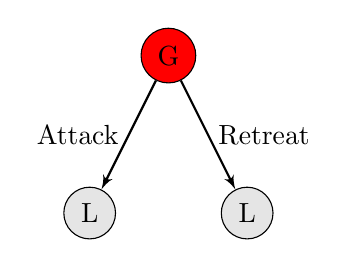
\begin{tikzpicture}
		\node[circle,draw,fill=red, minimum size=0.5] (G) at (0, 0) {G};
		\node[circle,draw,fill=gray!20, minimum size=0.5] (L1) at (-1, -2) {L};
		\node[circle,draw,fill=gray!20, minimum size=0.5] (L2) at (1, -2) {L};
		\draw[-latex', thick] (G) -- (L1) node[midway, left]{Attack};
		\draw[-latex', thick] (G) -- (L2) node[midway, right]{Retreat};
	\end{tikzpicture}
\end{center}

What are lieutenants to do? In the imperfect world of Byzantium the lieutenants can try to figure out if they're about to be mismanaged to literal death by communicating with one another. If they are all on the same page then they can do what they're supposed to do; if they're not, then they will fall back on the default option.

Unfortunately, though, letting the lieutenants communicate is not a complete solution. Because lieutenants can lie, even if the general doesn't.

\begin{center}
	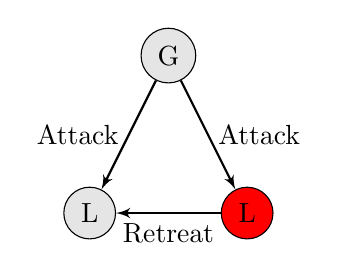
\begin{tikzpicture}
		\node[circle,draw,fill=gray!20, minimum size=0.5] (G) at (0, 0) {G};
		\node[circle,draw,fill=gray!20, minimum size=0.5] (L1) at (-1, -2) {L};
		\node[circle,draw,fill=red, minimum size=0.5] (L2) at (1, -2) {L};
		\draw[-latex', thick] (G) -- (L1) node[midway, left]{Attack};
		\draw[-latex', thick] (G) -- (L2) node[midway, right]{Attack};
		\draw[-latex', thick] (L2) -- (L1) node[midway, below]{Retreat};
	\end{tikzpicture}
\end{center}

In general if there are $d$ disloyal participants, we will need there to be more than $3d$ participants for the loyal lieutenants to agree on what to do. If the general is loyal, then at least $2d$ loyal lieutenants are needed to obey the orders; if the general is disloyal then $2d+1$ loyal lieutenants are needed so they can come up with a course of action~\cite{mte241}.

Let's imagine that there is at most one disloyal participant. If that's the case then all lieutenants should compare notes and decide on the majority course of action. Each lieutenant compiles a little table (or array or vector, whatever) of the data received and then decide on what the majority cause of action is. It might be simpler to just count the total number of votes, but it would make it harder to figure out later who the traitor is (if there is one).

What if we can have two disloyal participants? Each lieutenant sending its messages and using a majority-wins vote isn't necessarily going to work here. It can happen that the general is disloyal and one of the lieutenants is a collaborator. Consider this scenario below from~\cite{mte241} where the general is disloyal and sends mixed instructions. What can the collaborating lieutenant do to make sure that the other lieutenants don't come to an agreement?

\begin{center}
	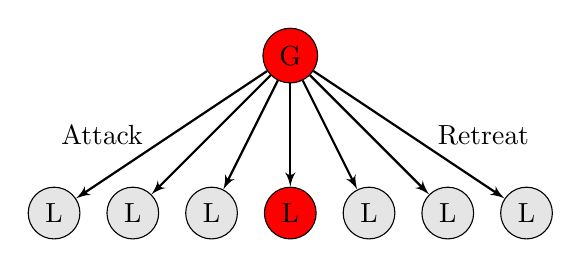
\begin{tikzpicture}
		\node[circle,draw,fill=red, minimum size=0.5] (G) at (0, 0) {G};
		\node[circle,draw,fill=gray!20, minimum size=0.5] (L1) at (-3, -2) {L};
		\node[circle,draw,fill=gray!20, minimum size=0.5] (L2) at (-2, -2) {L};
		\node[circle,draw,fill=gray!20, minimum size=0.5] (L3) at (-1, -2) {L};
		\node[circle,draw,fill=red, minimum size=0.5] (L4) at (0, -2) {L};
		\node[circle,draw,fill=gray!20, minimum size=0.5] (L5) at (1, -2) {L};
		\node[circle,draw,fill=gray!20, minimum size=0.5] (L6) at (2, -2) {L};
		\node[circle,draw,fill=gray!20, minimum size=0.5] (L7) at (3, -2) {L};

		\draw[-latex', thick] (G) -- (L1) node[midway, left]{Attack~~~};
		\draw[-latex', thick] (G) -- (L2);
		\draw[-latex', thick] (G) -- (L3);
		\draw[-latex', thick] (G) -- (L4);
		\draw[-latex', thick] (G) -- (L5);
		\draw[-latex', thick] (G) -- (L6);
		\draw[-latex', thick] (G) -- (L7) node[midway, right]{~~Retreat};
	\end{tikzpicture}
\end{center}

The lieutenants all send one another their instructions. Each of the loyal lieutenants sends its received command and received the honest answer from three other lieutenants. The score is 3 attack and 3 retreat. The disloyal lieutenant sends one message to half the other participants, and a different message to the other half.

\begin{center}
	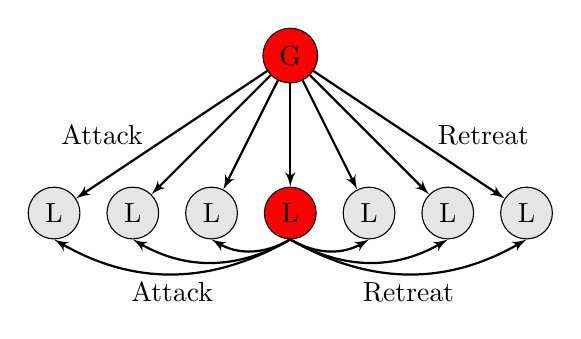
\begin{tikzpicture}
		\node[circle,draw,fill=red, minimum size=0.5] (G) at (0, 0) {G};
		\node[circle,draw,fill=gray!20, minimum size=0.5] (L1) at (-3, -2) {L};
		\node[circle,draw,fill=gray!20, minimum size=0.5] (L2) at (-2, -2) {L};
		\node[circle,draw,fill=gray!20, minimum size=0.5] (L3) at (-1, -2) {L};
		\node[circle,draw,fill=red, minimum size=0.5] (L4) at (0, -2) {L};
		\node[circle,draw,fill=gray!20, minimum size=0.5] (L5) at (1, -2) {L};
		\node[circle,draw,fill=gray!20, minimum size=0.5] (L6) at (2, -2) {L};
		\node[circle,draw,fill=gray!20, minimum size=0.5] (L7) at (3, -2) {L};

		\draw[-latex', thick] (G) -- (L1) node[midway, left]{Attack~~~};
		\draw[-latex', thick] (G) -- (L2);
		\draw[-latex', thick] (G) -- (L3);
		\draw[-latex', thick] (G) -- (L4);
		\draw[-latex', thick] (G) -- (L5);
		\draw[-latex', thick] (G) -- (L6);
		\draw[-latex', thick] (G) -- (L7) node[midway, right]{~~Retreat};
		\draw[-latex', thick] (L4.south) to [bend right] (L7.south);
		\draw[-latex', thick] (L4.south) to [bend right] (L6.south);
		\draw[-latex', thick] (L4.south) to [bend right] (L5.south);
		\draw[-latex', thick] (L4.south) to [bend left] (L3.south);
		\draw[-latex', thick] (L4.south) to [bend left] (L2.south);
		\draw[-latex', thick] (L4.south) to [bend left] (L1.south);

		\node at(-1.5, -3) {Attack};
		\node at(1.5, -3) {Retreat};
	\end{tikzpicture}
\end{center}

Now we're in trouble because half the participants think the majority action is attack and half the participants think the majority action is retreat. Summing up what we heard is not sufficient. Lieutenants should also talk about what they heard from one another. After the general issues instructions, each lieutenant should then communicate with every other to hear what the general said to them. Then by reviewing this information, they can decide what to do.

Consider a simple example where the general is loyal and we have two traitorous lieutenants with a total of seven participants. The general issued an order to attack.

\begin{center}
	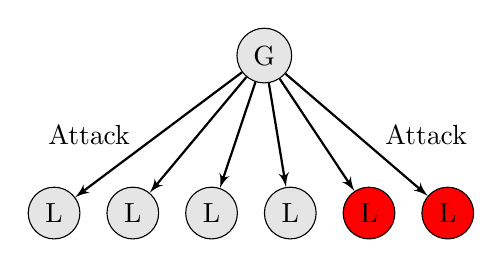
\begin{tikzpicture}
		\node[circle,draw,fill=gray!20, minimum size=0.5] (G) at (-0.33, 0) {G};
		\node[circle,draw,fill=gray!20, minimum size=0.5] (L1) at (-3, -2) {L};
		\node[circle,draw,fill=gray!20, minimum size=0.5] (L2) at (-2, -2) {L};
		\node[circle,draw,fill=gray!20, minimum size=0.5] (L3) at (-1, -2) {L};
		\node[circle,draw,fill=gray!20, minimum size=0.5] (L4) at (0, -2) {L};
		\node[circle,draw,fill=red, minimum size=0.5] (L5) at (1, -2) {L};
		\node[circle,draw,fill=red, minimum size=0.5] (L6) at (2, -2) {L};

		\draw[-latex', thick] (G) -- (L1) node[midway, left]{Attack~~~};
		\draw[-latex', thick] (G) -- (L2);
		\draw[-latex', thick] (G) -- (L3);
		\draw[-latex', thick] (G) -- (L4);
		\draw[-latex', thick] (G) -- (L5);
		\draw[-latex', thick] (G) -- (L6) node[midway, right]{~~Attack};
	\end{tikzpicture}
\end{center}


So each lieutenant constructs the following vector. We're not sure if the general is a traitor, but we'll take notes from every other participant, and see what they report. The general form is as follows, where $v_{x}$ is the forwarded order we received from lieutenant $x$:

\begin{center}
	\begin{tabular}{|l|l|l|l|l|l|l|l|}
		\hline
		General & L1      & L2      & L3      & L4      & L5      & L6      \\
		\hline
		?       & $v_{1}$ & $v_{2}$ & $v_{3}$ & $v_{4}$ & $v_{5}$ & $v_{6}$ \\
		\hline
	\end{tabular}
\end{center}

So if we are lieutenant 1, we complete the table as below. The value for L1 is what we received from the general, but we get the remaining values from the other lieutenants.

\begin{center}
	\begin{tabular}{|l|l|l|l|l|l|l|l|}
		\hline
		General & L1 & L2 & L3 & L4 & L5 & L6 \\
		\hline
		?       & A  & A  & A  & A  & R  & R  \\
		\hline
	\end{tabular}
\end{center}


Then the lieutenants just compare notes on this subject as well! They send to one another their vectors and assemble them into a table. Whatever lieutenant $x$ received in the first round forms row $x$ of the table, and the other rows are added from this second round of communication. In the table each value $v_{i,j}$ is interpreted as ``Lieutenant $i$ says that Lieutenant $j$ reports the general said $v$''. The entries on the diagonal are redundant because of course each lieutenant agrees with itself:

\begin{center}
	\begin{tabular}{|l|l|l|l|l|l|l|l|}
		\hline
		General & L1        & L2        & L3        & L4        & L5        & L6        \\
		\hline
		?       & $v_{1,1}$ & $v_{1,2}$ & $v_{1,3}$ & $v_{1,4}$ & $v_{1,5}$ & $v_{1,6}$ \\\hline
		?       & $v_{2,1}$ & $v_{2,2}$ & $v_{2,3}$ & $v_{2,4}$ & $v_{2,5}$ & $v_{2,6}$ \\\hline
		?       & $v_{3,1}$ & $v_{3,2}$ & $v_{3,3}$ & $v_{3,4}$ & $v_{3,5}$ & $v_{3,6}$ \\\hline
		?       & $v_{4,1}$ & $v_{4,2}$ & $v_{4,3}$ & $v_{4,4}$ & $v_{4,5}$ & $v_{4,6}$ \\\hline
		?       & $v_{5,1}$ & $v_{5,2}$ & $v_{5,3}$ & $v_{5,4}$ & $v_{5,5}$ & $v_{5,6}$ \\\hline
		?       & $v_{6,1}$ & $v_{6,2}$ & $v_{6,3}$ & $v_{6,4}$ & $v_{6,5}$ & $v_{6,6}$ \\\hline
	\end{tabular}
\end{center}

Those ``redundant'' entries (the ones on the diagonal) need to be removed from the table. From the point of view of lieutenant 1, let's imagine the table looks like this (filling in for the sake of the example that L5 and L6 always say retreat).
\begin{center}
	\begin{tabular}{|l|l|l|l|l|l|l|l|}
		\hline
		General & L1 & L2 & L3 & L4 & L5 & L6 \\
		\hline
		?       & ~  & A  & A  & A  & R  & R  \\ \hline
		?       & A  & ~  & A  & A  & R  & R  \\ \hline
		?       & A  & A  & ~  & A  & R  & R  \\ \hline
		?       & A  & A  & A  & ~  & R  & R  \\ \hline
		?       & R  & R  & R  & R  & ~  & R  \\ \hline
		?       & R  & R  & R  & R  & R  & ~  \\ \hline
	\end{tabular}
\end{center}

One the thing we can do, however, is fill in the first column: lieutenant 1 does not care what other people THINK they said; so the whole column can be replaced with what was actually said:

\begin{center}
	\begin{tabular}{|l|l|l|l|l|l|l|l|}
		\hline
		General & L1 & L2 & L3 & L4 & L5 & L6 \\
		\hline
		?       & ~  & A  & A  & A  & R  & R  \\ \hline
		?       & A  & ~  & A  & A  & R  & R  \\ \hline
		?       & A  & A  & ~  & A  & R  & R  \\ \hline
		?       & A  & A  & A  & ~  & R  & R  \\ \hline
		?       & A  & R  & R  & R  & ~  & R  \\ \hline
		?       & A  & R  & R  & R  & R  & ~  \\ \hline
	\end{tabular}
\end{center}

Then we'll try to figure out the majority vote for each $j$ in the table. So sum up each column:

\begin{center}
	\begin{tabular}{|l|l|l|l|l|l|l|l|}
		\hline
		General & L1 & L2 & L3 & L4 & L5 & L6 \\
		\hline
		?       & A  & A  & A  & A  & R  & R  \\
		\hline
	\end{tabular}
\end{center}

And we have four lieutenants who think the general said attack and two who think the general said retreat. The majority wins and the attack proceeds. Onward to victory, brothers and sisters!

If there was one less loyal lieutenant, though, we could have a tie here which would result in picking the default value. If the general ordered something other than the default value (e.g., default is retreat and the order was attack) the general will not be happy about this...

You may have figured out that since disloyal participants can lie at any step of the equation, we can't rely on their data at all. That's true! In the examples in the course we know that two participants are traitors and I've said they are L5 and L6. Therefore we could replace whatever they say with a question mark in the able rather than any particular answer, because they are liars. In real life though, \textit{some} message is received -- attack or retreat -- and it's only later we could identify which participants are the traitors.

Let's go back to the example of having eight participants: one general and seven lieutenants. So if we are lieutenant 1, we complete the table as below. The value for L1 is what we received from the general, but we get the remaining values from the other lieutenants.

\begin{center}
	\begin{tabular}{|l|l|l|l|l|l|l|l|}
		\hline
		General & L1 & L2 & L3 & L4 & L5 & L6 & L7 \\
		\hline
		?       & A  & A  & A  & A  & R  & R  & R  \\
		\hline
	\end{tabular}
\end{center}

However, if we are lieutenant 7 our vector looks like this instead:

\begin{center}
	\begin{tabular}{|l|l|l|l|l|l|l|l|}
		\hline
		General & L1 & L2 & L3 & L4 & L5 & L6 & L7 \\
		\hline
		?       & A  & A  & A  & R  & R  & R  & R  \\
		\hline
	\end{tabular}
\end{center}

From the point of view of lieutenant 1 the table is formed then as follows:

\begin{center}
	\begin{tabular}{|l|l|l|l|l|l|l|l|}
		\hline
		General & L1 & L2 & L3 & L4 & L5 & L6 & L7 \\
		\hline
		?       & ~  & A  & A  & A  & R  & R  & R  \\ \hline
		?       & A  & ~  & A  & A  & R  & R  & R  \\ \hline
		?       & A  & A  & ~  & A  & R  & R  & R  \\ \hline
		?       & ?  & ?  & ?  & ~  & ?  & ?  & ?  \\ \hline
		?       & A  & A  & A  & R  & ~  & R  & R  \\ \hline
		?       & A  & A  & A  & R  & R  & ~  & R  \\ \hline
		?       & A  & A  & A  & R  & R  & R  & ~  \\ \hline
	\end{tabular}
\end{center}

The fourth row is shown as all question marks. Why? Lieutenant 4 is the traitor and could also lie about what the other lieutenants said. Then replace the first column.

\begin{center}
	\begin{tabular}{|l|l|l|l|l|l|l|l|}
		\hline
		General & L1 & L2 & L3 & L4 & L5 & L6 & L7 \\
		\hline
		?       & ~  & A  & A  & A  & R  & R  & R  \\ \hline
		?       & A  & ~  & A  & A  & R  & R  & R  \\ \hline
		?       & A  & A  & ~  & A  & R  & R  & R  \\ \hline
		?       & A  & ?  & ?  & ~  & ?  & ?  & ?  \\ \hline
		?       & A  & A  & A  & R  & ~  & R  & R  \\ \hline
		?       & A  & A  & A  & R  & R  & ~  & R  \\ \hline
		?       & A  & A  & A  & R  & R  & R  & ~  \\ \hline
	\end{tabular}
\end{center}

Sum up each column:

\begin{center}
	\begin{tabular}{|l|l|l|l|l|l|l|l|}
		\hline
		General & L1 & L2 & L3 & L4 & L5 & L6 & L7 \\
		\hline
		?       & A  & A  & A  & ?  & R  & R  & R  \\
		\hline
	\end{tabular}
\end{center}

Each of the lieutenants figures out that we have a draw and we then choose the default choice. Well, that's grim, but it makes sense: the general issued contradictory orders and the collaborating lieutenant did the same. But now instead of half the lieutenants charging in and dying while the others hang back and watch, everyone takes the same action, even if it's not the one that helps the Empire the most.

If there three disloyal participants can exist in the system there's another round of data exchange that needs to take place. Each lieutenant sends the table formed in the second round to all other lieutenants. The more disloyalty there could be in the system, the more rounds the process will go on. As you may have identified, for $n$ participants the communication grows at $n^{2}$ (well, actually worst case $dn^{2}$~\cite{mte241}) and even worse than that, as the number of participants and rounds increases, the amount of data to be sent also increases. For this reason it is somewhat impractical to tolerate a large number of disloyal participants.

That is, however, still a design decision...

Part of the difficulty comes from the fact that lieutenants can lie about what the general said.  In the time of Byzantium, wax seals were used (hot wax is poured and then a stamp or ring was used to make an imprint on it). In modern times messages can be signed using public-key cryptography. Then participants can check whether the received message was genuine. An order that does not appear genuine can be disregarded, reducing the ability of disloyal lieutenants to cause confusion.

The Byzantine Generals Problem has applicability in all kinds of systems, from space flight to cryptocurrency. Whenever we have multiple ``agents'' of some sort that come to their own conclusions about what to do, we can face this issue. As long as we know this, we can design our system with this in mind, because pretending it's not going to happen is not a real solution...








\chapter*{27 --- Concurrency in File Systems}

\addcontentsline{toc}{chapter}{27 --- Concurrency in File Systems}

\section*{Concurrency in File Systems}

To understand the idea of concurrency in file systems, we need to peel back the interface a bit and have at least a high-level understanding of their implementation. File can be of arbitrary size (although in a particular file system there may be a limit), so they have to be allocated on disk according to some strategy.

The contiguous allocation strategy means that a file occupies a set of contiguous blocks on disk. So a file is allocated, starting at block $b$ and is $n$ blocks in size, the file takes up blocks $b, b+1, b+2, ..., b+(n-1)$. But for a sufficiently large file, it might be difficult to find a place to put it. And we also don't know how to predict the size of a file, so how much space do we leave for where to put it?

Linked allocation is a solution to the problems of contiguous allocation: instead of a file being all in consecutive blocks, we maintain a linked list of the blocks, and the blocks themselves may be located anywhere on the disk. The directory listing just has a pointer to the first and last blocks (head and tail of the linked list). Unfortunately, however, accessing block $i$ of a file is no longer as simple as computing an offset from the first block; it requires following $i$ pointers (a pain). If we want to go to the middle of a file, why do we have to load every block on the way there?

There's a compromise approach: indexed allocation. The idea of indexed allocation is to take all the pointers and put them into one location: an index block. So, the first block of the file contains a whole bunch of pointers. To get to block $i$, just go to index $i$ of the index block and we can get the location of block $i$ much more efficiently than we could in linked allocation. All pointers to blocks start as null, and when we add a new block, add its corresponding entry into the index block~\cite{osc}. See the diagram below:

\begin{enumerate}
	\item \textbf{Linked Scheme}: An index block is a disk block, and we can link together several index blocks. The last entry in the index block is either null or a pointer to the next index block.
	\item \textbf{Multilevel Index}: A variant of the linked scheme that has multiple levels. The first level block points to the second level block; the second level block points to the actual file data. This can go to as many levels are necessary based on the maximum file size. If a block is 4~KB, we can have 1024 4-byte pointers, so two levels would allow a maximum file size of up to 4~GB.
	\item \textbf{Combined Scheme}: The all-of-the-above option. This is used in UNIX. Keep the first 15 pointers of the index block in the inode structure; 12 of them point directly to file data. The next three pointers refer to indirect blocks. The 13th is an index block containing the addresses of blocks with data. The 14th points to a double indirect block (addresses of blocks containing addresses of blocks). The 15th points to a triple indirect block\footnote{Yo dawg, we heard you like index blocks...}.
\end{enumerate}

With that out of the way, we can show a visual representation of an inode. This is just another sort of data structure, except it is stored in persistent storage. It will be helpful to keep this in mind. When we lock a file, implicitly we need to know which inode we are locking.

\begin{center}
	\includegraphics[width=0.6\textwidth]{images/unix-inode.png}\\
	The UNIX inode. Triple indirection is left to the reader's imagination~\cite{osc}.
\end{center}

We already discussed the use of \texttt{flock()} to lock a file, and this locks the entire file. There exists another way to lock a file, using \texttt{fcntl}, in which case we can lock only a part of a file, specifically a byte range of that file. This is referred to as \textit{record locking}.

Locking just a part of the file allows for more concurrency: if a process is writing the beginning of the file, another one can be writing the end of the file and these don't overlap so the second write does not need to wait. Let's see how to do that. The function is found in the header \texttt{fcntl.h}. Here's the function signature:

\begin{lstlisting}[language=C]
int fcntl( int file_descriptor, int command, ... /* struct flock * flockptr */ )
\end{lstlisting}

This one looks strange! It turns out that \texttt{fcntl} can do a lot of things, and only sometimes the third argument is needed. So it is a \texttt{...} (list of args) but we would only fill it with one \texttt{struct flock} if we need to based on the value of \texttt{command}. They could have just overloaded this function, but, well, here we are.

The \texttt{struct flock} has the following definition~\cite{apunix}:
\begin{lstlisting}[language=C]
struct flock {
  short  l_type;   /* F_RDLCK, F_WRLCK, or F_UNLCK */
  short  l_whence; /* SEEK_SET, SEEK_CUR, or SEEK_END */
  off_t  l_start;  /* offset in bytes, relative to l_whence */
  off_t  l_len;    /* length, in bytes; 0 means lock to EOF */
  pid_t  l_pid;    /* returned with F_GETLK */
};
\end{lstlisting}

Much like the readers-writers locks, the types of locks are read and write. The compatibility matrix is exactly what you would expect: read locks are compatible with other read locks; write locks are not compatible with any other lock. And finally, to unlock, you still use the set-lock functionality, but with type \texttt{F\_UNLCK}. This sort of locking scheme is vulnerable to deadlock, as it's possible for a process to lock file 1 and need file 2 while another process has a lock on file 2 and needs the lock on file 1.

The value of \texttt{l\_whence} is going to be one of the three constants named in the comment above. This refers to where the offset begins. \texttt{SEEK\_SET} means at the start of the file. So if you specify \texttt{SEEK\_SET} and an offset of \texttt{1000} it means the locked region begins 1000 bytes after the start of the file. \texttt{SEEK\_END} means the relative point is the end of the file. Finally, \texttt{SEEK\_CUR} means based on the current position in the file (if you've positioned within the file using \texttt{seek()} this makes sense).

It is possible for a locked region to extend past the end of the file. This is used when appending to the file, so you don't have to know in advance how much you plan to append to the file. If 0 is given for the length that does include anything appended to the file as well.


For \texttt{command}, our choices are~\cite{apunix}:
\begin{itemize}
	\item \texttt{F\_GETLK} -- Determine if the lock described by \texttt{flockptr} is blocked by some other lock. If a lock exists, the content of \texttt{flockptr} is overwritten with the data of the lock; if no lock exists then the \texttt{l\_type} field is set to \texttt{F\_UNLCK}.
	\item \texttt{F\_SETLK} -- Set the lock as described by \texttt{flockptr}. If the lock cannot be acquired then the return value of the function returns an error and \texttt{errno} are set. This is ``trylock''-behaviour and can be used to avoid the possibility of a deadlock.
	\item \texttt{F\_SETLKW} -- A blocking version of the \texttt{F\_SETLK} command. If the region we want to lock is currently in use then the caller gets blocked.
\end{itemize}

When unlocking a region, just as for locking, you can specify what part of the file you would like to unlock. Partial unlocking is unusual, but why not? The system will combine or split locks as appropriate, based on what is to be locked or unlocked.

Let's do some examples on how to use this structure and system call. The first example is how to lock a file and then how to unlock it:

\begin{lstlisting}[language=C]
int write_lock_file( int file_descriptor ) {

  struct flock fl;
  fl.l_type = F_WRLOCK;
  fl.l_start = 0;
  fl.l_whence = SEEK_SET;
  fl.l_len = 0;
  
  return fcntl( fd, F_SETLK, &fl );
}

int unlock_file( int file_descriptor ) {

  struct flock fl;
  fl.l_type = F_UNLCK;
  fl.l_start = 0;
  fl.l_whence = SEEK_SET;
  fl.l_len = 0;
  
  return fcntl( fd, F_SETLK, &fl );
}
\end{lstlisting}

Obviously if you wished to have a different type of lock or to only lock a specific range, then you would need different values in the structure. Now for checking if a given part of a file is locked:

\begin{lstlisting}[language=C]
int fd = open ( "example.txt", O_RDONLY );
struct flock lock;

lock.l_type = F_RDLOCK;
lock.l_start = 1024;
lock.l_whence = SEEK_SET;
lock.l_len = 256;

fcntl( fd, F_GETLK, &lock );
if ( lock.l_type == F_UNLCK ) {
	/* Lock is unlocked; we may proceed */
} else if ( lock.l_type = F_WRLOCK ) {
  /* File is write locked by a different process */
  printf( "File locked by process ID %d.\n", lock.l_pid );
  return -1;
}
\end{lstlisting}

Checking on things with \texttt{F\_GETLK} is really for information purposes only: you should not make decisions about whether to proceed based on this, because of course the sequence of ``read of the value and then whatever operation you'd like to do next'' is not atomic. Instead, use the command \texttt{F\_SETLK} and actually try to set the lock. If \texttt{-1} is returned then locking was not successful. Or, if the plan is to wait, use \texttt{F\_SETLKW} as one would expect.

It's important to remember that \texttt{fcntl} changes some values of the \texttt{struct lock} so if you wanted to re-use it you need to make sure to reset it as appropriate. You can use the same \texttt{struct lock} later to unlock the thing that you locked, just do so carefully.

I'll also take a minute to mention \texttt{lockf}: it is a simplified way of locking a file. While \texttt{fcntl} is more flexible, sometimes all we need is the simple version. According to the documentation:

\begin{lstlisting}[language=C]
int lockf( int file_descriptor, int command, off_t length );
\end{lstlisting}

The command options can be:
\begin{itemize}
	\item \texttt{F\_LOCK} -- Acquire an exclusive lock on the (section of the) file.
	\item \texttt{F\_TLOCK} -- Try to acquire an exclusive lock (try-lock behaviour).
	\item \texttt{F\_ULOCK} -- Unlock the indicated section of the file.
	\item \texttt{F\_TEST} -- Check if (a section of) the file is locked; 0 if it is unlocked and -1 if the file is locked.
\end{itemize}


The length is an offset, and is based off the current position in the file. If zero is provided then it locks the whole file.

Two further notes: The file is automatically unlocked when the file descriptor is closed. And, on some systems \texttt{lockf} just calls \texttt{fcntl} but on some others they use different mechanisms. So don't mix and match. If you lock a file with one function, unlock it with the matching one.

It is noteworthy that both kinds of lock are ``advisory'' only. That is, like the use of a semaphore or mutex, it only is really effective if everyone involved in accessing the shared resource follows the proper protocol and checks if access is permitted or not. Mandatory locks do exist, but are hard to use and are not recommended. Did you really want to know about mandatory locking? Well, check out this kernel.org documentation as to why you shouldn't, but also how it works if you must: \url{https://www.kernel.org/doc/Documentation/filesystems/mandatory-locking.txt}.

\subsection*{Using A File as a Lock}

We can use the very existence of a file as a way of controlling concurrency. For example, \texttt{git} places a file \texttt{index.lock} in a particular directory to indicate that an operation is in progress so two different \texttt{git} clients do not operate on the same repository at the same time. So that is one strategy: check if the file is present; if it is, the resource is ``locked'', if no such file is present then it is ``unlocked''.

If we want to check, we just try to \texttt{open()} the file, but unless we are careful this can lead to a problem if two processes want to create the file: if they both call \texttt{open}, they both might succeed. To get around this, we need to use the \texttt{flags} parameter of the call to open the file. See below.

\begin{lstlisting}[language=C]
int open(const char *filename, int flags);  /* Returns a file descriptor if successful, -1 on error */
int rename(const char *old_filename, const char *new_filename); /* Returns 0 on success , operates atomically */
int remove(const char *filename) ; /* Deletes a file or directory, returns 0 on success, operates atomically */ 
\end{lstlisting}

When opening a file the following flags may be used for the \texttt{flags} parameter (and can be combined with bitwise OR, the \texttt{|} operator):

\begin{tabular}{l|l}
	\textbf{Value}     & \textbf{Meaning}                                                                                 \\ \hline
	\texttt{O\_RDONLY} & Open the file read-only                                                                          \\ \hline
	\texttt{O\_WRONLY} & Open the file write-only                                                                         \\ \hline
	\texttt{O\_RDWR}   & Open the file for both reading and writing                                                       \\ \hline
	\texttt{O\_APPEND} & Append information to the end of the file                                                        \\ \hline
	\texttt{O\_TRUNC}  & Initially clear all data from the file                                                           \\ \hline
	\texttt{O\_CREAT}  & Create the file                                                                                  \\ \hline
	\texttt{O\_EXCL}   & If used with \texttt{O\_CREAT}, the caller MUST create the file; if the file exists it will fail \\
\end{tabular}

We can combine the use of \texttt{open} with \texttt{rename} to get lock-like behaviour between different programs that share nothing except a common file system. The \texttt{open} call should be used to create the lock file, and fail if the file already exists. If we want we can use \texttt{remove} to delete the lock file if we want to let the next process try, but there's an alternative option: \texttt{rename}.

Because the \texttt{rename} function is also atomic, we can use it too, and just rename the existing lock file rather than creating it and deleting it every time. Then programs that want their turn should use \texttt{rename}; if a process or thread does succeed in renaming the file it is that process or thread's turn; otherwise, they have to wait. To unlock, just change the name back. Consider this simple example that uses threads (rather than processes):

\begin{lstlisting}[language=C]
#include <stdio.h>
#include <stdlib.h>
#include <fcntl.h>
#include <unistd.h>
#include <sys/stat.h>
#include <sys/types.h>
#include <pthread.h>

#define NUM_THREADS 10

int lock_fd;
int shared = 0;

void* run( void* arg ) {
  int* id = (int*) arg;
  while( rename( "file.lock", "file.locked" ) == -1 ) {
    printf("Thread %d waiting.\n", *id); 
  }

  printf("Thread %d in critical section.\n", *id);
  printf("Shared incremented from %d", shared);
  shared++;
  printf(" to %d.\n", shared);
  rename("file.locked", "file.lock"); /* Unlock */

  free( arg );
  pthread_exit(NULL);
}

void* writer( void* arg ) {
  /* Write data implementation not shown */
  pthread_exit(NULL);
}


int main( int argc, char** argv ) {
  lock_fd = open( "file.lock", O_CREAT | O_EXCL );  
  if (lock_fd == -1 ) {
   printf( "File creation failed.\n");
   return -1;
  }

  pthread_t threads[NUM_THREADS];
  for (int i = 0; i < NUM_THREADS; i++) {
    int * id = malloc( sizeof( int ) );
    *id = i;
    pthread_create( &threads[i], NULL, run, id );
  }
  for (int i = 0; i < NUM_THREADS; i++) {
    pthread_join( threads[i], NULL );
  }
  close( lock_fd );
  remove( "file.lock" );

  return 0;
}
\end{lstlisting}








\chapter*{28 --- More Concurrency in File Systems}

\addcontentsline{toc}{chapter}{28 --- More Concurrency in File Systems}

\section*{Concurrency in File Systems, Continued}


\subsection*{Copy-Modify-Merge}
Thus far when we talk about modification of shared data we follow a model that could be described as ``Lock-Modify-Unlock''. But you've also used \texttt{git} or some other version control system (\texttt{svn}) that uses a different model: Copy-Modify-Merge. Let's take a minute to talk about that.

Using \texttt{git} or something else, you and your lab partner check out a repository. You make changes and then try to merge those changes. When changes are being applied, we want to make sure that all changes in a particular grouping (in version control, a commit) either succeed as a group or fail as a group and nothing is left half-done.

A \textit{transaction} is a grouping of operations that belong together and should be treated as an indivisible unit. You will recall from a great deal of discussion on the subject of concurrency that bad things can happen when an intermediate state of a multiple-step operation becomes inadvertently visible. Most of the examples looked at things like \texttt{x++;} being a read, addition, and a write and how concurrent accesses to \texttt{x} could result in the wrong value being read or written. The solution is usually mutual exclusion: forcing other accesses to \texttt{x} to wait while some operation was in progress. And this of course also scales up so you could change \texttt{x, y, z, a, b, c} all in one go. But in the copy-modify-merge scenario, people can make their changes separately and then we try to put them all together.

A transaction has some sort of begin transaction statement at the beginning, then the operations to take place in the transaction, and finally an end transaction statement. Execution looks something like writing down the transaction into a log, doing the operations in the transaction, and when the last one is complete, if all went well, marking the transaction as successful.

In the case of version control, if there are merge conflicts then we are notified that the merge cannot take place until conflicts are resolved. But in file systems, the last write wins.

\subsection*{You Have 15 Unread Notifications...}

Another way that we can use the file system (in Linux only!) for synchronization or concurrency control is through the use of \texttt{inotify}. Using this API, you can register your program as being interested in the events in the file system. We'll come back to a definition of what an event is soon. But in short, you say you want to watch a file or directory, and when an event occurs, then your program is informed. Note that this is not a portable thing: it is Linux only.

The key steps are~\cite{lpi}:
\begin{enumerate}
	\item Use an initialization function to create the management structure (and get a file descriptor back to refer to it).
	\item Then you tell the kernel what files you are interested in by adding them to the structure (you can also remove them).
	\item To collect an event, use \texttt{read} on the file descriptor. Each call returns one or more event structures.
	\item If you're done, close the file descriptor representing the management structure, which conveniently cleans everything up for you.
\end{enumerate}

It is noteworthy that the mechanism is not recursive: so if you add a directory, that covers the files in that directory, but not subdirectories.

The API calls:
\begin{lstlisting}[language=C]
int inotify_init( ); /* Returns file descriptor referring to the struct */
int inotify_add_watch( int fd, const char* pathname, uint32_t mask );
int inotify_rm_watch( int fd, uint32_t wd );
\end{lstlisting}

Initialization doesn't require any arguments, so that's quite convenient.

Adding an item to the watch takes as an argument the inotify structure to add it to, the name of the file to add, and a mask. You must have at least read permission on the file to be able to watch it. The mask is how we specify details about the events that we are interested in (we'll come back to that). If the file is already being watched, then calling add with a different mask will replace the mask with the new one.

We have to save the return value of the add function if we want to use the remove function, because it takes that return value as an argument. The remove function says remove the given watch item from the list.

When we're completely done, just call close on the file descriptor representing the inotify.

There are about 23 different events that you can watch for using the bit mask. Some of them are a bit obscure, but here are some that are highlighted in the spec:

\begin{center}
	\begin{tabular}{l|l}
		\textbf{Bit Value}          & \textbf{Description}                             \\ \hline
		\texttt{IN\_ACCESS}         & File accessed (read/execute)                     \\
		\texttt{IN\_ATTRIB}         & Metadata changed, such as permissions            \\
		\texttt{IN\_CLOSE\_WRITE}   & File opened for writing was closed               \\
		\texttt{IN\_CLOSE\_NOWRITE} & File not opened for writing was closed           \\
		\texttt{IN\_CREATE}         & File or directory created in watched directory   \\
		\texttt{IN\_DELETE}         & File or directory deleted from watched directory \\
		\texttt{IN\_DELETE\_SELF}   & Watched file or directory deleted                \\
		\texttt{IN\_MODIFY}         & File modified (write, for example)               \\
		\texttt{IN\_OPEN}           & File opened                                      \\
		\texttt{IN\_ALL\_EVENTS}    & Watch for all of the above (and a few more)
	\end{tabular}
\end{center}

Great, so imagine we have set up some files that we would like to watch. When you're ready for such an event, use \texttt{read} on the file descriptor for the inotify. If an event occurred, you get back a structure \texttt{inotify\_event} that looks like this (as described in the official docs):

\begin{lstlisting}[language=C]
struct inotify_event {
  int      wd;       /* Watch descriptor */
  uint32_t mask;     /* Mask describing event */
  uint32_t cookie;   /* Unique cookie associating related events (for rename(2)) */  
  uint32_t len;      /* Size of name field */
  char     name[];   /* Optional null-terminated name */
};
\end{lstlisting}

The first returned value is which file descriptor it was the event happened on, as we'd expect. The second says what kind of event occurred. The third parameter is a delicious, delicious cookie: it allows you to identify a rename operation (if a file is renamed in the directory, this shows up as two events and the cookie is used to link the two). The length field tells you how long the name array is, and then there is of course the name array. That means memory size of an inotify event is thus the structure size plus the length of the array, i.e.: \texttt{sizeof( struct inotify\_event) + len}~\cite{lpi}.

This is something somewhat rare -- usually when we do a read we need to know how many bytes we'd like to read. If we're reading a struct, we know the size of the struct, but now it depends on the length of the data you get back. Your standard clairvoyance problem. One approach is to just make the buffer really big: much bigger than it needs to be. The length of the largest filename plus one (for the null terminator) would work. If your buffer isn't big enough the read call will fail.

Alternatively, \texttt{ioctl} can tell you what you want to know: \texttt{ioctl( fd, FIONREAD, \&numbytes )} updates \texttt{numbytes} with the number of bytes currently available to read from the inotify instance~\cite{lpi}.  If multiple events occurred you can get multiple structures back (if your buffer is big enough).

A relatively simple example then: we'd like to observe when a lock file is deleted, so that we can try to take some action that occurs afterwards. We can demonstrate this program working when we start it and the lock file already exists.

\begin{lstlisting}[language=C]
#include <stdlib.h>
#include <stdio.h>
#include <sys/inotify.h>
#include <stdbool.h>
#include <unistd.h>
#include <fcntl.h>
#include <string.h>

const char filename[] = "file.lock";

int main( int argc, char** argv ) {
    int lockFD;
    bool our_turn = false;
    
    while( !our_turn ) {
        lockFD = open( filename, O_CREAT | O_EXCL | O_TRUNC );
        if ( lockFD == -1 ) {
            printf( "The lock file exists and process %ld will wait its turn...\n", getpid() ); 
            int notifyFD = inotify_init( );
            uint32_t watched = inotify_add_watch( notifyFD, filename, IN_DELETE_SELF );
            
            /* Read the file descriptor for the notify -- we get blocked here
               until there's an event that we want */
            int buffer_size = sizeof( struct inotify_event ) + strlen( filename ) + 1;
            char* event_buffer = malloc( buffer_size );
            printf("Setup complete, waiting for event...\n");
            read( notifyFD, event_buffer, buffer_size );

            struct inotify_event* event = (struct inotify_event*) event_buffer;
            /* Here we can look and see what arrived and decide what to do.
               In this example, we're only watching one file and one type
               of event, so we don't need to make any decisions now */

            printf("Event occurred!\n");

            free( event_buffer );
            inotify_rm_watch( lockFD, watched );
            close( notifyFD );
        } else {
            char* pid = malloc( 32 );
            memset( pid, 0, 32 );
            int bytes_of_pid = sprintf( pid, "%ld", getpid() );

            write( lockFD, pid, bytes_of_pid ); 
            free ( pid );
            close( lockFD );
            our_turn = true; 
        }
    } 

    printf("Process %ld is in the area protected by file lock.\n", getpid());
    remove( filename );
    return 0;
}
\end{lstlisting}

\section*{Consistency: Journalling}

Unfortunately, an error, crash, or power failure may result in a loss of data or inconsistent data in the file system. The directory structures, pointers, inodes, et cetera are all data structures and if they become corrupted it may lead to serious problems.

We could check for inconsistent data periodically (e.g., on system boot up) and many operating systems do so. This is, of course, an operation that will consume a very large amount of time while the whole disk is scanned. The UNIX tool for this is \texttt{fsck} (... not exactly something you want to say out loud) and the Windows tool is \texttt{chkdsk} (check disk). These tools will look for inconsistent states (e.g., a file that claims to be 12 blocks but the linked list contains only 5) and will attempt to repair the data structures. Its level of success depends on the nature of the problem and the implementation of the file system.

Obviously we would like to prevent the problem, if we can. The solution is to use transactions, just as we do in version control. Either a change takes place in its entirety or it is as if it never happened.


\subsection*{ZFS (Sun/Oracle File System)}
Let's consider ZFS (as I understand it, pronounced ``Zee Eff Ess''), which is intended for scalability and has some interesting features. The primary source for this section is the official documentation~\cite{zfs}. Because what better place than from the source?

ZFS uses the idea of transactions, making sure that the state is always consistent on disk. Much like the copy-modify-merge model, data is copied, then changed, then rewritten. Blocks are never overwritten with new data. Instead, a transaction writes all data and metadata to new blocks. Only when the transaction is complete, any references to the old blocks are replaced with the location of the new blocks. Then the old pointers and blocks can be cleaned up (reused or disposed of).

This does have an interesting weakness: if the disk becomes completely and totally full it is not possible to delete anything and make space, because there's no place to allocate new blocks. That's a problem. And not just a hypothetical: it happened to a friend of mine when he tried to put too much data in his NAS (network attached storage). He was mad. But he was going to buy a new one anyway, I guess...

\subsection*{APFS (Apple File System)}

Like some version control systems, APFS brings the ability to take snapshots of the file system: freeze the state of the file system and from there any additional changes are ``diffs'' against that base state, meaning only new things take up space. This is potentially quite helpful for taking backups (you do take backups, right?)~\cite{apfs}.

Speedier backups can result: the performance of your system can be degraded while backups are being taken because you need to compute the difference between the last backup copy and the current. This is faster! But it is also a way to avoid corruption: you can replay changes as needed to get the file back to \textit{a} consistent state (of some sort).

The APFS does potentially harm the most common ``backup'' system of non-technical users: take a copy of the file and put it in a different folder. If you copy a file to the same volume (and make no changes) then APFS will not copy the data and instead just have two references to the same underlying location. It sounds like they're doing you a favour if you think of this as just reducing wasted space, but is actually a negative from the perspective of redundancy: if that part of the disk is damaged then all copies are lost~\cite{apfs}.

Somewhat like ZFS, the APFS approach to avoiding inconsistent data amidst a crash is something like copy-on-write, though in typical Apple fashion they were pretty vague about what this means in a practical sense; the APFS lead developer Dominic Giampaolo just says it's a ``novel copy-on-write metadata scheme'' but also somehow not exactly the same as ZFS's single-atomic-update approach~\cite{apfs}.

\subsection*{NTFS (Windows File System)}
Though UNIX and similar systems have often been a focus of the examples, in this case, we will instead examine NTFS, the default file system for Windows since Windows NT and used in 2000, XP, Vista, 7, 8, 10... NTFS supports large disks and large files, and uses journalling.

A volume is laid out as follows:

\begin{center}
	\includegraphics[width=0.6\textwidth]{images/ntfs-volume.png}\\
	Standard layout of an NTFS volume~\cite{osi}.
\end{center}

The Master File Table (MFT) contains information about all the files and folders. Following the that, a block is allocated to system files that contain some important system information~\cite{osi}:

\begin{enumerate}
	\item \textbf{MFT2}: Mirror of the first few rows of the MFT (in case the original is damaged).
	\item \textbf{Log File}: The journalling transaction log.
	\item \textbf{Cluster Bitmap}: Bitmap showing which of the clusters are in use.
	\item \textbf{Attribute Definition Table}: Attribute types supported on this volume.
\end{enumerate}

NTFS uses journalling to ensure that the file system will be in a consistent state at all times, even after a crash or restart. There is a service responsible for maintaining a log file that will be used to recover in the event that things go wrong.  Note that the goal of recovery is to make sure the system-maintained metadata is in a consistent state; user data can still get lost. This was a decision on the part of Microsoft to make the recovery operations significantly simpler and faster.

All metadata changes are written sequentially to a log file; once the changes are written to the log, control may return to the program that requested the operation. Meanwhile, the log entries are actually carried out. As changes are made, a pointer is updated to indicate which of the log entries have really happened and which have not. When an entire transaction is completed, it is removed from the log file. If the system crashes, the log file will contain zero or more transactions. If there are zero there is no problem: nothing was in progress at the time of the crash. If there are some, then the transactions were not completed and the operations should still be carried out. If a transaction was aborted (not committed), we walk backwards through the log entries to undo any completed operations and go back to the state before the start of the transaction~\cite{osc}.

Even though a particular write may not have taken place because of a crash, resulting in some data loss, at least the system will always remain in a consistent state. As a side benefit, we can sometimes re-order the writes to get better performance (e.g., schedule them in such a way that we get better disk utilization).


The actual implementation of journalling works as follows~\cite{russ}:

\begin{enumerate}
	\item Record the change(s) in the log file in the cache.
	\item Modify the volume in the cache.
	\item The cache manager flushes the log file to disk.
	\item Only after the log file is flushed to disk, the cache manager flushes the volume changes.
\end{enumerate}

What's really interesting about this is that the changes are carried out in the background, that is to say, asynchronously. A program can say that it wants to write some data, and not have to wait for the data to be written before going on to the next thing. How interesting! Can we get that behaviour in our (regular) program? Yes we can...








\chapter*{29 --- Asynchronous I/O with select, poll}

\addcontentsline{toc}{chapter}{29 --- Asynchronous I/O with select, poll}

\section*{Asynchronous (non-blocking) I/O}
Consider some of the usual file read code:

\begin{lstlisting}[language=C]
int fd = open( "example.txt", O_RDONLY );
int bytes_read = read( fd, buffer, num_bytes );
close( fd );
\end{lstlisting}

As we discussed much earlier, the \texttt{read} call is blocking, as expected. So, your program waits for the I/O operation to be complete before continuing on to the next statements (whatever they are). This is sometimes, but not always, sensible. If you need the data in the next statement, you can't go on until the data is present.

If you are waiting for the bus, do you stare off blankly into space while waiting for it to arrive? Probably not. More likely you pull out your phone and start to use it for something. Whether that is productive or not (e.g., answering a project e-mail or liking posts on Facebook) is up to you, but you are doing something and making use of the time.

Our main solution until now is threads: if one thread gets blocked on the I/O the other ones can continue and is fine. But maybe you don't want to use threads, or maybe you can't due to: race conditions, thread stack size overhead, or limitations on the maximum number of threads. The last one might seem ridiculous, but in some embedded system you may not have the option to make new threads (or at least not as many as you want).

Sometimes, also, your programming language (e.g., Javascript) doesn't allow you to make multiple threads and you really have no choice but to use asynchronous I/O. It's a useful tool to have in the toolbox so let's get into it.

The simplest example:

\begin{lstlisting}[language=C]
int fd = open( "example.txt", O_RDONLY | O_NONBLOCK );
int bytes_read = read( fd, buffer, num_bytes ); /* Returns instantly! */
close( fd );
\end{lstlisting}

If we opened the file in non-blocking, the \texttt{read} call returns instantly. Whether or not results are ready. Unfortunately, this doesn't work here. The \texttt{O\_NONBLOCK} option is not helpful, because this call says we should not wait for data when there is no data available. But a file \textit{always} has data available. It might take a long time to load it up from disk, but the data is there. Do we know any scenarios where we don't have data always available?

Sure! Sockets. If we haven't received something, we would get blocked waiting for some data to arrive. But we can change that behaviour on a socket if we wish, by setting the socket to be nonblocking~\cite{getaddrinfo}:

\begin{lstlisting}[language=C]
sockfd = socket( PF_INET, SOCK_STREAM, 0 );
fcntl( sockfd, F_SETFL, O_NONBLOCK );
\end{lstlisting}

This means that calls to \texttt{accept()}, \texttt{recv()}, or \texttt{recvfrom()} would not block. If you call those and there's no data to receive, you get back a return value of \texttt{-1} and \texttt{errno} is going to be either \texttt{EAGAIN} or \texttt{EWOULDBLOCK}. Sadly, the specification does not say which it would be, so the fully correct approach is to check for both. Not great, but it's how we are sure.

Suppose that you are writing a server application that's going to listen on several sockets. This is a common enough scenario. You could have different threads listening on their individual sockets but -- see the reasoning above as to why we might not have that option. And we no longer have to!

But if we are a server and there aren't any incoming requests, what exactly are we supposed to do with our time? If we just poll each socket using, for example, \texttt{accept()}, this amounts to tight polling and is CPU intensive and wastes the CPU's time. But we don't want to get blocked on a particular socket either, because what if it's not the one where the next packet arrives? What we need is a third option.

\subsection*{Third option: \texttt{select()}} Our wish is granted. The third option is called \texttt{select()} -- it allows us to monitor a group of sockets, telling us about the state of each of them. A socket could be ready for a read, ready for a write (of small size -- you can't write a huge chunk to a socket without getting blocked at some point), or whether an exception has occurred. So actually, select works on three sets of sockets:

\begin{lstlisting}[language=C]
 int select( int nfds, fd_set *readfds, fd_set *writefds, fd_set *exceptfds, struct timeval *timeout );
\end{lstlisting}

If we call this function, we'll get blocked until something happens on one of the sockets so that it becomes ``ready'' -- data is available to read, space is available to write, etc. or until we reach a timeout. While blocked, we could also get interrupted by something (e.g., a signal).

The first parameter, \texttt{nfds}, is supposed to be the value of the highest number file descriptor in any of the three sets plus 1. So. It has come to this. One of the problems with \texttt{select()} is that it is pretty... arcane. According to the documentation, the reason why it is this, is because \texttt{select()} will scan through all the file descriptors from 0 up to \texttt{nfds-1} to figure out if we care about them.

What's this about? Well, the \texttt{fd\_set} structure can have up to 1024 file descriptors, and is actually implemented as a bitfield; by specifying the highest file descriptor that we are interested in, the kernel can stop looking once we reached the last one (and the \texttt{fd\_set} structure doesn't have to be a linked list or array or anything large!)~\cite{apunix}.

Well, we were going to have to figure out what the \texttt{fd\_set} means anyway. It represents a set of file descriptors, just as the name says.  There are then four functions for manipulating a set:

\begin{lstlisting}
void FD_ZERO( fd_set *set ); /* Clear the set */
void FD_SET( int fd, fd_set *set ); /* Add fd to the set */
void FD_CLR( int fd, fd_set *set ); /* Remove fd from the set */
int  FD_ISSET( int fd, fd_set *set); /* Tests if fd is a part of the set */ 
\end{lstlisting}

When we create a new set, we should first initialize it with a \texttt{FD\_ZERO} call. That could also be used to reset it, if desired, at some later point. Then we can add file descriptors that we want to have. To add one, use \texttt{FD\_SET} with the file descriptor to add; to remove one that has been added, use \texttt{FD\_CLR} with the file descriptor to remove.

But that last one, \texttt{FD\_ISSET}, is a little different. It's not as if we would forget whether we put a file descriptor in the set. It's really for us to see what happens after \texttt{select()} is called -- we can find out whether a given file descriptor is in a particular set or not.

The \texttt{readfds} are obviously sockets we are interested in reading from and \texttt{writefds} are accordingly those we are interested in writing from. But what about the \texttt{exceptfds} -- this isn't Java, it's not like we're going to get a \texttt{SocketDoesNotFeelLikeDoingWorkRightNowException}. No, this is for sockets that are in an exceptional state, which usually means there is Out-Of-Band (OOB) data on a TCP socket. We didn't cover this earlier in network communication and we will also not be going into this subject now. But you can find out if a socket is in that state if you have a reason.

We don't have to use all three of \texttt{readfds}, \texttt{writefds}, and \texttt{exceptfds} in a call to \texttt{select()} if we do not need them all. If we have only read sockets, we put them all in the \texttt{readfds} set and can just give \texttt{NULL} or empty \texttt{fd\_set}s in for the other parameters~\cite{getaddrinfo}.

Finally, there is a timeout parameter: we can specify a maximum amount of time we  are willing to wait. If nothing happens before the timeout amount of time occurs, then \texttt{select()} returns. The format of this is a fairly simple structure \texttt{struct timeval}:

\begin{lstlisting}[language=C]
struct timeval {
  long tv_sec; /* seconds */
  long tv_usec; /* microseconds */
};
\end{lstlisting}

If both fields of the \texttt{struct timeval} are zero, then \texttt{select()} returns immediately; if the pointer to it is \texttt{NULL} then there is no timeout and we will wait as long as it takes for something -- anything -- to happen.

When \texttt{select()} returns, however that happened, some if not all of the parameters other than \texttt{nfds} got updated (argh). The file descriptors passed in are modified in-place to see if they changed status.  And the \texttt{struct timeval} parameter may (but also may not) be updated to reflect how much time was left before the timeout. Because different systems may or may not change this value, it is not safe to re-use and should be overwritten if you plan to use that structure again.

After select has returned, then we check the file descriptors in our sets. All of them. Yes, really. The function returns when there is something to do -- but we aren't told what socket is ready. So we would need to check each socket to see if, for example, it's ready for reading (if that's the plan). To do that we check \texttt{FD\_ISSET} with the socket and the set to see if it's in the desired state.

Because the sets of file descriptors may have been modified, you probably need to rebuild them after each call, if you plan to use them again. If you were waiting, for example, three sockets, not all of them necessarily became ready at the same time. So if you want to go on waiting for those three, you will need to put them in a set again.

Let's imagine a brief example where we have a server that is going to listen on some different sockets for different services, imaginatively called service1, service2, and service3.

\begin{lstlisting}[language=C]
void listen_for_connections( int service1_sock, int service2_sock, int service3_sock ) {
  int nfds = 1 + (service1_sock > service2_sock
    ? service1_sock > service3_sock ? service1_sock : service3_sock
    : service2_sock > service3_sock ? service2_sock : service3_sock);
    
  fd_set s;
  struct timeval tv;
  printf( "Going to start listening for socket events.\n" );
  
  while( !quit ) {
  
    FD_ZERO( &s );
    FD_SET( service1_sock, &s );
    FD_SET( service2_sock, &s );
    FD_SET( service3_sock, &s );
    
    tv.tv_sec = 30;
    tv.tv_usec = 0;
  
    int res = select( nfds, &s, NULL, NULL, &tv );
    if ( res == -1 ) { /* An error occurred */
      printf( "An error occurred in select(): %s.\n", strerror( errno ) );
      quit = 1;
    } else if ( res == 0 ) { /* 0 sockets had events occur */
      printf( "Still waiting; nothing occurred recently.\n" );
    } else { /* Things happened */
      if ( FD_ISSET( service1_sock, &s ) {
        service1_activate( ); 
      }
      if ( FD_ISSET( service2_sock, &s ) {
        service2_activate( ); 
      }
      if ( FD_ISSET( service3_sock, &s ) {
        service3_activate( ); 
      }
  }
}
\end{lstlisting}

You'll notice that we check each of the sockets individually -- more than one of them could become ready at once. Now, the \texttt{activate()} calls there could take some nontrivial time, and if sockets receive data in the meantime then on the next iteration of the loop then \texttt{select()} will return immediately because data is waiting.

This represents a fairly simple scenario, though, where we are just waiting for \texttt{accept()} on the three services where we send back as simple response and that's the end of it. But if the connections we were looking at are supposed to stay open for some period of time, such as when there is occasional communication, then we would also have to add and remove sockets from the sets as connections were opened and closed. Managing the set of sockets in such a scenario is non-trivial, because each call to \texttt{select} can (and usually does) change the sets.

\paragraph{Chat Server.} The more complicated example in~\cite{getaddrinfo} is about a chat program (if you ever used IRC you have a pretty good idea of how this would work). When people want to join the chat room they send a message to a server. The server accepts and opens the connection and adds the client to the chat room. But people don't always talk. So if nothing is happening right now there's nothing to send. So the server can use \texttt{select()} to keep an eye open for when someone has said something. Either way, we would wait for something to happen, either on one of the sockets from a current client, or the socket for accepting incoming connections.

If it's the socket for accepting incoming connections that activated then accept the incoming connection, and add the new socket to the list that we are going to listen to. A chat server might choose to send a notification to other clients to let them know that a new person has joined the chat. That would be a write to the sockets that represent connected clients.

If another socket activated, most likely someone had something to say. So we can read from the socket that is ready to read and pass on the message that we received to all the other clients. Except, sometimes there isn't one! A socket will show up as being ready for reading if it has closed. But the call to read will return 0 (or a negative number) if the socket has closed (i.e., the client has disconnected). If the connection has been closed, then we should remove that socket from the list that we are interested in. And also we sometimes send a message telling other clients that a person has left the chat.

And when a message is received from a client, then of course the thing for the server to do is to send it on to the other clients, by writing to their sockets so the message is transmitted to them. The clients are waiting to receive messages and will then show them to the user when someone says something. And then look at that: you're talking to other people on the internet! Just remember not to give out your personal information to strangers.

Obviously there are some other considerations that come with managing a chat server. There might be periodic connection-keep-alive kind of messages so that clients remain connected even if nobody is talking right now. And you might want the ability to kick out people who are spammers and perhaps even ban them, amongst other things. But the goal of this explanation wasn't really to learn how to write a chat server in great detail -- just to give an example of how you could use \texttt{select} to write something useful.

\paragraph{Slightly different, mostly the same: \texttt{pselect}.}
There is also \texttt{pselect()} which has the signature:
\begin{lstlisting}[language=C]
int pselect( int nfds, fd_set *readfds, fd_set *writefds, fd_set *exceptfds, 
            const struct timespec *timeout, const sigset_t *sigmask );
\end{lstlisting}

The signature is different in two ways. The first is that instead of \texttt{struct timeval} it is a \texttt{struct timespec}, which is slightly different in its meaning, and also will never be modified by the call to \texttt{pselect}:

\begin{lstlisting}[language=C]
struct timespec {
  long tv_sec; /* seconds */
  long tv_nsec; /* nanoseconds */
};
\end{lstlisting}

Yes, the only real difference is that it is seconds and nanoseconds, rather than seconds and milliseconds. The other parameter is about setting up a signal mask. We discussed the signal mask much earlier on when we talked about signals for interprocess communication. This is the same, but it allows us to change the signal mask atomically in the same step as the call to select, so we can choose what signals are allowed to wake us up while we are waiting for something to happen. Given appropriate allocation and initialization of the values, the call:


\begin{lstlisting}[language=C]
ready = pselect( nfds, &readfds, &writefds, &exceptfds, timeout, &sigmask );
\end{lstlisting}

is equivalent to an atomic operation that does all of:

\begin{lstlisting}[language=C]
sigset_t origmask;
pthread_sigmask( SIG_SETMASK, &sigmask, &origmask );
ready = select( nfds, &readfds, &writefds, &exceptfds, timeout );
pthread_sigmask( SIG_SETMASK, &origmask, NULL );
\end{lstlisting}

If we had tried to do the multi-step sequence then there is always the possibility that something (e.g., a signal!) could happen in between changing the signal mask and the call to \texttt{select}. The syntax here for changing the signal mask is slightly different than what we have seen before, but this is the POSIX specification implementation of the \texttt{sigprocmask()} call. So, it works the same as we have seen earlier.

\paragraph{I only wanted a nap...} It is possible to ``misuse'' a call to \texttt{select} or \texttt{pselect} as a way to make a very portable call to put the current thread to sleep. Some of the calls to sleep functions don't translate well to other UNIX-like systems, especially if you want a very short sleep -- but \texttt{select} is in the standard! So you can do this by calling \texttt{select} with all three sets empty and \texttt{nfds} at zero and whatever timeout you wish. Clever!

\subsection*{Alternative: \texttt{poll()}}
There's a slightly different function that is very much like \texttt{select()} and it is called \texttt{poll()}. Like its cousin, it is used to watch file descriptors and see if any of them are ready for an I/O operation. The signature is:

\begin{lstlisting}[language=C]
int poll( struct pollfd *fds, nfds_t nfds, int timeout );
\end{lstlisting}

The signature is a lot simpler, that's for sure. The first argument is an array of \texttt{struct pollfd}, which is our structure for passing in the sockets we wish to monitor. The second parameter is \texttt{ndfs} which is just the number of items in the array. Finally, \texttt{timeout} is the number of milliseconds to wait before returning with zero meaning don't wait at all, and a negative number meaning wait infinitely.

Alright, let's look at the structure:

\begin{lstlisting}[language=C]
struct pollfd {
  int fd;        /* file descriptor */
  short events;  /* requested events */
  short revents; /* returned events */
};
\end{lstlisting}

Someone found a use for a \texttt{short} after all! Just kidding, hardware people.

The first parameter is obviously the file descriptor to watch. The second is where we specify what events we want to wait for on this file descriptor, and the third parameter is set by the kernel so we can find out what happened.

What can we add? You can look for data that's ready to read with \texttt{POLLIN}, a socket where you can write without blocking with \texttt{POLLOUT}, and an exception (as above) with \texttt{POLLPRI}. These can be combined with the bitwise OR operator if you want more than one.

The return value will be constructed as a bitwise OR of the fields as well, with the possibility that you could have one of these other return values: \texttt{POLLERR} if an error occurred, \texttt{POLLHUP} if the other side ended the connection, or \texttt{POLLNVAL} if there's a problem with the socket (e.g., uninitialized)~\cite{getaddrinfo}.

As with \texttt{select}, when \texttt{poll} returns we have to check which file descriptors have had an event occur and then decide what to do with them. Let's rewrite the \texttt{select} example with three services to see its \texttt{poll} equivalent:

\begin{lstlisting}[language=C]
void listen_for_connections( int service1_sock, int service2_sock, int service3_sock ) {
  struct pollfd fds[3];
  fds[0].fd = service1_sock;
  fds[0].events = POLLIN;
  fds[1].fd = service2_sock;
  fds[1].events = POLLIN;
  fds[2].fd = service3_sock;
  fds[2].events = POLLIN;
 
  int timeout = 30 * 1000; /* 30 seconds in ms */ 
  printf( "Going to start listening for socket events.\n" );
  
  while( !quit ) {
    
    int res = poll( &fds, 3, timeout );
    if ( res == -1 ) { /* An error occurred */
      printf( "An error occurred in select(): %s.\n", strerror( errno ) );
      quit = 1;
    } else if ( res == 0 ) { /* 0 sockets had events occur */
      printf( "Still waiting; nothing occurred recently.\n" );
    } else { /* Things happened */
      if ( fds[0].revents & POLLIN ) {
        service1_activate( ); 
      }
      if ( fds[1].revents & POLLIN ) {
        service2_activate( ); 
      }
      if ( fds[2].revents & POLLIN ) {
        service3_activate( ); 
      }
  }
}
\end{lstlisting}


\paragraph{Comparing the two.}
Ultimately both functions do the same job; it is only the specifics of the API call that make the difference. You might find one or the other to be better, and in particular it is nice that \texttt{poll} doesn't ask you to find the maximum file descriptor or manage three sets or have to rebuild the sets on each iteration of the loop.

Both \texttt{select} and \texttt{poll} are slow, unfortunately. They have linear characteristics: the more file descriptors you give them the slower they get; if you get up to a hundred file descriptors, roughly, then you end up actually spending significant CPU time trying to figure out which of the sockets changed~\cite{pollvselect}.

If we want to do things more efficiently we will want to use a different tool, specifically \texttt{libevent}, but we aren't quite done with network communication. After sockets, we learned about cURL, and it turns out we can use nonblocking I/O there as well!










\chapter*{30 --- Asynchronous I/O with cURL}

\addcontentsline{toc}{chapter}{30 --- Asynchronous I/O with cURL}

\section*{Using cURL Asynchronously}
We've already seen that network communication is a great example of a way that you could use asynchronous  I/O. You can start a network request and move on to creating more without waiting for the results of the first one. For requests to different recipients, it certainly makes sense to do this. And yet, we've seen that while socket programming is important and necessary, for a lot of situations we prefer to use cURL. And we can use this in an asynchronous way as well.

The cURL multi interface has a lot of similarities with the regular cURL interface. It's been a little while since we went over it, so let's recap what we did before. Remember from earlier the example we did that was modified from \url{https://curl.haxx.se/libcurl/c/https.html} (i.e., the official docs):

\begin{lstlisting}[language=C]
#include <stdio.h>
#include <curl/curl.h>
 
int main( int argc, char** argv ) {
  CURL *curl;
  CURLcode res;
 
  curl_global_init(CURL_GLOBAL_DEFAULT);
 
  curl = curl_easy_init();
  if( curl ) {
    curl_easy_setopt(curl, CURLOPT_URL, "https://example.com/" );
    res = curl_easy_perform( curl );
    
  if( res != CURLE_OK ) {
      fprintf(stderr, "curl_easy_perform() failed: %s\n", curl_easy_strerror(res));
    }
    curl_easy_cleanup(curl);
  }
 
  curl_global_cleanup();
  return 0;
}
\end{lstlisting}

In the previous example, the call to \texttt{curl\_easy\_perform()} is blocking and we wait for the curl execution to take place. We want to change that! The tool for this is the ``multi handle'' - this is a structure that lets us have more than one curl easy handle. And rather than waiting, we can start them and then check on their progress.

There are still the global initialization and cleanup functions. The structure for the new multi-handle type is \texttt{CURLM} (instead of \texttt{CURL}) and it is initialized with the \texttt{curl\_multi\_init()} function.

Once we have a multi handle, we can add easy handles -- however many we need -- to the multi handle. Creation of the easy handle is the same as it is when being used alone - use \texttt{curl\_easy\_init()} to create it and then we can set however many options on this we need. Then, we add the easy handle to the multi handle with \texttt{curl\_multi\_add\_handle( CURLM* cm, CURL* eh )}.

Once we have finished putting all the easy handles into the multi handle, we can dispatch them all at once with \texttt{curl\_multi\_perform( CURLM* cm, int* still\_running )}. The second parameter is a pointer to an integer that is updated with the number of the easy handles in that multi handle that are still running. If it's down to 0, then we know that they are all done. If it's nonzero it means that some of them are still in progress.

This does mean that we're going to call\texttt{curl\_multi\_perform()} more than once. Doing so doesn't restart or interfere with anything that was already in progress -- it just gives us an update on the status of what's going on. We can check as often as we'd like, but the intention is of course to do something useful while the asynchronous I/O request(s) are going on. Otherwise, why not make it synchronous?

Suppose we've run out of things to do though. What then? Well, we can wait, if we want, using \texttt{curl\_multi\_wait( CURLM *multi\_handle, struct curl\_waitfd extra\_fds[], unsigned int extra\_nfds, int timeout\_ms, int *numfds )} . This function will block the current thread until something happens (some event occurs).

The first parameter is the multi handle, which makes sense. The second parameter is a structure of extra file descriptors you can wait on (but we will always want this to be NULL in this course) and the third parameter is the count (the size of the provided array) which would also be zero here. Then the second-last parameter is a maximum time to wait. The last parameter is a pointer that will be updated with the actual number of ``interesting'' events that occurred (interesting is the word used in the specifications, and what it means is mysterious). For a simple use case you can ignore most of the parameters and just wait for something to happen and go from there.

In the meantime though, the perform operations are happening, and so are whatever callbacks we have set up (if any). And as the I/O operation moves through its life cycle, the state of the easy handle is updated appropriately. Each easy handle has an associated status message as well as a return code.

Why both? Well - one is about what the status of the request is. The message could be, for example ``done'', but does that mean finished with success or finished with an error? For the second one tells us about that. We can ask about the status of the request using \texttt{curl\_multi\_info\_read( CURLM* cm, int* msgs\_left )}. This returns a pointer to information ``next'' easy handle, if there is one. The return value is a pointer to a struct of type \texttt{CURLMsg}. Along side this, the parameter \texttt{msgs\_left} is updated to say how many messages remain (so you don't have to remember or know in advance, really).

We will therefore check the \texttt{CURLMsg} message to see what happened and make sure all is well. If our message that we got back with the info read is called \texttt{m}, What we are looking for is that the \texttt{m->msg} is equal to \texttt{CURLMSG\_DONE} -- request completed. If not, this request is still in progress and we aren't ready to evaluate whether it was successful or not. If there are more handles to look at, we should go on to the next. If it is done, we should look at the return code in and the result, in \texttt{m->data.result}. If it is \texttt{CURLE\_OK} then everything succeeded. If it's anything else, it indicates an error.

When a handle has finished, you need to remove it from the multi handle. A pointer to it is inside the \texttt{CURLMsg} under \texttt{m->easy\_handle}. It is removed with \texttt{curl\_multi\_remove\_handle( CURLM* cm, CURL eh )}. Once removed, it should be cleaned up like normal with \texttt{curl\_easy\_cleanup( CURL* eh )}.

There is of course the corresponding cleanup function \texttt{curl\_multi\_cleanup( CURLM * cm ) } for the multi handle when we are done with all the easy handles inside. The last step, as before, is to use the global cleanup function. After that we are done.

Let's consider the following code example by Clemens Gruber~\cite{curlmulti}, with slight modifications for compactness, formatting, and to remember the cleanup. This example puts together all the things we talked about in one compact code segment. Here, the callback does nothing, but that's okay -- it's just to show what you could do with it.

\begin{lstlisting}[language=C]
#include <stdio.h>
#include <stdlib.h>
#include <unistd.h>
#include <curl/multi.h>

#define MAX_WAIT_MSECS 30*1000 /* Wait max. 30 seconds */

const char *urls[] = {
  "http://www.microsoft.com",
  "http://www.yahoo.com",
  "http://www.wikipedia.org",
  "http://slashdot.org"
};
#define CNT 4

size_t cb(char *d, size_t n, size_t l, void *p) {
  /* take care of the data here, ignored in this example */
  return n*l;
}

void init( CURLM *cm, int i ) {
  CURL *eh = curl_easy_init();
  curl_easy_setopt( eh, CURLOPT_WRITEFUNCTION, cb );
  curl_easy_setopt( eh, CURLOPT_HEADER, 0L );
  curl_easy_setopt( eh, CURLOPT_URL, urls[i] );
  curl_easy_setopt( eh, CURLOPT_PRIVATE, urls[i]) ;
  curl_easy_setopt( eh, CURLOPT_VERBOSE, 0L );
  curl_multi_add_handle( cm, eh );
}

int main( int argc, char** argv ) {
    CURLM *cm = NULL;
    CURL *eh = NULL;
    CURLMsg *msg = NULL;
    CURLcode return_code = 0;
    int still_running = 0; 
    int msgs_left = 0;
    int http_status_code;
    const char *szUrl;

    curl_global_init( CURL_GLOBAL_ALL );
    cm = curl_multi_init( );

    for ( int i = 0; i < CNT; ++i ) {
        init( cm, i );
    }

    curl_multi_perform( cm, &still_running );

    do {
        int numfds = 0;
        int res = curl_multi_wait( cm, NULL, 0, MAX_WAIT_MSECS, &numfds );
        if( res != CURLM_OK ) {
            fprintf( stderr, "error: curl_multi_wait() returned %d\n", res );
            return EXIT_FAILURE;
        }
        curl_multi_perform( cm, &still_running );

    } while( still_running );

    while ( ( msg = curl_multi_info_read( cm, &msgs_left ) ) ) {
        if ( msg->msg == CURLMSG_DONE ) {
            eh = msg->easy_handle;

            return_code = msg->data.result;
            if ( return_code != CURLE_OK ) {
                fprintf( stderr, "CURL error code: %d\n", msg->data.result );
                continue;
            }

            // Get HTTP status code
            http_status_code = 0;
            szUrl = NULL;

            curl_easy_getinfo( eh, CURLINFO_RESPONSE_CODE, &http_status_code );
            curl_easy_getinfo( eh, CURLINFO_PRIVATE, &szUrl );

            if( http_status_code == 200 ) {
                printf( "200 OK for %s\n", szUrl ) ;
            } else {
                fprintf( stderr, "GET of %s returned http status code %d\n", szUrl, http_status_code );
            }

            curl_multi_remove_handle( cm, eh );
            curl_easy_cleanup( eh );
        } else {
            fprintf( stderr, "error: after curl_multi_info_read(), CURLMsg=%d\n", msg->msg );
        }
    }
    curl_multi_cleanup( cm );
    curl_global_cleanup();
    return 0;
}
\end{lstlisting}

You may wonder about re-using an easy handle rather than removing and destroying it and making a new one. The official docs say that you can re-use one, but you have to remove it from the multi handle and then re-add it, presumably after having changed anything that you want to change about that handle. In the example above, handles are not reused, but if we wanted to we would reset whatever parameters, if any, and then re-add it with \texttt{curl\_multi\_add\_handle}.

Because a handle could be replaced with another one (or the same one), you could have a situation where there are constantly handles in progress and you might never be at a situation where there are no messages left. And that is okay.

In this example all requests had the same (useless) callback, but of course you could have different callbacks for different easy handles if you wanted them to do different things.

How well does this scale? The developer claims that you can have multiple thousands of connections in a single multi handle\footnote{See this post from the mailing list: \url{https://curl.haxx.se/mail/lib-2011-11/0078.html}}. And 60k ought to be enough for anyone!

\paragraph{I enjoy pain!} You can use cURL with \texttt{select()} if you wish, although it comes with an anti-recommendation: I think you shouldn't do it. But you can if you want. In some ways, cURL does make things less painful because it does some of the grunt work for you.

The first part of using cURL with select is of course setting up your multi handle and adding all of the easy handles to that. Once you've done that, you can ask cURL to prep things for you using \texttt{curl\_multi\_fdset}:

\begin{lstlisting}[language=C]
CURLMcode curl_multi_fdset( CURLM *multi_handle, fd_set *read_fd_set, fd_set *write_fd_set, fd_set *exc_fd_set, int *max_fd );
\end{lstlisting}

It takes as arguments, first of all, the multi handle, and then pointers to the \texttt{fd\_set}s. It's the responsibility of the caller to set these to zero with \texttt{FD\_ZERO} before calling this. And then finally, the function is kind enough to tell you what the maximum file descriptor is. Which is convenient! You can give in \texttt{NULL} for the sets if you like. So, a super simple example:

\begin{lstlisting}[language=C]
fd_set fdr;
fd_set fdw;
fd_set fde;
FD_ZERO( &fdr );
FD_ZERO( &fdw );
FD_ZERO( &fde );
int maxfd = -1;

CURLMCode res = curl_multi_fdset( cm, &fdr, &fdw, &fde, &maxfd );
\end{lstlisting}

This fills in the values of \texttt{dread} and \texttt{maxfd} for us, which is some of what, but not everything that, we need. When calling select we still have to put a \texttt{+1} on the max file descriptor, but that is no big deal. The missing element is the timeout. For that there is another function:

\begin{lstlisting}[language=C]
CURLMcode curl_multi_timeout( CURLM *multi_handle, long *timeout );
\end{lstlisting}

Unfortunately, though, this returns a \texttt{long} and not one of the time structures we've seen previously. So you have to do the math yourself. Why could this not be in the spec... or a standard function. This is certainly the sort of thing that you would want to write into a function to convert, so you don't do it by hand every single time. See the example below of how to convert it, as written in the documentation:

\begin{lstlisting}[language=C]
struct timeval timeout;
long timeo;
 
curl_multi_timeout( cm, &timeo );
if(timeo < 0) {
  /* no set timeout, use a default */
  timeo = 980;
}
 
timeout.tv_sec = timeo / 1000;
timeout.tv_usec = (timeo % 1000) * 1000;
\end{lstlisting}

But we aren't ready to call \texttt{select} yet -- we haven't started any of the transfers  that use the sockets. For that we use \texttt{curl\_multi\_perform} just as in the earlier example. That starts the transfers. If you follow the cURL examples, they do that step before calling any of the setup functions that prepare the arguments for \texttt{select}, because you can do this setup while the transfers are in progress. Or you can do it after the setup, but it does have to be before the call to \texttt{select}. Otherwise \texttt{select} is waiting for a thing that won't happen: if there are no transfers in progress then data won't become available.

When we wake up, it is because something happened, and we still use \texttt{curl\_multi\_info\_read} to find out what's going on with a given easy handle and find out its status and also find out how many are still running. As with the earlier code where we used \texttt{select} on sockets directly, we have to remember to reset (repopulate) the values that are passed to that function before the next iteration of the loop.

We still have to remember to clean everything up: both the cURL related stuff and anything related to \texttt{select}.

One of the other problems with \texttt{select} is that you are limited in the number of file descriptors because you could overflow the bitmasks. But even if you don't, this really does not scale, so you would be better off using the regular curl multi call. As far as I can see it's better in pretty much every way.

\paragraph{Maybe not this much pain...} Can we use cURL with \texttt{poll}? Generally, no. The lead developer of cURL himself says that the way forward here is to use \texttt{curl\_multi\_wait} instead of the \texttt{select} interface and that there isn't really a \texttt{poll} interface for it\footnote{See this 2013 post from the mailing list: \url{https://curl.haxx.se/mail/lib-2013-03/0188.html}}. Long story short: don't.









\chapter*{31 --- Asynchronous I/O with AIO}

\addcontentsline{toc}{chapter}{31 --- Asynchronous I/O with AIO}

\section*{AIO}
Previously we had talked about how just opening a file for non-blocking I/O doesn't quite do what we want. There is, however, a way to do what we want using the POSIX Asynchronous I/O Interface, which we will just call AIO from here on, because it's shorter.

The general approach is that you create a control block (\texttt{struct aiocb} -- AIO Control Block) that specifies what operation you want to happen. You enqueue this structure by telling the operating system that you want this to happen. And you can, if you wish, set up a callback to run if the desired event occurs, or you can check periodically if the AIO has completed instead. Your choice. Whichever one depends on your application.

Let's look at the structure of an AIO control block~\cite{apunix}:
\begin{lstlisting}[language=C]
struct aiocb {
  int aio_fildes;               /* File descriptor */
  off_t aio_offset;             /* Offset for I/O */
  volatile void* aio_buf;       /* Buffer */
  size_t aio_nbytes;            /* Number of bytes to transfer */
  int aio_reqprio;              /* Request priority */
  struct sigevent aio_sigevent; /* Signal Info */
  int aio_lio_opcode;           /* Operation for List I/O */
};
\end{lstlisting}

So, looking at the fields: the first is obviously the file descriptor of the file we would like to read or write; the offset is how far into the file we start the operation. The buffer is the source (for a write) or destination (for a read). Those cover the mandatory fields and the ones that most resemble our typical read or write operation. At this point we could skip right to the example, if we knew how to enqueue a request.

A couple of notes are in order. The offset does nothing if the file has been opened in ``append'' mode. Also, when we do a write or read the pointer to the place where we are in the file advances as per usual, but it's not the same pointer into the file as the regular (blocking) read and write operations. If you mix the two kinds of operations you may not get the behaviour that you want.

The priority field is a suggestion that we can provide as to how the AIO events should be scheduled, but the operating system is free to ignore this if it wishes. We'll just ignore the ability to set priorities for the purposes of this course. The last parameter is about list-based asynchronous I/O (a more advanced topic), but we need to look deeper at the event first. The best way to do that is to look at the structure:

\begin{lstlisting}[language=C]
struct sigevent {
  int sigev_notify;                              /* Notify Type */
  int sigev_signo;                               /* Signal number */
  union sigval sigev_value;                      /* Notify argument */
  void* (*sigev_notify_function) (union sigval); /* Notify Function */
  pthread_attr_t *sigev_notify_attributes;       /* Notify attributes */
};
\end{lstlisting}

(If you're confused about a \texttt{union}: it's defined like a structure, except where the struct is made of all of the fields in the definition, a union can be any single one of the fields of the definition at a time.) A \texttt{sigval} is either an integer or a \texttt{void*} pointer.

The first field is one of the following options:
\begin{itemize}
	\item \texttt{SIGEV\_NONE}: Don't do anything when the request completes.
	\item \texttt{SIGEV\_SIGNAL}: The signal specified in the signal number field is generated when the request is complete.
	\item \texttt{SIGEV\_THREAD}: The function specified in the notify function field is executed, in a different, detached thread. The argument to this function is the signal value. And the attributes of the thread (including whether it is detached) can be overridden using the last parameter if you wish.
\end{itemize}

We should notice that the signature of the function is not the same as when creating pthreads: the return type is just \texttt{void} and not a void pointer; the argument is \texttt{union sigval} rather than a void pointer. The definition of the union is:

\begin{lstlisting}[language=C]
union sigval {
  int sival_int;
  void* sival_ptr;
};
\end{lstlisting}

Using this, we can choose what we want to happen when the AIO event is complete, if anything. The thread approach is probably the one we'll use most commonly, because it is flexible and convenient. Alright, let's go!

When we're ready to enqueue a request, the functions are:
\begin{lstlisting}[language=C]
int aio_read( struct aiocb* aiocb );
int aio_write( struct aiocb* aiocb );
\end{lstlisting}

These are self-explanatory, I would think. The return values are not the same as the actual I/O request return value (as we'll see). It is important to know that once we enqueue the result we can't change the control block or buffer while the operation is in progress, otherwise we might get inconsistent results. And so if we want to know if we are done~\cite{apunix}:

\begin{lstlisting}[language=C]
int aio_error( const struct aiocb* aiocb );
ssize_t aio_return( const struct aiocb* aiocb );
\end{lstlisting}

The \texttt{aio\_error} function should probably really be called \texttt{aio\_status} instead, because it tells you what the status of the operation is. A return value of 0 means the operation has completed successfully! A return of -1 means that the call failed and \texttt{errno} tells you the actual reason. If the operation is still waiting to run or in progress the return value is \texttt{EINPROGRESS}; if we get any other value then an error occurred and the value is the error code.

If the operation completed successfully, \texttt{aio\_return} will get the return value from the read or write operation. Calling this while the operation in still progress returns undefined results and potentially fails. We can call this only once per AIO operation; once the value has been collected then some internal structures can be deallocated, so it is polite to call it even if you do not need it.

\paragraph{AIO Example: Read While You Eat.}

Suppose we have been asked to design a program that processes a group of files. We can use asynchronous I/O to partially parallelize this: start the read for file $n+1$ and process file $n$ in the meantime. This doesn't work for the first file, so a blocking read takes place first. The maximum size of any file we will read is \texttt{MAX\_SIZE}, so always use this size as the length of a read (even though we may read less, that's okay). We need two buffers: one for the file being processed and one where the next read is taking place.

A list of files to read will be provided as arguments on the commandline to the program. To make the code a bit more compact, we'll assume that errors won't occur and therefore we do not need to check for them (i.e., memory allocation, enqueuing an asynchronous read, actually reading the data, et cetera, will always succeed).

In this example, rather than set up a callback, we'll just do the thing where we check to see if the enqueued AIO has occurred and sleep if it's not ready. We could consider changing this to create a thread instead, but using threads is something we may save for a future exercise.

\begin{lstlisting}[language=C]
void process( char* buffer ); /* Implementation not shown */

int main( int argc, char** argv ) {
  char* buffer1 = malloc( MAX_SIZE * sizeof( char ));
  char* buffer2 = malloc( MAX_SIZE * sizeof( char ));
  
  int fd = open( argv[1], O_RDONLY );
  memset( buffer1, 0, MAX_SIZE * sizeof( char ));
  read( fd, buffer1, MAX_SIZE );
  close( fd );
  
  for ( int i = 2; i < argc; i++ ) {
    int nextFD = open( argv[i], O_RDONLY );
    
    struct aiocb cb;
    memset( &cb, 0, sizeof( struct aiocb ));
    
    cb.aio_nbytes = MAX_SIZE;
    cb.aio_fildes = nextFD;
    cb.aio_offset = 0;
    memset( buffer2, 0, MAX_SIZE * sizeof( char ));
    cb.aio_buf = buffer2;
    aio_read( &cb );
 
    process( buffer1 );
    
    while( aio_error( &cb ) == EINPROGRESS ) {
      sleep( 1 );
    }
    aio_return( &cb ); /* This frees some internal structures */
    close( nextFD );
    
    char* tmp = buffer1;
    buffer1 = buffer2;
    buffer2 = tmp;
  }
  process( buffer1 );
  free( buffer1 );
  free( buffer2 );

  return 0;
}
\end{lstlisting}

It's worth noting that we need the header \texttt{aio.h} and to compile with the \texttt{-lrt} option.

Is sleep really the best way to deal with this? I would argue no: if we have nothing to do we could get blocked instead. There is a function that allows us to do that~\cite{apunix}:

\begin{lstlisting}[language=C]
int aio_suspend( const struct aiocb *const list[], int nent, const struct timespec* timeout );
\end{lstlisting}

The first argument is an array of the control blocks; the second is the size of this array; the last is a timeout. This function allows us to block until one of the AIO operations in the list is complete, or the timeout elapses. If the timeout does occur then the function returns -1; if any AIO request finishes then 0 is returned. If everything was finished already by the time this function was called, the function does not block.

\paragraph{Callback when AIO is complete.} Let's also look at setting up a callback that makes a function run when the AIO is completed:

\begin{lstlisting}[language=C]
#include <stdlib.h>
#include <stdio.h>
#include <aio.h>
#include <fcntl.h>
#include <string.h>
#include <errno.h>
#include <unistd.h>
#include <pthread.h>

#define MAX_SIZE 512

void worker( union sigval argument) {
    char* buffer = (char*) argument.sival_ptr;
    printf("Worker thread here. Buffer contains: %s\n", buffer);
    free( buffer );
}

int main( int argc, char** argv ) {
    char* buffer = malloc( MAX_SIZE * sizeof( char ));

    int fd = open( "example.txt", O_RDONLY );
    memset( buffer, 0, MAX_SIZE * sizeof( char ));
    struct aiocb cb;
    memset( &cb, 0, sizeof( struct aiocb ));

    cb.aio_nbytes = MAX_SIZE;
    cb.aio_fildes = fd;
    cb.aio_offset = 0;
    cb.aio_buf = buffer;
    cb.aio_sigevent.sigev_notify = SIGEV_THREAD;
    cb.aio_sigevent.sigev_notify_function = worker;
    cb.aio_sigevent.sigev_value.sival_ptr = buffer;

    aio_read( &cb );
    
    pthread_exit( NULL );
}
\end{lstlisting}


If an AIO request is no longer needed, it can be cancelled~\cite{apunix}:
\begin{lstlisting}[language=C]
int aio_cancel( int fd, struct aiocb* aiocb );
\end{lstlisting}

We specify the file descriptor with the AIO operations and the specific request we wish to cancel. If \texttt{NULL} is given as the control block argument, then it tries to cancel all outstanding asynchronous I/O requests for that file.

Ah, you noticed that I said ``tries'' to cancel. This function returns one of four values:
\begin{itemize}
	\item \texttt{AIO\_CANCELLED}: The requested operation(s) have been cancelled.
	\item \texttt{AIO\_NOTCANCELLED}: At least one operation could not be cancelled.
	\item -1: Something went wrong in cancelling; \texttt{errno} set.
	\item \texttt{AIO\_ALLDONE}: All operations finished before they could be cancelled.
\end{itemize}

Here, a silly but complete example of creating a request and then immediately cancelling it:

\begin{lstlisting}[language=C]
#include <stdlib.h>
#include <stdio.h>
#include <aio.h>
#include <fcntl.h>
#include <string.h>
#include <errno.h>
#include <unistd.h>

#define MAX_SIZE 512

int main( int argc, char** argv ) {
    char* buffer = malloc( MAX_SIZE * sizeof( char ));

    int fd = open( "example.txt", O_RDONLY );
    memset( buffer, 0, MAX_SIZE * sizeof( char ));

    struct aiocb cb;
    memset( &cb, 0, sizeof( struct aiocb ));

    cb.aio_nbytes = MAX_SIZE;
    cb.aio_fildes = fd;
    cb.aio_offset = 0;
    cb.aio_buf = buffer;
    aio_read( &cb );
    
    /* Do something */
    
    aio_cancel( fd, & cb );

    sleep( 5 );

    close( fd );
    free( buffer );

    return 0;
}
\end{lstlisting}

\paragraph{One last thing: the list.}
In the AIO control block there was one more parameter that we did not cover but said that we would come back to: \texttt{aio\_lio\_opcode}. What's this for? Well, we can submit a group of AIO requests in a single operation. Rather than calling read or write individually on each control block, the following function allows us to enqueue a list of requests all in one go~\cite{apunix}:

\begin{lstlisting}[language=C]
int lio_listio( int mode, struct aiocb * const list[ ], int nent, 
    struct sigevent* sigev );
\end{lstlisting}

The first argument \texttt{mode} is a choice of either \texttt{LIO\_WAIT} or \texttt{LIO\_NOWAIT}. If we choose the wait option, then the function doesn't return until all the operations are complete. If that's the case, the last argument is ignored. If we choose no-wait, then as soon as the I/O requests are queued the function returns and we can go on.

The next parameters are the list (array) of control blocks and the number of entries in that list (array); not surprising at all. If it's going into the \texttt{lio\_listio} function, in the AIO block you specify the \texttt{aio\_lio\_opcode} (operation code) as either \texttt{LIO\_READ}, \texttt{LIO\_WRITE}, or \texttt{LIO\_NOP} (this one means do nothing).

The last parameter is an event that will fire once all operations are complete. You can pass in \texttt{NULL} if you don't want anything. This is separate from the individual callbacks that you can register in the control blocks; those can still fire if they are set up, either signals or threads -- but this is an extra one that's available if we want it.

\paragraph{AIO is HARD!}
There's a funny (and sad) note in~\cite{lpi} and~\cite{linuxaio} about what actually happens in Linux when it comes to the POSIX Asynchronous I/O approach: it's actually implemented internally using threads that do blocking reads (ouch). Work continues on the subject, but the current state of affairs is that for a long time people have been working on a properly in-the-kernel implementation of the AIO behaviour as specified above. The current implementation does not scale very well.

Does this affect your program? No -- what we covered here does still work and is the POSIX-compliant portable way of writing your code. But should you wish to create a very large number of asynchronous I/O requests then you will want to consider an alternative approach for reading your data, such as libevent.









\chapter*{32 --- Event-Driven I/O with libevent}

\addcontentsline{toc}{chapter}{32 --- Event-Driven I/O with libevent}

\section*{Event-Driven I/O with libevent}

We've now looked at a few different kinds of asynchronous I/O, including select/poll, cURL, and POSIX AIO. All of these seem to have some drawbacks, though. The libevent library is meant for high performance applications and scalable network servers. Instead of focusing now on whether an operation is blocking or not, we'll try to think about I/O as events: when something happens, take some action.

\paragraph{Getting ready.} The library supports a lot of different configuration options. Most of them are too advanced for consideration in this class, such as telling it how you want to handle fatal errors or override default memory allocation and deallocation behaviour. But the most important setup thing is that we need to configure it to use the pthreads library and functions. For this, the function is~\cite{libevent}:

\begin{lstlisting}[language=C]
int evthread_use_pthreads( )
\end{lstlisting}

It returns 0 on success and -1 on failure. There exists a matching Windows function, but obviously that doesn't work if running under Linux... This function is a composite of several configurations about locks and condition variables and threads, so there's no need to use the smaller ones. Just use this top level function and we're ready to go.

\paragraph{All your base...} Our goal is to handle events of some sort. Each event is associated with an \texttt{event\_base} structure, which is a container for a set of events and has some associated configuration. If locking is enabled, it's safe to use in multiple threads, though its loop can only be in one thread. So we might need multiple bases for multiple thread operations.

We can choose what method we would like the event base to use check what events are ready. There are many, but the ones we are most familiar with are already here: select and poll. Other options include epoll, kqueue, dnvpoll, evport, win32~\cite{libevent}.

To create an event base, we can do it in one of two ways:
\begin{lstlisting}[language=C]
struct event_base* event_base_new( ); /* Create an event_base with default settings */
struct event_base* event_base_new_with_config( const struct event_config* cfg ); /* Create with configuration */
struct event_config* event_config_new( );
void event_config_free( struct event_config* cfg );
\end{lstlisting}

Like with pthreads, the use of a configuration structure is optional. If we do want one, there are separate functions to allocate and to clean them up. The options allow us to say that we would like to avoid certain methods for checking on events and configure arcane options. We'll say that for the purposes of this course that default options are fine.

To deallocate an event base, the (self-explanatory) function for that is:
\begin{lstlisting}[language=C]
void event_base_free( struct event_base* base );
\end{lstlisting}

Let's consider a brief example, then, in which we can ask on one of our servers what is available~\cite{libevent}:
\begin{lstlisting}[language=C]
#include <stdlib.h>
#include <stdio.h>
#include <event2/event.h>

int main( int argc, char** argv ) { 

    int i;
    const char **methods = event_get_supported_methods();
    printf("Starting Libevent %s.  Available methods are:\n",
            event_get_version());
    for (i=0; methods[i] != NULL; ++i) {
        printf("    %s\n", methods[i]);
    }   
    return 0;
}
\end{lstlisting}

This produces as output on \texttt{ecetesla0} (at the time of writing):
\begin{verbatim}
jzarnett@ecetesla0:~/ece252$ gcc -std=c99 -g -levent -o le1 le1.c
jzarnett@ecetesla0:~/ece252$ ./le1 
Starting Libevent 2.1.8-stable.  Available methods are:
    epoll
    poll
    select
\end{verbatim}

If you actually want to know what method will be used internally~\cite{libevent}:
\begin{lstlisting}[language=C]
#include <stdlib.h>
#include <stdio.h>
#include <event2/event.h>

int main( int argc, char** argv ) { 
    struct event_base *base;
    enum event_method_feature f;

    base = event_base_new();
    if (!base) {
        puts("Couldn't get an event_base!");
    } else {
        printf("Using Libevent with backend method %s.",
                event_base_get_method(base));
        f = event_base_get_features(base);
        if ((f & EV_FEATURE_ET))
            printf("  Edge-triggered events are supported.");
        if ((f & EV_FEATURE_O1))
            printf("  O(1) event notification is supported.");
        if ((f & EV_FEATURE_FDS))
            printf("  All FD types are supported.");
        puts("");
    }   
    return 0;
}
\end{lstlisting}

Running this produces:
\begin{verbatim}
jzarnett@ecetesla0:~/ece252$ ./le2
Using Libevent with backend method epoll.  
 Edge-triggered events are supported.  
 O(1) event notification is supported.
\end{verbatim}

Wait, we didn't learn about epoll... Do we need to? Well, no -- the great thing about libevent is that we don't have to think about the details of the backend -- whatever implementation is used is not really our concern.

\paragraph{Event notification.} The goal is to watch for some events, and for that we need a definition of an event. An event happens on a file descriptor, as with all the other I/O methods we have discussed.

An event has a lifecycle: it is created; when it becomes associated with an event base it is said to be initialized. When you add it, it is pending, which is to say that we are waiting for the event to happen. If the event that we're looking for does occur when the event is pending, then a user-defined callback runs. If we don't want to wait for an event anymore we can use delete to make an event non-pending; a non-pending event can be re-added if desired~\cite{libevent}.

To create and destroy an event:

\begin{lstlisting}[language=C]
typedef void (*event_callback_fn)( evutil_socket_t fd, short what, void* arg )
struct event* event_new( struct event_base* base, evutil_socket_t fd, short what, event_callback_fn cb, void* arg )
void event_free( struct event* event )
\end{lstlisting}

The first line in there is the definition that the callback function must take: void return type with three parameters. We should be familiar enough with this sort of thing by now.

The event creation function tells you everything you need to provide when creating an event. The definition of the structure is kind of unimportant to us because we don't access its internals directly. That's fine with us. Anyway, the first argument is the base that this event will be associated with. The second argument of type \texttt{evutil\_socket\_t} is really an \texttt{int} (in non-Windows system anyway) and we can just put in our regular file descriptor here. The \texttt{what} parameter is how we specify the kind of thing we want to be notified of (see below). And finally, the last two parameters are the callback function and our user-defined argument to that callback function.

About that \texttt{what} parameter: hey look, we found a use for \texttt{short}! Only took half your degree... Anyway, we use this to say what we're looking for, and it's some combination of the following options (as defined by the library):

\begin{lstlisting}[language=C]
#define EV_TIMEOUT      0x01
#define EV_READ         0x02
#define EV_WRITE        0x04
#define EV_SIGNAL       0x08
#define EV_PERSIST      0x10
#define EV_ET           0x20
\end{lstlisting}

Most of them are self explanatory, but some warrant a bit of explanation. The timeout flag is ignored when setting what you are interested in, but can be returned as a result. The ``ET'' one indicates that the event should be edge-triggered, which matters for read and writes (i.e., a change in readiness is reported rather than readiness). The ``persist'' one means that when an event is triggered it's automatically ready to trigger again immediately.

They can be combined, as we've seen previously for say, an open system call. If you're interested in watching for a read and a write, combine them using \texttt{|} (bitwise OR) just as we've done for other scenarios: \texttt{EV\_READ | EV\_WRITE}.

If you want the event itself to be the \texttt{void*} argument passed to the callback function, that can be done here as well. Normally this would not work, because the event doesn't exist yet. But there's a workaround for that, a function \texttt{event\_self\_cbarg()} that does a little magic for you~\cite{libevent}.

Deallocating an event is pretty self explanatory as well. It is okay to call this even on an event that is pending or active, according to the library docs, because it checks this and will deactivate or make non-pending any event that gets freed using the \texttt{event\_free()} call.

Alright, so we have created an event. When we're ready to start watching we can add the event, and when we're done watching we can remove it, with the following functions:
\begin{lstlisting}[language=C]
int event_add( struct event* ev, const struct timeval* tv );
int event_del( struct event* ev );
\end{lstlisting}

We will see an example soon, but first we are missing one more important thing: dispatching the events!

\paragraph{Let's get started.}
There are two ways to dispatch events, the simple way and the hard way:
\begin{lstlisting}[language=C]
int event_base_dispatch( struct event_base* base);
int event_base_loop(struct event_base *base, int flags);
\end{lstlisting}

The easy way is the same as the hard way with no flags set, so the hard way actually isn't all that hard. The flags are~\cite{libevent}:
\begin{lstlisting}[language=C]
#define EVLOOP_ONCE             0x01
#define EVLOOP_NONBLOCK         0x02
#define EVLOOP_NO_EXIT_ON_EMPTY 0x04
\end{lstlisting}

Once means that we just wait for some events to become active, then turn active events until there are no more, then return. The non-blocking option means we won't wait for events to trigger: we'll check if they're ready, run them if so, and skip them if not. And normally the behaviour is to exit from the loop when there are no more events pending or active; you can turn that off with the no-exit flag. If you plan to use that, you can manually exit the loop with one of:

\begin{lstlisting}[language=C]
int event_base_loopexit(struct event_base* base, const struct timeval* tv);
int event_base_loopbreak(struct event_base* base);
\end{lstlisting}

The exit function says to stop after some time has elapsed; if any events are active we process them before exiting. The break function says stop as soon as we've finished the currently-being-processed active event but not any other ones that are active. Typically this would occur in a callback function of some sort, when we know we are done.

Now, that code example that was delayed~\cite{libevent}:
\begin{lstlisting}[language=C]
void cb_func( evutil_socket_t fd, short what, void *arg ) {
        const char *data = arg;
        printf("Got an event on socket %d:%s%s%s%s [%s]",
            (int) fd,
            (what&EV_TIMEOUT) ? " timeout" : "",
            (what&EV_READ)    ? " read" : "",
            (what&EV_WRITE)   ? " write" : "",
            (what&EV_SIGNAL)  ? " signal" : "",
            data);
}

void main_loop( evutil_socket_t fd1, evutil_socket_t fd2 ){
        struct event *ev1, *ev2;
        struct timeval five_seconds = {5,0};
        struct event_base *base = event_base_new();

        /* The caller has already set up fd1, fd2 somehow, and make them nonblocking. */

        ev1 = event_new(base, fd1, EV_TIMEOUT|EV_READ|EV_PERSIST, cb_func,(char*)"Reading event");
        ev2 = event_new(base, fd2, EV_WRITE|EV_PERSIST, cb_func, (char*)"Writing event");

        event_add(ev1, &five_seconds);
        event_add(ev2, NULL);
        event_base_dispatch(base);
}
\end{lstlisting}

Alright, this demonstrates how to create an event base, create some events, add them to the pending list, and begin dispatching (waiting for events to occur). Only one thread can be dispatching a given event base at a time, but this is why we can have multiple bases.

\paragraph{Cleaning up.} Finally, libevent has some global structures that are initialized once. When we're all completely done with everything, there is a global cleanup function available~\cite{libevent}:
\begin{lstlisting}[language=C]
void libevent_global_shutdown( )
\end{lstlisting}

This is not meant to deallocate anything that was the return value of a libevent function; those should be cleaned up normally. This should be the last function called, once all libevent stuff is done, otherwise unpredictable behaviour may occur.

\paragraph{Buffered events.} For a slightly more advanced scenario, we might want to wait until we have a significant chunk of data before we're ready to process it. If we're receiving some data one character at a time, it's very wasteful to fire an event every time a whole character is received. Instead, it's better to have the event happen when a condition is fulfilled, such as having enough data available.

The library does support this: \texttt{bufferevents}! A normal callback is triggered when the underlying transport (e.g., socket) is ready to be read or written; a buffer event takes place when enough data has been read or written. Buffer events really only work for TCP communication, so we'll be back to sockets. This is, to some extent, expected, because our general view of files is that they're always ``ready'', even if a read takes time to be carried out.

Each buffer event has two buffers: the input and output buffer. There are also two callbacks, a read and a write callback. By default, the read callback happens whenever any data is received, and the write callback is called whenever enough data from the output buffer is sent~\cite{libevent}. These can be overridden. But you can see why this would make some sense: whenever a chunk of data is received we put it in a buffer until all the data is there; we can send data when enough data has accumulated to be sent.

Every buffer event has four ``watermarks'', which are the levels that trigger some sort of happening~\cite{libevent}:
\begin{itemize}
	\item Read low-water mark: when a read occurs that results in the buffer being at least this full, the read callback triggers. By default, it is 0, so every chunk of data received starts the callback.
	\item Read high-water mark: when a read occurs that leaves the buffer at this level, no more data will be copied into the buffer until data has been taken out of the buffer to get it below the level. By default, this is unlimited so libevent will try to fill up the buffer as much as possible.
	\item Write low-water mark: when a write occurs to get to this level, the write callback occurs. This defaults to 0, so the write callback only runs if the output buffer is emptied.
	\item Write high-water mark: strangely, does not do what you expect. It can be used for some special meaning situations, though.
\end{itemize}

We'll take a look at a buffer events example for socket communication. This means we need to know how to create a buffer event, and how to use it on a socket.

\begin{lstlisting}[language=C]
struct bufferevent* bufferevent_socket_new( struct event_base* base, evutil_socket_t fd, 
    enum bufferevent_options options );
void bufferevent_free( struct bufferevent* bev );

typedef void (*bufferevent_data_cb)(struct bufferevent* bev, void* ctx);
typedef void (*bufferevent_event_cb)(struct bufferevent* bev, short events, void* ctx);
void bufferevent_setcb(struct bufferevent* bufev, bufferevent_data_cb readcb, bufferevent_data_cb writecb, bufferevent_event_cb eventcb, void* cbarg);

int bufferevent_socket_connect( struct bufferevent* bev, struct sockaddr* address, int addrlen );
\end{lstlisting}

Creating a buffer event structure is fairly straightforward: specify which event base it should belong to, the file descriptor, and then you get to choose some options. There are multiple options, but the two we will consider are as follows. The first is  \texttt{BEV\_OPT\_CLOSE\_ON\_FREE}: close the socket when the buffer event is deallocated. The other is \texttt{BEV\_OPT\_THREADSAFE}: configure the buffer event to use locks, so it can be accessed concurrently from multiple threads.

The deallocation function is totally self-explanatory.

The definitions of data callbacks and event callbacks are a bit more complex. The return type is void, and the arguments are the buffer event structure -- sensible, and then there's a divergence. The data callback takes only some argument; it's the one provided by the user when setting up the callback (see below). The event callback has the extra parameter of events which works as it did earlier (where you say what events you are interested in).

Setting the callback is relatively self explanatory: specify the buffer event, the read callback (NULL if you don't want one, or to clear one), the write callback (again, NULL if you don't want one), and the event callback. Finally, there is the callback argument (of any type) and this argument is shared between all callbacks.

Then there is the connect function. This function takes the buffer event that you want to configure, and the address to connect to, as well as the size of the address. So that part is easy.

Let's consider an example from~\cite{libevent} that shows how to use the buffer events:
\begin{lstlisting}[language=C]
#include <event2/event.h>
#include <event2/bufferevent.h>
#include <sys/socket.h>
#include <string.h>

void eventcb(struct bufferevent *bev, short events, void *ptr) {
    if (events & BEV_EVENT_CONNECTED) {
         /* We're connected to 127.0.0.1:8080.   Ordinarily we'd do
            something here, like start reading or writing. */
    } else if (events & BEV_EVENT_ERROR) {
         /* An error occured while connecting. */
    }
}

int main_loop( ) {
    struct event_base *base;
    struct bufferevent *bev;
    struct sockaddr_in sin;

    base = event_base_new();

    memset(&sin, 0, sizeof(sin));
    sin.sin_family = AF_INET;
    sin.sin_addr.s_addr = htonl(0x7f000001); /* 127.0.0.1 */
    sin.sin_port = htons(8080); /* Port 8080 */

    bev = bufferevent_socket_new(base, -1, BEV_OPT_CLOSE_ON_FREE);

    bufferevent_setcb(bev, NULL, NULL, eventcb, NULL);

    if (bufferevent_socket_connect(bev,
        (struct sockaddr *)&sin, sizeof(sin)) < 0) {
        /* Error starting connection */
        bufferevent_free(bev);
        return -1;
    }

    event_base_dispatch(base);
    return 0;
}
\end{lstlisting}

This sets up a callback that doesn't do much, but that's fine for the purpose of the example. We set up the socket connection stuff - the address and port. Then we create the buffer event, with the file descriptor as -1. This placeholder value means that at the time the buffer event is created, the file descriptor is not yet set. That makes sense, because the socket hasn't been opened yet. There's no file descriptor to set yet. Then we'll configure the callback, and launch the connect call. When the connection is established, the callback runs.

By no means have we covered every possible option or tool in the libevent library. It is quite powerful and quite effective at its job. But now we have an introduction to it, and we've seen a lot of ways to do asynchronous I/O.









\chapter*{33 --- Starling City Vigilantes}

\addcontentsline{toc}{chapter}{33 --- Starling City Vigilantes}

\section*{In Class Exercise: }

\paragraph{Background.}
Your name is Oliver Queen. After five years in hell, you have come home with only one goal: to save your city. Now others have joined your crusade. To them, you're Oliver Queen. To the rest of Starling City, you're someone else. You are something else. You are... the Green Arrow.

The League of Assassins has planted an explosive device in one of the buildings around town. There are too many buildings for you to search by yourself, but you have a team of your fellow vigilantes who will help you. It's your team, so you will need to coordinate the actions of your team members -- telling them what areas they should search, and checking in with them as to whether they've found it. You are a hands-on individual, so you will also be searching in the meantime.

Either you or a member of your team will find the device eventually. Once it has been found, you can tell your team members they can stop searching. If you found the device, deal with it immediately. If someone else found it, they will tell you where it is so you can deal with it. Once it's disabled, the city is safe for another night and you can go back to the lair.


\paragraph{Primary Objective.} The primary objective of this exercise is to practice using asynchronous I/O in a program.

\paragraph{Secondary Objective(s).} This is an additional opportunity to practice with system calls, program design, . You may also improve your ability to work with version control (git) and gitlab.

\paragraph{Starter Code.} The starter code can be found at \url{https://git.uwaterloo.ca/ece252-\termnumeric/ece252-e4} -- fork this repository to your own space. Set permissions for this repository to be private, but add the group for the course staff with read access so your code can be evaluated.

\paragraph{Submitting Your Code.} When you're done, use the command \texttt{git commit -a} to add all files to your commit and enter a commit message. Then \texttt{git push} to upload your changes to your repository. You can commit and push as many times as you like; we'll look at whatever was last pushed. And check that you gave the course staff permissions!

\paragraph{Grading.} Binary grading: 1 if you have made a meaningful attempt at implementing the code; 0 otherwise.

\paragraph{Description of Behaviour.} The goal is to implement the program so that the following behaviour occurs:

\begin{itemize}
	\item Each building needs to be searched. You will do some yourself as shown in the starter code (every 5th building is assigned to you). You can search one building at a time the normal way (with blocking reads), as is shown in the starter code.
	\item The majority of the work should be handed out to team members using POSIX AIO. And the AIO requests can all be started up-front, before you search any buildings yourself.
	\item For each building you're not going to search yourself you should create and enqueue a POSIX AIO request.
	\item For each building, you need to create an AIO control block and its associated buffer.
	\item Offset should be 0 in each control block.
	\item The event action when the AIO is complete should be to create a new thread; the new thread should run the function name of the team member who has been assigned that building.
	\item You have four team members helping you: Diggle, Speedy, Black Canary, and Arsenal. Each of them can be in only one place at a time, so it is best to distribute the work evenly between them.
	\item The argument in the event (\texttt{sigev\_value.sival\_ptr}) should be a pointer to the buffer representing the building (i.e., the same as the read buffer).
	\item Your program should not leak memory; be sure to destroy/deallocate anything initialized/allocated.

	\item There should not be any race conditions in your program either.
\end{itemize}


\paragraph{Hints \& Debugging Guidance.}

Some general guidance is below. If you're having trouble, try running through these steps and it may resolve your problem. If you're still stuck you can ask a neighbour or the course staff.
\begin{itemize}
	\item If you need to catch up on how AIO works then you can look at the lecture on the subject in the course notes or~\cite{apunix} chapter 14.5.3.
	\item If your program seems to hang, it may be because the \texttt{found\_it} semaphore is never triggered.
	\item If you get double \texttt{free} alerts it may be because you are re-using a buffer inappropriately.
	\item To narrow down the source of a problem, you could assign all work to yourself (main) or to one team member; if the problem does not occur then concurrency may be an issue.
	\item Check the documentation for how functions work if you are unfamiliar with them (google is your friend!)
	\item Have you initialized all variables? It is easy to forget; \texttt{malloc} does not initialize the value...
	\item Is there a missing or extra \texttt{*} (dereference) on a pointer somewhere?
	\item Does every memory allocation have a matching deallocation?
	\item Check whether values are stack or heap allocated (this can cause problems).
	\item It may be helpful to put \texttt{printf()} statements to follow along what the program is doing and it may help you narrow down where the issue is.
	\item Don't be shy about asking for help; the TAs and instructor are here to help you get it done and will help you as much as is reasonable.
\end{itemize}



\input{bibliography.tex}

\end{document}